\documentclass[12pt,a4paper]{article}
\usepackage[top=2cm,bottom=2cm,left=3cm,right=2cm,includehead,includefoot,heightrounded]{geometry}
\usepackage[utf8]{vntex}
\usepackage{amsmath}
\usepackage{amsfonts}
\usepackage{amssymb}
\usepackage{graphicx}
\usepackage{fancyhdr}
\usepackage{fancybox}
\usepackage[unicode]{hyperref}
\usepackage{lastpage}
\usepackage{indentfirst}
\usepackage{float}
\usepackage{enumitem}
\usepackage{longtable, tabularx}

\usepackage{multirow}
\usepackage{times}
\usepackage{lscape}

\usepackage{rotating}

\setcounter{tocdepth}{3}
\setcounter{secnumdepth}{3}

\pagestyle{fancy}
\let\Sectionmark\sectionmark
\def\sectionmark#1{\def\Sectionname{#1}\Sectionmark{#1}}
\let\Subsectionmark\subsectionmark
\def\subsectionmark#1{\def\Subsectionname{#1}\Subsectionmark{#1}}
\let\Subsubsectionmark\subsubsectionmark
\def\subsubsectionmark#1{\def\Subsubsectionname{#1}\Subsubsectionmark{#1}}
\setlength{\headheight}{30pt}
\renewcommand{\headrulewidth}{2pt}
\renewcommand{\footrulewidth}{1pt}
\fancyhf{}
\fancyhead[L]{
%\begin{picture}(25,15)(0,0)
%  \put(0,-8){
\includegraphics[width=8mm, height=8mm]{Img/LogoBK.jpg}}
%\end{picture}
    \begin{tabular}{l}
        \textbf{Trường Đại học Bách Khoa - ĐHQG HCM} \\
        \textbf{Khoa Khoa học và Kỹ thuật Máy tính}
    \end{tabular}
}
\fancyhead[R]{
    \begin{tabular}{r}
        \textbf{Đề cương luận văn tốt nghiệp} \\
        \textbf{(Khoa học máy tính)}
    \end{tabular}
}
\fancyfoot[C]{
    Trang {\thepage}/\pageref{LastPage}
}
\renewcommand\large{\fontsize{13pt}{13pt}\selectfont}
\begin{document}
    \newgeometry{top=2cm,bottom=2cm,left=3cm,right=2cm}
    \begin{titlepage}

        \thisfancypage{%
            \doublebox}{}
        \begin{center}
        {\fontsize{15pt}{15pt}\selectfont
        ĐẠI HỌC QUỐC GIA THÀNH PHỐ HỒ CHÍ MINH\\
        TRƯỜNG ĐẠI HỌC BÁCH KHOA\\
        KHOA KHOA HỌC VÀ KỸ THUẬT MÁY TÍNH\\
        --------------------------o0o--------------------------
        }
        \end{center}
        \vspace{1cm}
        \begin{figure}[h!]
            \centering
            
\includegraphics[width=3cm]{Img/LogoBK.jpg}
        \end{figure}
        \vspace{1cm}
        \begin{center}
            \textbf{\fontsize{16pt}{16pt}\selectfont ĐỀ CƯƠNG LUẬN VĂN TỐT NGHIỆP ĐẠI HỌC\\}
            \vspace{1cm}
            \textbf{\fontsize{24pt}{24pt}\selectfont GAME SURVIVAL 2D\\}
            \vspace{1cm}
            \textbf{\fontsize{16pt}{16pt}\selectfont NGÀNH: KHOA HỌC MÁY TÍNH\\}
        \end{center}
        \vspace{4cm}
        \begin{table}[h]
            \centering
            \fontsize{15pt}{15pt}\selectfont
            \begin{tabular}{rrll}
                & HĐ:     & Khoa học máy tính   &           \\
                & GVHD:   & ThS. Vương Bá Thịnh &           \\
                & GVPB: & //TODO \\
                \multicolumn{4}{c}{\textbf{---o0o---}} \\
                & SVTH 1: & Trần Minh Quân      & (1712831) \\
                & SVTH 2: & Bùi Ngọc Thanh Sơn  & (1712961) \\
                & SVTH 3: & Nguyễn Minh Tiến    & (1713484) \\
            \end{tabular}
        \end{table}
        \vspace{2cm}
        \begin{center}
        {\fontsize{15pt}{15pt}\selectfont TP. Hồ Chí Minh, Tháng 12/2020}
        \end{center}
    \end{titlepage}
    \restoregeometry

    \newpage
    \section*{\centering LỜI CAM ĐOAN}
    Chúng em xin cam đoan đề tài này là sự nghiên cứu của riêng nhóm em và được sự hướng dẫn của ThS. Vương Bá Thịnh. Các nội dung nghiên cứu, phân tích và kết quả trong đề tài này là trung thực và chưa công bố dưới bất kỳ hình thức nào trước đây.

    Nếu phát hiện có bất kỳ sự gian lận nào, chúng em xin hoàn toàn chịu trách nhiệm về nội dung luận văn của mình và chịu mọi hình thức kỷ luật trước Ban chủ nhiệm Khoa và Ban giám hiệu nhà trường.

    \newpage
    \section*{\centering LỜI CẢM ƠN}
    Trước hết, để hoàn thành đề cương này, chúng em xin cảm ơn thầy Vương Bá Thịnh đã hướng dẫn chúng em trong suốt thời gian chúng em thực hiện đề cương. Chúng em cảm ơn quý thầy, cô trong khoa Khoa học và Kỹ thuật Máy tính, trường Đại học Bách Khoa, Đại học Quốc gia Thành phố Hồ Chí Minh đã truyền đạt kiến thức trong những năm chúng em học tập. Những tri thức quý báu ấy đã giúp chúng em có thể vận dụng để làm nên đề tài này. Chúng em cũng cảm ơn đội ngũ nhân viên, các bạn đồng nghiệp tại ZingPlay Game Studios, quá trình làm việc ở đây đã giúp chúng em trau dồi kinh nghiệm thực tế trong quá trình làm ra một game.

    Vì khả năng của bản thân còn hạn chế, trong quá trình làm đề cương chúng em không tránh khỏi những sai sót, kính mong nhận được ý kiến đóng góp từ thầy cô và bạn bè để việc thực hiện được hoàn thiện hơn.

    Cuối cùng, chúng em xin chân thành cảm ơn quý thầy cô và các bạn đã dành thời gian đọc tài liệu này.

    \newpage
    \section*{\centering TÓM TẮT ĐỀ TÀI}
    RCCARE là hệ thống quản lý và chăm sóc khách hàng trong lĩnh vực kinh doanh bất động sản, với mục đích giúp các công ty bất động sản kết nối, giữ vững liên lạc với khách hàng, và đánh giá khách hàng tiềm năng, cơ hội, đưa ra đề xuất sản phẩm phù hợp đến khách hàng. Bằng việc này, công ty sẽ mang đến sự hài lòng tốt nhất đến khách hàng và tăng cơ hội khách hàng quay lại với doanh nghiệp khi có nhu cầu, cũng như thu hút các khách hàng mới đang có nhu cầu trong lĩnh vực bất động sản tìm đến doanh nghiệp.

    Trong báo cáo này, chúng em chia thành 7 chương bao gồm: giới thiệu đề tài, kiến thức nền tảng, phân tích hệ thống, thiết kế hệ thống, demo hệ thống, kế hoạch luận văn, tổng kết.

    Chương giới thiệu đề tài, chúng em trình bày tổng quan, nội dung, ý nghĩa và giới hạn đề tài.

    Chương kiến thức nền tảng, chúng em trình bày công nghệ sử dụng cho frontend, backend, cơ sở dữ liệu, cloud và các dịch vụ tích hợp.

    Chương phân tích hệ thống, chúng em trình bày khảo sát các hệ thống liên quan, phân tích nghiệp vụ: lược đồ usecase và mô tả usecase, danh sách user story và màn hình mockup tương ứng.

    Chương thiết kế hệ thống, chúng em trình bày thiết kế cơ sở dữ liệu: ERD và ánh xạ, thiết kế giao diện và các lược đồ BPMN, kiến trúc tổng quan hệ thống.

    Chương demo hệ thống, chúng em trình bày trang demo.

    Chương kế hoạch luận văn, chúng em trình bày chi tiết kế hoạch thực hiện luận văn.

    Chương tổng kết, chúng em trình bày ưu điểm, nhược điểm và hướng phát triển của hệ thống.

    \newpage
    \tableofcontents

    \newpage
%\renewcommand\listfigurename{Danh mục hình ảnh}
    \listoffigures

    \newpage
    \listoftables

    \newpage


    \section{Giới thiệu đề tài}
    Cốt lõi của việc kinh doanh chính là khách hàng, bởi khách hàng là yếu tố làm nên sự thành công của một doanh nghiệp. Đặc biệt với một doanh nghiệp kinh doanh, còn khách hàng thì sẽ còn thu lại được nhiều lợi ích, mất khách hàng coi như mất hết. Vì vậy, không những chiều lòng khách hàng khi họ đang giao dịch mà sau đó còn cần chăm sóc khách hàng, giữ họ lại với doanh nghiệp.

    "Khách hàng là thượng đế", tùy khách hàng mà phải có hướng chăm sóc thích hợp. Tuy vậy, chăm sóc khách hàng không phải là việc khó, một vài sự quan tâm nhỏ như nhắn tin chúc mừng sinh nhật hay gửi những gợi ý những sản phẩm thích hợp lúc khách hàng cần cũng có thể duy trì, cải thiện đáng kể quan hệ giữa doanh nghiệp và khách hàng. Tuy nhiên bởi mỗi doanh nghiệp đều có rất nhiều khách hàng, việc có thể đáp ứng được từng khách hàng một cách hợp lý thì không thể chỉ dựa vào con người được.

    Chính vì điều đó nên các hệ thống \textbf{CRM} (Customer Relationship Management - tạm dịch \textit{"Quản lý quan hệ khách hàng"}) ra đời. CRM là một phần mềm quản lý quan hệ khách hàng, một chiến lược kinh doanh mà doanh nghiệp sử dụng để giảm chi phí và tăng lợi nhuận bằng cách củng cố sự hài lòng của khách hàng, lòng trung thành. CRM tập hợp thông tin từ tất cả các nguồn dữ liệu trong một tổ chức (và có khi thích hợp từ bên ngoài tổ chức) để cung cấp cho các nhà quản trị (CEO) một cái nhìn mới mẻ và định hướng mới dựa trên các dữ liệu phân tích. Điều này cho phép khách hàng phải đối mặt với nhân viên trong các lĩnh vực như bán hàng, hỗ trợ khách hàng và tiếp thị để đưa ra quyết định nhanh chóng và được thông báo về tất cả mọi thứ từ mô hình "Cross-selling and upselling" cơ hội để nhắm mục tiêu chiến lược tiếp thị mục đích tạo chiến thuật định vị cạnh tranh.

    Dựa vào mô hình CRM, chúng em phân tích và lên kế hoạch phát triển hệ thống RCCARE - một hệ thống sẽ giúp đỡ doanh nghiệp giảm thiểu thời gian, công sức bỏ ra nhưng vẫn đảm bảo duy trì được mối quan hệ với những khách hàng của mình.

    \subsection*{Tổng quan}
    RCCARE phục vụ cho 3 nhóm người dùng chính:
    \begin{itemize}
        \item Khách hàng (người có nhu cầu mua, thuê, đầu tư bất động sản).
        \item Công ty bất động sản (bao gồm nhân viên kinh doanh, tư vấn, quản lý).
        \item Quản lý hệ thống.
    \end{itemize}
    Tổng quan các tính năng của hệ thống theo từng nhóm:
    \subsubsection*{Khách hàng}
    \textbf{$\ast$ Chưa đăng nhập tài khoản}
    \begin{itemize}
        \item Xem sản phẩm (theo khu vực, giá cả, chất lượng, chủ đầu tư,...).
        \item Tìm kiếm sản phẩm.
        \item Lọc sản phẩm.
        \item Đăng ký tư vấn.
        \item Đặt lịch xem.
        \item Xem thông tin khuyến mãi.
        \item Trao đổi (facebook, email, sms, chatbox) với nhân viên tư vấn của công ty bất động sản.
    \end{itemize}

    \textbf{$\ast$ Đã đăng nhập tài khoản}
    \begin{itemize}
        \item Xem thông báo từ công ty bất động sản.
        \item Đánh giá sản phẩm, chủ đầu tư, công ty bất động sản, dịch vụ.
    \end{itemize}
    \subsubsection*{Công ty bất động sản}
    \textbf{$\ast$ Dành cho quản lý và nhân viên công ty bất động sản}
    \begin{itemize}
        \item Quản lý tiềm năng (xem, thêm, sửa, xóa, tạo hoạt động, thêm cơ hội, thêm tài liệu,  xem lịch sử, nhập danh sách từ file, xuất danh sách từ file).
        \item Quản lý khách hàng (xem, thêm, sửa, xóa, tạo hoạt động, thêm cơ hội, thêm hợp đồng, thêm tài liệu,  xem lịch sử, nhập danh sách từ file, xuất danh sách từ file).
        \item Quản lý đề xuất (đề xuất cơ hội cho khách hàng, tiềm năng, dòng sản phẩm, tạo cơ hội từ đề xuất).
        \item Quản lý cơ hội (xem, thêm, sửa, xóa, thêm sản phẩm, thêm hoạt động, thêm tài liệu, xem lịch sử, xuất danh sách thành file).
        \item Quản lý chiến dịch (xem, thêm, sửa, xóa, thêm dòng sản phẩm, thêm đối tượng, thêm cơ hội, thêm tài liệu, xem lịch sử, xuất thành file).
        \item Quản lý dự án (xem, thêm, sửa, xóa, thêm dòng sản phẩm, thêm chính sách thanh toán, thêm sản phẩm, thêm tài liệu, xem lịch sử, nhập file, xuất file).
        \item Quản lý sản phẩm (xem, thêm, sửa, xóa, thêm tài liệu, xem lịch sử, nhập file, xuất file).
        \item Quản lý hợp đồng (xem, thêm, sửa, xóa, thêm tiến độ thanh toán, thêm hợp đồng, thêm tài liệu, xem lịch sử, nhập file, xuất file).
        \item Quản lý hoạt động (xem hoạt động trên lịch, thêm, sửa, xóa).
        \item Xem báo cáo
        \item Quản lý tài khoản khách hàng (xem, thêm, sửa, xóa, xem lịch sử, nhập file, xuất file).
        \item Quản lý danh mục (xem, thêm, sử, xóa danh mục).
    \end{itemize}

    \textbf{$\ast$ Dành cho quản lý công ty bất động sản}
    \begin{itemize}
        \item Quản lý tài khoản nhân viên (xem, thêm, sửa, xóa, thêm quyền hạn, xem lịch sử).
        \item Quản lý nhóm phân quyền (xem, thêm, sửa, xóa, thêm tài khoản, xem lịch sử).
    \end{itemize}

    \subsubsection*{Quản lý hệ thống}
    \begin{itemize}
        \item Quản lý tài khoản công ty bất động sản (xem, thêm, sửa, xóa, đặt lại mật khẩu)
        \item Quản lý gói dịch vụ (xem, thêm, sửa, xóa).
        \item Xem báo cáo.
        \item Quản lý phản hồi (xem, trả lời phản hồi).
        \item Gán gói dịch vụ.
    \end{itemize}

    \subsubsection*{Hệ thống}
    \begin{itemize}
        \item Tự động gửi lời nhắc đến khách hàng, nhân viên tư vấn khi gần đến thời gian.
        \item Tự động gửi báo cáo cho nhân viên tư vấn, quản lý mỗi tháng.
        \item Gửi tin nhắn chúc mừng sinh nhật và các sự kiện khác liên quan.
    \end{itemize}

    \subsection*{Nội dung thực hiện}
    Để thực hiện đề tài này, nhóm chúng em đã thực hiện những công việc:
    \begin{itemize}
        \item Tìm kiếm các trang web, ứng dụng đã có trên thị trường có cùng tính năng.
        \item Tìm hiểu quy trình, nghiệp vụ chăm sóc, tư vấn và các thông tin, phân loại sản phẩm, dòng sản phẩm, dự án bất động sản.
        \item Tìm hiểu nhu cầu của doanh nghiệp cũng như khách hàng trong một hệ thống chăm sóc khách hàng ở lĩnh vực kinh doanh bất động sản để xây dựng các tính năng hữu ích, cần thiết.
        \item Tìm hiểu các công nghệ lập trình backend và frontend của nền tảng web và mobile.
        \item Tích hợp dịch vụ chat, email và thu thập dữ liệu người dùng từ quảng cáo.
    \end{itemize}
    \subsection*{Ý nghĩa}
    Bằng việc áp dụng RCCARE, doanh nghiệp kinh doanh bất động sản có thể kết nối với khách hàng của mình tốt hơn, thuận tiện hơn với những tiện ích được tích hợp trong RCCARE. Giúp tăng khả năng quản lý khách hàng, tìm ra khách hàng tiềm năng, tối ưu hoá việc kinh doanh.\\
    Với việc sử dụng một hệ thống chăm sóc khách hàng, các doanh nghiệp đạt được những lợi ích như:
    \begin{itemize}
        \item Tạo dựng mối quan hệ với khách hàng: mỗi khi khách hàng có nhu cầu, khả năng cao họ sẽ chủ động tìm đến doanh nghiệp họ đã từng giao dịch với doanh nghiệp hoặc được bạn bè, người thân giới thiệu. Ngoài ra, khách hàng cũng có thể tương tác, góp ý với doanh nghiệp để có những ưu đãi hoặc chiến lược, chiến dịch kinh doanh mới mẻ, thích hợp nhu cầu của nhiều người dùng hơn.
        \item Có thêm những khách hàng mới từ khách hàng cũ: bằng việc có mối quan hệ thân thiết với khách hàng, khi bạn bè, người thân họ có nhu cầu tìm kiếm bất động sản, họ sẽ giới thiệu doanh nghiệp mà họ đã giao dịch, được tin cậy nhớ đến.
        \item Trở thành lựa chọn hàng đầu của khách hàng: thu hút được sự chú ý của khách hàng mới, tạo thêm sự uy tín với khách hàng cũ.
    \end{itemize}

    \subsection*{Giới hạn đề tài}
    Trong quá trình phát triển hệ thống, chúng em nhận thấy một số chức năng cần thiết cho trang web nhưng vì giới hạn về nhân lực và thời gian, chúng em chưa hoàn thành được trong thời gian hiện thực đề tài. Cụ thể các chức năng: Ứng dụng di động cho khách hàng tương tác với hệ thống và trang cho phép quản trị viên quản lý hệ thống.

    \newpage


    \section{Kiến thức nền tảng}

    \subsection{Frontend}
    3 công cụ lớn nhất để lập trình web frontend hiện nay là React, Angular và VueJS.

    \textbf{\underline{React}}: là thư viện javascript được phát triển bởi Facebook vào năm 2013. Hiện tại, react đang là thư viện phổ biến nhất để lập trình single-page application.

    \textbf{\textit{Các ưu điểm của React:}}
    \begin{itemize}
        \item Đơn giản và dễ học bởi vì cú pháp của react khá giống HTML, đồng thời tài liệu về react rất đa dạng và chi tiết.
        \item Ứng dụng phát triển bằng react thông thường sẽ có hiệu suất cao vì thư viện này được hiện thực bằng DOM ảo và có áp dụng nhiều phương thức để tối ưu việc render.
        \item  Có hỗ trợ server-side rendering, giúp tối ưu hóa SEO.
        \item Hỗ trợ xây dựng Progressive Web Application.
        \item React có hỗ trợ lập trình hàm, lập trình hàm có thể mang lại nhiều lợi ích như ổn định, dễ test và khả năng sử dụng lại code cao.
        \item Khi học react, lập trình viên cũng có khả năng sử dụng react native là framework để xây dựng các ứng dụng điện thoại phổ biến hiện nay.
    \end{itemize}

    \textbf{\textit{Nhược điểm:}}
    \begin{itemize}
        \item React chỉ là một thư viện nên để xây dựng thành một application hoàn chỉnh cần nhiều thư viện khác hỗ trợ, điều này khiến cho việc cài đặt, tối ưu hóa ứng dụng trở nên phức tạp. Tuy nhiên điều này không phải là vấn đề khi sử dụng NextJS là một framework của React.
        \item Việc sử dụng áp dụng style cho ứng dụng react là một điều khá khó khăn vì có nhiều cách dẫn đến không đồng nhất.
        \item  Việc trộn lẫn giữa template và logic sẽ tạo nhiều khó khăn cho những người mới bắt đầu sử dụng react.
    \end{itemize}

    \textbf{\underline{Angular}}: là framework MVVM (Model-View-ViewModel) được phát triển bởi Google từ năm 2009.

    \textbf{\textit{Ưu điểm}}
    \begin{itemize}
        \item Angular sử dụng Typescript, Typescript hỗ trợ các cú pháp và hàm chức năng mà javascript sẽ có trong tương lai nên lập trình viên không phải lo quá nhiều về sự thay đổi phiên bản của Javascript sau này.
        \item Có nhiều thư viện component hỗ trợ angular, giúp việc phát triển nhanh và dễ dàng hơn rất nhiều.
        \item Tài liệu rõ ràng và đầy đủ, cộng đồng sử dụng angular lớn.
        \item Hỗ trợ dependency injection là một công cụ quản lý các ràng buộc một cách đơn giản và tối ưu.
        \item Angular là một framework lớn, các thư viện cần thiết đã được tích hợp sẵn. Điều này giúp việc cài đặt angular đơn giản. Đồng thời kiến trúc của angular được phân chia rõ ràng, hỗ trợ tốt cho các ứng dụng phức tạp và yêu cầu khả năng mở rộng.
    \end{itemize}

    \textbf{\textit{Nhược điểm}}
    \begin{itemize}
        \item Angular là một framework phức tạp nên việc học và làm quen tốn nhiều thời gian.
        \item Tốc độ chậm hơn so với React.
    \end{itemize}

    \textbf{\underline{VueJS}}: là một framework phát triển từ năm 2013, bởi cựu nhân viên google.

    \textbf{\textit{Ưu điểm}}
    \begin{itemize}
        \item VueJS có nguồn tài liệu chi tiết và rõ ràng, có nhiều ví dụ cụ thể giúp lập trình viên dễ học và làm quen chỉ với kiến thức cơ bản về HTML và Javascript.
        \item Một vài thuật ngữ và cú pháp của VueJS khá tương tự như Angular và React nên việc chuyển từ 2 framework trên đến VueJS nhanh chóng.
        \item Khả năng sử dụng lại template dễ dàng.
        \item Kích thước ứng dụng xây dựng bởi VueJS rất nhỏ nên tốc độ của ứng dụng cao và linh hoạt.
    \end{itemize}

    \textbf{\textit{Nhược điểm}}
    \begin{itemize}
        \item Ít người sử dụng nên cộng đồng hỗ trợ nhỏ.
        \item Các thư viện đi cùng nghèo nàn vì chưa được nhiều người quan tâm và phát triển.
    \end{itemize}

    \textbf{\underline{Tổng kết:}}

    Dựa vào những ưu và nhược điểm trên, nhóm quyết định sử dụng React hoặc Nextjs để hiện thực cho đề tài này.

    \subsection{Backend}
    \textbf{\underline{NodeJS}}: là một nền tảng được xây dựng trên V8 JavaScript Engine – trình thông dịch thực thi mã JavaScript, giúp xây dựng các ứng dụng web một cách đơn giản và dễ dàng mở rộng.

    NodeJS được phát triển bởi Ryan Dahl vào năm 2009 và có thể chạy trên nhiều hệ điều hành khác nhau: OS X, Microsoft Windows, Linux.

    Phiên bản mới nhất của NodeJS hiện tại là 15.5.0. Các phiên bản LTS (Longterm Support) khác là v10.x, v12.x, v14.x

    \textbf{\textit{Ưu điểm}}
    \begin{itemize}
        \item NodeJS được viết bằng JavaScript với cộng đồng người dùng lớn mạnh.
        \item Tốc độ xử lý nhanh. Nhờ cơ chế xử lý bất đồng độ (non-blocking), NodeJS có thể xử lý hàng ngàn kết nối cùng lúc mà không gặp bất cứ khó khăn nào.
        \item Dễ dàng mở rộng.
    \end{itemize}

    \textbf{\textit{Nhược điểm}}
    \begin{itemize}
        \item Triển khai NodeJS trên \textsc{host} không dễ dàng.
        \item NodeJS còn đang trong giai đoạn phát triển. Một số đặc trưng có thể thay đổi qua các phiên bản khác nhau.
    \end{itemize}

    \textbf{\underline{GraphQL}}: là viết tắt của Graph Query Language do Facebook tạo ra từ năm 2012 cung cấp giao thức chung cho phép giao tiếp giữa phía người dùng và máy để cập nhật và lấy dữ liệu.

    Phía người dùng truy vấn đến máy chủ GraphQL bằng các truy vấn với đặc điểm: định dạng của dữ liệu trả về được mô tả trong câu truy vấn và được định nghĩa ở phía người dùng thay vì ở phía máy chủ. Nói đơn giản hơn, đây là truy vấn hướng người dùng, cấu trúc dữ liệu không khô cứng theo một khuôn mẫu từ phía máy chủ (REST API) mà thay đổi theo từng ngữ cảnh sao cho hiệu quả nhất đối với phía người dùng mà chỉ cần dùng duy nhất 1 endpoint dựa trên giao thức HTTP.

    Cũng giống như REST, GraphQL hoàn toàn có thể thực hiện các tác vụ CRUD (Create, Read, Update, Delete) nhưng với cấu trúc sáng sủa và cấu trúc phân tầng nên dễ dàng cho lập trình viên phía người dùng (client).

    Điều quan trọng là GraphQL không phải là một ngôn ngữ truy vấn thực sự, nó chỉ là giao thức giao tiếp giữa client và server, tất cả client (web, mobile) đều có thể giao tiếp với bất kỳ server nào mà sử dụng ngôn ngữ GraphQL.

    \subsection{Cơ sở dữ liệu}
    \textbf{\underline{PostgreSQL}}: là một hệ quản trị cơ sở dữ liệu quan hệ và đối tượng dựa trên POSTGRES, bản 4.2, được khoa điện toán của đại học California tại Berkeley phát triển. POSTGRES mở đường cho nhiều khái niệm quan trọng mà các hệ quản trị dữ liệu thương mại rất lâu sau mới có.

    PostgreSQL là một chương trình mã nguồn mở xây dựng trên mã nguồn ban đầu của đại học Berkeley. Nó theo chuẩn SQL99 và có nhiều đặc điểm hiện đại:

    \begin{itemize}
        \item Câu truy vấn phức hợp (complex query)
        \item Khóa ngoại (foreign key)
        \item Thủ tục sự kiện (trigger)
        \item Các khung nhìn (view)
        \item Tính toàn vẹn của các giao dịch (integrity transactions)
        \item Việc kiểm tra truy cập đồng thời đa phiên bản (multiversion concurrency control)
    \end{itemize}

    Hơn nữa, PostgreSQL có thể dùng trong nhiều trường hợp khác, chẳng hạn như tạo ra các khả năng mới như:

    \begin{itemize}
        \item Kiểu dữ liệu
        \item Hàm
        \item Toán tử
        \item Hàm tập hợp
        \item Phương pháp liệt kê
        \item Ngôn ngữ theo thủ tục
        \item Truy vấn xử lý song song (parallel query)
        \item Sao chép dữ liệu dạng luồng (Streaming replication)
    \end{itemize}

    PostgreSQL được phổ biến bằng giấy phép BSD cổ điển. Nó không quy định những hạn chế trong việc sử dụng mã nguồn của phần mềm. Bởi vậy PostgreSQL có thể được dùng, sửa đổi và phổ biến bởi bất kỳ ai cho bất kỳ mục đích nào.

    PostgreSQL cũng là hệ quản trị cơ sở dữ liệu hỗ trợ mạnh trong việc lưu trữ dữ liệu không gian. PostgreSQL kết hợp với module Postgis cho phép người dùng lưu trữ các lớp dữ liệu không gian. Khi sử dụng PostgreSQL, Postgis kết hợp với các phần mềm GIS hỗ trợ hiển thị, truy vấn, thống kê hoặc xử lý dữ liệu không gian.

% \subsection{Cloud và các dịch vụ tích hợp}
%TODO

    \newpage


    \section{Phân tích hệ thống}

    \subsection{Khảo sát các hệ thống liên quan}
    Qua khảo sát, chúng em đã tìm hiểu được một số hệ thống hỗ trợ chăm sóc khách hàng trong lĩnh vực kinh doanh bất động sản với các chức năng đi kèm như sau:
    \subsubsection*{Phần mềm kinh doanh bất động sản Landsoft}
    \begin{itemize}
        \item Quản lý danh bạ khách hàng (có import/export/print).
        \item Quản lý danh sách cơ hội (thống kê - phân tích).
        \item Quản lý toàn bộ thông tin về cơ hội (thông tin về khách hàng, sản phẩm, dịch vụ khách hàng quan tâm,...).
        \item Dễ dàng tìm kiếm, theo dõi tình trạng, thêm, xóa, sửa thông tin cơ hội.
        \item Lưu lại lịch sử giao dịch.
        \item Phân quyền truy cập.
        \item Tích hợp tổng đài Void IP Call (gọi điện, nhắn tin, mail, lên lịch hẹn,...
        \item Lập biểu đồ, gửi báo cáo.
    \end{itemize}
    \subsubsection*{Phần mềm chăm sóc khách hàng OnlineCRM}
    \begin{itemize}
        \item Quản lý chương trình khuyến mãi và các chiến dịch tiếp thị.
        \item Phân khúc thị trường $\rightarrow$ gửi sms hoặc email thích hợp.
        \item Quản lý các yêu cầu của khách hàng và khách hàng tiềm năng.
        \item Quản lý trao đổi và giao tiếp với khách hàng tiềm năng:
        \begin{itemize}
            \item Marketing: khách hàng, giao dịch, sự kiện.
            \item Sales: sản phẩm, hợp đồng, giao dịch.
            \item Orders: hợp đồng, công nợ, báo cáo.
            \item Support: giải đáp thắc mắc, đào tạo hướng dẫn, hỗ trợ chỉnh sửa.
        \end{itemize}
        \item Quản lý các tài khoản, lưu lại thông tin trao đổi.
        \item Nhắc nhở/Tự động gửi tin nhắn, email chúc mừng sinh nhật, ngày cưới (khéo léo kèm theo thông tin sản phẩm, dự án mới).
        \item Phần mềm của Beesky (Phần mềm máy tính - App di động).
        \item In ấn biểu mẫu tự động, bảo mật tích hợp QR Code.
        \item Nhắc nợ khách hàng.
        \item Tích hợp tổng đài IP nghe gọi trực tiếp.
        \item Tích hợp sơ đồ phân lô, thể hiện màu sắc trực quan $\rightarrow$ quản lý khu vực đã mua/bán.
        \item Quản lý hệ thống (phân quyền người dùng, lưu lại lịch sử giao dịch, tương tác dữ liệu người dùng).
        \item Quản lý nhà phân phối, đại lý.
        \item Quản lý khách hàng (chi tiết giao dịch, khách hàng tiềm năng, ghi nhận lịch sử làm việc).
        \item Quản lý giỏ sản phẩm, tính năng giữ chỗ, đặt cọc.
        \item Quản lý hợp đồng mua bán, chuyển nhượng, giao dịch thanh lý.
        \item Quản lý hoa hồng nhân viên, báo cáo doanh thu, doanh số.
        \item Quản lý nhu cầu cần bán, cho thuê với các loại bất động sản khác nhau, phân loại theo khu vực, diện tích, đơn giá, mặt tiền, số phòng ngủ, hướng,...
        \item Ghi nhận lịch sử giao dịch cho từng sản phẩm, chủ nhà, tình trạng (đã giao dịch, đã bán, mở bán).
        \item Quản lý giao dịch (chờ duyệt, đã duyệt, đã thanh toán, giao dịch thành công).
        \item Quản lý nhiệm vụ công việc (theo ngày, tuần, tháng), cho phép báo cáo online.
        \item Quản lý lịch hẹn, công việc, đưa ra thông báo việc cần thực hiện.
        \item Email maketing.
        \item Báo cáo, thống kê, biểu đồ.
        \item Quản lý công nợ, sổ quỹ, marketing (email sms sinh nhật,...).
    \end{itemize}
    \subsubsection*{Quản lý bất động sản ERP CRM (phần mềm máy tính)}
    \begin{itemize}
        \item Quản lý nhiều dự án bất đồng sản cùng lúc.
        \item Quản lý hợp đồng theo quy trình kinh doanh.
        \item Quản lý tài liệu, văn bản, biểu mẫu liên quan bất động sản.
        \item Quản lý đơn hàng (tình trạng, sẵn sàng, tồn đọng,...).
        \item Quản lý thông tin khách hàng, chăm sóc khách hàng bất động sản.
        \item Quản lý chính sách bán hàng bất động sản, chiết khấu.
        \item Thiết lập lịch thanh toán cho từng dự án, sản phẩm bất động sản.
        \item Quản lý nhân viên kinh doanh bất động sản.
        \item Tổ chức và quản lý các chiến dịch marketing bất động sản.
        \item Khách hàng tương tác chủ động với công ty bất động sản.
        \item Dự báo và đề xuất kinh doanh bất động sản.
        \item Báo cáo thống kê dạng biểu đồ, files.
    \end{itemize}
    \subsubsection*{GetflyCRM}
    \begin{itemize}
        \item Quản lý thông tin khách hàng, phân loại nhóm khách hàng, tình trạng (mới/tiếp cận/nóng/tiềm năng/đừng quên/mất/chốt), chỉnh sửa thông tin dễ dàng.
        \item Quản lý đội ngũ kinh doanh: nắm bắt số lượng khách hàng, theo dõi và hỗ trợ nhân viên, xây dựng chỉ số KPI và doanh số, theo dõi và đánh giá tỉ lệ chuyển đổi.
        \item Giao việc tự động: giao việc và nhận việc qua hệ thống, giảm tải báo cáo, kiểm soát deadline, đánh giá công việc, phát huy khả năng liên kết làm việc nhóm.
        \item Giao tiếp nội bộ: chat trực tuyến, lưu lại thông tin trao đổi, tích hợp gọi điện, nhắn tin, gửi file,...
        \item SMS marketing: gửi tin mừng sinh nhật, tin ưu đãi,...
        \item Email marketing: Thống kê nhận gửi tin, dùng template.
        \item Nhận phản hồi, giới thiệu khách hàng.
        \item Báo cáo, biểu đồ đo lường chỉ số KPI khách hàng và nhân viên, phòng ban, sản phẩm,...
    \end{itemize}
    \textbf{$\ast$ Nhận xét:} Qua việc tìm hiểu, chúng em nhận thấy các hệ thống có sẵn thường có các chức năng quan trọng như sau:
    \begin{itemize}
        \item Quản lý dữ liệu khách hàng.
        \item Quản lý hoạt động của nhân viên.
        \item Quản lý thông tin về sản phẩm bất động sản đang mua bán.
        \item Quản lý giao dịch với khách hàng (thuê, mua, ký gửi, đặt cọc, bán,...).
        \item Tạo chiến dịch truyền thông, gửi email/sms tự động.
        \item Lập thống kê - báo cáo.
        \item Một số tính năng nâng cao khác nhằm hỗ trợ nhân viên chăm sóc khách hàng.
    \end{itemize}

    Qua nhận xét trên, chúng em quyết định một số tính năng cho hệ thống RCCARE như sau:
%\begin{landscape}
%\begin{table}[H]

    \begin{longtable}{|
            >{\arraybackslash}m{.15\linewidth}|
            >{\arraybackslash}m{.15\linewidth}|
            >{\centering\arraybackslash}m{.07\linewidth}|
            >{\centering\arraybackslash}m{.1\linewidth}|
            >{\centering\arraybackslash}m{.07\linewidth}|
            >{\centering\arraybackslash}m{.07\linewidth}|
            >{\centering\arraybackslash}m{.07\linewidth}|
            >{\centering\arraybackslash}m{.08\linewidth}|}
        \hline
        \centering Tính năng &
        \centering Tính năng nhỏ &
        Land-\newline soft &
        Online-\newline CRM                                                           &
        Beesky                                                                        &
        ERP CRM                                                                       &
        Getfly CRM                                                                    &
        RC-\newline CARE                                                                                                               \\ \hline
        \endhead
        Quản lý danh bạ khách hàng    &                        & x & x & x & x & x & x \\ \hline
        & Nhập file              & x & x & x & x & x & x \\ \hline
        & Xuất file              & x & x & x & x & x & x \\ \hline
        & In                     & x &   &   &   &   &   \\ \hline
        Quản lý cơ hội                &                        & x &   & x &   &   & x \\ \hline
        & Thống kê               & x &   & x &   &   & x \\ \hline
        & Phân tích              & x &   &   &   &   & x \\ \hline
        Quản lý thông tin cơ hội &
        Phân loại khách hàng &
        x &
        x &
        x &
        &
        x &
        x \\ \hline
        & Thông tin khách hàng   & x & x & x & x & x & x \\ \hline
        Lưu lịch sử trao đổi (log)    &                        & x & x & x &   & x & x \\ \hline
        Phân quyền truy cập           &                        & x & x & x &   & x & x \\ \hline
        Liên lạc                      & Gọi điện               & x &   & x &   &   & x \\ \hline
        & Nhắn tin               & x & x &   &   & x & x \\ \hline
        & Email                  & x & x & x & x & x & x \\ \hline
        & Lên lịch hẹn, nhắc nhở & x & x & x &   & x & x \\ \hline
        &
        Tin nhắn tự động ngày sinh nhật, ngày cưới,... &
        &
        x &
        x &
        &
        x &
        x \\ \hline
        & Template email         &   & x & x &   & x & x \\ \hline
        Báo cáo                       &                        & x &   & x & x & x & x \\ \hline
        & Lập biểu đồ            & x &   & x & x & x & x \\ \hline
        & Gửi báo cáo            & x &   & x & x & x & x \\ \hline
        Quản lý sự kiện               &                        &   &   &   &   &   & x \\ \hline
        & Khuyến mãi             &   & x &   & x & x & x \\ \hline
        & Chiến dịch tiếp thị    &   & x & x & x & x & x \\ \hline
        In ấn biểu mẫu                & Tích hợp QR Code       &   &   & x & x &   &   \\ \hline
        Quản lý đội ngũ nhân viên     &                        &   &   &   &   & x & x \\ \hline
        & Đặt mục tiêu           &   &   &   &   & x & x \\ \hline
        & Phân công, giao việc   &   &   & x &   & x & x \\ \hline
        & Theo dõi tiến độ       &   &   &   &   & x & x \\ \hline
        & Đánh giá nhân viên     &   &   &   &   & x & x \\ \hline
        & Quản lý tài liệu       &   &   &   &   &   & x \\ \hline
        & Quản lý cơ hội         &   &   &   &   &   & x \\ \hline
        Hệ thống liên lạc nội bộ      &                        &   &   &   &   & x & x \\ \hline
        Quản lý phản hồi              &                        &   &   &   &   &   & x \\ \hline
        Quản lý tài khoản công ty     &                        &   &   &   &   &   & x \\ \hline
        Quản lý gói dịch vụ           &                        & x & x & x & x & x & x \\ \hline
        Người dùng cấu hình giao diện &                        &   &   &   &   &   & x \\ \hline
        Dòng trạng thái khách hàng    &                        &   &   &   &   &   & x \\ \hline
        Quy tắc đánh giá khách hàng   &                        &   &   &   &   &   & x \\ \hline
        Lấy thông tin khách hàng từ nguồn khác &
        &
        &
        &
        &
        &
        &
        x \\ \hline
        Lấy thông tin xu hướng để đề xuất cho hệ thống Marketing công ty bất động sản &
        &
        &
        &
        &
        &
        &
        x                                                                                                                              \\ \hline
        Cung cấp API để chuyển dữ liệu về hệ thống nội bộ &
        &
        &
        &
        &
        &
        &
        x \\ \hline
        Chat box đánh giá             &                        &   &   &   &   &   & x \\ \hline
        Có hệ thống tài khoản cho khách hàng &
        &
        &
        &
        &
        &
        &
        x \\ \hline
        &
        Đăng ký/đăng nhập bằng email, sđt, google &
        &
        &
        &
        &
        &
        x \\ \hline
        & Chọn mục yêu thích     &   &   &   &   &   & x \\ \hline
        & Đăng ký tư vấn         &   &   &   &   &   & x \\ \hline
        & Nhận thông báo         &   &   &   &   &   & x \\ \hline
        & Đánh giá sản phẩm      &   &   &   &   &   & x \\ \hline
        & Tìm kiếm/Lọc sản phẩm  &   &   &   &   &   & x \\ \hline
        & Xem chi tiết sản phẩm  &   &   &   &   &   & x \\ \hline
        \caption{Bảng so sánh các tính năng của hệ thống và các hệ thống có sẵn trên thị trường}
        \label{Bảng user stories:}
    \end{longtable}
%\end{table}
%\end{landscape}

    \subsection{Phân tích nghiệp vụ}

    \subsubsection{Lược đồ Usecase}

    \begin{figure}[H]
        \centering 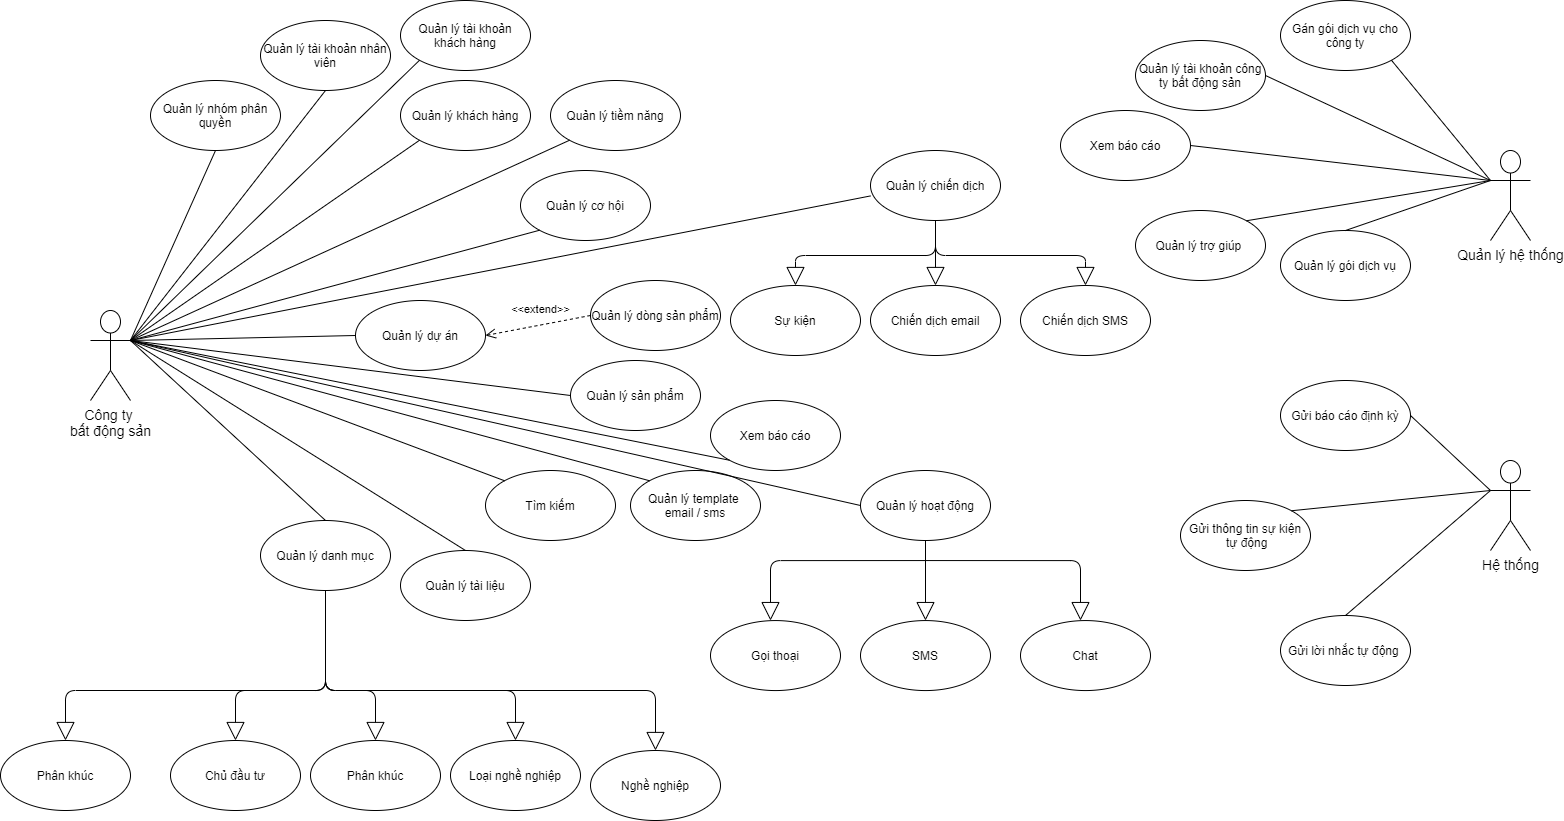
\includegraphics[width=\textwidth]{Img/Usecase/usecase_all.png}
        \vspace{0.5cm}
        \caption{Usecase tổng quát toàn hệ thống}
        \label{usecaseall}
    \end{figure}

    \begin{figure}[H]
        \centering 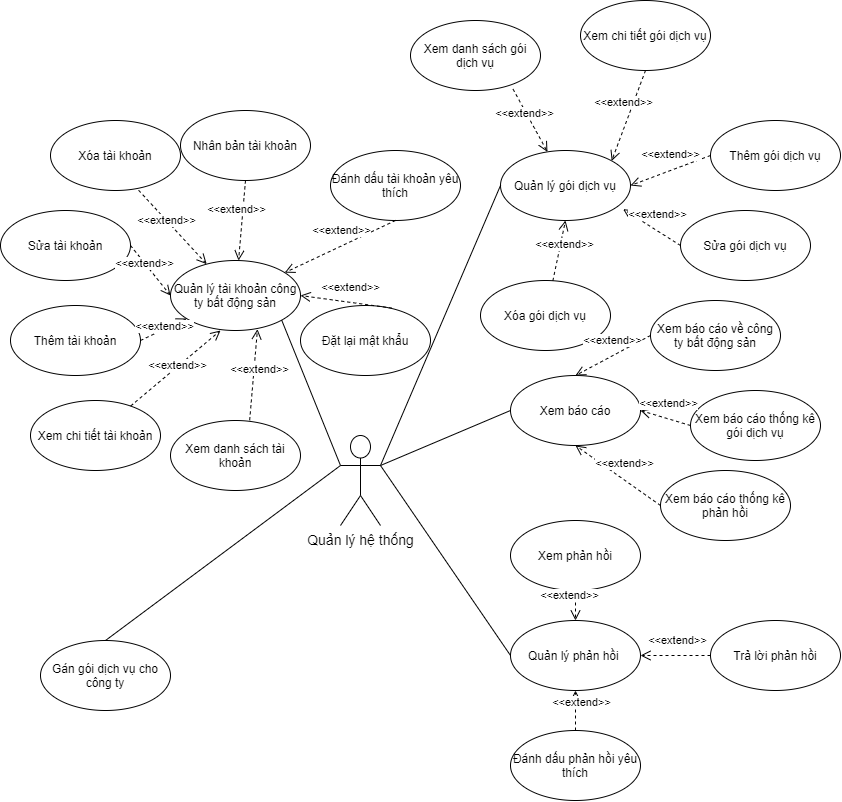
\includegraphics[width=\textwidth]{Img/Usecase/usecase_admin.png}
        \vspace{0.5cm}
        \caption{Usecase cho admin - quản trị hệ thống}
        \label{usecaseadmin}
    \end{figure}


    \begin{figure}[H]
        \centering \includegraphics[width=\textwidth]{Img/Usecase/usecase_company.png}
        \vspace{0.5cm}
        \caption{Usecase cho công ty bất động sản}
        \label{usecasecompany}
    \end{figure}

    \begin{figure}[H]
        \centering 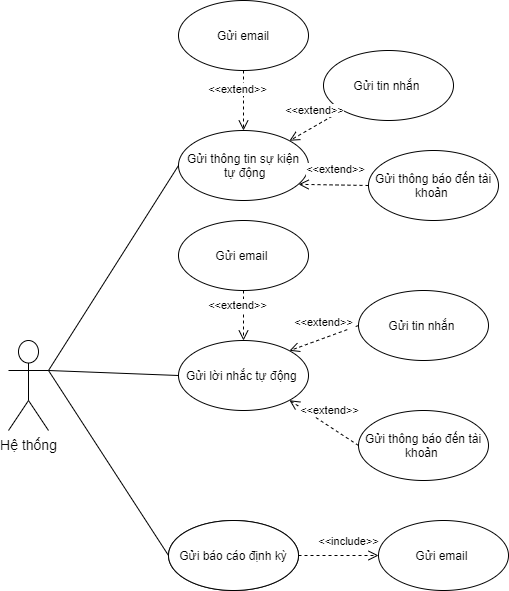
\includegraphics[width=\textwidth]{Img/Usecase/usecase_system.png}
        \vspace{0.5cm}
        \caption{Usecase cho hệ thống}
        \label{usecasesystem}
    \end{figure}



    \begin{figure}[H]
        \centering 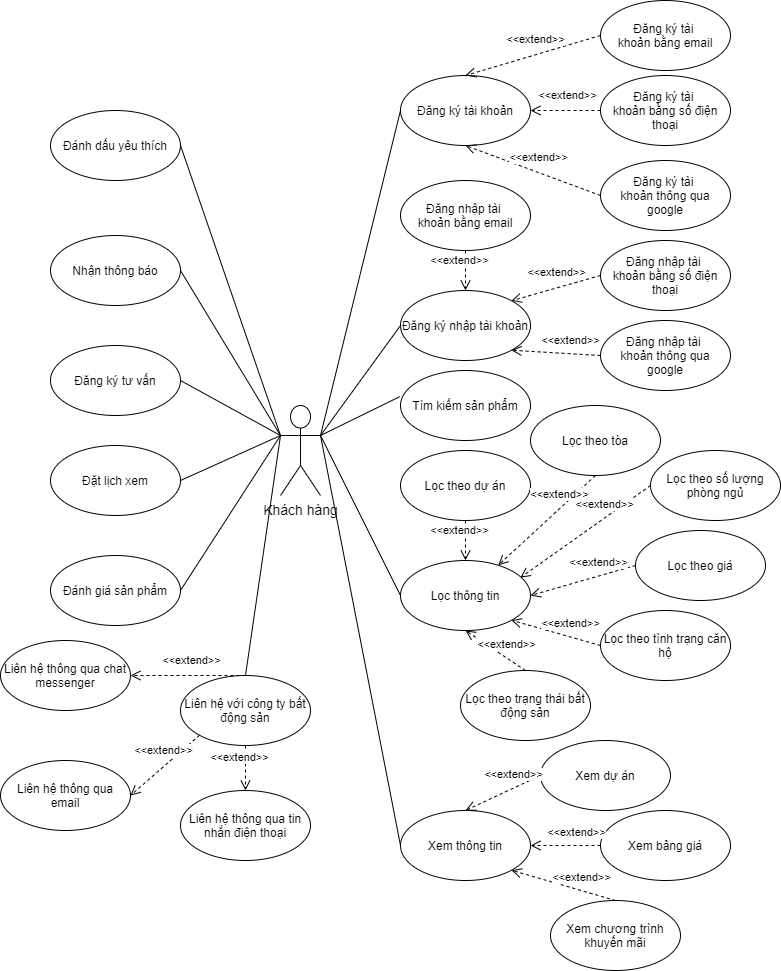
\includegraphics[width=\textwidth]{Img/Usecase/usecase_khach-hang.png}
        \vspace{0.5cm}
        \caption{Usecase cho khách hàng}
        \label{usecasecustomer}
    \end{figure}


%- Usecase diagram và mô tả usecase

    \subsubsection{Đặc tả Usecase}

% Danh sách usecase

    \begin{center}
        \begin{longtable}{|p{2.5cm}|p{4.5cm}|p{7.5cm}|c|}
            \hline
            \centering \textbf{Mã usecase} & \centering \textbf{Tên usecase} & \textbf{Mô tả}
            \\ \hline
            \endhead
            UC-001
            & Quản lý nhóm phân quyền
            & Người dùng muốn quản lý nhóm phân quyền.
            \\ \hline
            UC-001-1
            & Xem danh sách nhóm phân quyền
            & Người dùng muốn xem danh sách nhóm phân quyền.
            \\ \hline
            UC-001-2
            & Xem chi tiết nhóm phân quyền
            & Người dùng muốn xem chi tiết nhóm phân quyền.
            \\ \hline
            UC-001-3
            & Thêm nhóm phân quyền
            & Người dùng muốn thêm nhóm phân quyền.
            \\ \hline
            UC-001-4
            & Sửa nhóm phân quyền
            & Người dùng muốn sửa nhóm phân quyền.
            \\ \hline
            UC-001-5
            & Xóa nhóm phân quyền
            & Người dùng muốn xóa nhóm phân quyền.
            \\ \hline
            UC-001-6
            & Nhân bản nhóm phân quyền
            & Người dùng muốn nhân bản nhóm phân quyền.
            \\ \hline
            UC-001-7
            & Xem lịch sử thay đổi nhóm phân quyền
            & Người dùng muốn xem lịch sử nhóm phân quyền.
            \\ \hline
            UC-001-8
            & Thêm tài khoản vào nhóm phân quyền
            & Người dùng muốn thêm tài khoản nhóm phân quyền.
            \\ \hline
            UC-002
            & Quản lý tài khoản
            & Người dùng muốn quản lý tài khoản.
            %Quản lý tài khoản khách hàng
            \\ \hline

            UC-002-1
            & Quản lý tài khoản khách hàng
            & Người dùng muốn quản lý tài khoản khách hàng.
            \\ \hline
            UC-002-2
            & Quản lý tài khoản nhân viên
            & Người dùng muốn quản lý tài khoản nhân viên.
            \\ \hline
            UC-002-3
            & Xem danh sách tài khoản
            & Người dùng muốn xem danh sách tài khoản.
            \\ \hline
            UC-002-4
            & Xem chi tiết tài khoản
            & Người dùng muốn xem chi tiết tài khoản.
            \\ \hline
            UC-002-5
            & Tạo tài khoản
            & Người dùng muốn tạo tài khoản.
            \\ \hline
            UC-002-6
            & Sửa tài khoản
            & Người dùng muốn sửa tài khoản.
            \\ \hline
            UC-002-7
            & Xóa tài khoản
            & Người dùng muốn xóa tài khoản.
            \\ \hline
            UC-002-8
            & Nhân bản tài khoản
            & Người dùng muốn nhân bản tài khoản.
            \\ \hline
            UC-002-9
            & Đặt lại mật khẩu tài khoản
            & Người dùng muốn đặt lại mật khẩu tài khoản.
            \\ \hline
            UC-002-10
            & Đánh dấu yêu thích tài khoản
            & Người dùng muốn đánh dấu yêu thích tài khoản.
            \\ \hline
            UC-002-11
            & Xem lịch sử thay đổi tài khoản
            & Người dùng muốn xem lịch sử thay đổi tài khoản.
            \\ \hline
            UC-002-12
            & Nhập danh sách tài khoản khách hàng
            & Người dùng muốn nhập danh sách tài khoản khách hàng từ file.
            \\ \hline
            UC-002-13
            & Xuất danh sách tài khoản khách hàng
            & Người dùng muốn xuất danh sách tài khoản khách hàng thành file.
            \\ \hline
            UC-002-14
            & Thêm vào nhóm phân quyền
            & Người dùng muốn thêm tài khoản nhân viên vào nhóm phân quyền.
            \\ \hline
            UC-002-15
            & Thêm quyền hạn rời rạc
            & Người dùng muốn thêm quyền hạn rời rạc cho tài khoản nhân viên.
            %Xem báo cáo
            \\ \hline
            UC-003
            & Xem báo cáo
            & Người dùng muốn xem báo cáo.
            \\ \hline
            UC-003-1
            & Xem báo cáo về khách hàng
            & Người dùng muốn xem báo cáo về khách hàng.
            \\ \hline
            UC-003-2
            & Xem báo cáo về tiềm năng
            & Người dùng muốn xem báo cáo về tiềm năng.
            \\ \hline
            UC-003-3
            & Xem báo cáo về cơ hội
            & Người dùng muốn xem báo cáo về cơ hội.
            \\ \hline
            UC-003-4
            & Xem báo cáo về dự án
            & Người dùng muốn xem báo cáo về dự án.
            %Quản lý tiềm năng
            \\ \hline
            UC-004
            & Quản lý tiềm năng
            & Người dùng muốn quản lý tiềm năng.
            \\ \hline
            UC-004-1
            & Xem danh sách tiềm năng
            & Người dùng muốn xem danh sách tiềm năng.
            \\ \hline
            UC-004-2
            & Xem chi tiết tiềm năng
            & Người dùng muốn xem chi tiết tiềm năng.
            \\ \hline
            UC-004-3
            & Tạo tiềm năng
            & Người dùng muốn tạo tiềm năng.
            \\ \hline
            UC-004-4
            & Sửa tiềm năng
            & Người dùng muốn sửa tiềm năng.
            \\ \hline
            UC-004-5
            & Xóa tiềm năng
            & Người dùng muốn xóa tiềm năng.
            \\ \hline
            UC-004-6
            & Nhân bản tiềm năng
            & Người dùng muốn nhân bản tiềm năng.
            \\ \hline
            UC-004-7
            & Đánh dấu tiềm năng yêu thích
            & Người dùng muốn dánh dấu tiềm năng yêu thích.
            \\ \hline
            UC-004-8
            & Xem lịch sử thay đổi tiềm năng
            & Người dùng muốn xem lịch sử thay đổi tiềm năng.
            \\ \hline
            UC-004-9
            & Nhập danh sách tiềm năng
            & Người dùng muốn nhập danh sách cho tiềm năng.
            \\ \hline
            UC-004-10
            & Xuất danh sách tiềm năng
            & Người dùng muốn xuất danh sách cho tiềm năng.
            \\ \hline
            UC-004-11
            & Chuyển đổi tiềm năng thành khách hàng
            & Người dùng muốn chuyển đổi tiềm năng thành khách hàng.
            \\ \hline
            UC-004-12
            & Tạo cơ hội cho tiềm năng
            & Người dùng muốn tạo cơ hội cho tiềm năng.
            %Quản lý khách hàng
            \\ \hline
            UC-005
            & Quản lý khách hàng
            & Người dùng muốn quản lý khách hàng.
            \\ \hline
            UC-005-1
            & Xem danh sách khách hàng
            & Người dùng muốn xem danh sách khách hàng.
            \\ \hline
            UC-005-2
            & Xem chi tiết khách hàng
            & Người dùng muốn xem chi tiết khách hàng.
            \\ \hline
            UC-005-3
            & Tạo khách hàng
            & Người dùng muốn tạo khách hàng.
            \\ \hline
            UC-005-4
            & Sửa khách hàng
            & Người dùng muốn sửa khách hàng.
            \\ \hline
            UC-005-5
            & Xóa khách hàng
            & Người dùng muốn xóa khách hàng.
            \\ \hline
            UC-005-6
            & Nhân bản khách hàng
            & Người dùng muốn nhân bản khách hàng.
            \\ \hline
            UC-005-7
            & Đánh dấu khách hàng yêu thích
            & Người dùng muốn dánh dấu khách hàng yêu thích.
            \\ \hline
            UC-005-8
            & Xem lịch sử thay đổi khách hàng
            & Người dùng muốn xem lịch sử thay đổi khách hàng.
            \\ \hline
            UC-005-9
            & Nhập danh sách khách hàng
            & Người dùng muốn nhập danh sách cho khách hàng.
            \\ \hline
            UC-005-10
            & Xuất danh sách khách hàng
            & Người dùng muốn xuất danh sách cho khách hàng.
            \\ \hline
            UC-005-11
            & Tạo tài khoản cho khách hàng
            & Người dùng muốn tạo tài khoản cho khách hàng.
            \\ \hline
            UC-005-12
            & Tạo cơ hội cho khách hàng
            & Người dùng muốn tạo cơ hội cho khách hàng.
            %Đề xuất
            \\ \hline
            UC-006
            & Quản lý đề xuất
            & Người dùng muốn quản lý đề xuất.
            \\ \hline
            UC-006-1
            & Xem danh sách đề xuất cho khách hàng
            & Người dùng muốn xem danh sách đề xuất cho khách hàng.
            \\ \hline
            UC-006-2
            & Xem danh sách đề xuất cho tiềm năng
            & Người dùng muốn xem danh sách đề xuất cho tiềm năng.
            \\ \hline
            UC-006-3
            & Xem danh sách đề xuất cho dòng sản phẩm
            & Người dùng muốn xem danh sách đề xuất cho dòng sản phẩm.
            \\ \hline
            UC-006-4
            & Tạo cơ hội cho đề xuất
            & Người dùng muốn tạo cơ hội cho đề xuất.
            %Quản lý cơ hội
            \\ \hline
            UC-007
            & Quản lý cơ hội
            & Người dùng muốn quản lý cơ hội.
            \\ \hline
            UC-007-1
            & Xem danh sách cơ hội
            & Người dùng muốn xem danh sách cơ hội.
            \\ \hline
            UC-007-2
            & Xem chi tiết cơ hội
            & Người dùng muốn xem chi tiết cơ hội.
            \\ \hline
            UC-007-3
            & Tạo cơ hội mới
            & Người dùng muốn tạo cơ hội.
            \\ \hline
            UC-007-4
            & Tạo cơ hội từ tiềm năng
            & Người dùng muốn tạo cơ hội từ tiềm năng.
            \\ \hline
            UC-007-5
            & Tạo cơ hội từ khách hàng
            & Người dùng muốn tạo cơ hội từ khách hàng.
            \\ \hline
            UC-007-6
            & Sửa cơ hội
            & Người dùng muốn sửa cơ hội.
            \\ \hline
            UC-007-7
            & Xóa cơ hội
            & Người dùng muốn xóa cơ hội.
            \\ \hline
            UC-007-8
            & Nhân bản cơ hội
            & Người dùng muốn nhân bản cơ hội.
            \\ \hline
            UC-007-9
            & Đánh dấu cơ hội yêu thích
            & Người dùng muốn dánh dấu cơ hội yêu thích.
            \\ \hline
            UC-007-10
            & Xem lịch sử thay đổi cơ hội
            & Người dùng muốn xem lịch sử thay đổi cơ hội.
            \\ \hline
            UC-007-11
            & Xuất danh sách cơ hội
            & Người dùng muốn xuất danh sách cho cơ hội.
            %Quản lý chiến dịch
            \\ \hline
            UC-008
            & Quản lý chiến dịch
            & Người dùng muốn quản lý chiến dịch.
            \\ \hline
            UC-008-1
            & Xem danh sách chiến dịch
            & Người dùng muốn xem danh sách chiến dịch.
            \\ \hline
            UC-008-2
            & Xem chi tiết chiến dịch
            & Người dùng muốn xem chi tiết chiến dịch.
            \\ \hline
            UC-008-3
            & Tạo chiến dịch
            & Người dùng muốn tạo chiến dịch.
            \\ \hline
            UC-008-4
            & Sửa chiến dịch
            & Người dùng muốn sửa chiến dịch.
            \\ \hline
            UC-008-5
            & Xóa chiến dịch
            & Người dùng muốn xóa chiến dịch.
            \\ \hline
            UC-008-6
            & Nhân bản chiến dịch
            & Người dùng muốn nhân bản chiến dịch.
            \\ \hline
            UC-008-7
            & Đánh dấu chiến dịch yêu thích
            & Người dùng muốn dánh dấu chiến dịch yêu thích.
            \\ \hline
            UC-008-8
            & Xem lịch sử thay đổi chiến dịch
            & Người dùng muốn xem lịch sử thay đổi chiến dịch.
            \\ \hline
            UC-008-9
            & Xuất danh sách chiến dịch
            & Người dùng muốn xuất danh sách cho chiến dịch.
            %Quản lý dự án
            \\ \hline
            UC-009
            & Quản lý dự án
            & Người dùng muốn quản lý dự án.
            \\ \hline
            UC-009-1
            & Xem danh sách dự án
            & Người dùng muốn xem danh sách dự án.
            \\ \hline
            UC-009-2
            & Xem chi tiết dự án
            & Người dùng muốn xem chi tiết dự án.
            \\ \hline
            UC-009-3
            & Tạo dự án
            & Người dùng muốn tạo dự án.
            \\ \hline
            UC-009-4
            & Sửa dự án
            & Người dùng muốn sửa dự án.
            \\ \hline
            UC-009-5
            & Xóa dự án
            & Người dùng muốn xóa dự án.
            \\ \hline
            UC-009-6
            & Nhân bản dự án
            & Người dùng muốn nhân bản dự án.
            \\ \hline
            UC-009-7
            & Đánh dấu dự án yêu thích
            & Người dùng muốn dánh dấu dự án yêu thích.
            \\ \hline
            UC-009-8
            & Xem lịch sử thay đổi dự án
            & Người dùng muốn xem lịch sử thay đổi dự án.
            \\ \hline
            UC-009-9
            & Nhập danh sách dự án
            & Người dùng muốn nhập danh sách cho dự án.
            \\ \hline
            UC-009-10
            & Xuất danh sách dự án
            & Người dùng muốn xuất danh sách cho dự án.
            \\ \hline
            UC-009-11
            & Quản lý dòng sản phẩm
            & Người dùng muốn quản lý dòng sản phẩm.
            %Quản lý sản phẩm
            \\ \hline
            UC-010
            & Quản lý sản phẩm
            & Người dùng muốn quản lý sản phẩm.
            \\ \hline
            UC-010-1
            & Xem danh sách sản phẩm
            & Người dùng muốn xem danh sách sản phẩm.
            \\ \hline
            UC-010-2
            & Xem chi tiết sản phẩm
            & Người dùng muốn xem chi tiết sản phẩm.
            \\ \hline
            UC-010-3
            & Tạo sản phẩm
            & Người dùng muốn tạo sản phẩm.
            \\ \hline
            UC-010-4
            & Sửa sản phẩm
            & Người dùng muốn sửa sản phẩm.
            \\ \hline
            UC-010-5
            & Xóa sản phẩm
            & Người dùng muốn xóa sản phẩm.
            \\ \hline
            UC-010-6
            & Nhân bản sản phẩm
            & Người dùng muốn nhân bản sản phẩm.
            \\ \hline
            UC-010-7
            & Xem lịch sử thay đổi sản phẩm
            & Người dùng muốn xem lịch sử thay đổi sản phẩm.
            \\ \hline
            UC-010-8
            & Nhập danh sách sản phẩm
            & Người dùng muốn nhập danh sách cho sản phẩm.
            \\ \hline
            UC-010-9
            & Xuất danh sách sản phẩm
            & Người dùng muốn xuất danh sách cho sản phẩm.
            %Quản lý hợp đòng
            \\ \hline
            UC-011
            & Quản lý hợp đồng
            & Người dùng muốn quản lý hợp đồng.
            \\ \hline
            UC-011-1
            & Xem danh sách hợp đồng
            & Người dùng muốn xem danh sách hợp đồng.
            \\ \hline
            UC-011-2
            & Xem chi tiết hợp đồng
            & Người dùng muốn xem chi tiết hợp đồng.
            \\ \hline
            UC-011-3
            & Tạo hợp đồng
            & Người dùng muốn tạo hợp đồng.
            \\ \hline
            UC-011-4
            & Sửa hợp đồng
            & Người dùng muốn sửa hợp đồng.
            \\ \hline
            UC-011-5
            & Xóa hợp đồng
            & Người dùng muốn xóa hợp đồng.
            \\ \hline
            UC-011-6
            & Nhân bản hợp đồng
            & Người dùng muốn nhân bản hợp đồng.
            \\ \hline
            UC-011-7
            & Xem lịch sử thay đổi hợp đồng
            & Người dùng muốn xem lịch sử thay đổi hợp đồng.
            \\ \hline
            UC-011-8
            & Nhập danh sách hợp đồng
            & Người dùng muốn nhập danh sách hợp đồng.
            \\ \hline
            UC-011-9
            & Xuất danh sách hợp đồng
            & Người dùng muốn xuất danh sách hợp đồng.
            \\ \hline
            UC-011-10
            & Quản lý tiến độ thanh toán
            & Người dùng muốn quản lý tiến độ thanh toán của hợp đồng.
            %Quản lý hoạt động
            \\ \hline
            UC-012
            & Quản lý hoạt động
            & Người dùng muốn quản lý hoạt động.
            \\ \hline
            UC-012-1
            & Xem danh sách hoạt động
            & Người dùng muốn xem danh sách hoạt động.
            \\ \hline
            UC-012-2
            & Xem chi tiết hoạt động
            & Người dùng muốn xem chi tiết hoạt động.
            \\ \hline
            UC-012-3
            & Tạo hoạt động
            & Người dùng muốn tạo hoạt động.
            \\ \hline
            UC-012-4
            & Sửa hoạt động
            & Người dùng muốn sửa hoạt động.
            \\ \hline
            UC-012-5
            & Xóa hoạt động
            & Người dùng muốn xóa hoạt động.
            \\ \hline
            UC-012-6
            & Quản lý hoạt động gọi thoại
            & Người dùng muốn quản lý hoạt động gọi thoại.
            \\ \hline
            UC-012-7
            & Quản lý hoạt động SMS
            & Người dùng muốn quản lý hoạt động SMS.
            \\ \hline
            UC-012-8
            & Quản lý hoạt động email
            & Người dùng muốn quản lý hoạt động email.
            %Quản lý tài liệu
            \\ \hline
            UC-013
            & Quản lý tài liệu
            & Người dùng muốn quản lý tài liệu.
            \\ \hline
            UC-013-1
            & Xem danh sách tài liệu
            & Người dùng muốn xem danh sách tài liệu.
            \\ \hline
            UC-013-2
            & Xem chi tiết tài liệu
            & Người dùng muốn xem chi tiết tài liệu.
            \\ \hline
            UC-013-3
            & Thêm tài liệu
            & Người dùng muốn thêm tài liệu.
            \\ \hline
            UC-013-4
            & Xóa tài liệu
            & Người dùng muốn xóa tài liệu.
            \\ \hline
            UC-013-5
            & Tải tài liệu
            & Người dùng muốn tải tài liệu.
            %Quản lý template email/SMS
            \\ \hline
            UC-014
            & Quản lý template email/ sms
            & Người dùng muốn quản lý template email/ sms.
            \\ \hline
            UC-014-1
            & Xem danh sách template
            & Người dùng muốn xem danh sách template.
            \\ \hline
            UC-014-2
            & Xem chi tiết template
            & Người dùng muốn xem chi tiết template.
            \\ \hline
            UC-014-3
            & Thêm template
            & Người dùng muốn thêm template.
            \\ \hline
            UC-014-4
            & Sửa template
            & Người dùng muốn sửa template.
            \\ \hline
            UC-014-5
            & Xóa template
            & Người dùng muốn xóa template.
            %Xem Tìm kiếm
            \\ \hline
            UC-015
            & Tìm kiếm
            & Người dùng muốn tìm kiếm.
            %Usecase Admin
            %Xem quản lý tài khoản công ty bất động sản
            \\ \hline
            UC-016
            & Quản lý tài khoản công ty bất động sản
            & Người dùng muốn quản lý tài khoản công ty bất động sản.
            \\ \hline
            UC-016-1
            & Xem danh sách tài khoản công ty bất động sản
            & Người dùng muốn xem danh sách tài khoản công ty bất động sản.
            \\ \hline
            UC-016-2
            & Xem chi tiết tài khoản công ty bất động sản
            & Người dùng muốn xem chi tiết tài khoản công ty bất động sản.
            \\ \hline
            UC-016-3
            & Thêm tài khoản công ty bất động sản
            & Người dùng muốn thêm tài khoản công ty bất động sản.
            \\ \hline
            UC-016-4
            & Sửa tài khoản công ty bất động sản
            & Người dùng muốn sửa tài khoản công ty bất động sản.
            \\ \hline
            UC-016-5
            & Xóa tài khoản công ty bất động sản
            & Người dùng muốn xóa tài khoản công ty bất động sản.
            \\ \hline
            UC-016-6
            & Nhân bản tài khoản công ty bất động sản
            & Người dùng muốn nhân bản tài khoản công ty bất động sản.
            \\ \hline
            UC-016-7
            & Đánh dấu yêu thích tài khoản công ty bất động sản
            & Người dùng muốn đánh dấu yêu thích tài khoản công ty bất động sản.
            \\ \hline
            UC-016-8
            & Đặt lại mật khẩu tài khoản công ty bất động sản
            & Người dùng muốn đặt lại mật khẩu tài khoản công ty bất động sản.
            %Quản lý gói dịch vụ
            \\ \hline
            UC-017
            & Quản lý gói dịch vụ
            & Người dùng muốn quản lý gói dịch vụ công ty bất động sản.
            \\ \hline
            UC-017-1
            & Xem danh sách gói dịch vụ
            & Người dùng muốn xem danh sách gói dịch vụ công ty bất động sản.
            \\ \hline
            UC-017-2
            & Xem chi tiết gói dịch vụ
            & Người dùng muốn xem chi tiết gói dịch vụ công ty bất động sản.
            \\ \hline
            UC-017-3
            & Thêm gói dịch vụ
            & Người dùng muốn thêm gói dịch vụ công ty bất động sản.
            \\ \hline
            UC-017-4
            & Sửa danh sách gói dịch vụ
            & Người dùng muốn xem sửa gói dịch vụ công ty bất động sản.
            \\ \hline
            UC-017-5
            & Xóa danh sách gói dịch vụ
            & Người dùng muốn xóa gói dịch vụ công ty bất động sản.
            %Xem báo cáo
            \\ \hline
            UC-018
            & Xem báo cáo
            & Người dùng muốn xem báo cáo liên quan.
            \\ \hline
            UC-018-1
            & Xem báo cáo về công ty bất động sản
            & Người dùng muốn xem báo cáo về công ty bất động sản.
            \\ \hline
            UC-018-2
            & Xem báo cáo thống kê gói dịch vụ
            & Người dùng muốn xem báo cáo thống kế gói dịch vụ.
            \\ \hline
            UC-018-3
            & Xem báo cáo thống kê phản hồi
            & Người dùng muốn xem báo cáo thống kê phản hồi.
            %Quản lý phản hồi
            \\ \hline
            UC-019
            & Quản lý phản hồi
            & Người dùng muốn quản lý phản hồi.
            \\ \hline
            UC-019-1
            & Xem phản hồi
            & Người dùng muốn xem phản hồi từ người dùng hệ thống.
            \\ \hline
            UC-019-2
            & Trả lời phản hồi
            & Người dùng muốn trả lời phản hồi.
            \\ \hline
            UC-019-3
            & Đánh dấu yêu thích phản hồi
            & Người dùng muốn đánh dấu yêu thích phản hồi.
            %Gán gói dịch vụ cho công ty
            \\ \hline
            UC-020
            & Gán gói dịch vụ cho công ty
            & Người dùng muốn gán gói dịch vụ cho công ty bất động sản.
            %Hệ thống
            \\ \hline
            UC-021
            & Gửi thông tin sự kiện tự động
            & Hệ thống gửi thông tin sự kiện tự động.
            \\ \hline
            UC-021-1
            & Gửi email
            & Hệ thống gửi thông tin sự kiện tự động quan email.
            \\ \hline
            UC-021-2
            & Gửi tin nhắn
            & Hệ thống gửi thông tin sự kiện tự động qua tin nhắn.
            \\ \hline
            UC-021-3
            & Gửi thông báo đến tài khoản
            & Hệ thống gửi thông tin sự kiện tự động đến tài khoản.
            %Lời nhắc tự động
            \\ \hline
            UC-022
            & Gửi lời nhắc tự động
            & Hệ thống gửi lời nhắc tự động.
            \\ \hline
            UC-022-1
            & Gửi email
            & Hệ thống gửi lời nhắc tự động qua email.
            \\ \hline
            UC-022-2
            & Gửi tin nhắn
            & Hệ thống gửi lời nhắc tự động qua tin nhắn.
            \\ \hline
            UC-022-3
            & Gửi thông báo đến tài khoản
            & Hệ thống gửi thông báo tự động đến tài khoản người dùng.
            %Gửi báo cáo tự động
            \\ \hline
            UC-023
            & Gửi báo cáo định kỳ
            & Hệ thống gửi báo cáo định kỳ cho người dùng.
            \\ \hline
            UC-023-1
            & Gửi email
            & Hệ thống gửi báo cáo định kỳ qua email cho người dùng.
            %Khách hàng
            \\ \hline
            UC-024
            & Đăng ký tài khoản
            & Người dùng muốn đăng ký tài khoản trên hệ thống dành cho khách hàng.
            \\ \hline
            UC-024-1
            & Đăng ký tài khoản bằng email
            & Người dùng muốn đăng ký tài khoản bằng email trên hệ thống dành cho khách hàng.
            \\ \hline
            UC-024-2
            & Đăng ký tài khoản bằng số điện thoại
            & Người dùng muốn đăng ký tài khoản bằng số điện thoại trên hệ thống dành cho khách hàng.
            \\ \hline
            UC-024-3
            & Đăng ký tài khoản thông qua google
            & Người dùng muốn đăng ký tài khoản thông qua google trên hệ thống dành cho khách hàng.
            \\ \hline
            UC-025
            & Tìm kiếm sản phẩm
            & Người dùng muốn tìm kiếm sản phẩm trên hệ thống dành cho khách hàng.
            \\ \hline
            UC-026
            & Lọc thông tin
            & Người dùng muốn lọc thông tin trên hệ thống dành cho khách hàng.
            \\ \hline
            UC-026-1
            & Lọc thông tin theo dự án
            & Người dùng muốn lọc thông tin theo dự án trên hệ thống dành cho khách hàng.
            \\ \hline
            UC-026-2
            & Lọc thông tin theo tòa
            & Người dùng muốn lọc thông tin theo tòa trên hệ thống dành cho khách hàng.
            \\ \hline
            UC-026-3
            & Lọc thông tin theo số lượng phòng ngủ
            & Người dùng muốn lọc thông tin theo số lượng phòng ngủ trên hệ thống dành cho khách hàng.
            \\ \hline
            UC-026-4
            & Lọc thông tin theo giá
            & Người dùng muốn lọc thông tin theo giá trên hệ thống dành cho khách hàng.
            \\ \hline
            UC-026-5
            & Lọc thông tin theo tình trạng căn hộ
            & Người dùng muốn lọc thông tin theo tình trạng căn hộ trên hệ thống dành cho khách hàng.
            \\ \hline
            UC-026-6
            & Lọc thông tin theo tình trạng bất động sản
            & Người dùng muốn lọc thông tin theo tình trạng bất động sản trên hệ thống dành cho khách hàng.
            %Xem thông tin
            \\ \hline
            UC-027
            & Xem thông tin
            & Người dùng muốn xem thông tin trên hệ thống dành cho khách hàng.
            \\ \hline
            UC-027-1
            & Xem dự án
            & Người dùng muốn xem dự án trên hệ thống dành cho khách hàng.
            \\ \hline
            UC-027-2
            & Xem bảng giá
            & Người dùng muốn xem bảng giá trên hệ thống dành cho khách hàng.
            \\ \hline
            UC-027-3
            & Xem chương trình khuyến mãi
            & Người dùng muốn xem chương trình khuyến mãi trên hệ thống dành cho khách hàng.
            %Liên hệ với công ty bất động sản
            \\ \hline
            UC-028
            & Liên hệ với công ty bất động sản
            & Người dùng muốn liên hệ với công ty bất động sản hệ thống dành cho khách hàng.
            \\ \hline
            UC-028-1
            & Liên hệ thông qua chat messenger
            & Người dùng muốn liên hệ với công ty bất động sản thông qua chat messenger trên hệ thống dành cho khách hàng.
            \\ \hline
            UC-028-2
            & Liên hệ thông qua email
            & Người dùng muốn liên hệ với công ty bất động sản thông qua email trên hệ thống dành cho khách hàng.
            \\ \hline
            UC-028-3
            & Liên hệ thông qua tin nhắn điện thoại
            & Người dùng muốn liên hệ với công ty bất động sản thông qua tin nhắn điện thoại trên hệ thống dành cho khách hàng.
            %Đánh giá sản phẩm
            \\ \hline
            UC-029
            & Đánh giá sản phẩm
            & Người dùng muốn đánh giá sản phẩm trên hệ thống dành cho khách hàng.
            \\ \hline
            UC-030
            & Đặt lịch xem
            & Người dùng muốn đặt lịch xem bất động sản trên hệ thống dành cho khách hàng.
            \\ \hline
            UC-031
            & Đăng ký tư vấn
            & Người dùng muốn đăng ký tư vấn bất động sản trên hệ thống dành cho khách hàng.
            \\ \hline
            UC-032
            & Nhận thông báo
            & Người dùng muốn nhận thống báo hệ thống dành cho khách hàng.
            \\ \hline
            UC-033
            & Đánh dấu yêu thích
            & Người dùng muốn đánh dấu yêu thích trên hệ thống dành cho khách hàng.
            \\ \hline
            \caption{Bảng danh sách các usecase}
            \label{Bangusecases}
        \end{longtable}

    \end{center}
%Usecase xem chi tiết
    \subsubsection*{Use case xem chi tiết nhóm phân quyền }
    \begin{table}[H]
        \centering
        \begin{tabular}{|p{3.5cm}|p{11.5cm}|c|}
            \hline
            Mã Usecase      & UC-001-2                                                             \\
            \hline
            Tên usecase     & Xem chi tiết nhóm phân quyền                                         \\
            \hline
            Các tác nhân    & Quản lý của công ty bất động sản                                     \\
            \hline
            Mô tả chung     & Người dùng muốn xem chi tiết nhóm phân quyền.                        \\
            \hline
            Điều kiện trước & Người dùng đăng nhập vào hệ thống và truy cập trang nhóm phân quyền. \\
            \hline
            Điều kiện sau   & Không có                                                             \\
            \hline
            Luồng sự kiện chính & \vspace{-.8cm}\begin{enumerate}
                                                    \item Người dùng truy cập vào trang nhóm phân quyền.
                                                    \item Hệ thống hiển thị danh sách nhóm phân quyền.
                                                    \item Người dùng bấm vào nhóm phân quyền cần xem.
                                                    \item Hệ thống hiển thị trang chi tiết nhóm phân quyền.
            \end{enumerate}
            \\
            \hline
            Luồng thay thế & Tại bước 1\newline
            \vspace{-.8cm}\begin{itemize}
                              \item Nếu người dùng chưa đăng nhập thì hệ thống sẽ chuyển sang trang đăng nhập.
                              \item  Nếu người dùng không có chức năng này thì hệ thống sẽ thông báo người dùng không được phép thực hiện tính năng này.
            \end{itemize}
            \\    \hline
        \end{tabular}
        \caption{Use case xem chi tiết nhóm phân quyền }
    \end{table}


%Usecase thêm
    \subsubsection*{Use case thêm nhóm phân quyền }
    \begin{table}[H]
        \centering
        \begin{tabular}{|p{3.5cm}|p{11.5cm}|c|}
            \hline
            Mã Usecase      & UC-001-3                                                             \\
            \hline
            Tên usecase     & Thêm nhóm phân quyền                                                 \\
            \hline
            Các tác nhân    & Quản lý của công ty bất động sản                                     \\
            \hline
            Mô tả chung     & Người dùng muốn thêm nhóm phân quyền.                                \\
            \hline
            Điều kiện trước & Người dùng đăng nhập vào hệ thống và truy cập trang nhóm phân quyền. \\
            \hline
            Điều kiện sau   & Thông báo thêm nhóm phân quyền thành công/ thất bại.                 \\
            \hline
            Luồng sự kiện chính & \vspace{-.8cm}\begin{enumerate}
                                                    \item Người dùng truy cập vào trang nhóm phân quyền
                                                    \item  Người dùng bấm nút tạo nhóm phân quyền.
                                                    \item  Hệ thống hiện thị cửa sổ với các thông tin cần thiết để tạo nhóm phân quyền.
                                                    \item  Người dùng nhập dữ liệu nhóm phân quyền mới.
                                                    \item Người dùng bấm nút lưu.
                                                    \item Hệ thống kiểm tra dữ liệu nhập, nếu hợp lệ tạo nhóm phân quyền mới, còn không thì yêu cầu nhập lại.
            \end{enumerate}
            \\
            \hline
            Luồng thay thế & Tại bước 1\newline
            \vspace{-.8cm}\begin{itemize}
                              \item Nếu người dùng chưa đăng nhập thì hệ thống sẽ chuyển sang trang đăng nhập.
                              \item  Nếu người dùng không có chức năng này thì hệ thống sẽ thông báo người dùng không được phép thực hiện tính năng này.
            \end{itemize}
            \\
            \hline
        \end{tabular}
        \caption{Use case thêm nhóm phân quyền }
    \end{table}


%Usecase sửa
    \subsubsection*{Use case sửa nhóm phân quyền }
    \begin{table}[H]
        \centering
        \begin{tabular}{|p{3.5cm}|p{11.5cm}|c|}
            \hline
            Mã Usecase      & UC-001-4                                                             \\
            \hline
            Tên usecase     & Sửa nhóm phân quyền                                                  \\
            \hline
            Các tác nhân    & Quản lý của công ty bất động sản                                     \\
            \hline
            Mô tả chung     & Người dùng muốn sửa nhóm phân quyền.                                 \\
            \hline
            Điều kiện trước & Người dùng đăng nhập vào hệ thống và truy cập trang nhóm phân quyền. \\
            \hline
            Điều kiện sau   & Thông báo sửa nhóm phân quyền thành công/ thất bại.                  \\
            \hline
            Luồng sự kiện chính & \vspace{-.8cm}\begin{enumerate}
                                                    \item Người dùng truy cập vào trang nhóm phân quyền
                                                    \item  Người dùng bấm nút sửa nhóm phân quyền.
                                                    \item  Hệ thống hiện thị cửa sổ với các thông tin cần thiết để sửa nhóm phân quyền.
                                                    \item  Người dùng nhập dữ liệu cần sửa nhóm phân quyền.
                                                    \item Người dùng bấm nút lưu.
                                                    \item Hệ thống kiểm tra dữ liệu nhập, nếu hợp lệ cập nhật thông tin mới nhóm phân quyền, còn không thì yêu cầu nhập lại.
            \end{enumerate}
            \\
            \hline
            Luồng thay thế & Tại bước 1\newline
            \vspace{-.8cm}\begin{itemize}
                              \item Nếu người dùng chưa đăng nhập thì hệ thống sẽ chuyển sang trang đăng nhập.
                              \item  Nếu người dùng không có chức năng này thì hệ thống sẽ thông báo người dùng không được phép thực hiện tính năng này.
            \end{itemize}
            \\
            \hline
        \end{tabular}
        \caption{Use case sửa nhóm phân quyền }
    \end{table}


%Usecase xóa
    \subsubsection*{Use case xóa nhóm phân quyền }
    \begin{table}[H]
        \centering
        \begin{tabular}{|p{3.5cm}|p{11.5cm}|c|}
            \hline
            Mã Usecase      & UC-001-5                                                             \\
            \hline
            Tên usecase     & Xóa nhóm phân quyền                                                  \\
            \hline
            Các tác nhân    & Quản lý của công ty bất động sản                                     \\
            \hline
            Mô tả chung     & Người dùng muốn xóa nhóm phân quyền.                                 \\
            \hline
            Điều kiện trước & Người dùng đăng nhập vào hệ thống và truy cập trang nhóm phân quyền. \\
            \hline
            Điều kiện sau   & Thông báo xóa nhóm phân quyền thành công/ thất bại.                  \\
            \hline
            Luồng sự kiện chính & \vspace{-.8cm}\begin{enumerate}
                                                    \item Người dùng truy cập vào trang nhóm phân quyền.
                                                    \item Người dùng truy cập vào chi tiết nhóm phân quyền.
                                                    \item  Người dùng bấm nút xóa nhóm phân quyền.
                                                    \item  Hệ thống hiện thị thông báo chắc chắn xóa nhóm phân quyền.
                                                    \item  Người dùng bấm nút đồng ý.
                                                    \item Hệ thống kiểm tra nhóm phân quyền được yêu cầu xóa, nếu được phép xóa thì hệ thống xóa nhóm yêu cầu đó khỏi hệ thống. Nếu không được phép, hệ thống thông báo không được phép xóa nhóm phân quyền.
            \end{enumerate}
            \\
            \hline
            Luồng thay thế & Tại bước 1\newline
            \vspace{-.8cm}\begin{itemize}
                              \item Nếu người dùng chưa đăng nhập thì hệ thống sẽ chuyển sang trang đăng nhập.
                              \item Nếu người dùng không có chức năng này thì hệ thống sẽ thông báo người dùng không được phép thực hiện tính năng này.
            \end{itemize}

            Tại bước 5\newline
            \vspace{-.8cm}\begin{itemize}
                              \item Người dùng bấm nút hủy hệ thống sẽ tắt thông báo.
            \end{itemize} \\
            \hline
        \end{tabular}
        \caption{Use case xóa nhóm phân quyền }
    \end{table}


%Usecase nhân bản
    \subsubsection*{Use case nhân bản nhóm phân quyền }
    \begin{table}[H]
        \centering
        \begin{tabular}{|p{3.5cm}|p{11.5cm}|c|}
            \hline
            Mã Usecase      & UC-001-6                                                             \\
            \hline
            Tên usecase     & Nhân bản nhóm phân quyền                                             \\
            \hline
            Các tác nhân    & Quản lý của công ty bất động sản                                     \\
            \hline
            Mô tả chung     & Người dùng muốn nhân bản nhóm phân quyền.                            \\
            \hline
            Điều kiện trước & Người dùng đăng nhập vào hệ thống và truy cập trang nhóm phân quyền. \\
            \hline
            Điều kiện sau   & Thông báo nhân bản nhóm phân quyền thành công/ thất bại.             \\
            \hline
            Luồng sự kiện chính & \vspace{-.8cm}\begin{enumerate}
                                                    \item Người dùng truy cập vào trang nhóm phân quyền.
                                                    \item Người dùng truy cập vào chi tiết nhóm phân quyền.
                                                    \item  Người dùng bấm nút nhân bản nhóm phân quyền.
                                                    \item  Hệ thống hiện thị thông báo chắc chắn nhân bản nhóm phân quyền.
                                                    \item  Người dùng bấm nút đồng ý.
                                                    \item Hệ thống nhân bản nhóm phân quyền.
            \end{enumerate}
            \\
            \hline
            Luồng thay thế & Tại bước 1\newline
            \vspace{-.8cm}\begin{itemize}
                              \item Nếu người dùng chưa đăng nhập thì hệ thống sẽ chuyển sang trang đăng nhập.
                              \item Nếu người dùng không có chức năng này thì hệ thống sẽ thông báo người dùng không được phép thực hiện tính năng này.
            \end{itemize}

            Tại bước 5\newline
            \vspace{-.8cm}\begin{itemize}
                              \item Người dùng bấm nút hủy hệ thống sẽ tắt thông báo.
            \end{itemize} \\
            \hline
        \end{tabular}
        \caption{Use case nhân bản nhóm phân quyền }
    \end{table}


%Usecase Xem lịch sử thay đổi nhóm phân quyền
    \subsubsection*{Use case xem lịch sử thay đổi nhóm phân quyền }
    \begin{table}[H]
        \centering
        \begin{tabular}{|p{3.5cm}|p{11.5cm}|c|}
            \hline
            Mã Usecase      & UC-001-7                                                             \\
            \hline
            Tên usecase     & Xem lịch sử thay đổi nhóm phân quyền                                 \\
            \hline
            Các tác nhân    & Quản lý của công ty bất động sản                                     \\
            \hline
            Mô tả chung     & Người dùng muốn xem lịch sử nhóm phân quyền.                         \\
            \hline
            Điều kiện trước & Người dùng đăng nhập vào hệ thống và truy cập trang nhóm phân quyền. \\
            \hline
            Điều kiện sau   & Không có.                                                            \\
            \hline
            Luồng sự kiện chính & \vspace{-.8cm}\begin{enumerate}
                                                    \item Người dùng truy cập vào trang nhóm phân quyền.
                                                    \item Người dùng truy cập vào lịch sử nhóm phân quyền.
                                                    \item Hệ thống hiển thị lịch sử thay đổi nhóm phân quyền.
            \end{enumerate}
            \\
            \hline
            Luồng thay thế & Tại bước 1\newline
            \vspace{-.8cm}\begin{itemize}
                              \item Nếu người dùng chưa đăng nhập thì hệ thống sẽ chuyển sang trang đăng nhập.
                              \item Nếu người dùng không có chức năng này thì hệ thống sẽ thông báo người dùng không được phép thực hiện tính năng này.
            \end{itemize}
            \\ \hline
        \end{tabular}
        \caption{Use case xem lịch sử thay đổi nhóm phân quyền }
    \end{table}

%Usecase Thêm tài khoản vào nhóm phân quyền
    \subsubsection*{Use case thêm tài khoản vào nhóm phân quyền }

    \begin{table}[H]
        \centering
        \begin{tabular}{|p{3.5cm}|p{11.5cm}|c|}
            \hline
            Mã Usecase      & UC-001-8                                                             \\
            \hline
            Tên usecase     & Thêm tài khoản vào nhóm phân quyền                                   \\
            \hline
            Các tác nhân    & Quản lý của công ty bất động sản                                     \\
            \hline
            Mô tả chung     & Người dùng muốn thêm tài khoản vào nhóm phân quyền.                  \\
            \hline
            Điều kiện trước & Người dùng đăng nhập vào hệ thống và truy cập trang nhóm phân quyền. \\
            \hline
            Điều kiện sau   & Thông báo thêm tài khoản vào nhóm phân quyền thành công/ thất bại.   \\
            \hline
            Luồng sự kiện chính & \vspace{-.8cm}\begin{enumerate}
                                                    \item Người dùng truy cập vào trang nhóm phân quyền.
                                                    \item Người dùng bấm nút thêm tài khoản vào nhóm phân quyền.
                                                    \item Hệ thống hiển thị cửa sổ để người dùng chọn tài khoản cần thêm vào.
                                                    \item Người dùng chọn tài khoản cần thêm và bấm nút đồng ý.
                                                    \item Hệ thống thêm tài khoản vào nhóm phân quyền.
            \end{enumerate}
            \\
            \hline
            Luồng thay thế & Tại bước 1\newline
            \vspace{-.8cm}\begin{itemize}
                              \item Nếu người dùng chưa đăng nhập thì hệ thống sẽ chuyển sang trang đăng nhập.
                              \item Nếu người dùng không có chức năng này thì hệ thống sẽ thông báo người dùng không được phép thực hiện tính năng này.
            \end{itemize}
            Tại bước 5\newline
            \vspace{-.8cm}\begin{itemize}
                              \item Người dùng bấm nút hủy hệ thống tắt cửa số hiển thị.
            \end{itemize}

            \\ \hline
        \end{tabular}
        \caption{Use case thêm tài khoản vào nhóm phân quyền }
    \end{table}


%Usecase Quản lý tài khoản
    \subsubsection*{Use case quản lý tài khoản}
    \begin{table}[H]
        \centering
        \begin{tabular}{|p{3.5cm}|p{11.5cm}|c|}
            \hline
            Mã Usecase      & UC-002                             \\
            \hline
            Tên usecase     & Quản lý tài khoản                  \\
            \hline
            Các tác nhân    & Quản lý của công ty bất động sản   \\
            \hline
            Mô tả chung     & Người dùng muốn quản lý tài khoản. \\
            \hline
            Extends UseCase & Xem danh sách tài khoản, xem chi tiết tài khoản, tạo tài khoản, sửa tài khoản, xóa tài khoản, nhân bản tài khoản, đặt lại mật khẩu, đánh dấu tài khoản yêu thích, xem lịch sử thay đổi tài khoản.
            \\
            \hline
            Điều kiện trước & Người dùng đăng nhập vào hệ thống. \\
            \hline

            Điều kiện sau   & Không có.                          \\
            \hline
            Luồng sự kiện chính & \vspace{-.8cm}\begin{enumerate}
                                                    \item Người dùng truy cập vào quản lý tài khoản.
                                                    \item Hệ thống hiển thị trang quản lý tài khoản.
                                                    \item Người dùng thao tác các tính năng theo nhu cầu.
            \end{enumerate}
            \\
            \hline
            Luồng thay thế & Tại bước 1\newline
            \vspace{-.8cm}\begin{itemize}
                              \item Nếu người dùng chưa đăng nhập thì hệ thống sẽ chuyển sang trang đăng nhập.
                              \item Nếu người dùng không có chức năng này thì hệ thống sẽ thông báo người dùng không được phép thực hiện tính năng này.
            \end{itemize}

            \\ \hline
        \end{tabular}
        \caption{Use case quản lý tài khoản}
    \end{table}


%Usecase Quản lý tài khoản khách hàng
    \subsubsection*{Use case quản lý tài khoản khách hàng}
    \begin{table}[H]
        \centering
        \begin{tabular}{|p{3.5cm}|p{11.5cm}|c|}
            \hline
            Mã Usecase      & UC-002-1                                      \\
            \hline
            Tên usecase     & Quản lý tài khoản khách hàng                  \\
            \hline
            Các tác nhân    & Quản lý và nhân viên công ty bất động sản     \\
            \hline
            Mô tả chung     & Người dùng muốn quản lý tài khoản khách hàng. \\
            \hline
            Điều kiện trước & Người dùng đăng nhập vào hệ thống.            \\
            \hline
            Điều kiện sau   & Không có.                                     \\
            \hline
            Luồng sự kiện chính & \vspace{-.8cm}\begin{enumerate}
                                                    \item Người dùng truy cập vào quản lý tài khoản khách hàng.
                                                    \item Hệ thống hiển thị trang quản lý tài khoản khách hàng.
                                                    \item Người dùng thao tác các tính năng theo nhu cầu.
            \end{enumerate}
            \\
            \hline
            Luồng thay thế & Tại bước 1\newline
            \vspace{-.8cm}\begin{itemize}
                              \item Nếu người dùng chưa đăng nhập thì hệ thống sẽ chuyển sang trang đăng nhập.
                              \item Nếu người dùng không có chức năng này thì hệ thống sẽ thông báo người dùng không được phép thực hiện tính năng này.
            \end{itemize}

            \\ \hline
        \end{tabular}
        \caption{Use case quản lý tài khoản khách hàng}
    \end{table}


%Usecase Quản lý tài khoản nhân viên
    \subsubsection*{Use case quản lý tài khoản nhân viên}
    \begin{table}[H]
        \centering
        \begin{tabular}{|p{3.5cm}|p{11.5cm}|c|}
            \hline
            Mã Usecase      & UC-002-2                                     \\
            \hline
            Tên usecase     & Quản lý tài khoản nhân viên                  \\
            \hline
            Các tác nhân    & Quản lý của công ty bất động sản             \\
            \hline
            Mô tả chung     & Người dùng muốn quản lý tài khoản nhân viên. \\
            \hline
            Điều kiện trước & Người dùng đăng nhập vào hệ thống.           \\
            \hline
            Điều kiện sau   & Không có.                                    \\
            \hline
            Luồng sự kiện chính & \vspace{-.8cm}\begin{enumerate}
                                                    \item Người dùng truy cập vào quản lý tài khoản nhân viên.
                                                    \item Hệ thống hiển thị trang quản lý tài khoản nhân viên.
                                                    \item Người dùng thao tác các tính năng theo nhu cầu.
            \end{enumerate}
            \\
            \hline
            Luồng thay thế & Tại bước 1\newline
            \vspace{-.8cm}\begin{itemize}
                              \item Nếu người dùng chưa đăng nhập thì hệ thống sẽ chuyển sang trang đăng nhập.
                              \item Nếu người dùng không có chức năng này thì hệ thống sẽ thông báo người dùng không được phép thực hiện tính năng này.
            \end{itemize}

            \\ \hline
        \end{tabular}
        \caption{Use case quản lý tài khoản nhân viên}
    \end{table}


%Usecase Xem danh sách tài khoản
    \subsubsection*{Use case xem danh tài khoản }
    \begin{table}[H]
        \centering
        \begin{tabular}{|p{3.5cm}|p{11.5cm}|c|}
            \hline
            Mã Usecase      & UC-002-3                                                       \\
            \hline
            Tên usecase     & Xem danh sách tài khoản                                        \\
            \hline
            Các tác nhân    & Quản lý, nhân viên của công ty bất động sản                    \\
            \hline
            Mô tả chung     & Người dùng muốn xem danh sách nhóm tài khoản.                  \\
            \hline
            Điều kiện trước & Người dùng đăng nhập vào hệ thống và truy cập trang tài khoản. \\
            \hline
            Điều kiện sau   & Không có                                                       \\
            \hline
            Luồng sự kiện chính & \vspace{-.8cm}\begin{enumerate}
                                                    \item Người dùng truy cập vào trang tài khoản.
                                                    \item Hệ thống hiển thị danh sách tài khoản.
            \end{enumerate}
            \\
            \hline
            Luồng thay thế & Tại bước 1\newline
            \vspace{-.8cm}\begin{itemize}
                              \item Nếu người dùng chưa đăng nhập thì hệ thống sẽ chuyển sang trang đăng nhập.
                              \item  Nếu người dùng không có chức năng này thì hệ thống sẽ thông báo người dùng không được phép thực hiện tính năng này.
            \end{itemize}

            \\    \hline
        \end{tabular}
        \caption{Use case xem danh tài khoản }
    \end{table}


%Usecase xem chi tiết tài khoản
    \subsubsection*{Use case xem chi tiết tài khoản }
    \begin{table}[H]
        \centering
        \begin{tabular}{|p{3.5cm}|p{11.5cm}|c|}
            \hline
            Mã Usecase      & UC-002-4                                                       \\
            \hline
            Tên usecase     & Xem chi tiết tài khoản                                         \\
            \hline
            Các tác nhân    & Quản lý, nhân viên của công ty bất động sản                    \\
            \hline
            Mô tả chung     & Người dùng muốn xem chi tiết tài khoản.                        \\
            \hline
            Điều kiện trước & Người dùng đăng nhập vào hệ thống và truy cập trang tài khoản. \\
            \hline
            Điều kiện sau   & Không có                                                       \\
            \hline
            Luồng sự kiện chính & \vspace{-.8cm}\begin{enumerate}
                                                    \item Người dùng truy cập vào trang tài khoản.
                                                    \item Hệ thống hiển thị danh sách trang tài khoản.
                                                    \item Người dùng bấm vào tài khoản cần xem.
                                                    \item Hệ thống hiển thị trang chi tiết tài khoản.
            \end{enumerate}
            \\
            \hline
            Luồng thay thế & Tại bước 1\newline
            \vspace{-.8cm}\begin{itemize}
                              \item Nếu người dùng chưa đăng nhập thì hệ thống sẽ chuyển sang trang đăng nhập.
                              \item  Nếu người dùng không có chức năng này thì hệ thống sẽ thông báo người dùng không được phép thực hiện tính năng này.
            \end{itemize}

            \\    \hline
        \end{tabular}
        \caption{Use case xem chi tiết tài khoản }
    \end{table}


%Usecase thêm tài khoản
    \subsubsection*{Use case tạo tài khoản }
    \begin{table}[H]
        \centering
        \begin{tabular}{|p{3.5cm}|p{11.5cm}|c|}
            \hline
            Mã Usecase      & UC-002-5                                                       \\
            \hline
            Tên usecase     & Tạo tài khoản                                                  \\
            \hline
            Các tác nhân    & Quản lý, nhân viên của công ty bất động sản                    \\
            \hline
            Mô tả chung     & Người dùng muốn thêm tài khoản.                                \\
            \hline
            Điều kiện trước & Người dùng đăng nhập vào hệ thống và truy cập trang tài khoản. \\
            \hline
            Điều kiện sau   & Thông báo thêm tài khoản thành công/ thất bại.                 \\
            \hline
            Luồng sự kiện chính & \vspace{-.8cm}\begin{enumerate}
                                                    \item Người dùng truy cập vào trang tài khoản
                                                    \item  Người dùng bấm nút tạo tài khoản.
                                                    \item  Hệ thống hiện thị cửa sổ với các thông tin cần thiết để tạo tài khoản.
                                                    \item  Người dùng nhập dữ liệu tài khoản.
                                                    \item Người dùng bấm nút lưu.
                                                    \item Hệ thống kiểm tra dữ liệu nhập, nếu hợp lệ tạo tài khoản mới, còn không thì yêu cầu nhập lại.
            \end{enumerate}
            \\
            \hline
            Luồng thay thế & Tại bước 1\newline
            \vspace{-.8cm}\begin{itemize}
                              \item Nếu người dùng chưa đăng nhập thì hệ thống sẽ chuyển sang trang đăng nhập.
                              \item  Nếu người dùng không có chức năng này thì hệ thống sẽ thông báo người dùng không được phép thực hiện tính năng này.
            \end{itemize}
            \\
            \hline
        \end{tabular}
        \caption{Use case tạo tài khoản }
    \end{table}


%Usecase sửa tài khoản
    \subsubsection*{Use case sửa tài khoản }
    \begin{table}[H]
        \centering
        \begin{tabular}{|p{3.5cm}|p{11.5cm}|c|}
            \hline
            Mã Usecase      & UC-002-6                                                       \\
            \hline
            Tên usecase     & Sửa tài khoản                                                  \\
            \hline
            Các tác nhân    & Quản lý, nhân viên của công ty bất động sản                    \\
            \hline
            Mô tả chung     & Người dùng muốn sửa tài khoản.                                 \\
            \hline
            Điều kiện trước & Người dùng đăng nhập vào hệ thống và truy cập trang tài khoản. \\
            \hline
            Điều kiện sau   & Thông báo sửa tài khoản thành công/ thất bại.                  \\
            \hline
            Luồng sự kiện chính & \vspace{-.8cm}\begin{enumerate}
                                                    \item Người dùng truy cập vào trang tài khoản
                                                    \item  Người dùng bấm nút sửa tài khoản.
                                                    \item  Hệ thống hiện thị cửa sổ với các thông tin cần thiết để sửa tài khoản.
                                                    \item  Người dùng nhập dữ liệu cần sửa tài khoản.
                                                    \item Người dùng bấm nút lưu.
                                                    \item Hệ thống kiểm tra dữ liệu nhập, nếu hợp lệ cập nhật thông tin mới tài khoản, còn không thì yêu cầu nhập lại.
            \end{enumerate}
            \\
            \hline
            Luồng thay thế & Tại bước 1\newline
            \vspace{-.8cm}\begin{itemize}
                              \item Nếu người dùng chưa đăng nhập thì hệ thống sẽ chuyển sang trang đăng nhập.
                              \item  Nếu người dùng không có chức năng này thì hệ thống sẽ thông báo người dùng không được phép thực hiện tính năng này.
            \end{itemize}
            \\
            \hline
        \end{tabular}
        \caption{Use case sửa tài khoản }
    \end{table}


%Usecase xóa tài khoản
    \subsubsection*{Use case xóa tài khoản }
    \begin{table}[H]
        \centering
        \begin{tabular}{|p{3.5cm}|p{11.5cm}|c|}
            \hline
            Mã Usecase      & UC-002-7                                                             \\
            \hline
            Tên usecase     & Xóa tài khoản                                                        \\
            \hline
            Các tác nhân    & Quản lý, nhân viên của công ty bất động sản                          \\
            \hline
            Mô tả chung     & Quản lý công ty bất động sản xóa tài khoản.                          \\
            \hline
            Điều kiện trước & Người dùng đăng nhập vào hệ thống và truy cập trang nhóm phân quyền. \\
            \hline
            Điều kiện sau   & Thông báo xóa tài khoản thành công/ thất bại.                        \\
            \hline
            Luồng sự kiện chính & \vspace{-.8cm}\begin{enumerate}
                                                    \item Người dùng truy cập vào tài khoản.
                                                    \item Người dùng truy cập vào chi tiết tài khoản.
                                                    \item  Người dùng bấm nút xóa tài khoản.
                                                    \item  Hệ thống hiện thị thông báo chắc chắn xóa tài khoản.
                                                    \item  Người dùng bấm nút đồng ý.
                                                    \item Hệ thống kiểm tra nhóm phân quyền được yêu cầu xóa, nếu được phép xóa thì hệ thống xóa tài khoản yêu cầu đó khỏi hệ thống. Nếu không được phép, hệ thống thông báo không được phép xóa tài khoản.
            \end{enumerate}
            \\
            \hline
            Luồng thay thế & Tại bước 1\newline
            \vspace{-.8cm}\begin{itemize}
                              \item Nếu người dùng chưa đăng nhập thì hệ thống sẽ chuyển sang trang đăng nhập.
                              \item Nếu người dùng không có chức năng này thì hệ thống sẽ thông báo người dùng không được phép thực hiện tính năng này.
            \end{itemize}
            Tại bước 5\newline
            \vspace{-.8cm}\begin{itemize}
                              \item Người dùng bấm nút hủy hệ thống sẽ tắt thông báo.
            \end{itemize} \\
            \hline
        \end{tabular}
        \caption{Use case xóa tài khoản }
    \end{table}


%Usecase đặt lại mật khẩu tài khoản
    \subsubsection*{Use case đặt lại mật khẩu tài khoản}
    \begin{table}[H]
        \centering
        \begin{tabular}{|p{3.5cm}|p{11.5cm}|c|}
            \hline
            Mã Usecase      & UC-002-9                                                       \\
            \hline
            Tên usecase     & Đặt lại mật khẩu tài khoản tài khoản                           \\
            \hline
            Các tác nhân    & Quản lý, nhân viên của công ty bất động sản                    \\
            \hline
            Mô tả chung     & Người dùng muốn đặt lại tài khoản.                             \\
            \hline
            Điều kiện trước & Người dùng đăng nhập vào hệ thống và truy cập trang tài khoản. \\
            \hline
            Điều kiện sau   & Thông báo đặt lại tài khoản thành công/ thất bại.              \\
            \hline
            Luồng sự kiện chính & \vspace{-.8cm}\begin{enumerate}
                                                    \item Người dùng truy cập vào trang tài khoản.
                                                    \item Người dùng truy cập vào chi tiết tài khoản.
                                                    \item  Người dùng bấm nút đặt lại tài khoản.
                                                    \item  Hệ thống hiện thị cửa sổ để nhập tài khoản mới.
                                                    \item  Người dùng bấm nút lưu.
                                                    \item Hệ thống cập nhật mật khẩu tài khoản mới.
            \end{enumerate}
            \\
            \hline
            Luồng thay thế & Tại bước 1\newline
            \vspace{-.8cm}\begin{itemize}
                              \item Nếu người dùng chưa đăng nhập thì hệ thống sẽ chuyển sang trang đăng nhập.
                              \item Nếu người dùng không có chức năng này thì hệ thống sẽ thông báo người dùng không được phép thực hiện tính năng này.
            \end{itemize}

            Tại bước 5\newline
            \vspace{-.8cm}\begin{itemize}
                              \item Người dùng bấm nút hủy hệ thống sẽ tắt cửa sổ.
            \end{itemize} \\
            \hline
        \end{tabular}
        \caption{Use case đặt lại mật khẩu tài khoản}
    \end{table}

%Usecase Đánh dấu yêu thích tài khoản
    \subsubsection*{Use case đánh dấu yêu thích tài khoản}
    \begin{table}[H]
        \centering
        \begin{tabular}{|p{3.5cm}|p{11.5cm}|c|}
            \hline
            Mã Usecase      & UC-002-10                                                      \\
            \hline
            Tên usecase     & Đánh dấu yêu thích tài khoản                                   \\
            \hline
            Các tác nhân    & Quản lý, nhân viên của công ty bất động sản                    \\
            \hline
            Mô tả chung     & Người dùng muốn đánh dấu yêu thích tài khoản.                  \\
            \hline
            Điều kiện trước & Người dùng đăng nhập vào hệ thống và truy cập trang tài khoản. \\
            \hline
            Điều kiện sau   & Không có.                                                      \\
            \hline
            Luồng sự kiện chính & \vspace{-.8cm}\begin{enumerate}
                                                    \item Người dùng truy cập vào trang tài khoản.
                                                    \item Người dùng truy cập vào chi tiết tài khoản.
                                                    \item Người dùng đánh dấu yêu thích tài khoản.
                                                    \item Hệ thống lưu tài khoản yêu thích.
            \end{enumerate}
            \\
            \hline
            Luồng thay thế & Tại bước 1\newline
            \vspace{-.8cm}\begin{itemize}
                              \item Nếu người dùng chưa đăng nhập thì hệ thống sẽ chuyển sang trang đăng nhập.
                              \item Nếu người dùng không có chức năng này thì hệ thống sẽ thông báo người dùng không được phép thực hiện tính năng này.
            \end{itemize}
            \\ \hline
        \end{tabular}
        \caption{Use case đánh dấu yêu thích tài khoản}
    \end{table}


%Usecase Xem lịch sử thay đổi tài khoản
    \subsubsection*{Use case xem lịch sử thay đổi tài khoản}
    \begin{table}[H]
        \centering
        \begin{tabular}{|p{3.5cm}|p{11.5cm}|c|}
            \hline
            Mã Usecase      & UC-002-11                                                      \\
            \hline
            Tên usecase     & Xem lịch sử thay đổi tài khoản                                 \\
            \hline
            Các tác nhân    & Quản lý, nhân viên của công ty bất động sản                    \\
            \hline
            Mô tả chung     & Người dùng muốn xem lịch sử tài khoản.                         \\
            \hline
            Điều kiện trước & Người dùng đăng nhập vào hệ thống và truy cập trang tài khoản. \\
            \hline
            Điều kiện sau   & Không có.                                                      \\
            \hline
            Luồng sự kiện chính & \vspace{-.8cm}\begin{enumerate}
                                                    \item Người dùng truy cập vào trang tài khoản.
                                                    \item Người dùng truy cập vào lịch sử tài khoản.
                                                    \item Hệ thống hiển thị lịch sử thay đổi tài khoản.
            \end{enumerate}
            \\
            \hline
            Luồng thay thế & Tại bước 1\newline
            \vspace{-.8cm}\begin{itemize}
                              \item Nếu người dùng chưa đăng nhập thì hệ thống sẽ chuyển sang trang đăng nhập.
                              \item Nếu người dùng không có chức năng này thì hệ thống sẽ thông báo người dùng không được phép thực hiện tính năng này.
            \end{itemize}
            \\ \hline
        \end{tabular}
        \caption{Use case xem lịch sử thay đổi tài khoản}
    \end{table}


%Usecase nhập danh sách tài khoản khách hàng
    \subsubsection*{Use case nhập danh sách tài khoản khách hàng}
    \begin{table}[H]
        \centering
        \begin{tabular}{|p{3.5cm}|p{11.5cm}|c|}
            \hline
            Mã Usecase      & UC-002-12                                                           \\
            \hline
            Tên usecase     & Nhập danh sách tài khoản khách hàng                                 \\
            \hline
            Các tác nhân    & Quản lý, nhân viên của công ty bất động sản                         \\
            \hline
            Mô tả chung     & Người dùng muốn nhập danh sách tài khoản khách hàng.                \\
            \hline
            Điều kiện trước & Người dùng đăng nhập vào hệ thống và truy cập trang tài khoản.      \\
            \hline
            Điều kiện sau   & Thông báo nhập danh sách tài khoản khách hàng thành công/ thất bại. \\
            \hline
            Luồng sự kiện chính & \vspace{-.8cm}\begin{enumerate}
                                                    \item Người dùng truy cập vào trang tài khoản.
                                                    \item Người dùng bấm nút nhập danh sách tài khoản.
                                                    \item Hệ thống hiển thị cửa sổ để chọn file.
                                                    \item Người dùng bấm nút đồng ý.
                                                    \item Hệ thống xử lý file và lưu tất cả tài khoản được tạo từ file vừa nhập.
            \end{enumerate}
            \\
            \hline
            Luồng thay thế & Tại bước 1\newline
            \vspace{-.8cm}\begin{itemize}
                              \item Nếu người dùng chưa đăng nhập thì hệ thống sẽ chuyển sang trang đăng nhập.
                              \item Nếu người dùng không có chức năng này thì hệ thống sẽ thông báo người dùng không được phép thực hiện tính năng này.
            \end{itemize}
            Tại bước 4\newline
            \vspace{-.8cm}\begin{itemize}
                              \item Người dùng bấm nút hủy hệ thống sẽ tắt cửa sổ hiển thị.
            \end{itemize}
            \\ \hline
        \end{tabular}
        \caption{Use case nhập danh sách tài khoản khách hàng}
    \end{table}


%Usecase xuất danh sách tài khoản khách hàng

    \subsubsection*{Use case xuất danh sách tài khoản khách hàng}
    \begin{table}[H]
        \centering
        \begin{tabular}{|p{3.5cm}|p{11.5cm}|c|}
            \hline
            Mã Usecase      & UC-002-13                                                           \\
            \hline
            Tên usecase     & Xuất danh sách tài khoản khách hàng                                 \\
            \hline
            Các tác nhân    & Quản lý, nhân viên của công ty bất động sản                         \\
            \hline
            Mô tả chung     & Người dùng muốn xuất danh sách tài khoản khách hàng.                \\
            \hline
            Điều kiện trước & Người dùng đăng nhập vào hệ thống và truy cập trang tài khoản.      \\
            \hline
            Điều kiện sau   & Thông báo xuất danh sách tài khoản khách hàng thành công/ thất bại. \\
            \hline
            Luồng sự kiện chính & \vspace{-.8cm}\begin{enumerate}
                                                    \item Người dùng truy cập vào trang tài khoản.
                                                    \item Người dùng bấm nút xuất danh sách tài khoản
                                                    \item Hệ thống tải file xuống máy người dùng.
            \end{enumerate}
            \\
            \hline
            Luồng thay thế & Tại bước 1\newline
            \vspace{-.8cm}\begin{itemize}
                              \item Nếu người dùng chưa đăng nhập thì hệ thống sẽ chuyển sang trang đăng nhập.
                              \item Nếu người dùng không có chức năng này thì hệ thống sẽ thông báo người dùng không được phép thực hiện tính năng này.
            \end{itemize}
            Tại bước 3\newline
            \vspace{-.8cm}\begin{itemize}
                              \item Nếu có lỗi trong quá trình tải file hệ thống hiển thị thông báo lỗi.
            \end{itemize}
            \\ \hline
        \end{tabular}
        \caption{Use case xuất danh sách tài khoản khách hàng}
    \end{table}

%Usecase thêm vào nhóm phân quyền

    \subsubsection*{Use case thêm vào nhóm phân quyền}
    \begin{table}[H]
        \centering
        \begin{tabular}{|p{3.5cm}|p{11.5cm}|c|}
            \hline
            Mã Usecase      & UC-002-14                                                          \\
            \hline
            Tên usecase     & Thêm vào nhóm phân quyền                                           \\
            \hline
            Các tác nhân    & Quản lý của công ty bất động sản                                   \\
            \hline
            Mô tả chung     & Người dùng muốn thêm tài khoản nhân viên vào nhóm phân quyền.      \\
            \hline
            Điều kiện trước & Người dùng đăng nhập vào hệ thống và truy cập trang tài khoản.     \\
            \hline
            Điều kiện sau   & Thông báo thêm tài khoản vào nhóm phân quyền thành công/ thất bại. \\
            \hline
            Luồng sự kiện chính & \vspace{-.8cm}\begin{enumerate}
                                                    \item Người dùng truy cập vào trang tài khoản.
                                                    \item Người dùng bấm nút thêm vào nhóm phân quyền
                                                    \item Hệ thống thêm tài khoản vào nhóm phân quyền.
            \end{enumerate}
            \\
            \hline
            Luồng thay thế & Tại bước 1\newline
            \vspace{-.8cm}\begin{itemize}
                              \item Nếu người dùng chưa đăng nhập thì hệ thống sẽ chuyển sang trang đăng nhập.
                              \item Nếu người dùng không có chức năng này thì hệ thống sẽ thông báo người dùng không được phép thực hiện tính năng này.
            \end{itemize}
            \\ \hline
        \end{tabular}
        \caption{Use case thêm vào nhóm phân quyền}
    \end{table}


%Usecase thêm vào nhóm phân quyền rời rạc

    \subsubsection*{Use case thêm vào nhóm phân quyền rời rạc}
    \begin{table}[H]
        \centering
        \begin{tabular}{|p{3.5cm}|p{11.5cm}|c|}
            \hline
            Mã Usecase      & UC-002-15                                                              \\
            \hline
            Tên usecase     & Thêm vào nhóm phân quyền rời rạc                                       \\
            \hline
            Các tác nhân    & Quản lý của công ty bất động sản                                       \\
            \hline
            Mô tả chung     & Người dùng muốn thêm tài khoản nhân viên vào từng nhóm phân quyền nhỏ. \\
            \hline
            Điều kiện trước & Người dùng đăng nhập vào hệ thống và truy cập trang tài khoản.         \\
            \hline
            Điều kiện sau   & Thông báo thêm tài khoản vào nhóm phân quyền thành công/ thất bại.     \\
            \hline
            Luồng sự kiện chính & \vspace{-.8cm}\begin{enumerate}
                                                    \item Người dùng truy cập vào trang tài khoản.
                                                    \item Người dùng bấm nút thêm vào nhóm phân quyền và chọn các quyền cần thêm vào.
                                                    \item Hệ thống thêm tài khoản vào nhóm phân quyền.
            \end{enumerate}
            \\
            \hline
            Luồng thay thế & Tại bước 1\newline
            \vspace{-.8cm}\begin{itemize}
                              \item Nếu người dùng chưa đăng nhập thì hệ thống sẽ chuyển sang trang đăng nhập.
                              \item Nếu người dùng không có chức năng này thì hệ thống sẽ thông báo người dùng không được phép thực hiện tính năng này.
            \end{itemize}
            \\ \hline
        \end{tabular}
        \caption{Use case thêm vào nhóm phân quyền rời rạc}
    \end{table}


%Usecase Xem báo cáo
    \subsubsection*{Use case xem báo cáo}
    \begin{table}[H]
        \centering
        \begin{tabular}{|p{3.5cm}|p{11.5cm}|c|}
            \hline
            Mã Usecase      & UC-003                                                                                           \\
            \hline
            Tên usecase     & Xem báo cáo                                                                                      \\
            \hline
            Các tác nhân    & Quản lý, nhân viên của công ty bất động sản                                                      \\
            \hline
            Mô tả chung     & Người dùng muốn xem báo cáo.                                                                     \\
            \hline
            Extend usecase  & Xem báo cáo về khách hàng, Xem báo cáo về tiềm năng, xem báo cáo về cơ hội, xem báo cáo về dự án \\
            \hline
            Điều kiện trước & Người dùng đăng nhập vào hệ thống và truy cập trang báo cáo.                                     \\
            \hline
            Điều kiện sau   & Không có.                                                                                        \\
            \hline
            Luồng sự kiện chính & \vspace{-.8cm}\begin{enumerate}
                                                    \item Người dùng truy cập vào trang báo cáo.
                                                    \item Hệ thống hiển thị danh sách các báo cáo.
                                                    \item Người dùng xem báo cáo theo nhu cầu.
            \end{enumerate}
            \\
            \hline
        \end{tabular}
        \caption{Use case xem báo cáo}
    \end{table}


%Usecase Xem báo cáo về khách hàng
    \subsubsection*{Use case xem báo cáo về khách hàng}
    \begin{table}[H]
        \centering
        \begin{tabular}{|p{3.5cm}|p{11.5cm}|c|}
            \hline
            Mã Usecase      & UC-003-1                                                     \\
            \hline
            Tên usecase     & Xem báo cáo về khách hàng                                    \\
            \hline
            Các tác nhân    & Quản lý, nhân viên của công ty bất động sản                  \\
            \hline
            Mô tả chung     & Người dùng muốn xem báo cáo về khách hàng.                   \\
            \hline
            Điều kiện trước & Người dùng đăng nhập vào hệ thống và truy cập trang báo cáo. \\
            \hline
            Điều kiện sau   & Không có.                                                    \\
            \hline
            Luồng sự kiện chính & \vspace{-.8cm}\begin{enumerate}
                                                    \item Người dùng truy cập vào trang báo cáo.
                                                    \item Hệ thống hiển thị danh sách các báo cáo.
                                                    \item Người dùng chọn xem báo cáo theo khách hàng.
                                                    \item Hệ thống hiển thị danh sách các báo cáo về khách hàng.
                                                    \item Người dùng chọn báo cáo cần xem.
                                                    \item Hệ thống hiển thị báo cáo.
            \end{enumerate}
            \\
            \hline
            Luồng thay thế & Tại bước 1\newline
            \vspace{-.8cm}\begin{itemize}
                              \item Nếu người dùng chưa đăng nhập thì hệ thống sẽ chuyển sang trang đăng nhập.
                              \item Nếu người dùng không có chức năng này thì hệ thống sẽ thông báo người dùng không được phép thực hiện tính năng này.
            \end{itemize}
            \\ \hline
        \end{tabular}
        \caption{Use case xem báo cáo về khách hàng}
    \end{table}


%Usecase Xem báo cáo về tiềm năng
    \subsubsection*{Use case xem báo cáo về tiềm năng}
    \begin{table}[H]
        \centering
        \begin{tabular}{|p{3.5cm}|p{11.5cm}|c|}
            \hline
            Mã Usecase      & UC-003-2                                                     \\
            \hline
            Tên usecase     & Xem báo cáo về tiềm năng                                     \\
            \hline
            Các tác nhân    & Quản lý, nhân viên của công ty bất động sản                  \\
            \hline
            Mô tả chung     & Người dùng muốn xem báo cáo về tiềm năng.                    \\
            \hline
            Điều kiện trước & Người dùng đăng nhập vào hệ thống và truy cập trang báo cáo. \\
            \hline
            Điều kiện sau   & Không có.                                                    \\
            \hline
            Luồng sự kiện chính & \vspace{-.8cm}\begin{enumerate}
                                                    \item Người dùng truy cập vào trang báo cáo.
                                                    \item Hệ thống hiển thị danh sách các báo cáo.
                                                    \item Người dùng chọn xem báo cáo theo tiềm năng.
                                                    \item Hệ thống hiển thị danh sách các báo cáo về tiềm năng.
                                                    \item Người dùng chọn báo cáo cần xem.
                                                    \item Hệ thống hiển thị báo cáo.
            \end{enumerate}
            \\
            \hline
            Luồng thay thế & Tại bước 1\newline
            \vspace{-.8cm}\begin{itemize}
                              \item Nếu người dùng chưa đăng nhập thì hệ thống sẽ chuyển sang trang đăng nhập.
                              \item Nếu người dùng không có chức năng này thì hệ thống sẽ thông báo người dùng không được phép thực hiện tính năng này.
            \end{itemize}
            \\ \hline
        \end{tabular}
        \caption{Use case xem báo cáo về tiềm năng}
    \end{table}


%Usecase Xem báo cáo về dự án
    \subsubsection*{Use case xem báo cáo về dự án}
    \begin{table}[H]
        \centering
        \begin{tabular}{|p{3.5cm}|p{11.5cm}|c|}
            \hline
            Mã Usecase      & UC-003-3                                                     \\
            \hline
            Tên usecase     & Xem báo cáo về dự án                                         \\
            \hline
            Các tác nhân    & Quản lý, nhân viên của công ty bất động sản                  \\
            \hline
            Mô tả chung     & Người dùng muốn xem báo cáo về dự án.                        \\
            \hline
            Điều kiện trước & Người dùng đăng nhập vào hệ thống và truy cập trang báo cáo. \\
            \hline
            Điều kiện sau   & Không có.                                                    \\
            \hline
            Luồng sự kiện chính & \vspace{-.8cm}\begin{enumerate}
                                                    \item Người dùng truy cập vào trang báo cáo.
                                                    \item Hệ thống hiển thị danh sách các báo cáo.
                                                    \item Người dùng chọn xem báo cáo theo dự án.
                                                    \item Hệ thống hiển thị danh sách các báo cáo về dự án.
                                                    \item Người dùng chọn báo cáo cần xem.
                                                    \item Hệ thống hiển thị báo cáo.
            \end{enumerate}
            \\
            \hline
            Luồng thay thế & Tại bước 1\newline
            \vspace{-.8cm}\begin{itemize}
                              \item Nếu người dùng chưa đăng nhập thì hệ thống sẽ chuyển sang trang đăng nhập.
                              \item Nếu người dùng không có chức năng này thì hệ thống sẽ thông báo người dùng không được phép thực hiện tính năng này.
            \end{itemize}
            \\ \hline
        \end{tabular}
        \caption{Use case xem báo cáo về dự án}
    \end{table}


%Usecase Quản lý tiềm năng
    \subsubsection*{Use case quản lý tiềm năng}
    \begin{table}[H]
        \centering
        \begin{tabular}{|p{3.5cm}|p{11.5cm}|c|}
            \hline
            Mã Usecase      & UC-004                                      \\
            \hline
            Tên usecase     & Quản lý tiềm năng                           \\
            \hline
            Các tác nhân    & Quản lý, nhân viên của công ty bất động sản \\
            \hline
            Mô tả chung     & Người dùng muốn quản lý tiềm năng.          \\
            \hline
            Điều kiện trước & Người dùng đăng nhập vào hệ thống.          \\
            \hline
            Điều kiện sau   & Không có.                                   \\
            \hline
            Luồng sự kiện chính & \vspace{-.8cm}\begin{enumerate}
                                                    \item Người dùng truy cập vào trang tiềm năn.
                                                    \item Hệ thống hiển thị trang quản lý tiềm nagnw.
                                                    \item Người dùng thao tác các tính năng theo nhu cầu.
            \end{enumerate}
            \\
            \hline
            Luồng thay thế & Tại bước 1\newline
            \vspace{-.8cm}\begin{itemize}
                              \item Nếu người dùng chưa đăng nhập thì hệ thống sẽ chuyển sang trang đăng nhập.
                              \item Nếu người dùng không có chức năng này thì hệ thống sẽ thông báo người dùng không được phép thực hiện tính năng này.
            \end{itemize}

            \\ \hline
        \end{tabular}
        \caption{Use case quản lý tiềm năng}
    \end{table}

%Usecase Xem danh sách tiềm năng
    \subsubsection*{Use case xem danh tiềm năng }
    \begin{table}[H]
        \centering
        \begin{tabular}{|p{3.5cm}|p{11.5cm}|c|}
            \hline
            Mã Usecase      & UC-004-1                                                       \\
            \hline
            Tên usecase     & Xem danh sách tiềm năng                                        \\
            \hline
            Các tác nhân    & Quản lý, nhân viên của công ty bất động sản                    \\
            \hline
            Mô tả chung     & Người dùng muốn xem danh sách tiềm năng.                       \\
            \hline
            Điều kiện trước & Người dùng đăng nhập vào hệ thống và truy cập trang tiềm năng. \\
            \hline
            Điều kiện sau   & Không có                                                       \\
            \hline
            Luồng sự kiện chính & \vspace{-.8cm}\begin{enumerate}
                                                    \item Người dùng truy cập vào trang tiềm năng.
                                                    \item Hệ thống hiển thị danh sách tiềm năng.
            \end{enumerate}
            \\
            \hline
            Luồng thay thế & Tại bước 1\newline
            \vspace{-.8cm}\begin{itemize}
                              \item Nếu người dùng chưa đăng nhập thì hệ thống sẽ chuyển sang trang đăng nhập.
                              \item  Nếu người dùng không có chức năng này thì hệ thống sẽ thông báo người dùng không được phép thực hiện tính năng này.
            \end{itemize}

            \\    \hline
        \end{tabular}
        \caption{Use case xem danh tiềm năng }
    \end{table}


%Usecase xem chi tiết tiềm năng
    \subsubsection*{Use case xem chi tiết tiềm năng }
    \begin{table}[H]
        \centering
        \begin{tabular}{|p{3.5cm}|p{11.5cm}|c|}
            \hline
            Mã Usecase      & UC-004-2                                                       \\
            \hline
            Tên usecase     & Xem chi tiết tiềm năng                                         \\
            \hline
            Các tác nhân    & Quản lý, nhân viên của công ty bất động sản                    \\
            \hline
            Mô tả chung     & Người dùng muốn xem chi tiết tiềm năng.                        \\
            \hline
            Điều kiện trước & Người dùng đăng nhập vào hệ thống và truy cập trang tiềm năng. \\
            \hline
            Điều kiện sau   & Không có                                                       \\
            \hline
            Luồng sự kiện chính & \vspace{-.8cm}\begin{enumerate}
                                                    \item Người dùng truy cập vào trang tiềm năng.
                                                    \item Hệ thống hiển thị danh sách tiềm năng.
                                                    \item Người dùng bấm vào tiềm năng cần xem.
                                                    \item Hệ thống hiển thị trang chi tiết tiềm năng.
            \end{enumerate}
            \\
            \hline
            Luồng thay thế & Tại bước 1\newline
            \vspace{-.8cm}\begin{itemize}
                              \item Nếu người dùng chưa đăng nhập thì hệ thống sẽ chuyển sang trang đăng nhập.
                              \item  Nếu người dùng không có chức năng này thì hệ thống sẽ thông báo người dùng không được phép thực hiện tính năng này.
            \end{itemize}

            \\    \hline
        \end{tabular}
        \caption{Use case xem chi tiết tiềm năng }
    \end{table}


%Usecase thêm tiềm năng
    \subsubsection*{Use case tạo tiềm năng}
    \begin{table}[H]
        \centering
        \begin{tabular}{|p{3.5cm}|p{11.5cm}|c|}
            \hline
            Mã Usecase      & UC-004-3                                                       \\
            \hline
            Tên usecase     & Tạo tiềm năng                                                  \\
            \hline
            Các tác nhân    & Quản lý, nhân viên của công ty bất động sản                    \\
            \hline
            Mô tả chung     & Người dùng muốn tạo mới tiềm năng.                             \\
            \hline
            Điều kiện trước & Người dùng đăng nhập vào hệ thống và truy cập trang tiềm năng. \\
            \hline
            Điều kiện sau   & Thông báo thêm tiềm năng thành công/ thất bại.                 \\
            \hline
            Luồng sự kiện chính & \vspace{-.8cm}\begin{enumerate}
                                                    \item Người dùng truy cập vào trang tiềm năng
                                                    \item  Người dùng bấm nút tạo tiềm năng.
                                                    \item  Hệ thống hiện thị cửa sổ với các thông tin cần thiết để tạo tiềm năng.
                                                    \item  Người dùng nhập dữ liệu tiềm năng.
                                                    \item Người dùng bấm nút lưu.
                                                    \item Hệ thống kiểm tra dữ liệu nhập, nếu hợp lệ tạo tiềm năng mới, còn không thì yêu cầu nhập lại.
            \end{enumerate}
            \\
            \hline
            Luồng thay thế & Tại bước 1\newline
            \vspace{-.8cm}\begin{itemize}
                              \item Nếu người dùng chưa đăng nhập thì hệ thống sẽ chuyển sang trang đăng nhập.
                              \item  Nếu người dùng không có chức năng này thì hệ thống sẽ thông báo người dùng không được phép thực hiện tính năng này.
            \end{itemize}
            \\
            \hline
        \end{tabular}
        \caption{Use case tạo tiềm năng}
    \end{table}


%Usecase sửa tiềm năng
    \subsubsection*{Use case sửa tiềm năng }
    \begin{table}[H]
        \centering
        \begin{tabular}{|p{3.5cm}|p{11.5cm}|c|}
            \hline
            Mã Usecase      & UC-004-4                                                       \\
            \hline
            Tên usecase     & Sửa tiềm năng                                                  \\
            \hline
            Các tác nhân    & Quản lý, nhân viên của công ty bất động sản                    \\
            \hline
            Mô tả chung     & Người dùng muốn sửa tiềm năng.                                 \\
            \hline
            Điều kiện trước & Người dùng đăng nhập vào hệ thống và truy cập trang tiềm năng. \\
            \hline
            Điều kiện sau   & Thông báo sửa tiềm năng thành công/ thất bại.                  \\
            \hline
            Luồng sự kiện chính & \vspace{-.8cm}\begin{enumerate}
                                                    \item Người dùng truy cập vào trang tiềm năng
                                                    \item  Người dùng bấm nút sửa tiềm năng.
                                                    \item  Hệ thống hiện thị cửa sổ với các thông tin cần thiết để sửa tiềm năng.
                                                    \item  Người dùng nhập dữ liệu cần sửa tiềm năng.
                                                    \item Người dùng bấm nút lưu.
                                                    \item Hệ thống kiểm tra dữ liệu nhập, nếu hợp lệ cập nhật thông tin mới tiềm năng, còn không thì yêu cầu nhập lại.
            \end{enumerate}
            \\
            \hline
            Luồng thay thế & Tại bước 1\newline
            \vspace{-.8cm}\begin{itemize}
                              \item Nếu người dùng chưa đăng nhập thì hệ thống sẽ chuyển sang trang đăng nhập.
                              \item  Nếu người dùng không có chức năng này thì hệ thống sẽ thông báo người dùng không được phép thực hiện tính năng này.
            \end{itemize}
            \\
            \hline
        \end{tabular}
        \caption{Use case sửa tiềm năng }
    \end{table}


%Usecase xóa tiềm năng
    \subsubsection*{Use case xóa tiềm năng }
    \begin{table}[H]
        \centering
        \begin{tabular}{|p{3.5cm}|p{11.5cm}|c|}
            \hline
            Mã Usecase      & UC-004-5                                                       \\
            \hline
            Tên usecase     & Xóa tiềm năng                                                  \\
            \hline
            Các tác nhân    & Quản lý, nhân viên của công ty bất động sản                    \\
            \hline
            Mô tả chung     & Quản lý công ty bất động sản xóa tiềm năng.                    \\
            \hline
            Điều kiện trước & Người dùng đăng nhập vào hệ thống và truy cập trang tiềm năng. \\
            \hline
            Điều kiện sau   & Thông báo xóa tiềm năng thành công/ thất bại.                  \\
            \hline
            Luồng sự kiện chính & \vspace{-.8cm}\begin{enumerate}
                                                    \item Người dùng truy cập vào tiềm năng.
                                                    \item Người dùng truy cập vào chi tiết tiềm năng.
                                                    \item  Người dùng bấm nút xóa tiềm năng.
                                                    \item  Hệ thống hiện thị thông báo chắc chắn xóa tiềm năng.
                                                    \item  Người dùng bấm nút đồng ý.
                                                    \item Hệ thống kiểm tra tiềm năng được yêu cầu xóa, nếu được phép xóa thì hệ thống xóa tài khoản yêu cầu đó khỏi hệ thống. Nếu không được phép, hệ thống thông báo không được phép xóa tiềm năng.
            \end{enumerate}
            \\
            \hline
            Luồng thay thế & Tại bước 1\newline
            \vspace{-.8cm}\begin{itemize}
                              \item Nếu người dùng chưa đăng nhập thì hệ thống sẽ chuyển sang trang đăng nhập.
                              \item Nếu người dùng không có chức năng này thì hệ thống sẽ thông báo người dùng không được phép thực hiện tính năng này.
            \end{itemize}

            Tại bước 5\newline
            \vspace{-.8cm}\begin{itemize}
                              \item Người dùng bấm nút hủy hệ thống sẽ tắt thông báo.
            \end{itemize} \\
            \hline
        \end{tabular}
        \caption{Use case xóa tiềm năng }
    \end{table}

%Usecase nhân bản tiềm năng
    \subsubsection*{Use case nhân bản tiềm năng }
    \begin{table}[H]
        \centering
        \begin{tabular}{|p{3.5cm}|p{11.5cm}|c|}
            \hline
            Mã Usecase      & UC-004-6                                                       \\
            \hline
            Tên usecase     & Nhân bản tiềm năng                                             \\
            \hline
            Các tác nhân    & Quản lý, nhân viên của công ty bất động sản                    \\
            \hline
            Mô tả chung     & Người dùng muốn nhân bản tiềm năng.                            \\
            \hline
            Điều kiện trước & Người dùng đăng nhập vào hệ thống và truy cập trang tiềm năng. \\
            \hline
            Điều kiện sau   & Thông báo nhân bản tiềm năng thành công/ thất bại.             \\
            \hline
            Luồng sự kiện chính & \vspace{-.8cm}\begin{enumerate}
                                                    \item Người dùng truy cập vào trang tiềm năng.
                                                    \item Người dùng truy cập vào chi tiết tiềm năng.
                                                    \item  Người dùng bấm nút nhân bản tiềm năng.
                                                    \item  Hệ thống hiện thị thông báo chắc chắn nhân bản tiềm năng.
                                                    \item  Người dùng bấm nút đồng ý.
                                                    \item Hệ thống nhân bản tiềm năng.
            \end{enumerate}
            \\
            \hline
            Luồng thay thế & Tại bước 1\newline
            \vspace{-.8cm}\begin{itemize}
                              \item Nếu người dùng chưa đăng nhập thì hệ thống sẽ chuyển sang trang đăng nhập.
                              \item Nếu người dùng không có chức năng này thì hệ thống sẽ thông báo người dùng không được phép thực hiện tính năng này.
            \end{itemize}

            Tại bước 5\newline
            \vspace{-.8cm}\begin{itemize}
                              \item Người dùng bấm nút hủy hệ thống sẽ tắt thông báo.
            \end{itemize} \\
            \hline
        \end{tabular}
        \caption{Use case nhân bản tiềm năng }
    \end{table}


%Usecase Đánh dấu yêu thích tiềm năng
    \subsubsection*{Use case đánh dấu yêu thích tiềm năng}
    \begin{table}[H]
        \centering
        \begin{tabular}{|p{3.5cm}|p{11.5cm}|c|}
            \hline
            Mã Usecase      & UC-004-7                                                       \\
            \hline
            Tên usecase     & Đánh dấu tiềm năng yêu thích                                   \\
            \hline
            Các tác nhân    & Quản lý, nhân viên của công ty bất động sản                    \\
            \hline
            Mô tả chung     & Người dùng muốn đánh dấu tiềm năng yêu thích.                  \\
            \hline
            Điều kiện trước & Người dùng đăng nhập vào hệ thống và truy cập trang tiềm năng. \\
            \hline
            Điều kiện sau   & Không có.                                                      \\
            \hline
            Luồng sự kiện chính & \vspace{-.8cm}\begin{enumerate}
                                                    \item Người dùng truy cập vào trang tiềm năng.
                                                    \item Người dùng truy cập vào chi tiết tiềm năng.
                                                    \item Người dùng đánh dấu yêu thích tiềm năng.
                                                    \item Hệ thống lưu tiềm năng yêu thích.
            \end{enumerate}
            \\
            \hline
            Luồng thay thế & Tại bước 1\newline
            \vspace{-.8cm}\begin{itemize}
                              \item Nếu người dùng chưa đăng nhập thì hệ thống sẽ chuyển sang trang đăng nhập.
                              \item Nếu người dùng không có chức năng này thì hệ thống sẽ thông báo người dùng không được phép thực hiện tính năng này.
            \end{itemize}
            \\ \hline
        \end{tabular}
        \caption{Use case đánh dấu yêu thích tiềm năng}
    \end{table}


%Usecase Xem lịch sử thay đổi tiềm năng
    \subsubsection*{Use case xem lịch sử thay đổi tiềm năng}
    \begin{table}[H]
        \centering
        \begin{tabular}{|p{3.5cm}|p{11.5cm}|c|}
            \hline
            Mã Usecase      & UC-004-8                                                       \\
            \hline
            Tên usecase     & Xem lịch sử thay đổi tiềm năng                                 \\
            \hline
            Các tác nhân    & Quản lý, nhân viên của công ty bất động sản                    \\
            \hline
            Mô tả chung     & Người dùng muốn xem lịch sử tiềm năng.                         \\
            \hline
            Điều kiện trước & Người dùng đăng nhập vào hệ thống và truy cập trang tiềm năng. \\
            \hline
            Điều kiện sau   & Không có.                                                      \\
            \hline
            Luồng sự kiện chính & \vspace{-.8cm}\begin{enumerate}
                                                    \item Người dùng truy cập vào trang tiềm năng.
                                                    \item Người dùng truy cập vào lịch sử tiềm năng.
                                                    \item Hệ thống hiển thị lịch sử thay đổi tiềm năng.
            \end{enumerate}
            \\
            \hline
            Luồng thay thế & Tại bước 1\newline
            \vspace{-.8cm}\begin{itemize}
                              \item Nếu người dùng chưa đăng nhập thì hệ thống sẽ chuyển sang trang đăng nhập.
                              \item Nếu người dùng không có chức năng này thì hệ thống sẽ thông báo người dùng không được phép thực hiện tính năng này.
            \end{itemize}
            \\ \hline
        \end{tabular}
        \caption{Use case xem lịch sử thay đổi tiềm năng}
    \end{table}


%Usecase nhập danh sách tiềm năng
    \subsubsection*{Use case nhập danh sách tiềm năng}
    \begin{table}[H]
        \centering
        \begin{tabular}{|p{3.5cm}|p{11.5cm}|c|}
            \hline
            Mã Usecase      & UC-004-9                                                       \\
            \hline
            Tên usecase     & Nhập danh sách tiềm năng                                       \\
            \hline
            Các tác nhân    & Quản lý, nhân viên của công ty bất động sản                    \\
            \hline
            Mô tả chung     & Người dùng muốn nhập danh sách tiềm năng.                      \\
            \hline

            Điều kiện trước & Người dùng đăng nhập vào hệ thống và truy cập trang tiềm năng. \\
            \hline

            Điều kiện sau   & Thông báo nhập danh sách tiềm năng thành công/ thất bại.       \\
            \hline

            Luồng sự kiện chính & \vspace{-.8cm}\begin{enumerate}
                                                    \item Người dùng truy cập vào trang tiềm năng.
                                                    \item Người dùng bấm nút nhập danh sách tiềm năng.
                                                    \item Hệ thống hiển thị cửa sổ để chọn file.
                                                    \item Người dùng bấm nút đồng ý.
                                                    \item Hệ thống xử lý file và lưu tất cả tiềm năng được tạo từ file vừa nhập.
            \end{enumerate}
            \\
            \hline
            Luồng thay thế & Tại bước 1\newline
            \vspace{-.8cm}\begin{itemize}
                              \item Nếu người dùng chưa đăng nhập thì hệ thống sẽ chuyển sang trang đăng nhập.
                              \item Nếu người dùng không có chức năng này thì hệ thống sẽ thông báo người dùng không được phép thực hiện tính năng này.
            \end{itemize}
            Tại bước 4\newline
            \vspace{-.8cm}\begin{itemize}
                              \item Người dùng bấm nút hủy hệ thống sẽ tắt cửa sổ hiển thị.
            \end{itemize}
            \\ \hline
        \end{tabular}
        \caption{Use case nhập danh sách tiềm năng}
    \end{table}

%Usecase xuất danh sách tiềm năng

    \subsubsection*{Use case xuất danh sách tiềm năng}
    \begin{table}[H]
        \centering
        \begin{tabular}{|p{3.5cm}|p{11.5cm}|c|}
            \hline
            Mã Usecase      & UC-004-10                                                      \\
            \hline
            Tên usecase     & Xuất danh sách tiềm năng                                       \\
            \hline
            Các tác nhân    & Quản lý, nhân viên của công ty bất động sản                    \\
            \hline
            Mô tả chung     & Người dùng muốn xuất danh sách tiềm năng.                      \\
            \hline

            Điều kiện trước & Người dùng đăng nhập vào hệ thống và truy cập trang tiềm năng. \\
            \hline

            Điều kiện sau   & Thông báo xuất danh sách tiềm năng thành công/ thất bại.       \\
            \hline

            Luồng sự kiện chính & \vspace{-.8cm}\begin{enumerate}
                                                    \item Người dùng truy cập vào trang tiềm năng.
                                                    \item Người dùng bấm nút xuất danh sách tiềm năng
                                                    \item Hệ thống tải file xuống máy người dùng.
            \end{enumerate}
            \\
            \hline
            Luồng thay thế & Tại bước 1\newline
            \vspace{-.8cm}\begin{itemize}
                              \item Nếu người dùng chưa đăng nhập thì hệ thống sẽ chuyển sang trang đăng nhập.
                              \item Nếu người dùng không có chức năng này thì hệ thống sẽ thông báo người dùng không được phép thực hiện tính năng này.
            \end{itemize}
            Tại bước 3\newline
            \vspace{-.8cm}\begin{itemize}
                              \item Nếu có lỗi trong quá trình tải file hệ thống hiển thị thông báo lỗi.
            \end{itemize}
            \\ \hline
        \end{tabular}
        \caption{Use case xuất danh sách tiềm năng}
    \end{table}


%Usecase chuyển đổi tiềm năng thành khách hàng

    \subsubsection*{Use case chuyển đổi tiềm năng thành khách hàng}
    \begin{table}[H]
        \centering
        \begin{tabular}{|p{3.5cm}|p{11.5cm}|c|}
            \hline
            Mã Usecase      & UC-004-11                                                      \\
            \hline
            Tên usecase     & Chuyển đổi tiềm năng thành khách hàng                          \\
            \hline
            Các tác nhân    & Quản lý, nhân viên của công ty bất động sản                    \\
            \hline
            Mô tả chung     & Người dùng muốn chuyển đổi tiềm năng thành khách hàng.         \\
            \hline

            Điều kiện trước & Người dùng đăng nhập vào hệ thống và truy cập trang tiềm năng. \\
            \hline

            Điều kiện sau   & Thông báo chuyển đổi tiềm năng thành công/ thất bại.           \\
            \hline

            Luồng sự kiện chính & \vspace{-.8cm}\begin{enumerate}
                                                    \item Người dùng truy cập vào chi tiết tiềm năng.
                                                    \item Người dùng bấm nút chuyển sang khách hàng
                                                    \item Hệ thống chuyển tiềm năng sang khách hàng.
            \end{enumerate}
            \\
            \hline
            Luồng thay thế & Tại bước 1\newline
            \vspace{-.8cm}\begin{itemize}
                              \item Nếu người dùng chưa đăng nhập thì hệ thống sẽ chuyển sang trang đăng nhập.
                              \item Nếu người dùng không có chức năng này thì hệ thống sẽ thông báo người dùng không được phép thực hiện tính năng này.
            \end{itemize}
            Tại bước 3\newline
            \vspace{-.8cm}\begin{itemize}
                              \item Nếu có lỗi trong quá trình chuyển sang khách hàng hệ thống sẽ thông báo lỗi.
            \end{itemize}
            \\ \hline
        \end{tabular}
        \caption{Use case chuyển đổi tiềm năng thành khách hàng}
    \end{table}

%Usecase tạo cơ hội cho tiềm năng

    \subsubsection*{Use case tạo cơ hội cho tiềm năng}
    \begin{table}[H]
        \centering
        \begin{tabular}{|p{3.5cm}|p{11.5cm}|c|}
            \hline
            Mã Usecase      & UC-004-12                                                      \\
            \hline
            Tên usecase     & Tạo cơ hội cho tiềm năng                                       \\
            \hline
            Các tác nhân    & Quản lý, nhân viên của công ty bất động sản                    \\
            \hline
            Mô tả chung     & Người dùng muốn tạo cơ hội cho tiềm năng.                      \\
            \hline

            Điều kiện trước & Người dùng đăng nhập vào hệ thống và truy cập trang tiềm năng. \\
            \hline

            Điều kiện sau   & Thông báo tạo cơ hội cho tiềm năng thành công/ thất bại.       \\
            \hline

            Luồng sự kiện chính & \vspace{-.8cm}\begin{enumerate}
                                                    \item Người dùng truy cập vào chi tiết tiềm năng.
                                                    \item Người dùng bấm nút tạo cơ hội
                                                    \item Hệ thống hiển thị cửa sổ các thông tin cần tạo cơ hội.
                                                    \item Người dùng nhập thông tin cơ hội cần tạo.
                                                    \item Người dùng bấm nút lưu.
                                                    \item Hệ thống lưu cơ hội vừa tạo.
            \end{enumerate}
            \\
            \hline
            Luồng thay thế & Tại bước 1\newline
            \vspace{-.8cm}\begin{itemize}
                              \item Nếu người dùng chưa đăng nhập thì hệ thống sẽ chuyển sang trang đăng nhập.
                              \item Nếu người dùng không có chức năng này thì hệ thống sẽ thông báo người dùng không được phép thực hiện tính năng này.
            \end{itemize}
            Tại bước 5\newline
            \vspace{-.8cm}\begin{itemize}
                              \item Nếu người dùng bấm nút hủy. Hệ thống tắt cửa sổ đang hiển thị.
            \end{itemize}
            \\ \hline
        \end{tabular}
        \caption{Use case tạo cơ hội cho tiềm năng}
    \end{table}


%Usecase Quản lý khách hàng
    \subsubsection*{Use case quản lý khách hàng}
    \begin{table}[H]
        \centering
        \begin{tabular}{|p{3.5cm}|p{11.5cm}|c|}
            \hline
            Mã Usecase      & UC-005                                      \\
            \hline
            Tên usecase     & Quản lý khách hàng                          \\
            \hline
            Các tác nhân    & Quản lý, nhân viên của công ty bất động sản \\
            \hline
            Mô tả chung     & Người dùng muốn quản lý khách hàng.         \\
            \hline

            Điều kiện trước & Người dùng đăng nhập vào hệ thống.          \\
            \hline

            Điều kiện sau   & Không có.                                   \\
            \hline

            Luồng sự kiện chính & \vspace{-.8cm}\begin{enumerate}
                                                    \item Người dùng truy cập vào trang khách hàng.
                                                    \item Hệ thống hiển thị trang quản lý khách hàng.
                                                    \item Người dùng thao tác các tính năng theo nhu cầu.
            \end{enumerate}
            \\
            \hline
            Luồng thay thế & Tại bước 1\newline
            \vspace{-.8cm}\begin{itemize}
                              \item Nếu người dùng chưa đăng nhập thì hệ thống sẽ chuyển sang trang đăng nhập.
                              \item Nếu người dùng không có chức năng này thì hệ thống sẽ thông báo người dùng không được phép thực hiện tính năng này.
            \end{itemize}

            \\ \hline
        \end{tabular}
        \caption{Use case quản lý khách hàng}
    \end{table}

%Usecase Xem danh sách khách hàng
    \subsubsection*{Use case xem danh sách khách hàng }
    \begin{table}[H]
        \centering
        \begin{tabular}{|p{3.5cm}|p{11.5cm}|c|}
            \hline
            Mã Usecase      & UC-005-1                                                        \\
            \hline
            Tên usecase     & Xem danh sách khách hàng                                        \\
            \hline
            Các tác nhân    & Quản lý, nhân viên của công ty bất động sản                     \\
            \hline
            Mô tả chung     & Người dùng muốn xem danh sách khách hàng.                       \\
            \hline

            Điều kiện trước & Người dùng đăng nhập vào hệ thống và truy cập trang khách hàng. \\
            \hline

            Điều kiện sau   & Không có                                                        \\
            \hline

            Luồng sự kiện chính & \vspace{-.8cm}\begin{enumerate}
                                                    \item Người dùng truy cập vào trang khách hàng.
                                                    \item Hệ thống hiển thị danh sách khách hàng.
            \end{enumerate}
            \\
            \hline
            Luồng thay thế & Tại bước 1\newline
            \vspace{-.8cm}\begin{itemize}
                              \item Nếu người dùng chưa đăng nhập thì hệ thống sẽ chuyển sang trang đăng nhập.
                              \item  Nếu người dùng không có chức năng này thì hệ thống sẽ thông báo người dùng không được phép thực hiện tính năng này.
            \end{itemize}

            \\    \hline
        \end{tabular}
        \caption{Use case xem danh sách khách hàng }
    \end{table}


%Usecase xem chi tiết khách hàng
    \subsubsection*{Use case xem chi tiết khách hàng }
    \begin{table}[H]
        \centering
        \begin{tabular}{|p{3.5cm}|p{11.5cm}|c|}
            \hline
            Mã Usecase      & UC-005-2                                                        \\
            \hline
            Tên usecase     & Xem chi tiết khách hàng                                         \\
            \hline
            Các tác nhân    & Quản lý, nhân viên của công ty bất động sản                     \\
            \hline
            Mô tả chung     & Người dùng muốn xem chi tiết khách hàng.                        \\
            \hline

            Điều kiện trước & Người dùng đăng nhập vào hệ thống và truy cập trang khách hàng. \\
            \hline

            Điều kiện sau   & Không có                                                        \\
            \hline

            Luồng sự kiện chính & \vspace{-.8cm}\begin{enumerate}
                                                    \item Người dùng truy cập vào trang khách hàng.
                                                    \item Hệ thống hiển thị danh sách khách hàng.
                                                    \item Người dùng bấm vào khách hàng cần xem.
                                                    \item Hệ thống hiển thị trang chi tiết khách hàng.
            \end{enumerate}
            \\
            \hline
            Luồng thay thế & Tại bước 1\newline
            \vspace{-.8cm}\begin{itemize}
                              \item Nếu người dùng chưa đăng nhập thì hệ thống sẽ chuyển sang trang đăng nhập.
                              \item  Nếu người dùng không có chức năng này thì hệ thống sẽ thông báo người dùng không được phép thực hiện tính năng này.
            \end{itemize}

            \\    \hline
        \end{tabular}
        \caption{Use case xem chi tiết khách hàng }
    \end{table}


%Usecase thêm khách hàng
    \subsubsection*{Use case tạo khách hàng}
    \begin{table}[H]
        \centering
        \begin{tabular}{|p{3.5cm}|p{11.5cm}|c|}
            \hline
            Mã Usecase      & UC-005-3                                                        \\
            \hline
            Tên usecase     & Tạo khách hàng                                                  \\
            \hline
            Các tác nhân    & Quản lý, nhân viên của công ty bất động sản                     \\
            \hline
            Mô tả chung     & Người dùng muốn tạo mới khách hàng.                             \\
            \hline

            Điều kiện trước & Người dùng đăng nhập vào hệ thống và truy cập trang khách hàng. \\
            \hline

            Điều kiện sau   & Thông báo thêm khách hàng thành công/ thất bại.                 \\
            \hline

            Luồng sự kiện chính & \vspace{-.8cm}\begin{enumerate}
                                                    \item Người dùng truy cập vào trang khách hàng
                                                    \item  Người dùng bấm nút tạo khách hàng.
                                                    \item  Hệ thống hiện thị cửa sổ với các thông tin cần thiết để tạo khách hàng.
                                                    \item  Người dùng nhập dữ liệu khách hàng.
                                                    \item Người dùng bấm nút lưu.
                                                    \item Hệ thống kiểm tra dữ liệu nhập, nếu hợp lệ tạo khách hàng mới, còn không thì yêu cầu nhập lại.
            \end{enumerate}
            \\
            \hline
            Luồng thay thế & Tại bước 1\newline
            \vspace{-.8cm}\begin{itemize}
                              \item Nếu người dùng chưa đăng nhập thì hệ thống sẽ chuyển sang trang đăng nhập.
                              \item  Nếu người dùng không có chức năng này thì hệ thống sẽ thông báo người dùng không được phép thực hiện tính năng này.
            \end{itemize}
            \\
            \hline
        \end{tabular}
        \caption{Use case tạo khách hàng}
    \end{table}


%Usecase sửa khách hàng
    \subsubsection*{Use case sửa khách hàng }
    \begin{table}[H]
        \centering
        \begin{tabular}{|p{3.5cm}|p{11.5cm}|c|}
            \hline
            Mã Usecase      & UC-005-4                                                        \\
            \hline
            Tên usecase     & Sửa khách hàng                                                  \\
            \hline
            Các tác nhân    & Quản lý, nhân viên của công ty bất động sản                     \\
            \hline
            Mô tả chung     & Người dùng muốn sửa khách hàng.                                 \\
            \hline

            Điều kiện trước & Người dùng đăng nhập vào hệ thống và truy cập trang khách hàng. \\
            \hline

            Điều kiện sau   & Thông báo sửa khách hàng thành công/ thất bại.                  \\
            \hline

            Luồng sự kiện chính & \vspace{-.8cm}\begin{enumerate}
                                                    \item Người dùng truy cập vào trang khách hàng
                                                    \item  Người dùng bấm nút sửa khách hàng.
                                                    \item  Hệ thống hiện thị cửa sổ với các thông tin cần thiết để sửa khách hàng.
                                                    \item  Người dùng nhập dữ liệu cần sửa khách hàng.
                                                    \item Người dùng bấm nút lưu.
                                                    \item Hệ thống kiểm tra dữ liệu nhập, nếu hợp lệ cập nhật thông tin mới khách hàng, còn không thì yêu cầu nhập lại.
            \end{enumerate}
            \\
            \hline
            Luồng thay thế & Tại bước 1\newline
            \vspace{-.8cm}\begin{itemize}
                              \item Nếu người dùng chưa đăng nhập thì hệ thống sẽ chuyển sang trang đăng nhập.
                              \item  Nếu người dùng không có chức năng này thì hệ thống sẽ thông báo người dùng không được phép thực hiện tính năng này.
            \end{itemize}
            \\
            \hline
        \end{tabular}
        \caption{Use case sửa khách hàng }
    \end{table}


%Usecase xóa khách hàng
    \subsubsection*{Use case xóa khách hàng }
    \begin{table}[H]
        \centering
        \begin{tabular}{|p{3.5cm}|p{11.5cm}|c|}
            \hline
            Mã Usecase      & UC-005-5                                                        \\
            \hline
            Tên usecase     & Xóa khách hàng                                                  \\
            \hline
            Các tác nhân    & Quản lý, nhân viên của công ty bất động sản                     \\
            \hline
            Mô tả chung     & Quản lý công ty bất động sản xóa khách hàng.                    \\
            \hline

            Điều kiện trước & Người dùng đăng nhập vào hệ thống và truy cập trang khách hàng. \\
            \hline

            Điều kiện sau   & Thông báo xóa khách hàng thành công/ thất bại.                  \\
            \hline

            Luồng sự kiện chính & \vspace{-.8cm}\begin{enumerate}
                                                    \item Người dùng truy cập vào khách hàng.
                                                    \item Người dùng truy cập vào chi tiết khách hàng.
                                                    \item  Người dùng bấm nút xóa khách hàng.
                                                    \item  Hệ thống hiện thị thông báo chắc chắn xóa khách hàng.
                                                    \item  Người dùng bấm nút đồng ý.
                                                    \item Hệ thống kiểm tra khách hàng được yêu cầu xóa, nếu được phép xóa thì hệ thống xóa khách hàng yêu cầu đó khỏi hệ thống. Nếu không được phép, hệ thống thông báo không được phép xóa khách hàng.
            \end{enumerate}
            \\
            \hline
            Luồng thay thế & Tại bước 1\newline
            \vspace{-.8cm}\begin{itemize}
                              \item Nếu người dùng chưa đăng nhập thì hệ thống sẽ chuyển sang trang đăng nhập.
                              \item Nếu người dùng không có chức năng này thì hệ thống sẽ thông báo người dùng không được phép thực hiện tính năng này.
            \end{itemize}

            Tại bước 5\newline
            \vspace{-.8cm}\begin{itemize}
                              \item Người dùng bấm nút hủy hệ thống sẽ tắt thông báo.
            \end{itemize} \\
            \hline
        \end{tabular}
        \caption{Use case xóa khách hàng }
    \end{table}

%Usecase nhân bản khách hàng
    \subsubsection*{Use case nhân bản khách hàng }
    \begin{table}[H]
        \centering
        \begin{tabular}{|p{3.5cm}|p{11.5cm}|c|}
            \hline
            Mã Usecase      & UC-005-6                                                        \\
            \hline
            Tên usecase     & Nhân bản khách hàng                                             \\
            \hline
            Các tác nhân    & Quản lý, nhân viên của công ty bất động sản                     \\
            \hline
            Mô tả chung     & Người dùng muốn nhân bản khách hàng.                            \\
            \hline

            Điều kiện trước & Người dùng đăng nhập vào hệ thống và truy cập trang khách hàng. \\
            \hline

            Điều kiện sau   & Thông báo nhân bản khách hàng thành công/ thất bại.             \\
            \hline

            Luồng sự kiện chính & \vspace{-.8cm}\begin{enumerate}
                                                    \item Người dùng truy cập vào trang khách hàng.
                                                    \item Người dùng truy cập vào chi tiết khách hàng.
                                                    \item  Người dùng bấm nút nhân bản khách hàng.
                                                    \item  Hệ thống hiện thị thông báo chắc chắn nhân bản khách hàng.
                                                    \item  Người dùng bấm nút đồng ý.
                                                    \item Hệ thống nhân bản khách hàng.
            \end{enumerate}
            \\
            \hline
            Luồng thay thế & Tại bước 1\newline
            \vspace{-.8cm}\begin{itemize}
                              \item Nếu người dùng chưa đăng nhập thì hệ thống sẽ chuyển sang trang đăng nhập.
                              \item Nếu người dùng không có chức năng này thì hệ thống sẽ thông báo người dùng không được phép thực hiện tính năng này.
            \end{itemize}

            Tại bước 5\newline
            \vspace{-.8cm}\begin{itemize}
                              \item Người dùng bấm nút hủy hệ thống sẽ tắt thông báo.
            \end{itemize} \\
            \hline
        \end{tabular}
        \caption{Use case nhân bản khách hàng }
    \end{table}


%Usecase Đánh dấu yêu thích khách hàng
    \subsubsection*{Use case đánh dấu yêu thích khách hàng}
    \begin{table}[H]
        \centering
        \begin{tabular}{|p{3.5cm}|p{11.5cm}|c|}
            \hline
            Mã Usecase      & UC-005-7                                                        \\
            \hline
            Tên usecase     & Đánh dấu khách hàng yêu thích                                   \\
            \hline
            Các tác nhân    & Quản lý, nhân viên của công ty bất động sản                     \\
            \hline
            Mô tả chung     & Người dùng muốn đánh dấu khách hàng yêu thích.                  \\
            \hline

            Điều kiện trước & Người dùng đăng nhập vào hệ thống và truy cập trang khách hàng. \\
            \hline

            Điều kiện sau   & Không có.                                                       \\
            \hline

            Luồng sự kiện chính & \vspace{-.8cm}\begin{enumerate}
                                                    \item Người dùng truy cập vào trang khách hàng.
                                                    \item Người dùng truy cập vào chi tiết khách hàng.
                                                    \item Người dùng đánh dấu khách hàng yêu thích.
                                                    \item Hệ thống lưu khách hàng yêu thích.
            \end{enumerate}
            \\
            \hline
            Luồng thay thế & Tại bước 1\newline
            \vspace{-.8cm}\begin{itemize}
                              \item Nếu người dùng chưa đăng nhập thì hệ thống sẽ chuyển sang trang đăng nhập.
                              \item Nếu người dùng không có chức năng này thì hệ thống sẽ thông báo người dùng không được phép thực hiện tính năng này.
            \end{itemize}
            \\ \hline
        \end{tabular}
        \caption{Use case đánh dấu yêu thích khách hàng}
    \end{table}


%Usecase Xem lịch sử thay đổi khách hàng
    \subsubsection*{Use case xem lịch sử thay đổi khách hàng}
    \begin{table}[H]
        \centering
        \begin{tabular}{|p{3.5cm}|p{11.5cm}|c|}
            \hline
            Mã Usecase      & UC-005-8                                                        \\
            \hline
            Tên usecase     & Xem lịch sử thay đổi khách hàng                                 \\
            \hline
            Các tác nhân    & Quản lý, nhân viên của công ty bất động sản                     \\
            \hline
            Mô tả chung     & Người dùng muốn xem lịch sử khách hàng.                         \\
            \hline

            Điều kiện trước & Người dùng đăng nhập vào hệ thống và truy cập trang khách hàng. \\
            \hline

            Điều kiện sau   & Không có.                                                       \\
            \hline

            Luồng sự kiện chính & \vspace{-.8cm}\begin{enumerate}
                                                    \item Người dùng truy cập vào trang khách hàng.
                                                    \item Người dùng truy cập vào lịch sử khách hàng.
                                                    \item Hệ thống hiển thị lịch sử thay đổi khách hàng.
            \end{enumerate}
            \\
            \hline
            Luồng thay thế & Tại bước 1\newline
            \vspace{-.8cm}\begin{itemize}
                              \item Nếu người dùng chưa đăng nhập thì hệ thống sẽ chuyển sang trang đăng nhập.
                              \item Nếu người dùng không có chức năng này thì hệ thống sẽ thông báo người dùng không được phép thực hiện tính năng này.
            \end{itemize}
            \\ \hline
        \end{tabular}
        \caption{Use case xem lịch sử thay đổi khách hàng}
    \end{table}


%Usecase nhập danh sách khách hàng
    \subsubsection*{Use case nhập danh sách khách hàng}
    \begin{table}[H]
        \centering
        \begin{tabular}{|p{3.5cm}|p{11.5cm}|c|}
            \hline
            Mã Usecase      & UC-005-9                                                        \\
            \hline
            Tên usecase     & Nhập danh sách khách hàng                                       \\
            \hline
            Các tác nhân    & Quản lý, nhân viên của công ty bất động sản                     \\
            \hline
            Mô tả chung     & Người dùng muốn nhập danh sách khách hàng.                      \\
            \hline

            Điều kiện trước & Người dùng đăng nhập vào hệ thống và truy cập trang khách hàng. \\
            \hline

            Điều kiện sau   & Thông báo nhập danh sách khách hàng thành công/ thất bại.       \\
            \hline

            Luồng sự kiện chính & \vspace{-.8cm}\begin{enumerate}
                                                    \item Người dùng truy cập vào trang khách hàng.
                                                    \item Người dùng bấm nút nhập danh sách khách hàng.
                                                    \item Hệ thống hiển thị cửa sổ để chọn file.
                                                    \item Người dùng bấm nút đồng ý.
                                                    \item Hệ thống xử lý file và lưu tất cả khách hàng được tạo từ file vừa nhập.
            \end{enumerate}
            \\
            \hline
            Luồng thay thế & Tại bước 1\newline
            \vspace{-.8cm}\begin{itemize}
                              \item Nếu người dùng chưa đăng nhập thì hệ thống sẽ chuyển sang trang đăng nhập.
                              \item Nếu người dùng không có chức năng này thì hệ thống sẽ thông báo người dùng không được phép thực hiện tính năng này.
            \end{itemize}
            Tại bước 4\newline
            \vspace{-.8cm}\begin{itemize}
                              \item Người dùng bấm nút hủy hệ thống sẽ tắt cửa sổ hiển thị.
            \end{itemize}
            \\ \hline
        \end{tabular}
        \caption{Use case nhập danh sách khách hàng}
    \end{table}

%Usecase xuất danh sách khách hàng

    \subsubsection*{Use case xuất danh sách khách hàng}
    \begin{table}[H]
        \centering
        \begin{tabular}{|p{3.5cm}|p{11.5cm}|c|}
            \hline
            Mã Usecase      & UC-005-10                                                       \\
            \hline
            Tên usecase     & Xuất danh sách khách hàng                                       \\
            \hline
            Các tác nhân    & Quản lý, nhân viên của công ty bất động sản                     \\
            \hline
            Mô tả chung     & Người dùng muốn xuất danh sách khách hàng.                      \\
            \hline

            Điều kiện trước & Người dùng đăng nhập vào hệ thống và truy cập trang khách hàng. \\
            \hline

            Điều kiện sau   & Thông báo xuất danh sách khách hàng thành công/ thất bại.       \\
            \hline

            Luồng sự kiện chính & \vspace{-.8cm}\begin{enumerate}
                                                    \item Người dùng truy cập vào trang khách hàng.
                                                    \item Người dùng bấm nút xuất danh sách khách hàng.
                                                    \item Hệ thống tải file xuống máy người dùng.
            \end{enumerate}
            \\
            \hline
            Luồng thay thế & Tại bước 1\newline
            \vspace{-.8cm}\begin{itemize}
                              \item Nếu người dùng chưa đăng nhập thì hệ thống sẽ chuyển sang trang đăng nhập.
                              \item Nếu người dùng không có chức năng này thì hệ thống sẽ thông báo người dùng không được phép thực hiện tính năng này.
            \end{itemize}
            Tại bước 3\newline
            \vspace{-.8cm}\begin{itemize}
                              \item Nếu có lỗi trong quá trình tải file hệ thống hiển thị thông báo lỗi.
            \end{itemize}
            \\ \hline
        \end{tabular}
        \caption{Use case xuất danh sách khách hàng}
    \end{table}


%Usecase tạo tài khoản cho khách hàng

    \subsubsection*{Use case tạo tài khoản cho khách hàng}
    \begin{table}[H]
        \centering
        \begin{tabular}{|p{3.5cm}|p{11.5cm}|c|}
            \hline
            Mã Usecase      & UC-005-11                                                       \\
            \hline
            Tên usecase     & Tạo tài khoản cho khách hàng                                    \\
            \hline
            Các tác nhân    & Quản lý, nhân viên của công ty bất động sản                     \\
            \hline
            Mô tả chung     & Người dùng muốn tạo tài khoản cho khách hàng.                   \\
            \hline

            Điều kiện trước & Người dùng đăng nhập vào hệ thống và truy cập trang khách hàng. \\
            \hline

            Điều kiện sau   & Thông báo tạo cơ hội cho khách hàng thành công/ thất bại.       \\
            \hline

            Luồng sự kiện chính & \vspace{-.8cm}\begin{enumerate}
                                                    \item Người dùng truy cập vào chi tiết khách hàng.
                                                    \item Người dùng bấm nút tạo tài khoản
                                                    \item Hệ thống hiển thị cửa sổ các thông tin cần tạo tài khoản.
                                                    \item Người dùng nhập thông tin tài khoản cần tạo.
                                                    \item Người dùng bấm nút lưu.
                                                    \item Hệ thống lưu tài khoản vừa tạo.
            \end{enumerate}
            \\
            \hline
            Luồng thay thế & Tại bước 1\newline
            \vspace{-.8cm}\begin{itemize}
                              \item Nếu người dùng chưa đăng nhập thì hệ thống sẽ chuyển sang trang đăng nhập.
                              \item Nếu người dùng không có chức năng này thì hệ thống sẽ thông báo người dùng không được phép thực hiện tính năng này.
            \end{itemize}
            Tại bước 5\newline
            \vspace{-.8cm}\begin{itemize}
                              \item Nếu người dùng bấm nút hủy. Hệ thống tắt cửa sổ đang hiển thị.
            \end{itemize}
            \\ \hline
        \end{tabular}
        \caption{Use case tạo tài khoản cho khách hàng}
    \end{table}

%usecase tạo cơ hội cho khách hàng

    \subsubsection*{Use case tạo cơ hội cho khách hàng}
    \begin{table}[H]
        \centering
        \begin{tabular}{|p{3.5cm}|p{11.5cm}|c|}
            \hline
            Mã Usecase      & UC-005-12                                                       \\
            \hline
            Tên usecase     & Tạo cơ hội cho khách hàng                                       \\
            \hline
            Các tác nhân    & Quản lý, nhân viên của công ty bất động sản                     \\
            \hline
            Mô tả chung     & Người dùng muốn tạo cơ hội cho khách hàng.                      \\
            \hline

            Điều kiện trước & Người dùng đăng nhập vào hệ thống và truy cập trang khách hàng. \\
            \hline

            Điều kiện sau   & Thông báo tạo cơ hội cho khách hàng thành công/ thất bại.       \\
            \hline

            Luồng sự kiện chính & \vspace{-.8cm}\begin{enumerate}
                                                    \item Người dùng truy cập vào chi tiết khách hàng.
                                                    \item Người dùng bấm nút tạo cơ hội
                                                    \item Hệ thống hiển thị cửa sổ các thông tin cần tạo cơ hội.
                                                    \item Người dùng nhập thông tin cơ hội cần tạo.
                                                    \item Người dùng bấm nút lưu.
                                                    \item Hệ thống lưu cơ hội vừa tạo.
            \end{enumerate}
            \\
            \hline
            Luồng thay thế & Tại bước 1\newline
            \vspace{-.8cm}\begin{itemize}
                              \item Nếu người dùng chưa đăng nhập thì hệ thống sẽ chuyển sang trang đăng nhập.
                              \item Nếu người dùng không có chức năng này thì hệ thống sẽ thông báo người dùng không được phép thực hiện tính năng này.
            \end{itemize}
            Tại bước 5\newline
            \vspace{-.8cm}\begin{itemize}
                              \item Nếu người dùng bấm nút hủy. Hệ thống tắt cửa sổ đang hiển thị.
            \end{itemize}
            \\ \hline
        \end{tabular}
        \caption{Use case tạo cơ hội cho khách hàng}
    \end{table}


%Usecase Quản lý đề xuất
    \subsubsection*{Use case quản lý đề xuất}
    \begin{table}[H]
        \centering
        \begin{tabular}{|p{3.5cm}|p{11.5cm}|c|}
            \hline
            Mã Usecase      & UC-006                                                       \\
            \hline
            Tên usecase     & Quản lý đề xuất                                              \\
            \hline
            Các tác nhân    & Quản lý, nhân viên của công ty bất động sản                  \\
            \hline
            Mô tả chung     & Người dùng muốn quản lý đề xuất.                             \\
            \hline

            Điều kiện trước & Người dùng đăng nhập vào hệ thống và truy cập trang đề xuất. \\
            \hline

            Điều kiện sau   & Không có.                                                    \\
            \hline

            Luồng sự kiện chính & \vspace{-.8cm}\begin{enumerate}
                                                    \item Người dùng truy cập vào trang đề xuất.
                                                    \item Hệ thống hiển thị danh sách các đề xuất.
                                                    \item Người dùng thao tác các đề xuất theo nhu cầu.
            \end{enumerate}
            \\
            \hline
        \end{tabular}
        \caption{Use case quản lý đề xuất}
    \end{table}

%Usecase Xem danh sách đề xuất cho khách hàng
    \subsubsection*{Use case xem danh sách đề xuất cho khách hàng}
    \begin{table}[H]
        \centering
        \begin{tabular}{|p{3.5cm}|p{11.5cm}|c|}
            \hline
            Mã Usecase      & UC-006-1                                                     \\
            \hline
            Tên usecase     & Xem danh sách đề xuất cho khách hàng                         \\
            \hline
            Các tác nhân    & Quản lý, nhân viên của công ty bất động sản                  \\
            \hline
            Mô tả chung     & Người dùng muốn xem danh sách đề xuất cho khách hàng         \\
            \hline

            Điều kiện trước & Người dùng đăng nhập vào hệ thống và truy cập trang đề xuất. \\
            \hline

            Điều kiện sau   & Không có.                                                    \\
            \hline

            Luồng sự kiện chính & \vspace{-.8cm}\begin{enumerate}
                                                    \item Người dùng truy cập vào trang đề xuất.
                                                    \item Hệ thống hiển thị danh sách các đề xuất.
                                                    \item Người dùng chọn xem đề xuất theo khách hàng.
                                                    \item Hệ thống hiển thị danh sách các đề xuất theo khách hàng.
            \end{enumerate}
            \\
            \hline
            Luồng thay thế & Tại bước 1\newline
            \vspace{-.8cm}\begin{itemize}
                              \item Nếu người dùng chưa đăng nhập thì hệ thống sẽ chuyển sang trang đăng nhập.
                              \item Nếu người dùng không có chức năng này thì hệ thống sẽ thông báo người dùng không được phép thực hiện tính năng này.
            \end{itemize}
            \\ \hline
        \end{tabular}
        \caption{Use case xem danh sách đề xuất cho khách hàng}
    \end{table}


%Usecase Xem danh sách đề xuất cho tiềm năng
    \subsubsection*{Use case xem danh sách đề xuất cho tiềm năng}
    \begin{table}[H]
        \centering
        \begin{tabular}{|p{3.5cm}|p{11.5cm}|c|}
            \hline
            Mã Usecase      & UC-006-2                                                       \\
            \hline
            Tên usecase     & Xem danh sách đề xuất cho tiềm năng                            \\
            \hline
            Các tác nhân    & Quản lý, nhân viên của công ty bất động sản                    \\
            \hline
            Mô tả chung     & Người dùng muốn xem danh sách đề xuất cho tiềm năng            \\
            \hline

            Điều kiện trước & Người dùng đăng nhập vào hệ thống và truy cập trang tiềm năng. \\
            \hline

            Điều kiện sau   & Không có.                                                      \\
            \hline

            Luồng sự kiện chính & \vspace{-.8cm}\begin{enumerate}
                                                    \item Người dùng truy cập vào trang tiềm năng.
                                                    \item Hệ thống hiển thị danh sách các tiềm năng.
                                                    \item Người dùng chọn xem đề xuất theo tiềm năng.
                                                    \item Hệ thống hiển thị danh sách các đề xuất theo tiềm năng.
            \end{enumerate}
            \\
            \hline
            Luồng thay thế & Tại bước 1\newline
            \vspace{-.8cm}\begin{itemize}
                              \item Nếu người dùng chưa đăng nhập thì hệ thống sẽ chuyển sang trang đăng nhập.
                              \item Nếu người dùng không có chức năng này thì hệ thống sẽ thông báo người dùng không được phép thực hiện tính năng này.
            \end{itemize}
            \\ \hline
        \end{tabular}
        \caption{Use case xem danh sách đề xuất cho tiềm năng}
    \end{table}


%Usecase Xem danh sách đề xuất cho dòng sản phẩm
    \subsubsection*{Use case xem danh sách đề xuất cho dòng sản phẩm}
    \begin{table}[H]
        \centering
        \begin{tabular}{|p{3.5cm}|p{11.5cm}|c|}
            \hline
            Mã Usecase      & UC-006-3                                                     \\
            \hline
            Tên usecase     & Xem danh sách đề xuất cho dòng sản phẩm                      \\
            \hline
            Các tác nhân    & Quản lý, nhân viên của công ty bất động sản                  \\
            \hline
            Mô tả chung     & Người dùng muốn xem danh sách đề xuất cho dòng sản phẩm      \\
            \hline

            Điều kiện trước & Người dùng đăng nhập vào hệ thống và truy cập trang đề xuất. \\
            \hline

            Điều kiện sau   & Không có.                                                    \\
            \hline

            Luồng sự kiện chính & \vspace{-.8cm}\begin{enumerate}
                                                    \item Người dùng truy cập vào trang đề xuất.
                                                    \item Hệ thống hiển thị danh sách các đề xuất.
                                                    \item Người dùng chọn xem đề xuất theo dòng sản phẩm.
                                                    \item Hệ thống hiển thị danh sách các đề xuất theo dòng sản phẩm.
            \end{enumerate}
            \\
            \hline
            Luồng thay thế & Tại bước 1\newline
            \vspace{-.8cm}\begin{itemize}
                              \item Nếu người dùng chưa đăng nhập thì hệ thống sẽ chuyển sang trang đăng nhập.
                              \item Nếu người dùng không có chức năng này thì hệ thống sẽ thông báo người dùng không được phép thực hiện tính năng này.
            \end{itemize}
            \\ \hline
        \end{tabular}
        \caption{Use case xem danh sách đề xuất cho dòng sản phẩm}

    \end{table}


%usecase tạo cơ hội cho đề xuất

    \subsubsection*{Use case tạo cơ hội cho đề xuất}
    \begin{table}[H]
        \centering
        \begin{tabular}{|p{3.5cm}|p{11.5cm}|c|}
            \hline
            Mã Usecase      & UC-006-4                                                     \\
            \hline
            Tên usecase     & Tạo cơ hội cho đề xuất                                       \\
            \hline
            Các tác nhân    & Quản lý, nhân viên của công ty bất động sản                  \\
            \hline
            Mô tả chung     & Người dùng muốn tạo cơ hội cho đề xuất.                      \\
            \hline

            Điều kiện trước & Người dùng đăng nhập vào hệ thống và truy cập trang đề xuất. \\
            \hline

            Điều kiện sau   & Thông báo tạo cơ hội cho đề xuất thành công/ thất bại.       \\
            \hline

            Luồng sự kiện chính & \vspace{-.8cm}\begin{enumerate}
                                                    \item Người dùng truy cập vào trang đề xuất.
                                                    \item Người dùng bấm nút tạo cơ hội.
                                                    \item Hệ thống hiển thị cửa sổ các thông tin cần tạo cơ hội.
                                                    \item Người dùng nhập thông tin cơ hội cần tạo.
                                                    \item Người dùng bấm nút lưu.
                                                    \item Hệ thống lưu cơ hội vừa tạo.
            \end{enumerate}
            \\
            \hline
            Luồng thay thế & Tại bước 1\newline
            \vspace{-.8cm}\begin{itemize}
                              \item Nếu người dùng chưa đăng nhập thì hệ thống sẽ chuyển sang trang đăng nhập.
                              \item Nếu người dùng không có chức năng này thì hệ thống sẽ thông báo người dùng không được phép thực hiện tính năng này.
            \end{itemize}
            Tại bước 5\newline
            \vspace{-.8cm}\begin{itemize}
                              \item Nếu người dùng bấm nút hủy. Hệ thống tắt cửa sổ đang hiển thị.
            \end{itemize}
            \\ \hline
        \end{tabular}
        \caption{Use case tạo cơ hội cho đề xuất}

    \end{table}

%Usecase quản lý cơ hội
    \subsubsection*{Use case quản lý cơ hội}
    \begin{table}[H]
        \centering
        \begin{tabular}{|p{3.5cm}|p{11.5cm}|c|}
            \hline
            Mã Usecase      & UC-007                                      \\
            \hline
            Tên usecase     & Quản lý cơ hội                              \\
            \hline
            Các tác nhân    & Quản lý, nhân viên của công ty bất động sản \\
            \hline
            Mô tả chung     & Người dùng muốn quản lý cơ hội.             \\
            \hline

            Điều kiện trước & Người dùng đăng nhập vào hệ thống.          \\
            \hline

            Điều kiện sau   & Không có.                                   \\
            \hline

            Luồng sự kiện chính & \vspace{-.8cm}\begin{enumerate}
                                                    \item Người dùng truy cập vào trang cơ hội.
                                                    \item Hệ thống hiển thị trang quản lý cơ hội.
                                                    \item Người dùng thao tác các tính năng theo nhu cầu.
            \end{enumerate}
            \\
            \hline
            Luồng thay thế & Tại bước 1\newline
            \vspace{-.8cm}\begin{itemize}
                              \item Nếu người dùng chưa đăng nhập thì hệ thống sẽ chuyển sang trang đăng nhập.
                              \item Nếu người dùng không có chức năng này thì hệ thống sẽ thông báo người dùng không được phép thực hiện tính năng này.
            \end{itemize}

            \\ \hline
        \end{tabular}
        \caption{Use case quản lý cơ hội}

    \end{table}

%Usecase Xem danh sách cơ hội
    \subsubsection*{Use case xem danh cơ hội }
    \begin{table}[H]
        \centering
        \begin{tabular}{|p{3.5cm}|p{11.5cm}|c|}
            \hline
            Mã Usecase      & UC-007-1                                                    \\
            \hline
            Tên usecase     & Xem danh sách cơ hội                                        \\
            \hline
            Các tác nhân    & Quản lý, nhân viên của công ty bất động sản                 \\
            \hline
            Mô tả chung     & Người dùng muốn xem danh sách cơ hội.                       \\
            \hline

            Điều kiện trước & Người dùng đăng nhập vào hệ thống và truy cập trang cơ hội. \\
            \hline

            Điều kiện sau   & Không có                                                    \\
            \hline

            Luồng sự kiện chính & \vspace{-.8cm}\begin{enumerate}
                                                    \item Người dùng truy cập vào trang cơ hội.
                                                    \item Hệ thống hiển thị danh sách cơ hội.
            \end{enumerate}
            \\
            \hline
            Luồng thay thế & Tại bước 1\newline
            \vspace{-.8cm}\begin{itemize}
                              \item Nếu người dùng chưa đăng nhập thì hệ thống sẽ chuyển sang trang đăng nhập.
                              \item  Nếu người dùng không có chức năng này thì hệ thống sẽ thông báo người dùng không được phép thực hiện tính năng này.
            \end{itemize}

            \\    \hline
        \end{tabular}
        \caption{Use case xem danh cơ hội }
    \end{table}


%Usecase xem chi tiết cơ hội
    \subsubsection*{Use case xem chi tiết cơ hội}
    \begin{table}[H]
        \centering
        \begin{tabular}{|p{3.5cm}|p{11.5cm}|c|}
            \hline
            Mã Usecase      & UC-007-2                                                    \\
            \hline
            Tên usecase     & Xem chi tiết cơ hội                                         \\
            \hline
            Các tác nhân    & Quản lý, nhân viên của công ty bất động sản                 \\
            \hline
            Mô tả chung     & Người dùng muốn xem chi tiết cơ hội.                        \\
            \hline

            Điều kiện trước & Người dùng đăng nhập vào hệ thống và truy cập trang cơ hội. \\
            \hline

            Điều kiện sau   & Không có                                                    \\
            \hline

            Luồng sự kiện chính & \vspace{-.8cm}\begin{enumerate}
                                                    \item Người dùng truy cập vào trang cơ hội.
                                                    \item Hệ thống hiển thị danh sách cơ hội.
                                                    \item Người dùng bấm vào cơ hội cần xem.
                                                    \item Hệ thống hiển thị trang chi tiết cơ hội.
            \end{enumerate}
            \\
            \hline
            Luồng thay thế & Tại bước 1\newline
            \vspace{-.8cm}\begin{itemize}
                              \item Nếu người dùng chưa đăng nhập thì hệ thống sẽ chuyển sang trang đăng nhập.
                              \item  Nếu người dùng không có chức năng này thì hệ thống sẽ thông báo người dùng không được phép thực hiện tính năng này.
            \end{itemize}

            \\    \hline
        \end{tabular}
        \caption{Use case xem chi tiết cơ hội}
    \end{table}


%Usecase thêm cơ hội
    \subsubsection*{Use case tạo cơ hội}
    \begin{table}[H]
        \centering
        \begin{tabular}{|p{3.5cm}|p{11.5cm}|c|}
            \hline
            Mã Usecase      & UC-007-3                                                    \\
            \hline
            Tên usecase     & Tạo cơ hội                                                  \\
            \hline
            Các tác nhân    & Quản lý, nhân viên của công ty bất động sản                 \\
            \hline
            Mô tả chung     & Người dùng muốn tạo mới cơ hội.                             \\
            \hline

            Điều kiện trước & Người dùng đăng nhập vào hệ thống và truy cập trang cơ hội. \\
            \hline

            Điều kiện sau   & Thông báo thêm cơ hội thành công/ thất bại.                 \\
            \hline

            Luồng sự kiện chính & \vspace{-.8cm}\begin{enumerate}
                                                    \item Người dùng truy cập vào trang cơ hội
                                                    \item  Người dùng bấm nút tạo cơ hội.
                                                    \item  Hệ thống hiện thị cửa sổ với các thông tin cần thiết để tạo cơ hội.
                                                    \item  Người dùng nhập dữ liệu cơ hội.
                                                    \item Người dùng bấm nút lưu.
                                                    \item Hệ thống kiểm tra dữ liệu nhập, nếu hợp lệ tạo cơ hội mới, còn không thì yêu cầu nhập lại.
            \end{enumerate}
            \\
            \hline
            Luồng thay thế & Tại bước 1\newline
            \vspace{-.8cm}\begin{itemize}
                              \item Nếu người dùng chưa đăng nhập thì hệ thống sẽ chuyển sang trang đăng nhập.
                              \item  Nếu người dùng không có chức năng này thì hệ thống sẽ thông báo người dùng không được phép thực hiện tính năng này.
            \end{itemize}
            \\
            \hline
        \end{tabular}
        \caption{Use case tạo cơ hội}
    \end{table}


%Usecase thêm cơ hội từ tiềm năng
    \subsubsection*{Use case tạo cơ hội cho tiềm năng}
    \begin{table}[H]
        \centering
        \begin{tabular}{|p{3.5cm}|p{11.5cm}|c|}
            \hline
            Mã Usecase      & UC-007-4                                                       \\
            \hline
            Tên usecase     & Tạo cơ hội cho tiềm năng                                       \\
            \hline
            Các tác nhân    & Quản lý, nhân viên của công ty bất động sản                    \\
            \hline
            Mô tả chung     & Người dùng muốn tạo cơ hội cho tiềm năng.                      \\
            \hline

            Điều kiện trước & Người dùng đăng nhập vào hệ thống và truy cập trang tiềm năng. \\
            \hline

            Điều kiện sau   & Thông báo tạo cơ hội cho tiềm năng thành công/ thất bại.       \\
            \hline

            Luồng sự kiện chính & \vspace{-.8cm}\begin{enumerate}
                                                    \item Người dùng truy cập vào chi tiết tiềm năng.
                                                    \item Người dùng bấm nút tạo cơ hội
                                                    \item Hệ thống hiển thị cửa sổ các thông tin cần tạo cơ hội.
                                                    \item Người dùng nhập thông tin cơ hội cần tạo.
                                                    \item Người dùng bấm nút lưu.
                                                    \item Hệ thống lưu cơ hội vừa tạo.
            \end{enumerate}
            \\
            \hline
            Luồng thay thế & Tại bước 1\newline
            \vspace{-.8cm}\begin{itemize}
                              \item Nếu người dùng chưa đăng nhập thì hệ thống sẽ chuyển sang trang đăng nhập.
                              \item Nếu người dùng không có chức năng này thì hệ thống sẽ thông báo người dùng không được phép thực hiện tính năng này.
            \end{itemize}
            Tại bước 5\newline
            \vspace{-.8cm}\begin{itemize}
                              \item Nếu người dùng bấm nút hủy. Hệ thống tắt cửa sổ đang hiển thị.
            \end{itemize}
            \\ \hline
        \end{tabular}
        \caption{Use case tạo cơ hội cho tiềm năng}

    \end{table}

%usecase tạo cơ hội cho khách hàng

    \subsubsection*{Use case tạo cơ hội cho khách hàng}
    \begin{table}[H]
        \centering
        \begin{tabular}{|p{3.5cm}|p{11.5cm}|c|}
            \hline
            Mã Usecase      & UC-007-5                                                        \\
            \hline
            Tên usecase     & Tạo cơ hội cho khách hàng                                       \\
            \hline
            Các tác nhân    & Quản lý, nhân viên của công ty bất động sản                     \\
            \hline
            Mô tả chung     & Người dùng muốn tạo cơ hội cho khách hàng.                      \\
            \hline

            Điều kiện trước & Người dùng đăng nhập vào hệ thống và truy cập trang khách hàng. \\
            \hline

            Điều kiện sau   & Thông báo tạo cơ hội cho khách hàng thành công/ thất bại.       \\
            \hline

            Luồng sự kiện chính & \vspace{-.8cm}\begin{enumerate}
                                                    \item Người dùng truy cập vào chi tiết khách hàng.
                                                    \item Người dùng bấm nút tạo cơ hội
                                                    \item Hệ thống hiển thị cửa sổ các thông tin cần tạo cơ hội.
                                                    \item Người dùng nhập thông tin cơ hội cần tạo.
                                                    \item Người dùng bấm nút lưu.
                                                    \item Hệ thống lưu cơ hội vừa tạo.
            \end{enumerate}
            \\
            \hline
            Luồng thay thế & Tại bước 1\newline
            \vspace{-.8cm}\begin{itemize}
                              \item Nếu người dùng chưa đăng nhập thì hệ thống sẽ chuyển sang trang đăng nhập.
                              \item Nếu người dùng không có chức năng này thì hệ thống sẽ thông báo người dùng không được phép thực hiện tính năng này.
            \end{itemize}
            Tại bước 5\newline
            \vspace{-.8cm}\begin{itemize}
                              \item Nếu người dùng bấm nút hủy. Hệ thống tắt cửa sổ đang hiển thị.
            \end{itemize}
            \\ \hline
        \end{tabular}
        \caption{Use case tạo cơ hội cho khách hàng}

    \end{table}


    \subsubsection*{Use case sửa cơ hội}
    \begin{table}[H]
        \centering
        \begin{tabular}{|p{3.5cm}|p{11.5cm}|c|}
            \hline
            Mã Usecase      & UC-007-6                                                    \\
            \hline
            Tên usecase     & Sửa cơ hội                                                  \\
            \hline
            Các tác nhân    & Quản lý, nhân viên của công ty bất động sản                 \\
            \hline
            Mô tả chung     & Người dùng muốn sửa cơ hội.                                 \\
            \hline

            Điều kiện trước & Người dùng đăng nhập vào hệ thống và truy cập trang cơ hội. \\
            \hline

            Điều kiện sau   & Thông báo sửa cơ hội thành công/ thất bại.                  \\
            \hline

            Luồng sự kiện chính & \vspace{-.8cm}\begin{enumerate}
                                                    \item Người dùng truy cập vào trang cơ hội
                                                    \item  Người dùng bấm nút sửa cơ hội.
                                                    \item  Hệ thống hiện thị cửa sổ với các thông tin cần thiết để sửa cơ hội.
                                                    \item  Người dùng nhập dữ liệu cần sửa cơ hội.
                                                    \item Người dùng bấm nút lưu.
                                                    \item Hệ thống kiểm tra dữ liệu nhập, nếu hợp lệ cập nhật thông tin mới cơ hội, còn không thì yêu cầu nhập lại.
            \end{enumerate}
            \\
            \hline
            Luồng thay thế & Tại bước 1\newline
            \vspace{-.8cm}\begin{itemize}
                              \item Nếu người dùng chưa đăng nhập thì hệ thống sẽ chuyển sang trang đăng nhập.
                              \item  Nếu người dùng không có chức năng này thì hệ thống sẽ thông báo người dùng không được phép thực hiện tính năng này.
            \end{itemize}
            \\
            \hline
        \end{tabular}
        \caption{Use case sửa cơ hội}
    \end{table}


%Usecase xóa cơ hội
    \subsubsection*{Use case xóa cơ hội}
    \begin{table}[H]
        \centering
        \begin{tabular}{|p{3.5cm}|p{11.5cm}|c|}
            \hline
            Mã Usecase      & UC-007-7                                                    \\
            \hline
            Tên usecase     & Xóa cơ hội                                                  \\
            \hline
            Các tác nhân    & Quản lý, nhân viên của công ty bất động sản                 \\
            \hline
            Mô tả chung     & Quản lý công ty bất động sản xóa cơ hội.                    \\
            \hline

            Điều kiện trước & Người dùng đăng nhập vào hệ thống và truy cập trang cơ hội. \\
            \hline

            Điều kiện sau   & Thông báo xóa cơ hội thành công/ thất bại.                  \\
            \hline

            Luồng sự kiện chính & \vspace{-.8cm}\begin{enumerate}
                                                    \item Người dùng truy cập vào cơ hội.
                                                    \item Người dùng truy cập vào chi tiết cơ hội.
                                                    \item  Người dùng bấm nút xóa cơ hội.
                                                    \item  Hệ thống hiện thị thông báo chắc chắn xóa cơ hội.
                                                    \item  Người dùng bấm nút đồng ý.
                                                    \item Hệ thống kiểm tra cơ hội được yêu cầu xóa, nếu được phép xóa thì hệ thống xóa cơ hội yêu cầu đó khỏi hệ thống. Nếu không được phép, hệ thống thông báo không được phép xóa cơ hội.
            \end{enumerate}
            \\
            \hline
            Luồng thay thế & Tại bước 1\newline
            \vspace{-.8cm}\begin{itemize}
                              \item Nếu người dùng chưa đăng nhập thì hệ thống sẽ chuyển sang trang đăng nhập.
                              \item Nếu người dùng không có chức năng này thì hệ thống sẽ thông báo người dùng không được phép thực hiện tính năng này.
            \end{itemize}

            Tại bước 5\newline
            \vspace{-.8cm}\begin{itemize}
                              \item Người dùng bấm nút hủy hệ thống sẽ tắt thông báo.
            \end{itemize} \\
            \hline
        \end{tabular}
        \caption{Use case xóa cơ hội}

    \end{table}

%Usecase nhân bản cơ hội
    \subsubsection*{Use case nhân bản cơ hội }
    \begin{table}[H]
        \centering
        \begin{tabular}{|p{3.5cm}|p{11.5cm}|c|}
            \hline
            Mã Usecase      & UC-007-8                                                    \\
            \hline
            Tên usecase     & Nhân bản cơ hội                                             \\
            \hline
            Các tác nhân    & Quản lý, nhân viên của công ty bất động sản                 \\
            \hline
            Mô tả chung     & Người dùng muốn nhân bản cơ hội.                            \\
            \hline

            Điều kiện trước & Người dùng đăng nhập vào hệ thống và truy cập trang cơ hội. \\
            \hline

            Điều kiện sau   & Thông báo nhân bản cơ hội thành công/ thất bại.             \\
            \hline

            Luồng sự kiện chính & \vspace{-.8cm}\begin{enumerate}
                                                    \item Người dùng truy cập vào trang cơ hội.
                                                    \item Người dùng truy cập vào chi tiết cơ hội.
                                                    \item  Người dùng bấm nút nhân bản cơ hội.
                                                    \item  Hệ thống hiện thị thông báo chắc chắn nhân bản cơ hội.
                                                    \item  Người dùng bấm nút đồng ý.
                                                    \item Hệ thống nhân bản cơ hội.
            \end{enumerate}
            \\
            \hline
            Luồng thay thế & Tại bước 1\newline
            \vspace{-.8cm}\begin{itemize}
                              \item Nếu người dùng chưa đăng nhập thì hệ thống sẽ chuyển sang trang đăng nhập.
                              \item Nếu người dùng không có chức năng này thì hệ thống sẽ thông báo người dùng không được phép thực hiện tính năng này.
            \end{itemize}

            Tại bước 5\newline
            \vspace{-.8cm}\begin{itemize}
                              \item Người dùng bấm nút hủy hệ thống sẽ tắt thông báo.
            \end{itemize} \\
            \hline
        \end{tabular}
        \caption{Use case nhân bản cơ hội }

    \end{table}


%Usecase Đánh dấu yêu thích cơ hội
    \subsubsection*{Use case đánh dấu yêu thích cơ hội}
    \begin{table}[H]
        \centering
        \begin{tabular}{|p{3.5cm}|p{11.5cm}|c|}
            \hline
            Mã Usecase      & UC-007-9                                                    \\
            \hline
            Tên usecase     & Đánh dấu cơ hội yêu thích                                   \\
            \hline
            Các tác nhân    & Quản lý, nhân viên của công ty bất động sản                 \\
            \hline
            Mô tả chung     & Người dùng muốn đánh dấu cơ hội yêu thích.                  \\
            \hline

            Điều kiện trước & Người dùng đăng nhập vào hệ thống và truy cập trang cơ hội. \\
            \hline

            Điều kiện sau   & Không có.                                                   \\
            \hline

            Luồng sự kiện chính & \vspace{-.8cm}\begin{enumerate}
                                                    \item Người dùng truy cập vào trang cơ hội.
                                                    \item Người dùng truy cập vào chi tiết cơ hội.
                                                    \item Người dùng đánh dấu yêu thích cơ hội.
                                                    \item Hệ thống lưu cơ hội yêu thích.
            \end{enumerate}
            \\
            \hline
            Luồng thay thế & Tại bước 1\newline
            \vspace{-.8cm}\begin{itemize}
                              \item Nếu người dùng chưa đăng nhập thì hệ thống sẽ chuyển sang trang đăng nhập.
                              \item Nếu người dùng không có chức năng này thì hệ thống sẽ thông báo người dùng không được phép thực hiện tính năng này.
            \end{itemize}
            \\ \hline
        \end{tabular}
        \caption{Use case đánh dấu yêu thích cơ hội}

    \end{table}


%Usecase Xem lịch sử thay đổi cơ hội
    \subsubsection*{Use case xem lịch sử thay đổi cơ hội}
    \begin{table}[H]
        \centering
        \begin{tabular}{|p{3.5cm}|p{11.5cm}|c|}
            \hline
            Mã Usecase      & UC-007-10                                                   \\
            \hline
            Tên usecase     & Xem lịch sử thay đổi cơ hội                                 \\
            \hline
            Các tác nhân    & Quản lý, nhân viên của công ty bất động sản                 \\
            \hline
            Mô tả chung     & Người dùng muốn xem lịch sử cơ hội.                         \\
            \hline

            Điều kiện trước & Người dùng đăng nhập vào hệ thống và truy cập trang cơ hội. \\
            \hline

            Điều kiện sau   & Không có.                                                   \\
            \hline

            Luồng sự kiện chính & \vspace{-.8cm}\begin{enumerate}
                                                    \item Người dùng truy cập vào trang cơ hội.
                                                    \item Người dùng truy cập vào lịch sử cơ hội.
                                                    \item Hệ thống hiển thị lịch sử thay đổi cơ hội.
            \end{enumerate}
            \\
            \hline
            Luồng thay thế & Tại bước 1\newline
            \vspace{-.8cm}\begin{itemize}
                              \item Nếu người dùng chưa đăng nhập thì hệ thống sẽ chuyển sang trang đăng nhập.
                              \item Nếu người dùng không có chức năng này thì hệ thống sẽ thông báo người dùng không được phép thực hiện tính năng này.
            \end{itemize}
            \\ \hline
        \end{tabular}
        \caption{Use case xem lịch sử thay đổi cơ hội}

    \end{table}


%Usecase xuất danh sách cơ hội

    \subsubsection*{Use case xuất danh sách cơ hội}
    \begin{table}[H]
        \centering
        \begin{tabular}{|p{3.5cm}|p{11.5cm}|c|}
            \hline
            Mã Usecase      & UC-007-11                                                   \\
            \hline
            Tên usecase     & Xuất danh sách cơ hội                                       \\
            \hline
            Các tác nhân    & Quản lý, nhân viên của công ty bất động sản                 \\
            \hline
            Mô tả chung     & Người dùng muốn xuất danh sách cơ hội.                      \\
            \hline

            Điều kiện trước & Người dùng đăng nhập vào hệ thống và truy cập trang cơ hội. \\
            \hline

            Điều kiện sau   & Thông báo xuất danh sách cơ hội thành công/ thất bại.       \\
            \hline

            Luồng sự kiện chính & \vspace{-.8cm}\begin{enumerate}
                                                    \item Người dùng truy cập vào trang cơ hội.
                                                    \item Người dùng bấm nút xuất danh sách cơ hội
                                                    \item Hệ thống tải file xuống máy người dùng.
            \end{enumerate}
            \\
            \hline
            Luồng thay thế & Tại bước 1\newline
            \vspace{-.8cm}\begin{itemize}
                              \item Nếu người dùng chưa đăng nhập thì hệ thống sẽ chuyển sang trang đăng nhập.
                              \item Nếu người dùng không có chức năng này thì hệ thống sẽ thông báo người dùng không được phép thực hiện tính năng này.
            \end{itemize}
            Tại bước 3\newline
            \vspace{-.8cm}\begin{itemize}
                              \item Nếu có lỗi trong quá trình tải file hệ thống hiển thị thông báo lỗi.
            \end{itemize}
            \\ \hline
        \end{tabular}
        \caption{Use case xuất danh sách cơ hội}

    \end{table}

%Usecase Quản lý chiến dịch
    \subsubsection*{Use case quản lý chiến dihcj}
    \begin{table}[H]
        \centering
        \begin{tabular}{|p{3.5cm}|p{11.5cm}|c|}
            \hline
            Mã Usecase      & UC-008                                      \\
            \hline
            Tên usecase     & Quản lý chiến dịch                          \\
            \hline
            Các tác nhân    & Quản lý, nhân viên của công ty bất động sản \\
            \hline
            Mô tả chung     & Người dùng muốn quản lý chiến dịch.         \\
            \hline

            Điều kiện trước & Người dùng đăng nhập vào hệ thống.          \\
            \hline

            Điều kiện sau   & Không có.                                   \\
            \hline

            Luồng sự kiện chính & \vspace{-.8cm}\begin{enumerate}
                                                    \item Người dùng truy cập vào trang chiến dịch.
                                                    \item Hệ thống hiển thị trang quản lý chiến dịch.
                                                    \item Người dùng thao tác các tính năng theo nhu cầu.
            \end{enumerate}
            \\
            \hline
            Luồng thay thế & Tại bước 1\newline
            \vspace{-.8cm}\begin{itemize}
                              \item Nếu người dùng chưa đăng nhập thì hệ thống sẽ chuyển sang trang đăng nhập.
                              \item Nếu người dùng không có chức năng này thì hệ thống sẽ thông báo người dùng không được phép thực hiện tính năng này.
            \end{itemize}

            \\ \hline
        \end{tabular}
        \caption{Use case quản lý chiến dihcj}

    \end{table}

%Usecase Xem danh sách chiến dịch
    \subsubsection*{Use case xem danh sách chiến dịch}
    \begin{table}[H]
        \centering
        \begin{tabular}{|p{3.5cm}|p{11.5cm}|c|}
            \hline
            Mã Usecase      & UC-008-1                                                        \\
            \hline
            Tên usecase     & Xem danh sách chiến dịch                                        \\
            \hline
            Các tác nhân    & Quản lý, nhân viên của công ty bất động sản                     \\
            \hline
            Mô tả chung     & Người dùng muốn xem danh sách chiến dịch.                       \\
            \hline

            Điều kiện trước & Người dùng đăng nhập vào hệ thống và truy cập trang chiến dịch. \\
            \hline

            Điều kiện sau   & Không có                                                        \\
            \hline

            Luồng sự kiện chính & \vspace{-.8cm}\begin{enumerate}
                                                    \item Người dùng truy cập vào trang chiến dịch.
                                                    \item Hệ thống hiển thị danh sách chiến dịch.
            \end{enumerate}
            \\
            \hline
            Luồng thay thế & Tại bước 1\newline
            \vspace{-.8cm}\begin{itemize}
                              \item Nếu người dùng chưa đăng nhập thì hệ thống sẽ chuyển sang trang đăng nhập.
                              \item  Nếu người dùng không có chức năng này thì hệ thống sẽ thông báo người dùng không được phép thực hiện tính năng này.
            \end{itemize}

            \\    \hline
        \end{tabular}
        \caption{Use case xem danh sách chiến dịch}
    \end{table}


%Usecase xem chi tiết chiến dịch
    \subsubsection*{Use case xem chi tiết chiến dịch}
    \begin{table}[H]
        \centering
        \begin{tabular}{|p{3.5cm}|p{11.5cm}|c|}
            \hline
            Mã Usecase      & UC-008-2                                                        \\
            \hline
            Tên usecase     & Xem chi tiết chiến dịch                                         \\
            \hline
            Các tác nhân    & Quản lý, nhân viên của công ty bất động sản                     \\
            \hline
            Mô tả chung     & Người dùng muốn xem chi tiết chiến dịch.                        \\
            \hline

            Điều kiện trước & Người dùng đăng nhập vào hệ thống và truy cập trang chiến dịch. \\
            \hline

            Điều kiện sau   & Không có                                                        \\
            \hline

            Luồng sự kiện chính & \vspace{-.8cm}\begin{enumerate}
                                                    \item Người dùng truy cập vào trang chiến dịch.
                                                    \item Hệ thống hiển thị danh sách chiến dịch.
                                                    \item Người dùng bấm vào chiến dịch cần xem.
                                                    \item Hệ thống hiển thị trang chi tiết chiến dịch.
            \end{enumerate}
            \\
            \hline
            Luồng thay thế & Tại bước 1\newline
            \vspace{-.8cm}\begin{itemize}
                              \item Nếu người dùng chưa đăng nhập thì hệ thống sẽ chuyển sang trang đăng nhập.
                              \item  Nếu người dùng không có chức năng này thì hệ thống sẽ thông báo người dùng không được phép thực hiện tính năng này.
            \end{itemize}

            \\    \hline
        \end{tabular}
        \caption{Use case xem chi tiết chiến dịch}
    \end{table}


%Usecase thêm chiến dịch
    \subsubsection*{Use case tạo chiến dịch}
    \begin{table}[H]
        \centering
        \begin{tabular}{|p{3.5cm}|p{11.5cm}|c|}
            \hline
            Mã Usecase      & UC-008-3                                                        \\
            \hline
            Tên usecase     & Tạo chiến dịch                                                  \\
            \hline
            Các tác nhân    & Quản lý, nhân viên của công ty bất động sản                     \\
            \hline
            Mô tả chung     & Người dùng muốn tạo mới chiến dịch.                             \\
            \hline

            Điều kiện trước & Người dùng đăng nhập vào hệ thống và truy cập trang chiến dịch. \\
            \hline

            Điều kiện sau   & Thông báo thêm chiến dịch thành công/ thất bại.                 \\
            \hline

            Luồng sự kiện chính & \vspace{-.8cm}\begin{enumerate}
                                                    \item Người dùng truy cập vào trang chiến dịch
                                                    \item  Người dùng bấm nút tạo chiến dịch.
                                                    \item  Hệ thống hiện thị cửa sổ với các thông tin cần thiết để tạo chiến dịch.
                                                    \item  Người dùng nhập dữ liệu chiến dịch.
                                                    \item Người dùng bấm nút lưu.
                                                    \item Hệ thống kiểm tra dữ liệu nhập, nếu hợp lệ tạo chiến dịch mới, còn không thì yêu cầu nhập lại.
            \end{enumerate}
            \\
            \hline
            Luồng thay thế & Tại bước 1\newline
            \vspace{-.8cm}\begin{itemize}
                              \item Nếu người dùng chưa đăng nhập thì hệ thống sẽ chuyển sang trang đăng nhập.
                              \item  Nếu người dùng không có chức năng này thì hệ thống sẽ thông báo người dùng không được phép thực hiện tính năng này.
            \end{itemize}
            \\
            \hline
        \end{tabular}
        \caption{Use case tạo chiến dịch}
    \end{table}


%Usecase sửa chiến dịch
    \subsubsection*{Use case sửa chiến dịch }
    \begin{table}[H]
        \centering
        \begin{tabular}{|p{3.5cm}|p{11.5cm}|c|}
            \hline
            Mã Usecase      & UC-008-4                                                        \\
            \hline
            Tên usecase     & Sửa chiến dịch                                                  \\
            \hline
            Các tác nhân    & Quản lý, nhân viên của công ty bất động sản                     \\
            \hline
            Mô tả chung     & Người dùng muốn sửa chiến dịch.                                 \\
            \hline

            Điều kiện trước & Người dùng đăng nhập vào hệ thống và truy cập trang chiến dịch. \\
            \hline

            Điều kiện sau   & Thông báo sửa khách hàng thành công/ thất bại.                  \\
            \hline

            Luồng sự kiện chính & \vspace{-.8cm}\begin{enumerate}
                                                    \item Người dùng truy cập vào trang chiến dịch
                                                    \item  Người dùng bấm nút sửa chiến dịch.
                                                    \item  Hệ thống hiện thị cửa sổ với các thông tin cần thiết để sửa chiến dịch.
                                                    \item  Người dùng nhập dữ liệu cần sửa chiến dịch.
                                                    \item Người dùng bấm nút lưu.
                                                    \item Hệ thống kiểm tra dữ liệu nhập, nếu hợp lệ cập nhật thông tin mới chiến dịch, còn không thì yêu cầu nhập lại.
            \end{enumerate}
            \\
            \hline
            Luồng thay thế & Tại bước 1\newline
            \vspace{-.8cm}\begin{itemize}
                              \item Nếu người dùng chưa đăng nhập thì hệ thống sẽ chuyển sang trang đăng nhập.
                              \item  Nếu người dùng không có chức năng này thì hệ thống sẽ thông báo người dùng không được phép thực hiện tính năng này.
            \end{itemize}
            \\
            \hline
        \end{tabular}
        \caption{Use case sửa chiến dịch }
    \end{table}


%Usecase xóa chiến dịch
    \subsubsection*{Use case xóa chiến dịch}
    \begin{table}[H]
        \centering
        \begin{tabular}{|p{3.5cm}|p{11.5cm}|c|}
            \hline
            Mã Usecase      & UC-008-5                                                        \\
            \hline
            Tên usecase     & Xóa chiến dịch                                                  \\
            \hline
            Các tác nhân    & Quản lý, nhân viên của công ty bất động sản                     \\
            \hline
            Mô tả chung     & Quản lý công ty bất động sản xóa chiến dịch.                    \\
            \hline

            Điều kiện trước & Người dùng đăng nhập vào hệ thống và truy cập trang chiến dịch. \\
            \hline

            Điều kiện sau   & Thông báo xóa chiến dịch thành công/ thất bại.                  \\
            \hline

            Luồng sự kiện chính & \vspace{-.8cm}\begin{enumerate}
                                                    \item Người dùng truy cập vào chiến dịch.
                                                    \item Người dùng truy cập vào chi tiết chiến dịch.
                                                    \item  Người dùng bấm nút xóa chiến dịch.
                                                    \item  Hệ thống hiện thị thông báo chắc chắn xóa chiến dịch.
                                                    \item  Người dùng bấm nút đồng ý.
                                                    \item Hệ thống kiểm tra chiến dịch được yêu cầu xóa, nếu được phép xóa thì hệ thống xóachiến dịch yêu cầu đó khỏi hệ thống. Nếu không được phép, hệ thống thông báo không được phép xóa chiến dịch.
            \end{enumerate}
            \\
            \hline
            Luồng thay thế & Tại bước 1\newline
            \vspace{-.8cm}\begin{itemize}
                              \item Nếu người dùng chưa đăng nhập thì hệ thống sẽ chuyển sang trang đăng nhập.
                              \item Nếu người dùng không có chức năng này thì hệ thống sẽ thông báo người dùng không được phép thực hiện tính năng này.
            \end{itemize}

            Tại bước 5\newline
            \vspace{-.8cm}\begin{itemize}
                              \item Người dùng bấm nút hủy hệ thống sẽ tắt thông báo.
            \end{itemize} \\
            \hline
        \end{tabular}
        \caption{Use case xóa chiến dịch}

    \end{table}

%Usecase nhân bản chiến dịch
    \subsubsection*{Use case nhân bản chiến dịch}
    \begin{table}[H]
        \centering
        \begin{tabular}{|p{3.5cm}|p{11.5cm}|c|}
            \hline
            Mã Usecase      & UC-008-6                                                        \\
            \hline
            Tên usecase     & Nhân bản chiến dịch                                             \\
            \hline
            Các tác nhân    & Quản lý, nhân viên của công ty bất động sản                     \\
            \hline
            Mô tả chung     & Người dùng muốn nhân bản chiến dịch.                            \\
            \hline

            Điều kiện trước & Người dùng đăng nhập vào hệ thống và truy cập trang chiến dịch. \\
            \hline

            Điều kiện sau   & Thông báo nhân bản chiến dịch thành công/ thất bại.             \\
            \hline

            Luồng sự kiện chính & \vspace{-.8cm}\begin{enumerate}
                                                    \item Người dùng truy cập vào trang chiến dịch.
                                                    \item Người dùng truy cập vào chi tiết chiến dịch.
                                                    \item  Người dùng bấm nút nhân bản chiến dịch.
                                                    \item  Hệ thống hiện thị thông báo chắc chắn nhân bản chiến dịch.
                                                    \item  Người dùng bấm nút đồng ý.
                                                    \item Hệ thống nhân bản chiến dịch.
            \end{enumerate}
            \\
            \hline
            Luồng thay thế & Tại bước 1\newline
            \vspace{-.8cm}\begin{itemize}
                              \item Nếu người dùng chưa đăng nhập thì hệ thống sẽ chuyển sang trang đăng nhập.
                              \item Nếu người dùng không có chức năng này thì hệ thống sẽ thông báo người dùng không được phép thực hiện tính năng này.
            \end{itemize}

            Tại bước 5\newline
            \vspace{-.8cm}\begin{itemize}
                              \item Người dùng bấm nút hủy hệ thống sẽ tắt thông báo.
            \end{itemize} \\
            \hline
        \end{tabular}
        \caption{Use case nhân bản chiến dịch}

    \end{table}


%Usecase Đánh dấu yêu thích chiến dịch
    \subsubsection*{Use case đánh dấu chiến dịch yêu thích}
    \begin{table}[H]
        \centering
        \begin{tabular}{|p{3.5cm}|p{11.5cm}|c|}
            \hline
            Mã Usecase      & UC-008-7                                                        \\
            \hline
            Tên usecase     & Đánh dấu chiến dịch yêu thích                                   \\
            \hline
            Các tác nhân    & Quản lý, nhân viên của công ty bất động sản                     \\
            \hline
            Mô tả chung     & Người dùng muốn đánh dấu chiến dịch yêu thích.                  \\
            \hline

            Điều kiện trước & Người dùng đăng nhập vào hệ thống và truy cập trang chiến dịch. \\
            \hline

            Điều kiện sau   & Không có.                                                       \\
            \hline

            Luồng sự kiện chính & \vspace{-.8cm}\begin{enumerate}
                                                    \item Người dùng truy cập vào trang chiến dịch.
                                                    \item Người dùng truy cập vào chi tiết chiến dịch.
                                                    \item Người dùng đánh dấu chiến dịch yêu thích.
                                                    \item Hệ thống lưu chiến dịch yêu thích.
            \end{enumerate}
            \\
            \hline
            Luồng thay thế & Tại bước 1\newline
            \vspace{-.8cm}\begin{itemize}
                              \item Nếu người dùng chưa đăng nhập thì hệ thống sẽ chuyển sang trang đăng nhập.
                              \item Nếu người dùng không có chức năng này thì hệ thống sẽ thông báo người dùng không được phép thực hiện tính năng này.
            \end{itemize}
            \\ \hline
        \end{tabular}
        \caption{Use case đánh dấu chiến dịch yêu thích}

    \end{table}


%Usecase Xem lịch sử thay đổi chiến dịch
    \subsubsection*{Use case xem lịch sử thay đổi chiến dịch}
    \begin{table}[H]
        \centering
        \begin{tabular}{|p{3.5cm}|p{11.5cm}|c|}
            \hline
            Mã Usecase      & UC-008-8                                                        \\
            \hline
            Tên usecase     & Xem lịch sử thay đổi chiến dịch                                 \\
            \hline
            Các tác nhân    & Quản lý, nhân viên của công ty bất động sản                     \\
            \hline
            Mô tả chung     & Người dùng muốn xem lịch sử chiến dịch.                         \\
            \hline

            Điều kiện trước & Người dùng đăng nhập vào hệ thống và truy cập trang chiến dịch. \\
            \hline

            Điều kiện sau   & Không có.                                                       \\
            \hline

            Luồng sự kiện chính & \vspace{-.8cm}\begin{enumerate}
                                                    \item Người dùng truy cập vào trang chiến dịch.
                                                    \item Người dùng truy cập vào lịch sử chiến dịch.
                                                    \item Hệ thống hiển thị lịch sử thay đổi chiến dịch.
            \end{enumerate}
            \\
            \hline
            Luồng thay thế & Tại bước 1\newline
            \vspace{-.8cm}\begin{itemize}
                              \item Nếu người dùng chưa đăng nhập thì hệ thống sẽ chuyển sang trang đăng nhập.
                              \item Nếu người dùng không có chức năng này thì hệ thống sẽ thông báo người dùng không được phép thực hiện tính năng này.
            \end{itemize}
            \\ \hline
        \end{tabular}
        \caption{Use case xem lịch sử thay đổi chiến dịch}

    \end{table}


%Usecase xuất danh sách chiến dịch

    \subsubsection*{Use case xuất danh sách chiến dịch}
    \begin{table}[H]
        \centering
        \begin{tabular}{|p{3.5cm}|p{11.5cm}|c|}
            \hline
            Mã Usecase      & UC-008-10                                                       \\
            \hline
            Tên usecase     & Xuất danh sách chiến dịch                                       \\
            \hline
            Các tác nhân    & Quản lý, nhân viên của công ty bất động sản                     \\
            \hline
            Mô tả chung     & Người dùng muốn xuất danh sách chiến dịch.                      \\
            \hline

            Điều kiện trước & Người dùng đăng nhập vào hệ thống và truy cập trang chiến dịch. \\
            \hline

            Điều kiện sau   & Thông báo xuất danh sách chiến dịch thành công/ thất bại.       \\
            \hline

            Luồng sự kiện chính & \vspace{-.8cm}\begin{enumerate}
                                                    \item Người dùng truy cập vào trang chiến dịch.
                                                    \item Người dùng bấm nút xuất danh sách chiến dịch.
                                                    \item Hệ thống tải file xuống máy người dùng.
            \end{enumerate}
            \\
            \hline
            Luồng thay thế & Tại bước 1\newline
            \vspace{-.8cm}\begin{itemize}
                              \item Nếu người dùng chưa đăng nhập thì hệ thống sẽ chuyển sang trang đăng nhập.
                              \item Nếu người dùng không có chức năng này thì hệ thống sẽ thông báo người dùng không được phép thực hiện tính năng này.
            \end{itemize}
            Tại bước 3\newline
            \vspace{-.8cm}\begin{itemize}
                              \item Nếu có lỗi trong quá trình tải file hệ thống hiển thị thông báo lỗi.
            \end{itemize}
            \\ \hline
        \end{tabular}
        \caption{Use case xuất danh sách chiến dịch}

    \end{table}


%Usecase Quản lý dự án
    \subsubsection*{Use case quản lý dự án}
    \begin{table}[H]
        \centering
        \begin{tabular}{|p{3.5cm}|p{11.5cm}|c|}
            \hline
            Mã Usecase      & UC-009                                      \\
            \hline
            Tên usecase     & Quản lý dự án                               \\
            \hline
            Các tác nhân    & Quản lý, nhân viên của công ty bất động sản \\
            \hline
            Mô tả chung     & Người dùng muốn quản lý dự án.              \\
            \hline

            Điều kiện trước & Người dùng đăng nhập vào hệ thống.          \\
            \hline

            Điều kiện sau   & Không có.                                   \\
            \hline

            Luồng sự kiện chính & \vspace{-.8cm}\begin{enumerate}
                                                    \item Người dùng truy cập vào trang dự án.
                                                    \item Hệ thống hiển thị trang quản lý dự án.
                                                    \item Người dùng thao tác các tính năng theo nhu cầu.
            \end{enumerate}
            \\
            \hline
            Luồng thay thế & Tại bước 1\newline
            \vspace{-.8cm}\begin{itemize}
                              \item Nếu người dùng chưa đăng nhập thì hệ thống sẽ chuyển sang trang đăng nhập.
                              \item Nếu người dùng không có chức năng này thì hệ thống sẽ thông báo người dùng không được phép thực hiện tính năng này.
            \end{itemize}

            \\ \hline
        \end{tabular}
        \caption{Use case quản lý dự án}

    \end{table}

%Usecase Xem danh sách dự án
    \subsubsection*{Use case xem danh sách dự án }
    \begin{table}[H]
        \centering
        \begin{tabular}{|p{3.5cm}|p{11.5cm}|c|}
            \hline
            Mã Usecase      & UC-009-1                                                   \\
            \hline
            Tên usecase     & Xem danh sách dự án                                        \\
            \hline
            Các tác nhân    & Quản lý, nhân viên của công ty bất động sản                \\
            \hline
            Mô tả chung     & Người dùng muốn xem danh sách dự án.                       \\
            \hline

            Điều kiện trước & Người dùng đăng nhập vào hệ thống và truy cập trang dự án. \\
            \hline

            Điều kiện sau   & Không có                                                   \\
            \hline

            Luồng sự kiện chính & \vspace{-.8cm}\begin{enumerate}
                                                    \item Người dùng truy cập vào trang dự án.
                                                    \item Hệ thống hiển thị danh sách dự án.
            \end{enumerate}
            \\
            \hline
            Luồng thay thế & Tại bước 1\newline
            \vspace{-.8cm}\begin{itemize}
                              \item Nếu người dùng chưa đăng nhập thì hệ thống sẽ chuyển sang trang đăng nhập.
                              \item  Nếu người dùng không có chức năng này thì hệ thống sẽ thông báo người dùng không được phép thực hiện tính năng này.
            \end{itemize}

            \\    \hline
        \end{tabular}
        \caption{Use case xem danh sách dự án }
    \end{table}


%Usecase xem chi tiết dự án
    \subsubsection*{Use case xem chi tiết dự án }
    \begin{table}[H]
        \centering
        \begin{tabular}{|p{3.5cm}|p{11.5cm}|c|}
            \hline
            Mã Usecase      & UC-009-2                                                   \\
            \hline
            Tên usecase     & Xem chi tiết dự án                                         \\
            \hline
            Các tác nhân    & Quản lý, nhân viên của công ty bất động sản                \\
            \hline
            Mô tả chung     & Người dùng muốn xem chi tiết dự án.                        \\
            \hline

            Điều kiện trước & Người dùng đăng nhập vào hệ thống và truy cập trang dự án. \\
            \hline

            Điều kiện sau   & Không có                                                   \\
            \hline

            Luồng sự kiện chính & \vspace{-.8cm}\begin{enumerate}
                                                    \item Người dùng truy cập vào trang dự án.
                                                    \item Hệ thống hiển thị danh sách dự án.
                                                    \item Người dùng bấm vào dự án cần xem.
                                                    \item Hệ thống hiển thị trang chi tiết dự án.
            \end{enumerate}
            \\
            \hline
            Luồng thay thế & Tại bước 1\newline
            \vspace{-.8cm}\begin{itemize}
                              \item Nếu người dùng chưa đăng nhập thì hệ thống sẽ chuyển sang trang đăng nhập.
                              \item  Nếu người dùng không có chức năng này thì hệ thống sẽ thông báo người dùng không được phép thực hiện tính năng này.
            \end{itemize}

            \\    \hline
        \end{tabular}
        \caption{Use case xem chi tiết dự án }
    \end{table}


%Usecase thêm dự án
    \subsubsection*{Use case tạo dự án}
    \begin{table}[H]
        \centering
        \begin{tabular}{|p{3.5cm}|p{11.5cm}|c|}
            \hline
            Mã Usecase      & UC-009-3                                                   \\
            \hline
            Tên usecase     & Tạo dự án                                                  \\
            \hline
            Các tác nhân    & Quản lý, nhân viên của công ty bất động sản                \\
            \hline
            Mô tả chung     & Người dùng muốn tạo mới dự án.                             \\
            \hline

            Điều kiện trước & Người dùng đăng nhập vào hệ thống và truy cập trang dự án. \\
            \hline

            Điều kiện sau   & Thông báo thêm dự án thành công/ thất bại.                 \\
            \hline

            Luồng sự kiện chính & \vspace{-.8cm}\begin{enumerate}
                                                    \item Người dùng truy cập vào trang dự án
                                                    \item  Người dùng bấm nút tạo dự án.
                                                    \item  Hệ thống hiện thị cửa sổ với các thông tin cần thiết để tạo dự án.
                                                    \item  Người dùng nhập dữ liệu dự án.
                                                    \item Người dùng bấm nút lưu.
                                                    \item Hệ thống kiểm tra dữ liệu nhập, nếu hợp lệ tạo dự án mới, còn không thì yêu cầu nhập lại.
            \end{enumerate}
            \\
            \hline
            Luồng thay thế & Tại bước 1\newline
            \vspace{-.8cm}\begin{itemize}
                              \item Nếu người dùng chưa đăng nhập thì hệ thống sẽ chuyển sang trang đăng nhập.
                              \item  Nếu người dùng không có chức năng này thì hệ thống sẽ thông báo người dùng không được phép thực hiện tính năng này.
            \end{itemize}
            \\
            \hline
        \end{tabular}
        \caption{Use case tạo dự án}
    \end{table}


%Usecase sửa dự án
    \subsubsection*{Use case sửa dự án }
    \begin{table}[H]
        \centering
        \begin{tabular}{|p{3.5cm}|p{11.5cm}|c|}
            \hline
            Mã Usecase      & UC-009-4                                                   \\
            \hline
            Tên usecase     & Sửa dự án                                                  \\
            \hline
            Các tác nhân    & Quản lý, nhân viên của công ty bất động sản                \\
            \hline
            Mô tả chung     & Người dùng muốn sửa dự án.                                 \\
            \hline

            Điều kiện trước & Người dùng đăng nhập vào hệ thống và truy cập trang dự án. \\
            \hline

            Điều kiện sau   & Thông báo sửa dự án thành công/ thất bại.                  \\
            \hline

            Luồng sự kiện chính & \vspace{-.8cm}\begin{enumerate}
                                                    \item Người dùng truy cập vào trang dự án
                                                    \item  Người dùng bấm nút sửa dự án.
                                                    \item  Hệ thống hiện thị cửa sổ với các thông tin cần thiết để sửa dự án.
                                                    \item  Người dùng nhập dữ liệu cần sửa dự án.
                                                    \item Người dùng bấm nút lưu.
                                                    \item Hệ thống kiểm tra dữ liệu nhập, nếu hợp lệ cập nhật thông tin mới dự án, còn không thì yêu cầu nhập lại.
            \end{enumerate}
            \\
            \hline
            Luồng thay thế & Tại bước 1\newline
            \vspace{-.8cm}\begin{itemize}
                              \item Nếu người dùng chưa đăng nhập thì hệ thống sẽ chuyển sang trang đăng nhập.
                              \item  Nếu người dùng không có chức năng này thì hệ thống sẽ thông báo người dùng không được phép thực hiện tính năng này.
            \end{itemize}
            \\
            \hline
        \end{tabular}
        \caption{Use case sửa dự án }
    \end{table}


%Usecase xóa dự án
    \subsubsection*{Use case xóa dự án }
    \begin{table}[H]
        \centering
        \begin{tabular}{|p{3.5cm}|p{11.5cm}|c|}
            \hline
            Mã Usecase      & UC-009-5                                                   \\
            \hline
            Tên usecase     & Xóa dự án                                                  \\
            \hline
            Các tác nhân    & Quản lý, nhân viên của công ty bất động sản                \\
            \hline
            Mô tả chung     & Quản lý công ty bất động sản xóa dự án.                    \\
            \hline

            Điều kiện trước & Người dùng đăng nhập vào hệ thống và truy cập trang dự án. \\
            \hline

            Điều kiện sau   & Thông báo xóa dự án thành công/ thất bại.                  \\
            \hline

            Luồng sự kiện chính & \vspace{-.8cm}\begin{enumerate}
                                                    \item Người dùng truy cập vào dự án.
                                                    \item Người dùng truy cập vào chi tiết dự án.
                                                    \item  Người dùng bấm nút xóa dự án.
                                                    \item  Hệ thống hiện thị thông báo chắc chắn xóa dự án.
                                                    \item  Người dùng bấm nút đồng ý.
                                                    \item Hệ thống kiểm tra dự án được yêu cầu xóa, nếu được phép xóa thì hệ thống xóa dự án yêu cầu đó khỏi hệ thống. Nếu không được phép, hệ thống thông báo không được phép xóa dự án.
            \end{enumerate}
            \\
            \hline
            Luồng thay thế & Tại bước 1\newline
            \vspace{-.8cm}\begin{itemize}
                              \item Nếu người dùng chưa đăng nhập thì hệ thống sẽ chuyển sang trang đăng nhập.
                              \item Nếu người dùng không có chức năng này thì hệ thống sẽ thông báo người dùng không được phép thực hiện tính năng này.
            \end{itemize}

            Tại bước 5\newline
            \vspace{-.8cm}\begin{itemize}
                              \item Người dùng bấm nút hủy hệ thống sẽ tắt thông báo.
            \end{itemize} \\
            \hline
        \end{tabular}
        \caption{Use case xóa dự án }

    \end{table}

%Usecase nhân bản dự án
    \subsubsection*{Use case nhân bản dự án }
    \begin{table}[H]
        \centering
        \begin{tabular}{|p{3.5cm}|p{11.5cm}|c|}
            \hline
            Mã Usecase      & UC-009-6                                                   \\
            \hline
            Tên usecase     & Nhân bản dự án                                             \\
            \hline
            Các tác nhân    & Quản lý, nhân viên của công ty bất động sản                \\
            \hline
            Mô tả chung     & Người dùng muốn nhân bản dự án.                            \\
            \hline

            Điều kiện trước & Người dùng đăng nhập vào hệ thống và truy cập trang dự án. \\
            \hline

            Điều kiện sau   & Thông báo nhân bản dự án thành công/ thất bại.             \\
            \hline

            Luồng sự kiện chính & \vspace{-.8cm}\begin{enumerate}
                                                    \item Người dùng truy cập vào trang dự án.
                                                    \item Người dùng truy cập vào chi tiết dự án.
                                                    \item  Người dùng bấm nút nhân bản dự án.
                                                    \item  Hệ thống hiện thị thông báo chắc chắn nhân bản dự án.
                                                    \item  Người dùng bấm nút đồng ý.
                                                    \item Hệ thống nhân bản dự án.
            \end{enumerate}
            \\
            \hline
            Luồng thay thế & Tại bước 1\newline
            \vspace{-.8cm}\begin{itemize}
                              \item Nếu người dùng chưa đăng nhập thì hệ thống sẽ chuyển sang trang đăng nhập.
                              \item Nếu người dùng không có chức năng này thì hệ thống sẽ thông báo người dùng không được phép thực hiện tính năng này.
            \end{itemize}

            Tại bước 5\newline
            \vspace{-.8cm}\begin{itemize}
                              \item Người dùng bấm nút hủy hệ thống sẽ tắt thông báo.
            \end{itemize} \\
            \hline
        \end{tabular}
        \caption{Use case nhân bản dự án }

    \end{table}


%Usecase Đánh dấu yêu thích dự án
    \subsubsection*{Use case đánh dấu yêu thích dự án}
    \begin{table}[H]
        \centering
        \begin{tabular}{|p{3.5cm}|p{11.5cm}|c|}
            \hline
            Mã Usecase      & UC-009-7                                                   \\
            \hline
            Tên usecase     & Đánh dấu dự án yêu thích                                   \\
            \hline
            Các tác nhân    & Quản lý, nhân viên của công ty bất động sản                \\
            \hline
            Mô tả chung     & Người dùng muốn đánh dấu dự án yêu thích.                  \\
            \hline

            Điều kiện trước & Người dùng đăng nhập vào hệ thống và truy cập trang dự án. \\
            \hline

            Điều kiện sau   & Không có.                                                  \\
            \hline

            Luồng sự kiện chính & \vspace{-.8cm}\begin{enumerate}
                                                    \item Người dùng truy cập vào trang dự án.
                                                    \item Người dùng truy cập vào chi tiết dự án.
                                                    \item Người dùng đánh dấu dự án yêu thích.
                                                    \item Hệ thống lưu dự án yêu thích.
            \end{enumerate}
            \\
            \hline
            Luồng thay thế & Tại bước 1\newline
            \vspace{-.8cm}\begin{itemize}
                              \item Nếu người dùng chưa đăng nhập thì hệ thống sẽ chuyển sang trang đăng nhập.
                              \item Nếu người dùng không có chức năng này thì hệ thống sẽ thông báo người dùng không được phép thực hiện tính năng này.
            \end{itemize}
            \\ \hline
        \end{tabular}
        \caption{Use case đánh dấu yêu thích dự án}

    \end{table}


%Usecase Xem lịch sử thay đổi dự án
    \subsubsection*{Use case xem lịch sử thay đổi dự án}
    \begin{table}[H]
        \centering
        \begin{tabular}{|p{3.5cm}|p{11.5cm}|c|}
            \hline
            Mã Usecase      & UC-009-8                                                   \\
            \hline
            Tên usecase     & Xem lịch sử thay đổi dự án                                 \\
            \hline
            Các tác nhân    & Quản lý, nhân viên của công ty bất động sản                \\
            \hline
            Mô tả chung     & Người dùng muốn xem lịch sử dự án.                         \\
            \hline

            Điều kiện trước & Người dùng đăng nhập vào hệ thống và truy cập trang dự án. \\
            \hline

            Điều kiện sau   & Không có.                                                  \\
            \hline

            Luồng sự kiện chính & \vspace{-.8cm}\begin{enumerate}
                                                    \item Người dùng truy cập vào trang dự án.
                                                    \item Người dùng truy cập vào lịch sử dự án.
                                                    \item Hệ thống hiển thị lịch sử thay đổi dự án.
            \end{enumerate}
            \\
            \hline
            Luồng thay thế & Tại bước 1\newline
            \vspace{-.8cm}\begin{itemize}
                              \item Nếu người dùng chưa đăng nhập thì hệ thống sẽ chuyển sang trang đăng nhập.
                              \item Nếu người dùng không có chức năng này thì hệ thống sẽ thông báo người dùng không được phép thực hiện tính năng này.
            \end{itemize}
            \\ \hline
        \end{tabular}
        \caption{Use case xem lịch sử thay đổi dự án}

    \end{table}


%Usecase nhập danh sách dự án
    \subsubsection*{Use case nhập danh sách dự án}
    \begin{table}[H]
        \centering
        \begin{tabular}{|p{3.5cm}|p{11.5cm}|c|}
            \hline
            Mã Usecase      & UC-009-9                                                   \\
            \hline
            Tên usecase     & Nhập danh sách dự án                                       \\
            \hline
            Các tác nhân    & Quản lý, nhân viên của công ty bất động sản                \\
            \hline
            Mô tả chung     & Người dùng muốn nhập danh sách dự án.                      \\
            \hline

            Điều kiện trước & Người dùng đăng nhập vào hệ thống và truy cập trang dự án. \\
            \hline

            Điều kiện sau   & Thông báo nhập danh sách dự án thành công/ thất bại.       \\
            \hline

            Luồng sự kiện chính & \vspace{-.8cm}\begin{enumerate}
                                                    \item Người dùng truy cập vào trang dự án.
                                                    \item Người dùng bấm nút nhập danh sách dự án.
                                                    \item Hệ thống hiển thị cửa sổ để chọn file.
                                                    \item Người dùng bấm nút đồng ý.
                                                    \item Hệ thống xử lý file và lưu tất cả dự án được tạo từ file vừa nhập.
            \end{enumerate}
            \\
            \hline
            Luồng thay thế & Tại bước 1\newline
            \vspace{-.8cm}\begin{itemize}
                              \item Nếu người dùng chưa đăng nhập thì hệ thống sẽ chuyển sang trang đăng nhập.
                              \item Nếu người dùng không có chức năng này thì hệ thống sẽ thông báo người dùng không được phép thực hiện tính năng này.
            \end{itemize}
            Tại bước 4\newline
            \vspace{-.8cm}\begin{itemize}
                              \item Người dùng bấm nút hủy hệ thống sẽ tắt cửa sổ hiển thị.
            \end{itemize}
            \\ \hline
        \end{tabular}
        \caption{Use case nhập danh sách dự án}

    \end{table}

%Usecase xuất danh sách dự án

    \subsubsection*{Use case xuất danh sách dự án}
    \begin{table}[H]
        \centering
        \begin{tabular}{|p{3.5cm}|p{11.5cm}|c|}
            \hline
            Mã Usecase      & UC-009-10                                                  \\
            \hline
            Tên usecase     & Xuất danh sách dự án                                       \\
            \hline
            Các tác nhân    & Quản lý, nhân viên của công ty bất động sản                \\
            \hline
            Mô tả chung     & Người dùng muốn xuất danh sách dự án.                      \\
            \hline

            Điều kiện trước & Người dùng đăng nhập vào hệ thống và truy cập trang dự án. \\
            \hline

            Điều kiện sau   & Thông báo xuất danh sách dự án thành công/ thất bại.       \\
            \hline

            Luồng sự kiện chính & \vspace{-.8cm}\begin{enumerate}
                                                    \item Người dùng truy cập vào trang dự án.
                                                    \item Người dùng bấm nút xuất danh sách dự án.
                                                    \item Hệ thống tải file xuống máy người dùng.
            \end{enumerate}
            \\
            \hline
            Luồng thay thế & Tại bước 1\newline
            \vspace{-.8cm}\begin{itemize}
                              \item Nếu người dùng chưa đăng nhập thì hệ thống sẽ chuyển sang trang đăng nhập.
                              \item Nếu người dùng không có chức năng này thì hệ thống sẽ thông báo người dùng không được phép thực hiện tính năng này.
            \end{itemize}
            Tại bước 3\newline
            \vspace{-.8cm}\begin{itemize}
                              \item Nếu có lỗi trong quá trình tải file hệ thống hiển thị thông báo lỗi.
            \end{itemize}
            \\ \hline
        \end{tabular}
        \caption{Use case xuất danh sách dự án}

    \end{table}

%Usecase quản lý dòng sản phẩm

    \subsubsection*{Use case quản lý dòng sản phẩm}
    \begin{table}[H]
        \centering
        \begin{tabular}{|p{3.5cm}|p{11.5cm}|c|}
            \hline
            Mã Usecase      & UC-009-11                                                  \\
            \hline
            Tên usecase     & Quản lý dòng sản phẩm                                      \\
            \hline
            Các tác nhân    & Quản lý, nhân viên của công ty bất động sản                \\
            \hline
            Mô tả chung     & Người dùng muốn quản lý dòng sản phẩm.                     \\
            \hline

            Điều kiện trước & Người dùng đăng nhập vào hệ thống và truy cập trang dự án. \\
            \hline

            Điều kiện sau   & Không có.                                                  \\
            \hline

            Luồng sự kiện chính & \vspace{-.8cm}\begin{enumerate}
                                                    \item Người dùng truy cập vào trang chi tiết dự án.
                                                    \item Người dùng bấm vào mục dòng sản phẩm.
                                                    \item Hệ thống hiển thị danh sách dòng sản phẩm tưng ứng từng dự án.
                                                    \item Người dùng thực hiện các nút thêm, xóa, sửa dòng sản phẩm.
            \end{enumerate}
            \\
            \hline
            Luồng thay thế & Tại bước 1\newline
            \vspace{-.8cm}\begin{itemize}
                              \item Nếu người dùng chưa đăng nhập thì hệ thống sẽ chuyển sang trang đăng nhập.
                              \item Nếu người dùng không có chức năng này thì hệ thống sẽ thông báo người dùng không được phép thực hiện tính năng này.
            \end{itemize}

            \\ \hline
        \end{tabular}
        \caption{Use case quản lý dòng sản phẩm}

    \end{table}


%Usecase Quản lý sản phẩm
    \subsubsection*{Use case quản lý sản phẩm}
    \begin{table}[H]
        \centering
        \begin{tabular}{|p{3.5cm}|p{11.5cm}|c|}
            \hline
            Mã Usecase      & UC-010                                      \\
            \hline
            Tên usecase     & Quản lý sản phẩm                            \\
            \hline
            Các tác nhân    & Quản lý, nhân viên của công ty bất động sản \\
            \hline
            Mô tả chung     & Người dùng muốn quản lý sản phẩm.           \\
            \hline

            Điều kiện trước & Người dùng đăng nhập vào hệ thống.          \\
            \hline

            Điều kiện sau   & Không có.                                   \\
            \hline

            Luồng sự kiện chính & \vspace{-.8cm}\begin{enumerate}
                                                    \item Người dùng truy cập vào trang sản phẩm.
                                                    \item Hệ thống hiển thị trang quản lý sản phẩm.
                                                    \item Người dùng thao tác các tính năng theo nhu cầu.
            \end{enumerate}
            \\
            \hline
            Luồng thay thế & Tại bước 1\newline
            \vspace{-.8cm}\begin{itemize}
                              \item Nếu người dùng chưa đăng nhập thì hệ thống sẽ chuyển sang trang đăng nhập.
                              \item Nếu người dùng không có chức năng này thì hệ thống sẽ thông báo người dùng không được phép thực hiện tính năng này.
            \end{itemize}

            \\ \hline
        \end{tabular}
        \caption{Use case quản lý sản phẩm}

    \end{table}

%Usecase Xem danh sách sản phẩm
    \subsubsection*{Use case xem danh sách sản phẩm }
    \begin{table}[H]
        \centering
        \begin{tabular}{|p{3.5cm}|p{11.5cm}|c|}
            \hline
            Mã Usecase      & UC-010-1                                                      \\
            \hline
            Tên usecase     & Xem danh sách sản phẩm                                        \\
            \hline
            Các tác nhân    & Quản lý, nhân viên của công ty bất động sản                   \\
            \hline
            Mô tả chung     & Người dùng muốn xem danh sách sản phẩm.                       \\
            \hline

            Điều kiện trước & Người dùng đăng nhập vào hệ thống và truy cập trang sản phẩm. \\
            \hline

            Điều kiện sau   & Không có                                                      \\
            \hline

            Luồng sự kiện chính & \vspace{-.8cm}\begin{enumerate}
                                                    \item Người dùng truy cập vào trang sản phẩm.
                                                    \item Hệ thống hiển thị danh sách sản phẩm.
            \end{enumerate}
            \\
            \hline
            Luồng thay thế & Tại bước 1\newline
            \vspace{-.8cm}\begin{itemize}
                              \item Nếu người dùng chưa đăng nhập thì hệ thống sẽ chuyển sang trang đăng nhập.
                              \item  Nếu người dùng không có chức năng này thì hệ thống sẽ thông báo người dùng không được phép thực hiện tính năng này.
            \end{itemize}

            \\    \hline
        \end{tabular}
        \caption{Use case xem danh sách sản phẩm }
    \end{table}


%Usecase xem chi tiết sản phẩm
    \subsubsection*{Use case xem chi tiết sản phẩm }
    \begin{table}[H]
        \centering
        \begin{tabular}{|p{3.5cm}|p{11.5cm}|c|}
            \hline
            Mã Usecase      & UC-010-2                                                      \\
            \hline
            Tên usecase     & Xem chi tiết sản phẩm                                         \\
            \hline
            Các tác nhân    & Quản lý, nhân viên của công ty bất động sản                   \\
            \hline
            Mô tả chung     & Người dùng muốn xem chi tiết sản phẩm.                        \\
            \hline

            Điều kiện trước & Người dùng đăng nhập vào hệ thống và truy cập trang sản phẩm. \\
            \hline

            Điều kiện sau   & Không có                                                      \\
            \hline

            Luồng sự kiện chính & \vspace{-.8cm}\begin{enumerate}
                                                    \item Người dùng truy cập vào trang sản phẩm.
                                                    \item Hệ thống hiển thị danh sách sản phẩm.
                                                    \item Người dùng bấm vào sản phẩm cần xem.
                                                    \item Hệ thống hiển thị trang chi tiết sản phẩm.
            \end{enumerate}
            \\
            \hline
            Luồng thay thế & Tại bước 1\newline
            \vspace{-.8cm}\begin{itemize}
                              \item Nếu người dùng chưa đăng nhập thì hệ thống sẽ chuyển sang trang đăng nhập.
                              \item  Nếu người dùng không có chức năng này thì hệ thống sẽ thông báo người dùng không được phép thực hiện tính năng này.
            \end{itemize}

            \\    \hline
        \end{tabular}
        \caption{Use case xem chi tiết sản phẩm }
    \end{table}


%Usecase thêm sản phẩm
    \subsubsection*{Use case tạo sản phẩm}
    \begin{table}[H]
        \centering
        \begin{tabular}{|p{3.5cm}|p{11.5cm}|c|}
            \hline
            Mã Usecase      & UC-010-3                                                      \\
            \hline
            Tên usecase     & Tạo sản phẩm                                                  \\
            \hline
            Các tác nhân    & Quản lý, nhân viên của công ty bất động sản                   \\
            \hline
            Mô tả chung     & Người dùng muốn tạo mới sản phẩm.                             \\
            \hline

            Điều kiện trước & Người dùng đăng nhập vào hệ thống và truy cập trang sản phẩm. \\
            \hline

            Điều kiện sau   & Thông báo thêm sản phẩm thành công/ thất bại.                 \\
            \hline

            Luồng sự kiện chính & \vspace{-.8cm}\begin{enumerate}
                                                    \item Người dùng truy cập vào trang sản phẩm
                                                    \item  Người dùng bấm nút tạo sản phẩm.
                                                    \item  Hệ thống hiện thị cửa sổ với các thông tin cần thiết để tạo sản phẩm.
                                                    \item  Người dùng nhập dữ liệu sản phẩm.
                                                    \item Người dùng bấm nút lưu.
                                                    \item Hệ thống kiểm tra dữ liệu nhập, nếu hợp lệ tạo sản phẩm mới, còn không thì yêu cầu nhập lại.
            \end{enumerate}
            \\
            \hline
            Luồng thay thế & Tại bước 1\newline
            \vspace{-.8cm}\begin{itemize}
                              \item Nếu người dùng chưa đăng nhập thì hệ thống sẽ chuyển sang trang đăng nhập.
                              \item  Nếu người dùng không có chức năng này thì hệ thống sẽ thông báo người dùng không được phép thực hiện tính năng này.
            \end{itemize}
            \\
            \hline
        \end{tabular}
        \caption{Use case tạo sản phẩm}
    \end{table}


%Usecase sửa sản phẩm
    \subsubsection*{Use case sửa sản phẩm }
    \begin{table}[H]
        \centering
        \begin{tabular}{|p{3.5cm}|p{11.5cm}|c|}
            \hline
            Mã Usecase      & UC-010-4                                                      \\
            \hline
            Tên usecase     & Sửa sản phẩm                                                  \\
            \hline
            Các tác nhân    & Quản lý, nhân viên của công ty bất động sản                   \\
            \hline
            Mô tả chung     & Người dùng muốn sửa sản phẩm.                                 \\
            \hline

            Điều kiện trước & Người dùng đăng nhập vào hệ thống và truy cập trang sản phẩm. \\
            \hline

            Điều kiện sau   & Thông báo sửa sản phẩm thành công/ thất bại.                  \\
            \hline

            Luồng sự kiện chính & \vspace{-.8cm}\begin{enumerate}
                                                    \item Người dùng truy cập vào trang sản phẩm
                                                    \item  Người dùng bấm nút sửa sản phẩm.
                                                    \item  Hệ thống hiện thị cửa sổ với các thông tin cần thiết để sửa sản phẩm.
                                                    \item  Người dùng nhập dữ liệu cần sửa sản phẩm.
                                                    \item Người dùng bấm nút lưu.
                                                    \item Hệ thống kiểm tra dữ liệu nhập, nếu hợp lệ cập nhật thông tin mới sản phẩm, còn không thì yêu cầu nhập lại.
            \end{enumerate}
            \\
            \hline
            Luồng thay thế & Tại bước 1\newline
            \vspace{-.8cm}\begin{itemize}
                              \item Nếu người dùng chưa đăng nhập thì hệ thống sẽ chuyển sang trang đăng nhập.
                              \item  Nếu người dùng không có chức năng này thì hệ thống sẽ thông báo người dùng không được phép thực hiện tính năng này.
            \end{itemize}
            \\
            \hline
        \end{tabular}
        \caption{Use case sửa sản phẩm }
    \end{table}


%Usecase xóa sản phẩm
    \subsubsection*{Use case xóa sản phẩm }
    \begin{table}[H]
        \centering
        \begin{tabular}{|p{3.5cm}|p{11.5cm}|c|}
            \hline
            Mã Usecase      & UC-010-5                                                      \\
            \hline
            Tên usecase     & Xóa sản phẩm                                                  \\
            \hline
            Các tác nhân    & Quản lý, nhân viên của công ty bất động sản                   \\
            \hline
            Mô tả chung     & Quản lý công ty bất động sản xóa sản phẩm.                    \\
            \hline

            Điều kiện trước & Người dùng đăng nhập vào hệ thống và truy cập trang sản phẩm. \\
            \hline

            Điều kiện sau   & Thông báo xóa sản phẩm thành công/ thất bại.                  \\
            \hline

            Luồng sự kiện chính & \vspace{-.8cm}\begin{enumerate}
                                                    \item Người dùng truy cập vào sản phẩm.
                                                    \item Người dùng truy cập vào chi tiết sản phẩm.
                                                    \item  Người dùng bấm nút xóa sản phẩm.
                                                    \item  Hệ thống hiện thị thông báo chắc chắn xóa sản phẩm.
                                                    \item  Người dùng bấm nút đồng ý.
                                                    \item Hệ thống kiểm tra sản phẩm được yêu cầu xóa, nếu được phép xóa thì hệ thống xóa sản phẩm yêu cầu đó khỏi hệ thống. Nếu không được phép, hệ thống thông báo không được phép xóa sản phẩm.
            \end{enumerate}
            \\
            \hline
            Luồng thay thế & Tại bước 1\newline
            \vspace{-.8cm}\begin{itemize}
                              \item Nếu người dùng chưa đăng nhập thì hệ thống sẽ chuyển sang trang đăng nhập.
                              \item Nếu người dùng không có chức năng này thì hệ thống sẽ thông báo người dùng không được phép thực hiện tính năng này.
            \end{itemize}

            Tại bước 5\newline
            \vspace{-.8cm}\begin{itemize}
                              \item Người dùng bấm nút hủy hệ thống sẽ tắt thông báo.
            \end{itemize} \\
            \hline
        \end{tabular}
        \caption{Use case xóa sản phẩm }

    \end{table}

%Usecase nhân bản sản phẩm
    \subsubsection*{Use case nhân bản sản phẩm }
    \begin{table}[H]
        \centering
        \begin{tabular}{|p{3.5cm}|p{11.5cm}|c|}
            \hline
            Mã Usecase      & UC-010-6                                                      \\
            \hline
            Tên usecase     & Nhân bản sản phẩm                                             \\
            \hline
            Các tác nhân    & Quản lý, nhân viên của công ty bất động sản                   \\
            \hline
            Mô tả chung     & Người dùng muốn nhân bản sản phẩm.                            \\
            \hline

            Điều kiện trước & Người dùng đăng nhập vào hệ thống và truy cập trang sản phẩm. \\
            \hline

            Điều kiện sau   & Thông báo nhân bản sản phẩm thành công/ thất bại.             \\
            \hline

            Luồng sự kiện chính & \vspace{-.8cm}\begin{enumerate}
                                                    \item Người dùng truy cập vào trang sản phẩm.
                                                    \item Người dùng truy cập vào chi tiết sản phẩm.
                                                    \item  Người dùng bấm nút nhân bản sản phẩm.
                                                    \item  Hệ thống hiện thị thông báo chắc chắn nhân bản sản phẩm.
                                                    \item  Người dùng bấm nút đồng ý.
                                                    \item Hệ thống nhân bản sản phẩm.
            \end{enumerate}
            \\
            \hline
            Luồng thay thế & Tại bước 1\newline
            \vspace{-.8cm}\begin{itemize}
                              \item Nếu người dùng chưa đăng nhập thì hệ thống sẽ chuyển sang trang đăng nhập.
                              \item Nếu người dùng không có chức năng này thì hệ thống sẽ thông báo người dùng không được phép thực hiện tính năng này.
            \end{itemize}

            Tại bước 5\newline
            \vspace{-.8cm}\begin{itemize}
                              \item Người dùng bấm nút hủy hệ thống sẽ tắt thông báo.
            \end{itemize} \\
            \hline
        \end{tabular}
        \caption{Use case nhân bản sản phẩm }

    \end{table}


%Usecase Xem lịch sử thay đổi sản phẩm
    \subsubsection*{Use case xem lịch sử thay đổi sản phẩm}
    \begin{table}[H]
        \centering
        \begin{tabular}{|p{3.5cm}|p{11.5cm}|c|}
            \hline
            Mã Usecase      & UC-010-7                                                      \\
            \hline
            Tên usecase     & Xem lịch sử thay đổi sản phẩm                                 \\
            \hline
            Các tác nhân    & Quản lý, nhân viên của công ty bất động sản                   \\
            \hline
            Mô tả chung     & Người dùng muốn xem lịch sử sản phẩm.                         \\
            \hline

            Điều kiện trước & Người dùng đăng nhập vào hệ thống và truy cập trang sản phẩm. \\
            \hline

            Điều kiện sau   & Không có.                                                     \\
            \hline

            Luồng sự kiện chính & \vspace{-.8cm}\begin{enumerate}
                                                    \item Người dùng truy cập vào trang sản phẩm.
                                                    \item Người dùng truy cập vào lịch sử sản phẩm.
                                                    \item Hệ thống hiển thị lịch sử thay đổi sản phẩm.
            \end{enumerate}
            \\
            \hline
            Luồng thay thế & Tại bước 1\newline
            \vspace{-.8cm}\begin{itemize}
                              \item Nếu người dùng chưa đăng nhập thì hệ thống sẽ chuyển sang trang đăng nhập.
                              \item Nếu người dùng không có chức năng này thì hệ thống sẽ thông báo người dùng không được phép thực hiện tính năng này.
            \end{itemize}
            \\ \hline
        \end{tabular}
        \caption{Use case xem lịch sử thay đổi sản phẩm}

    \end{table}


%Usecase nhập danh sách sản phẩm
    \subsubsection*{Use case nhập danh sách sản phẩm}
    \begin{table}[H]
        \centering
        \begin{tabular}{|p{3.5cm}|p{11.5cm}|c|}
            \hline
            Mã Usecase      & UC-010-8                                                      \\
            \hline
            Tên usecase     & Nhập danh sách sản phẩm                                       \\
            \hline
            Các tác nhân    & Quản lý, nhân viên của công ty bất động sản                   \\
            \hline
            Mô tả chung     & Người dùng muốn nhập danh sách sản phẩm.                      \\
            \hline

            Điều kiện trước & Người dùng đăng nhập vào hệ thống và truy cập trang sản phẩm. \\
            \hline

            Điều kiện sau   & Thông báo nhập danh sách sản phẩm thành công/ thất bại.       \\
            \hline

            Luồng sự kiện chính & \vspace{-.8cm}\begin{enumerate}
                                                    \item Người dùng truy cập vào trang sản phẩm.
                                                    \item Người dùng bấm nút nhập danh sách sản phẩm.
                                                    \item Hệ thống hiển thị cửa sổ để chọn file.
                                                    \item Người dùng bấm nút đồng ý.
                                                    \item Hệ thống xử lý file và lưu tất cả sản phẩm được tạo từ file vừa nhập.
            \end{enumerate}
            \\
            \hline
            Luồng thay thế & Tại bước 1\newline
            \vspace{-.8cm}\begin{itemize}
                              \item Nếu người dùng chưa đăng nhập thì hệ thống sẽ chuyển sang trang đăng nhập.
                              \item Nếu người dùng không có chức năng này thì hệ thống sẽ thông báo người dùng không được phép thực hiện tính năng này.
            \end{itemize}
            Tại bước 4\newline
            \vspace{-.8cm}\begin{itemize}
                              \item Người dùng bấm nút hủy hệ thống sẽ tắt cửa sổ hiển thị.
            \end{itemize}
            \\ \hline
        \end{tabular}
        \caption{Use case nhập danh sách sản phẩm}

    \end{table}

%Usecase xuất danh sách sản phẩm

    \subsubsection*{Use case xuất danh sách sản phẩm}
    \begin{table}[H]
        \centering
        \begin{tabular}{|p{3.5cm}|p{11.5cm}|c|}
            \hline
            Mã Usecase      & UC-010-9                                                      \\
            \hline
            Tên usecase     & Xuất danh sách sản phẩm                                       \\
            \hline
            Các tác nhân    & Quản lý, nhân viên của công ty bất động sản                   \\
            \hline
            Mô tả chung     & Người dùng muốn xuất danh sách sản phẩm.                      \\
            \hline

            Điều kiện trước & Người dùng đăng nhập vào hệ thống và truy cập trang sản phẩm. \\
            \hline

            Điều kiện sau   & Thông báo xuất danh sách sản phẩm thành công/ thất bại.       \\
            \hline

            Luồng sự kiện chính & \vspace{-.8cm}\begin{enumerate}
                                                    \item Người dùng truy cập vào trang sản phẩm.
                                                    \item Người dùng bấm nút xuất danh sách sản phẩm.
                                                    \item Hệ thống tải file xuống máy người dùng.
            \end{enumerate}
            \\
            \hline
            Luồng thay thế & Tại bước 1\newline
            \vspace{-.8cm}\begin{itemize}
                              \item Nếu người dùng chưa đăng nhập thì hệ thống sẽ chuyển sang trang đăng nhập.
                              \item Nếu người dùng không có chức năng này thì hệ thống sẽ thông báo người dùng không được phép thực hiện tính năng này.
            \end{itemize}
            Tại bước 3\newline
            \vspace{-.8cm}\begin{itemize}
                              \item Nếu có lỗi trong quá trình tải file hệ thống hiển thị thông báo lỗi.
            \end{itemize}
            \\ \hline
        \end{tabular}
        \caption{Use case xuất danh sách sản phẩm}

    \end{table}

%Usecase Quản lý hợp đồng
    \subsubsection*{Use case quản lý hợp đồng}
    \begin{table}[H]
        \centering
        \begin{tabular}{|p{3.5cm}|p{11.5cm}|c|}
            \hline
            Mã Usecase      & UC-011                                      \\
            \hline
            Tên usecase     & Quản lý hợp đồng                            \\
            \hline
            Các tác nhân    & Quản lý, nhân viên của công ty bất động sản \\
            \hline
            Mô tả chung     & Người dùng muốn quản lý hợp đồng.           \\
            \hline

            Điều kiện trước & Người dùng đăng nhập vào hệ thống.          \\
            \hline

            Điều kiện sau   & Không có.                                   \\
            \hline

            Luồng sự kiện chính & \vspace{-.8cm}\begin{enumerate}
                                                    \item Người dùng truy cập vào trang hợp đồng.
                                                    \item Hệ thống hiển thị trang quản lý hợp đồng.
                                                    \item Người dùng thao tác các tính năng theo nhu cầu.
            \end{enumerate}
            \\
            \hline
            Luồng thay thế & Tại bước 1\newline
            \vspace{-.8cm}\begin{itemize}
                              \item Nếu người dùng chưa đăng nhập thì hệ thống sẽ chuyển sang trang đăng nhập.
                              \item Nếu người dùng không có chức năng này thì hệ thống sẽ thông báo người dùng không được phép thực hiện tính năng này.
            \end{itemize}

            \\ \hline
        \end{tabular}
        \caption{Use case quản lý hợp đồng}

    \end{table}

%Usecase Xem danh sách hợp đồng
    \subsubsection*{Use case xem danh sách hợp đồng }
    \begin{table}[H]
        \centering
        \begin{tabular}{|p{3.5cm}|p{11.5cm}|c|}
            \hline
            Mã Usecase      & UC-011-1                                                      \\
            \hline
            Tên usecase     & Xem danh sách hợp đồng                                        \\
            \hline
            Các tác nhân    & Quản lý, nhân viên của công ty bất động sản                   \\
            \hline
            Mô tả chung     & Người dùng muốn xem danh sách hợp đồng.                       \\
            \hline

            Điều kiện trước & Người dùng đăng nhập vào hệ thống và truy cập trang hợp đồng. \\
            \hline

            Điều kiện sau   & Không có                                                      \\
            \hline

            Luồng sự kiện chính & \vspace{-.8cm}\begin{enumerate}
                                                    \item Người dùng truy cập vào trang hợp đồng.
                                                    \item Hệ thống hiển thị danh sách hợp đồng.
            \end{enumerate}
            \\
            \hline
            Luồng thay thế & Tại bước 1\newline
            \vspace{-.8cm}\begin{itemize}
                              \item Nếu người dùng chưa đăng nhập thì hệ thống sẽ chuyển sang trang đăng nhập.
                              \item  Nếu người dùng không có chức năng này thì hệ thống sẽ thông báo người dùng không được phép thực hiện tính năng này.
            \end{itemize}

            \\    \hline
        \end{tabular}
        \caption{Use case xem danh sách hợp đồng }
    \end{table}


%Usecase xem chi tiết hợp đồng
    \subsubsection*{Use case xem chi tiết hợp đồng }
    \begin{table}[H]
        \centering
        \begin{tabular}{|p{3.5cm}|p{11.5cm}|c|}
            \hline
            Mã Usecase      & UC-011-2                                                      \\
            \hline
            Tên usecase     & Xem chi tiết hợp đồng                                         \\
            \hline
            Các tác nhân    & Quản lý, nhân viên của công ty bất động sản                   \\
            \hline
            Mô tả chung     & Người dùng muốn xem chi tiết hợp đồng.                        \\
            \hline

            Điều kiện trước & Người dùng đăng nhập vào hệ thống và truy cập trang hợp đồng. \\
            \hline

            Điều kiện sau   & Không có                                                      \\
            \hline

            Luồng sự kiện chính & \vspace{-.8cm}\begin{enumerate}
                                                    \item Người dùng truy cập vào trang hợp đồng.
                                                    \item Hệ thống hiển thị danh sách hợp đồng.
                                                    \item Người dùng bấm vào hợp đồng cần xem.
                                                    \item Hệ thống hiển thị trang chi tiết hợp đồng.
            \end{enumerate}
            \\
            \hline
            Luồng thay thế & Tại bước 1\newline
            \vspace{-.8cm}\begin{itemize}
                              \item Nếu người dùng chưa đăng nhập thì hệ thống sẽ chuyển sang trang đăng nhập.
                              \item  Nếu người dùng không có chức năng này thì hệ thống sẽ thông báo người dùng không được phép thực hiện tính năng này.
            \end{itemize}

            \\    \hline
        \end{tabular}
        \caption{Use case xem chi tiết hợp đồng }
    \end{table}


%Usecase thêm hợp đồng
    \subsubsection*{Use case tạo hợp đồng}
    \begin{table}[H]
        \centering
        \begin{tabular}{|p{3.5cm}|p{11.5cm}|c|}
            \hline
            Mã Usecase      & UC-011-3                                                      \\
            \hline
            Tên usecase     & Tạo hợp đồng                                                  \\
            \hline
            Các tác nhân    & Quản lý, nhân viên của công ty bất động sản                   \\
            \hline
            Mô tả chung     & Người dùng muốn tạo mới hợp đồng.                             \\
            \hline

            Điều kiện trước & Người dùng đăng nhập vào hệ thống và truy cập trang hợp đồng. \\
            \hline

            Điều kiện sau   & Thông báo thêm hợp đồng thành công/ thất bại.                 \\
            \hline

            Luồng sự kiện chính & \vspace{-.8cm}\begin{enumerate}
                                                    \item Người dùng truy cập vào trang hợp đồng
                                                    \item  Người dùng bấm nút tạo hợp đồng.
                                                    \item  Hệ thống hiện thị cửa sổ với các thông tin cần thiết để tạo hợp đồng.
                                                    \item  Người dùng nhập dữ liệu hợp đồng.
                                                    \item Người dùng bấm nút lưu.
                                                    \item Hệ thống kiểm tra dữ liệu nhập, nếu hợp lệ tạo hợp đồng mới, còn không thì yêu cầu nhập lại.
            \end{enumerate}
            \\
            \hline
            Luồng thay thế & Tại bước 1\newline
            \vspace{-.8cm}\begin{itemize}
                              \item Nếu người dùng chưa đăng nhập thì hệ thống sẽ chuyển sang trang đăng nhập.
                              \item  Nếu người dùng không có chức năng này thì hệ thống sẽ thông báo người dùng không được phép thực hiện tính năng này.
            \end{itemize}
            \\
            \hline
        \end{tabular}
        \caption{Use case tạo hợp đồng}
    \end{table}


%Usecase sửa hợp đồng
    \subsubsection*{Use case sửa hợp đồng }
    \begin{table}[H]
        \centering
        \begin{tabular}{|p{3.5cm}|p{11.5cm}|c|}
            \hline
            Mã Usecase      & UC-011-4                                                      \\
            \hline
            Tên usecase     & Sửa hợp đồng                                                  \\
            \hline
            Các tác nhân    & Quản lý, nhân viên của công ty bất động sản                   \\
            \hline
            Mô tả chung     & Người dùng muốn sửa hợp đồng.                                 \\
            \hline

            Điều kiện trước & Người dùng đăng nhập vào hệ thống và truy cập trang hợp đồng. \\
            \hline

            Điều kiện sau   & Thông báo sửa hợp đồng thành công/ thất bại.                  \\
            \hline

            Luồng sự kiện chính & \vspace{-.8cm}\begin{enumerate}
                                                    \item Người dùng truy cập vào trang hợp đồng
                                                    \item  Người dùng bấm nút sửa hợp đồng.
                                                    \item  Hệ thống hiện thị cửa sổ với các thông tin cần thiết để sửa hợp đồng.
                                                    \item  Người dùng nhập dữ liệu cần sửa hợp đồng.
                                                    \item Người dùng bấm nút lưu.
                                                    \item Hệ thống kiểm tra dữ liệu nhập, nếu hợp lệ cập nhật thông tin mới hợp đồng, còn không thì yêu cầu nhập lại.
            \end{enumerate}
            \\
            \hline
            Luồng thay thế & Tại bước 1\newline
            \vspace{-.8cm}\begin{itemize}
                              \item Nếu người dùng chưa đăng nhập thì hệ thống sẽ chuyển sang trang đăng nhập.
                              \item  Nếu người dùng không có chức năng này thì hệ thống sẽ thông báo người dùng không được phép thực hiện tính năng này.
            \end{itemize}
            \\
            \hline
        \end{tabular}
        \caption{Use case sửa hợp đồng }
    \end{table}


%Usecase xóa hợp đồng
    \subsubsection*{Use case xóa hợp đồng }
    \begin{table}[H]
        \centering
        \begin{tabular}{|p{3.5cm}|p{11.5cm}|c|}
            \hline
            Mã Usecase      & UC-011-5                                                      \\
            \hline
            Tên usecase     & Xóa hợp đồng                                                  \\
            \hline
            Các tác nhân    & Quản lý, nhân viên của công ty bất động sản                   \\
            \hline
            Mô tả chung     & Quản lý công ty bất động sản xóa hợp đồng.                    \\
            \hline

            Điều kiện trước & Người dùng đăng nhập vào hệ thống và truy cập trang hợp đồng. \\
            \hline

            Điều kiện sau   & Thông báo xóa hợp đồng thành công/ thất bại.                  \\
            \hline

            Luồng sự kiện chính & \vspace{-.8cm}\begin{enumerate}
                                                    \item Người dùng truy cập vào hợp đồng.
                                                    \item Người dùng truy cập vào chi tiết hợp đồng.
                                                    \item  Người dùng bấm nút xóa hợp đồng.
                                                    \item  Hệ thống hiện thị thông báo chắc chắn xóa hợp đồng.
                                                    \item  Người dùng bấm nút đồng ý.
                                                    \item Hệ thống kiểm tra hợp đồng được yêu cầu xóa, nếu được phép xóa thì hệ thống xóa hợp đồng yêu cầu đó khỏi hệ thống. Nếu không được phép, hệ thống thông báo không được phép xóa hợp đồng.
            \end{enumerate}
            \\
            \hline
            Luồng thay thế & Tại bước 1\newline
            \vspace{-.8cm}\begin{itemize}
                              \item Nếu người dùng chưa đăng nhập thì hệ thống sẽ chuyển sang trang đăng nhập.
                              \item Nếu người dùng không có chức năng này thì hệ thống sẽ thông báo người dùng không được phép thực hiện tính năng này.
            \end{itemize}

            Tại bước 5\newline
            \vspace{-.8cm}\begin{itemize}
                              \item Người dùng bấm nút hủy hệ thống sẽ tắt thông báo.
            \end{itemize} \\
            \hline
        \end{tabular}
        \caption{Use case xóa hợp đồng }

    \end{table}

%Usecase nhân bản hợp đồng
    \subsubsection*{Use case nhân bản hợp đồng }
    \begin{table}[H]
        \centering
        \begin{tabular}{|p{3.5cm}|p{11.5cm}|c|}
            \hline
            Mã Usecase      & UC-011-6                                                      \\
            \hline
            Tên usecase     & Nhân bản hợp đồng                                             \\
            \hline
            Các tác nhân    & Quản lý, nhân viên của công ty bất động sản                   \\
            \hline
            Mô tả chung     & Người dùng muốn nhân bản hợp đồng.                            \\
            \hline

            Điều kiện trước & Người dùng đăng nhập vào hệ thống và truy cập trang hợp đồng. \\
            \hline

            Điều kiện sau   & Thông báo nhân bản hợp đồng thành công/ thất bại.             \\
            \hline

            Luồng sự kiện chính & \vspace{-.8cm}\begin{enumerate}
                                                    \item Người dùng truy cập vào trang hợp đồng.
                                                    \item Người dùng truy cập vào chi tiết hợp đồng.
                                                    \item  Người dùng bấm nút nhân bản hợp đồng.
                                                    \item  Hệ thống hiện thị thông báo chắc chắn nhân bản hợp đồng.
                                                    \item  Người dùng bấm nút đồng ý.
                                                    \item Hệ thống nhân bản hợp đồng.
            \end{enumerate}
            \\
            \hline
            Luồng thay thế & Tại bước 1\newline
            \vspace{-.8cm}\begin{itemize}
                              \item Nếu người dùng chưa đăng nhập thì hệ thống sẽ chuyển sang trang đăng nhập.
                              \item Nếu người dùng không có chức năng này thì hệ thống sẽ thông báo người dùng không được phép thực hiện tính năng này.
            \end{itemize}

            Tại bước 5\newline
            \vspace{-.8cm}\begin{itemize}
                              \item Người dùng bấm nút hủy hệ thống sẽ tắt thông báo.
            \end{itemize} \\
            \hline
        \end{tabular}
        \caption{Use case nhân bản hợp đồng }

    \end{table}


%Usecase Xem lịch sử thay đổi hợp đồng
    \subsubsection*{Use case xem lịch sử thay đổi hợp đồng}
    \begin{table}[H]
        \centering
        \begin{tabular}{|p{3.5cm}|p{11.5cm}|c|}
            \hline
            Mã Usecase      & UC-011-7                                                      \\
            \hline
            Tên usecase     & Xem lịch sử thay đổi hợp đồng                                 \\
            \hline
            Các tác nhân    & Quản lý, nhân viên của công ty bất động sản                   \\
            \hline
            Mô tả chung     & Người dùng muốn xem lịch sử hợp đồng.                         \\
            \hline

            Điều kiện trước & Người dùng đăng nhập vào hệ thống và truy cập trang hợp đồng. \\
            \hline

            Điều kiện sau   & Không có.                                                     \\
            \hline

            Luồng sự kiện chính & \vspace{-.8cm}\begin{enumerate}
                                                    \item Người dùng truy cập vào trang hợp đồng.
                                                    \item Người dùng truy cập vào lịch sử hợp đồng.
                                                    \item Hệ thống hiển thị lịch sử thay đổi hợp đồng.
            \end{enumerate}
            \\
            \hline
            Luồng thay thế & Tại bước 1\newline
            \vspace{-.8cm}\begin{itemize}
                              \item Nếu người dùng chưa đăng nhập thì hệ thống sẽ chuyển sang trang đăng nhập.
                              \item Nếu người dùng không có chức năng này thì hệ thống sẽ thông báo người dùng không được phép thực hiện tính năng này.
            \end{itemize}
            \\ \hline
        \end{tabular}
        \caption{Use case xem lịch sử thay đổi hợp đồng}

    \end{table}


%Usecase nhập danh sách hợp đồng
    \subsubsection*{Use case nhập danh sách hợp đồng}
    \begin{table}[H]
        \centering
        \begin{tabular}{|p{3.5cm}|p{11.5cm}|c|}
            \hline
            Mã Usecase      & UC-011-8                                                      \\
            \hline
            Tên usecase     & Nhập danh sách hợp đồng                                       \\
            \hline
            Các tác nhân    & Quản lý, nhân viên của công ty bất động sản                   \\
            \hline
            Mô tả chung     & Người dùng muốn nhập danh sách hợp đồng.                      \\
            \hline

            Điều kiện trước & Người dùng đăng nhập vào hệ thống và truy cập trang hợp đồng. \\
            \hline

            Điều kiện sau   & Thông báo nhập danh sách hợp đồng thành công/ thất bại.       \\
            \hline

            Luồng sự kiện chính & \vspace{-.8cm}\begin{enumerate}
                                                    \item Người dùng truy cập vào trang hợp đồng.
                                                    \item Người dùng bấm nút nhập danh sách hợp đồng.
                                                    \item Hệ thống hiển thị cửa sổ để chọn file.
                                                    \item Người dùng bấm nút đồng ý.
                                                    \item Hệ thống xử lý file và lưu tất cả hợp đồng được tạo từ file vừa nhập.
            \end{enumerate}
            \\
            \hline
            Luồng thay thế & Tại bước 1\newline
            \vspace{-.8cm}\begin{itemize}
                              \item Nếu người dùng chưa đăng nhập thì hệ thống sẽ chuyển sang trang đăng nhập.
                              \item Nếu người dùng không có chức năng này thì hệ thống sẽ thông báo người dùng không được phép thực hiện tính năng này.
            \end{itemize}
            Tại bước 4\newline
            \vspace{-.8cm}\begin{itemize}
                              \item Người dùng bấm nút hủy hệ thống sẽ tắt cửa sổ hiển thị.
            \end{itemize}
            \\ \hline
        \end{tabular}
        \caption{Use case nhập danh sách hợp đồng}

    \end{table}

%Usecase xuất danh sách hợp đồng

    \subsubsection*{Use case xuất danh sách hợp đồng}
    \begin{table}[H]
        \centering
        \begin{tabular}{|p{3.5cm}|p{11.5cm}|c|}
            \hline
            Mã Usecase      & UC-011-9                                                      \\
            \hline
            Tên usecase     & Xuất danh sách hợp đồng                                       \\
            \hline
            Các tác nhân    & Quản lý, nhân viên của công ty bất động sản                   \\
            \hline
            Mô tả chung     & Người dùng muốn xuất danh sách hợp đồng.                      \\
            \hline

            Điều kiện trước & Người dùng đăng nhập vào hệ thống và truy cập trang hợp đồng. \\
            \hline

            Điều kiện sau   & Thông báo xuất danh sách hợp đồng thành công/ thất bại.       \\
            \hline

            Luồng sự kiện chính & \vspace{-.8cm}\begin{enumerate}
                                                    \item Người dùng truy cập vào trang hợp đồng.
                                                    \item Người dùng bấm nút xuất danh sách hợp đồng.
                                                    \item Hệ thống tải file xuống máy người dùng.
            \end{enumerate}
            \\
            \hline
            Luồng thay thế & Tại bước 1\newline
            \vspace{-.8cm}\begin{itemize}
                              \item Nếu người dùng chưa đăng nhập thì hệ thống sẽ chuyển sang trang đăng nhập.
                              \item Nếu người dùng không có chức năng này thì hệ thống sẽ thông báo người dùng không được phép thực hiện tính năng này.
            \end{itemize}
            Tại bước 3\newline
            \vspace{-.8cm}\begin{itemize}
                              \item Nếu có lỗi trong quá trình tải file hệ thống hiển thị thông báo lỗi.
            \end{itemize}
            \\ \hline
        \end{tabular}
        \caption{Use case xuất danh sách hợp đồng}

    \end{table}


%Usecase quản lý tiến độ thanh toán

    \subsubsection*{Use case quản lý tiến độ thanh toán}
    \begin{table}[H]
        \centering
        \begin{tabular}{|p{3.5cm}|p{11.5cm}|c|}
            \hline
            Mã Usecase      & UC-011-10                                                     \\
            \hline
            Tên usecase     & Quản lý tiến độ thanh toán                                    \\
            \hline
            Các tác nhân    & Quản lý, nhân viên của công ty bất động sản                   \\
            \hline
            Mô tả chung     & Người dùng muốn quản lý tiến độ thanh toán của hợp đồng.      \\
            \hline

            Điều kiện trước & Người dùng đăng nhập vào hệ thống và truy cập trang hợp đồng. \\
            \hline

            Điều kiện sau   & Không có.                                                     \\
            \hline

            Luồng sự kiện chính & \vspace{-.8cm}\begin{enumerate}
                                                    \item Người dùng truy cập vào trang hợp đồng.
                                                    \item Người dùng bấm vào mục tiến độ thanh toán.
                                                    \item Hệ thống hiển thị chi tiết tiến độ thanh toán.
                                                    \item Người dùng thực hiện thiết lập trạng thái thanh toán (nếu cần).
                                                    \item Hệ thống cập nhật trạng thái sau khi người dùng thiết lập.
            \end{enumerate}
            \\
            \hline
            Luồng thay thế & Tại bước 1\newline
            \vspace{-.8cm}\begin{itemize}
                              \item Nếu người dùng chưa đăng nhập thì hệ thống sẽ chuyển sang trang đăng nhập.
                              \item Nếu người dùng không có chức năng này thì hệ thống sẽ thông báo người dùng không được phép thực hiện tính năng này.
            \end{itemize}

            \\ \hline
        \end{tabular}
        \caption{Use case quản lý tiến độ thanh toán}

    \end{table}


%Usecase Quản lý hoạt động
    \subsubsection*{Use case quản lý hoạt động}
    \begin{table}[H]
        \centering
        \begin{tabular}{|p{3.5cm}|p{11.5cm}|c|}
            \hline
            Mã Usecase      & UC-012                                      \\
            \hline
            Tên usecase     & Quản lý hoạt động                           \\
            \hline
            Các tác nhân    & Quản lý, nhân viên của công ty bất động sản \\
            \hline
            Mô tả chung     & Người dùng muốn quản lý hoạt động.          \\
            \hline

            Điều kiện trước & Người dùng đăng nhập vào hệ thống.          \\
            \hline

            Điều kiện sau   & Không có.                                   \\
            \hline

            Luồng sự kiện chính & \vspace{-.8cm}\begin{enumerate}
                                                    \item Người dùng truy cập vào trang hoạt động.
                                                    \item Hệ thống hiển thị trang quản lý hoạt động.
                                                    \item Người dùng thao tác các tính năng theo nhu cầu.
            \end{enumerate}
            \\
            \hline
            Luồng thay thế & Tại bước 1\newline
            \vspace{-.8cm}\begin{itemize}
                              \item Nếu người dùng chưa đăng nhập thì hệ thống sẽ chuyển sang trang đăng nhập.
                              \item Nếu người dùng không có chức năng này thì hệ thống sẽ thông báo người dùng không được phép thực hiện tính năng này.
            \end{itemize}

            \\ \hline
        \end{tabular}
        \caption{Use case quản lý hoạt động}

    \end{table}

%Usecase Xem danh sách hoạt động
    \subsubsection*{Use case xem danh sách hoạt động }
    \begin{table}[H]
        \centering
        \begin{tabular}{|p{3.5cm}|p{11.5cm}|c|}
            \hline
            Mã Usecase      & UC-012-1                                                       \\
            \hline
            Tên usecase     & Xem danh sách hoạt động                                        \\
            \hline
            Các tác nhân    & Quản lý, nhân viên của công ty bất động sản                    \\
            \hline
            Mô tả chung     & Người dùng muốn xem danh sách hoạt động.                       \\
            \hline

            Điều kiện trước & Người dùng đăng nhập vào hệ thống và truy cập trang hoạt động. \\
            \hline

            Điều kiện sau   & Không có                                                       \\
            \hline

            Luồng sự kiện chính & \vspace{-.8cm}\begin{enumerate}
                                                    \item Người dùng truy cập vào trang hoạt động.
                                                    \item Hệ thống hiển thị danh sách hoạt động.
            \end{enumerate}
            \\
            \hline
            Luồng thay thế & Tại bước 1\newline
            \vspace{-.8cm}\begin{itemize}
                              \item Nếu người dùng chưa đăng nhập thì hệ thống sẽ chuyển sang trang đăng nhập.
                              \item  Nếu người dùng không có chức năng này thì hệ thống sẽ thông báo người dùng không được phép thực hiện tính năng này.
            \end{itemize}

            \\    \hline
        \end{tabular}
        \caption{Use case xem danh sách hoạt động }
    \end{table}


%Usecase xem chi tiết hoạt động
    \subsubsection*{Use case xem chi tiết hoạt động }
    \begin{table}[H]
        \centering
        \begin{tabular}{|p{3.5cm}|p{11.5cm}|c|}
            \hline
            Mã Usecase      & UC-012-2                                                       \\
            \hline
            Tên usecase     & Xem chi tiết hoạt động                                         \\
            \hline
            Các tác nhân    & Quản lý, nhân viên của công ty bất động sản                    \\
            \hline
            Mô tả chung     & Người dùng muốn xem chi tiết hoạt động.                        \\
            \hline

            Điều kiện trước & Người dùng đăng nhập vào hệ thống và truy cập trang hoạt động. \\
            \hline

            Điều kiện sau   & Không có                                                       \\
            \hline

            Luồng sự kiện chính & \vspace{-.8cm}\begin{enumerate}
                                                    \item Người dùng truy cập vào trang hoạt động.
                                                    \item Hệ thống hiển thị danh sách hoạt động.
                                                    \item Người dùng bấm vào hoạt động cần xem.
                                                    \item Hệ thống hiển thị trang chi tiết hoạt động.
            \end{enumerate}
            \\
            \hline
            Luồng thay thế & Tại bước 1\newline
            \vspace{-.8cm}\begin{itemize}
                              \item Nếu người dùng chưa đăng nhập thì hệ thống sẽ chuyển sang trang đăng nhập.
                              \item  Nếu người dùng không có chức năng này thì hệ thống sẽ thông báo người dùng không được phép thực hiện tính năng này.
            \end{itemize}

            \\    \hline
        \end{tabular}
        \caption{Use case xem chi tiết hoạt động }
    \end{table}


%Usecase thêm hoạt động
    \subsubsection*{Use case tạo hoạt động}
    \begin{table}[H]
        \centering
        \begin{tabular}{|p{3.5cm}|p{11.5cm}|c|}
            \hline
            Mã Usecase      & UC-012-3                                                       \\
            \hline
            Tên usecase     & Tạo hoạt động                                                  \\
            \hline
            Các tác nhân    & Quản lý, nhân viên của công ty bất động sản                    \\
            \hline
            Mô tả chung     & Người dùng muốn tạo mới hoạt động.                             \\
            \hline

            Điều kiện trước & Người dùng đăng nhập vào hệ thống và truy cập trang hoạt động. \\
            \hline

            Điều kiện sau   & Thông báo thêm hoạt động thành công/ thất bại.                 \\
            \hline

            Luồng sự kiện chính & \vspace{-.8cm}\begin{enumerate}
                                                    \item Người dùng truy cập vào trang hoạt động
                                                    \item  Người dùng bấm nút tạo hoạt động.
                                                    \item  Hệ thống hiện thị cửa sổ với các thông tin cần thiết để tạo hoạt động.
                                                    \item  Người dùng nhập dữ liệu hoạt động.
                                                    \item Người dùng bấm nút lưu.
                                                    \item Hệ thống kiểm tra dữ liệu nhập, nếu hợp lệ tạo hoạt động mới, còn không thì yêu cầu nhập lại.
            \end{enumerate}
            \\
            \hline
            Luồng thay thế & Tại bước 1\newline
            \vspace{-.8cm}\begin{itemize}
                              \item Nếu người dùng chưa đăng nhập thì hệ thống sẽ chuyển sang trang đăng nhập.
                              \item  Nếu người dùng không có chức năng này thì hệ thống sẽ thông báo người dùng không được phép thực hiện tính năng này.
            \end{itemize}
            \\
            \hline
        \end{tabular}
        \caption{Use case tạo hoạt động}
    \end{table}


%Usecase sửa hoạt động
    \subsubsection*{Use case sửa hoạt động }
    \begin{table}[H]
        \centering
        \begin{tabular}{|p{3.5cm}|p{11.5cm}|c|}
            \hline
            Mã Usecase      & UC-012-4                                                       \\
            \hline
            Tên usecase     & Sửa hoạt động                                                  \\
            \hline
            Các tác nhân    & Quản lý, nhân viên của công ty bất động sản                    \\
            \hline
            Mô tả chung     & Người dùng muốn sửa hoạt động.                                 \\
            \hline

            Điều kiện trước & Người dùng đăng nhập vào hệ thống và truy cập trang hoạt động. \\
            \hline

            Điều kiện sau   & Thông báo sửa hoạt động thành công/ thất bại.                  \\
            \hline

            Luồng sự kiện chính & \vspace{-.8cm}\begin{enumerate}
                                                    \item Người dùng truy cập vào trang hoạt động
                                                    \item  Người dùng bấm nút sửa hoạt động.
                                                    \item  Hệ thống hiện thị cửa sổ với các thông tin cần thiết để sửa hoạt động.
                                                    \item  Người dùng nhập dữ liệu cần sửa hoạt động.
                                                    \item Người dùng bấm nút lưu.
                                                    \item Hệ thống kiểm tra dữ liệu nhập, nếu hợp lệ cập nhật thông tin mới hoạt động, còn không thì yêu cầu nhập lại.
            \end{enumerate}
            \\
            \hline
            Luồng thay thế & Tại bước 1\newline
            \vspace{-.8cm}\begin{itemize}
                              \item Nếu người dùng chưa đăng nhập thì hệ thống sẽ chuyển sang trang đăng nhập.
                              \item  Nếu người dùng không có chức năng này thì hệ thống sẽ thông báo người dùng không được phép thực hiện tính năng này.
            \end{itemize}
            \\
            \hline
        \end{tabular}
        \caption{Use case sửa hoạt động }
    \end{table}


%Usecase xóa hoạt động
    \subsubsection*{Use case xóa hoạt động }
    \begin{table}[H]
        \centering
        \begin{tabular}{|p{3.5cm}|p{11.5cm}|c|}
            \hline
            Mã Usecase      & UC-012-5                                                       \\
            \hline
            Tên usecase     & Xóa hoạt động                                                  \\
            \hline
            Các tác nhân    & Quản lý, nhân viên của công ty bất động sản                    \\
            \hline
            Mô tả chung     & Quản lý công ty bất động sản xóa hoạt động.                    \\
            \hline

            Điều kiện trước & Người dùng đăng nhập vào hệ thống và truy cập trang hoạt động. \\
            \hline

            Điều kiện sau   & Thông báo xóa hoạt động thành công/ thất bại.                  \\
            \hline

            Luồng sự kiện chính & \vspace{-.8cm}\begin{enumerate}
                                                    \item Người dùng truy cập vào hoạt động.
                                                    \item Người dùng truy cập vào chi tiết hoạt động.
                                                    \item  Người dùng bấm nút xóa hoạt động.
                                                    \item  Hệ thống hiện thị thông báo chắc chắn xóa hoạt động.
                                                    \item  Người dùng bấm nút đồng ý.
                                                    \item Hệ thống kiểm tra hoạt động được yêu cầu xóa, nếu được phép xóa thì hệ thống xóa hoạt động yêu cầu đó khỏi hệ thống. Nếu không được phép, hệ thống thông báo không được phép xóa hoạt động.
            \end{enumerate}
            \\
            \hline
            Luồng thay thế & Tại bước 1\newline
            \vspace{-.8cm}\begin{itemize}
                              \item Nếu người dùng chưa đăng nhập thì hệ thống sẽ chuyển sang trang đăng nhập.
                              \item Nếu người dùng không có chức năng này thì hệ thống sẽ thông báo người dùng không được phép thực hiện tính năng này.
            \end{itemize}

            Tại bước 5\newline
            \vspace{-.8cm}\begin{itemize}
                              \item Người dùng bấm nút hủy hệ thống sẽ tắt thông báo.
            \end{itemize} \\
            \hline
        \end{tabular}
        \caption{Use case xóa hoạt động }

    \end{table}


%Usecase Quản lý hoạt động cuộc gọi
    \subsubsection*{Use case quản lý hoạt động cuộc gọi}
    \begin{table}[H]
        \centering
        \begin{tabular}{|p{3.5cm}|p{11.5cm}|c|}
            \hline
            Mã Usecase      & UC-012-6                                    \\
            \hline
            Tên usecase     & Quản lý hoạt động cuộc gọi                  \\
            \hline
            Các tác nhân    & Quản lý, nhân viên của công ty bất động sản \\
            \hline
            Mô tả chung     & Người dùng muốn quản lý hoạt động.          \\
            \hline

            Điều kiện trước & Người dùng đăng nhập vào hệ thống.          \\
            \hline

            Điều kiện sau   & Không có.                                   \\
            \hline

            Luồng sự kiện chính & \vspace{-.8cm}\begin{enumerate}
                                                    \item Người dùng truy cập vào trang hoạt động.
                                                    \item Hệ thống hiển thị trang quản lý hoạt động.
                                                    \item Người dùng chọn cuộc gọi và thao tác các tính năng quản lý cuộc gọi theo nhu cầu.
            \end{enumerate}
            \\
            \hline
            Luồng thay thế & Tại bước 1\newline
            \vspace{-.8cm}\begin{itemize}
                              \item Nếu người dùng chưa đăng nhập thì hệ thống sẽ chuyển sang trang đăng nhập.
                              \item Nếu người dùng không có chức năng này thì hệ thống sẽ thông báo người dùng không được phép thực hiện tính năng này.
            \end{itemize}

            \\ \hline
        \end{tabular}
        \caption{Use case quản lý hoạt động cuộc gọi}

    \end{table}


%Usecase Quản lý hoạt động sms
    \subsubsection*{Use case quản lý hoạt động sms}
    \begin{table}[H]
        \centering
        \begin{tabular}{|p{3.5cm}|p{11.5cm}|c|}
            \hline
            Mã Usecase      & UC-012-7                                    \\
            \hline
            Tên usecase     & Quản lý hoạt động sms                       \\
            \hline
            Các tác nhân    & Quản lý, nhân viên của công ty bất động sản \\
            \hline
            Mô tả chung     & Người dùng muốn quản lý hoạt động sms.      \\
            \hline

            Điều kiện trước & Người dùng đăng nhập vào hệ thống.          \\
            \hline

            Điều kiện sau   & Không có.                                   \\
            \hline

            Luồng sự kiện chính & \vspace{-.8cm}\begin{enumerate}
                                                    \item Người dùng truy cập vào trang hoạt động.
                                                    \item Hệ thống hiển thị trang quản lý hoạt động.
                                                    \item Người dùng chọn sms và thao tác các tính năng quản lý cuộc gọi theo nhu cầu.
            \end{enumerate}
            \\
            \hline
            Luồng thay thế & Tại bước 1\newline
            \vspace{-.8cm}\begin{itemize}
                              \item Nếu người dùng chưa đăng nhập thì hệ thống sẽ chuyển sang trang đăng nhập.
                              \item Nếu người dùng không có chức năng này thì hệ thống sẽ thông báo người dùng không được phép thực hiện tính năng này.
            \end{itemize}

            \\ \hline
        \end{tabular}
        \caption{Use case quản lý hoạt động sms}

    \end{table}

%Usecase Quản lý hoạt động cuộc gọi
    \subsubsection*{Use case quản lý hoạt động email}
    \begin{table}[H]
        \centering
        \begin{tabular}{|p{3.5cm}|p{11.5cm}|c|}
            \hline
            Mã Usecase      & UC-012-8                                    \\
            \hline
            Tên usecase     & Quản lý hoạt động email                     \\
            \hline
            Các tác nhân    & Quản lý, nhân viên của công ty bất động sản \\
            \hline
            Mô tả chung     & Người dùng muốn quản lý hoạt động email.    \\
            \hline

            Điều kiện trước & Người dùng đăng nhập vào hệ thống.          \\
            \hline

            Điều kiện sau   & Không có.                                   \\
            \hline

            Luồng sự kiện chính & \vspace{-.8cm}\begin{enumerate}
                                                    \item Người dùng truy cập vào trang hoạt động.
                                                    \item Hệ thống hiển thị trang quản lý hoạt động.
                                                    \item Người dùng chọn email và thao tác các tính năng quản lý cuộc gọi theo nhu cầu.
            \end{enumerate}
            \\
            \hline
            Luồng thay thế & Tại bước 1\newline
            \vspace{-.8cm}\begin{itemize}
                              \item Nếu người dùng chưa đăng nhập thì hệ thống sẽ chuyển sang trang đăng nhập.
                              \item Nếu người dùng không có chức năng này thì hệ thống sẽ thông báo người dùng không được phép thực hiện tính năng này.
            \end{itemize}

            \\ \hline
        \end{tabular}
        \caption{Use case quản lý hoạt động email}

    \end{table}


%Usecase Quản lý tài liệu
    \subsubsection*{Use case quản lý tài liệu}
    \begin{table}[H]
        \centering
        \begin{tabular}{|p{3.5cm}|p{11.5cm}|c|}
            \hline
            Mã Usecase      & UC-013                                      \\
            \hline
            Tên usecase     & Quản lý tài liệu                            \\
            \hline
            Các tác nhân    & Quản lý, nhân viên của công ty bất động sản \\
            \hline
            Mô tả chung     & Người dùng muốn quản lý tài liệu.           \\
            \hline

            Điều kiện trước & Người dùng đăng nhập vào hệ thống.          \\
            \hline

            Điều kiện sau   & Không có.                                   \\
            \hline

            Luồng sự kiện chính & \vspace{-.8cm}\begin{enumerate}
                                                    \item Người dùng truy cập vào trang tài liệu.
                                                    \item Hệ thống hiển thị trang quản lý tài liệu.
                                                    \item Người dùng thao tác các tính năng theo nhu cầu.
            \end{enumerate}
            \\
            \hline
            Luồng thay thế & Tại bước 1\newline
            \vspace{-.8cm}\begin{itemize}
                              \item Nếu người dùng chưa đăng nhập thì hệ thống sẽ chuyển sang trang đăng nhập.
                              \item Nếu người dùng không có chức năng này thì hệ thống sẽ thông báo người dùng không được phép thực hiện tính năng này.
            \end{itemize}

            \\ \hline
        \end{tabular}
        \caption{Use case quản lý tài liệu}

    \end{table}

%Usecase Xem danh sách tài liệu
    \subsubsection*{Use case xem danh sách tài liệu }
    \begin{table}[H]
        \centering
        \begin{tabular}{|p{3.5cm}|p{11.5cm}|c|}
            \hline
            Mã Usecase      & UC-013-1                                                      \\
            \hline
            Tên usecase     & Xem danh sách tài liệu                                        \\
            \hline
            Các tác nhân    & Quản lý, nhân viên của công ty bất động sản                   \\
            \hline
            Mô tả chung     & Người dùng muốn xem danh sách tài liệu.                       \\
            \hline

            Điều kiện trước & Người dùng đăng nhập vào hệ thống và truy cập trang tài liệu. \\
            \hline

            Điều kiện sau   & Không có                                                      \\
            \hline

            Luồng sự kiện chính & \vspace{-.8cm}\begin{enumerate}
                                                    \item Người dùng truy cập vào trang tài liệu.
                                                    \item Hệ thống hiển thị danh sách tài liệu.
            \end{enumerate}
            \\
            \hline
            Luồng thay thế & Tại bước 1\newline
            \vspace{-.8cm}\begin{itemize}
                              \item Nếu người dùng chưa đăng nhập thì hệ thống sẽ chuyển sang trang đăng nhập.
                              \item  Nếu người dùng không có chức năng này thì hệ thống sẽ thông báo người dùng không được phép thực hiện tính năng này.
            \end{itemize}

            \\    \hline
        \end{tabular}
        \caption{Use case xem danh sách tài liệu }
    \end{table}


%Usecase xem chi tiết tài liệu
    \subsubsection*{Use case xem chi tiết tài liệu }
    \begin{table}[H]
        \centering
        \begin{tabular}{|p{3.5cm}|p{11.5cm}|c|}
            \hline
            Mã Usecase      & UC-013-2                                                      \\
            \hline
            Tên usecase     & Xem chi tiết tài liệu                                         \\
            \hline
            Các tác nhân    & Quản lý, nhân viên của công ty bất động sản                   \\
            \hline
            Mô tả chung     & Người dùng muốn xem chi tiết tài liệu.                        \\
            \hline

            Điều kiện trước & Người dùng đăng nhập vào hệ thống và truy cập trang tài liệu. \\
            \hline

            Điều kiện sau   & Không có                                                      \\
            \hline

            Luồng sự kiện chính & \vspace{-.8cm}\begin{enumerate}
                                                    \item Người dùng truy cập vào trang tài liệu.
                                                    \item Hệ thống hiển thị danh sách tài liệu.
                                                    \item Người dùng bấm vào tài liệu cần xem.
                                                    \item Hệ thống hiển thị trang chi tiết tài liệu.
            \end{enumerate}
            \\
            \hline
            Luồng thay thế & Tại bước 1\newline
            \vspace{-.8cm}\begin{itemize}
                              \item Nếu người dùng chưa đăng nhập thì hệ thống sẽ chuyển sang trang đăng nhập.
                              \item  Nếu người dùng không có chức năng này thì hệ thống sẽ thông báo người dùng không được phép thực hiện tính năng này.
            \end{itemize}

            \\    \hline
        \end{tabular}
        \caption{Use case xem chi tiết tài liệu }
    \end{table}


%Usecase thêm tài liệu
    \subsubsection*{Use case tạo tài liệu}
    \begin{table}[H]
        \centering
        \begin{tabular}{|p{3.5cm}|p{11.5cm}|c|}
            \hline
            Mã Usecase      & UC-013-3                                                      \\
            \hline
            Tên usecase     & Tạo tài liệu                                                  \\
            \hline
            Các tác nhân    & Quản lý, nhân viên của công ty bất động sản                   \\
            \hline
            Mô tả chung     & Người dùng muốn tạo mới tài liệu.                             \\
            \hline

            Điều kiện trước & Người dùng đăng nhập vào hệ thống và truy cập trang tài liệu. \\
            \hline

            Điều kiện sau   & Thông báo thêm tài liệu thành công/ thất bại.                 \\
            \hline

            Luồng sự kiện chính & \vspace{-.8cm}\begin{enumerate}
                                                    \item Người dùng truy cập vào trang tài liệu
                                                    \item  Người dùng bấm nút tạo tài liệu.
                                                    \item  Hệ thống hiện thị cửa sổ với nút tải tệp lên.
                                                    \item  Người dùng bấm nút tải tệp lên..
                                                    \item Người dùng bấm nút lưu.
                                                    \item Hệ thống kiểm tra dữ liệu nhập, nếu hợp lệ tạo tài liệu mới, còn không thì yêu cầu nhập lại.
            \end{enumerate}
            \\
            \hline
            Luồng thay thế & Tại bước 1\newline
            \vspace{-.8cm}\begin{itemize}
                              \item Nếu người dùng chưa đăng nhập thì hệ thống sẽ chuyển sang trang đăng nhập.
                              \item  Nếu người dùng không có chức năng này thì hệ thống sẽ thông báo người dùng không được phép thực hiện tính năng này.
            \end{itemize}
            \\
            \hline
        \end{tabular}
        \caption{Use case tạo tài liệu}
    \end{table}


%Usecase xóa tài liệu
    \subsubsection*{Use case xóa tài liệu }
    \begin{table}[H]
        \centering
        \begin{tabular}{|p{3.5cm}|p{11.5cm}|c|}
            \hline
            Mã Usecase      & UC-013-4                                                      \\
            \hline
            Tên usecase     & Xóa tài liệu                                                  \\
            \hline
            Các tác nhân    & Quản lý, nhân viên của công ty bất động sản                   \\
            \hline
            Mô tả chung     & Quản lý công ty bất động sản xóa tài liệu.                    \\
            \hline

            Điều kiện trước & Người dùng đăng nhập vào hệ thống và truy cập trang tài liệu. \\
            \hline

            Điều kiện sau   & Thông báo xóa tài liệu thành công/ thất bại.                  \\
            \hline

            Luồng sự kiện chính & \vspace{-.8cm}\begin{enumerate}
                                                    \item Người dùng truy cập vào tài liệu.
                                                    \item Người dùng truy cập vào chi tiết tài liệu.
                                                    \item  Người dùng bấm nút xóa tài liệu.
                                                    \item  Hệ thống hiện thị thông báo chắc chắn xóa tài liệu.
                                                    \item  Người dùng bấm nút đồng ý.
                                                    \item Hệ thống kiểm tra tài liệu được yêu cầu xóa, nếu được phép xóa thì hệ thống xóa tài liệu yêu cầu đó khỏi hệ thống. Nếu không được phép, hệ thống thông báo không được phép xóa tài liệu.
            \end{enumerate}
            \\
            \hline
            Luồng thay thế & Tại bước 1\newline
            \vspace{-.8cm}\begin{itemize}
                              \item Nếu người dùng chưa đăng nhập thì hệ thống sẽ chuyển sang trang đăng nhập.
                              \item Nếu người dùng không có chức năng này thì hệ thống sẽ thông báo người dùng không được phép thực hiện tính năng này.
            \end{itemize}

            Tại bước 5\newline
            \vspace{-.8cm}\begin{itemize}
                              \item Người dùng bấm nút hủy hệ thống sẽ tắt thông báo.
            \end{itemize} \\
            \hline
        \end{tabular}
        \caption{Use case xóa tài liệu }

    \end{table}

%Usecase tải tài liệu

    \subsubsection*{Use case tải tài liệu}
    \begin{table}[H]
        \centering
        \begin{tabular}{|p{3.5cm}|p{11.5cm}|c|}
            \hline
            Mã Usecase      & UC-013-5                                                      \\
            \hline
            Tên usecase     & Tải tài liệu                                                  \\
            \hline
            Các tác nhân    & Quản lý, nhân viên của công ty bất động sản                   \\
            \hline
            Mô tả chung     & Người dùng muốn tải tài liệu.                                 \\
            \hline

            Điều kiện trước & Người dùng đăng nhập vào hệ thống và truy cập trang tài liệu. \\
            \hline

            Điều kiện sau   & Thông báo tải tài liệu thành công/ thất bại.                  \\
            \hline

            Luồng sự kiện chính & \vspace{-.8cm}\begin{enumerate}
                                                    \item Người dùng truy cập vào trang tài liệu.
                                                    \item Người dùng bấm nút tải tài liệu.
                                                    \item Hệ thống tải file xuống máy người dùng.
            \end{enumerate}
            \\
            \hline
            Luồng thay thế & Tại bước 1\newline
            \vspace{-.8cm}\begin{itemize}
                              \item Nếu người dùng chưa đăng nhập thì hệ thống sẽ chuyển sang trang đăng nhập.
                              \item Nếu người dùng không có chức năng này thì hệ thống sẽ thông báo người dùng không được phép thực hiện tính năng này.
            \end{itemize}
            Tại bước 3\newline
            \vspace{-.8cm}\begin{itemize}
                              \item Nếu có lỗi trong quá trình tải file hệ thống hiển thị thông báo lỗi.
            \end{itemize}
            \\ \hline
        \end{tabular}
        \caption{Use case tải tài liệu}

    \end{table}


%Usecase Quản lý template
    \subsubsection*{Use case quản lý template }
    \begin{table}[H]
        \centering
        \begin{tabular}{|p{3.5cm}|p{11.5cm}|c|}
            \hline
            Mã Usecase      & UC-014                                      \\
            \hline
            Tên usecase     & Quản lý template                            \\
            \hline
            Các tác nhân    & Quản lý, nhân viên của công ty bất động sản \\
            \hline
            Mô tả chung     & Người dùng muốn quản lý template .          \\
            \hline

            Điều kiện trước & Người dùng đăng nhập vào hệ thống.          \\
            \hline

            Điều kiện sau   & Không có.                                   \\
            \hline

            Luồng sự kiện chính & \vspace{-.8cm}\begin{enumerate}
                                                    \item Người dùng truy cập vào trang template .
                                                    \item Hệ thống hiển thị trang quản lý template .
                                                    \item Người dùng thao tác các tính năng theo nhu cầu.
            \end{enumerate}
            \\
            \hline
            Luồng thay thế & Tại bước 1\newline
            \vspace{-.8cm}\begin{itemize}
                              \item Nếu người dùng chưa đăng nhập thì hệ thống sẽ chuyển sang trang đăng nhập.
                              \item Nếu người dùng không có chức năng này thì hệ thống sẽ thông báo người dùng không được phép thực hiện tính năng này.
            \end{itemize}

            \\ \hline
        \end{tabular}
        \caption{Use case quản lý template }

    \end{table}

%Usecase Xem danh sách template
    \subsubsection*{Use case xem danh sách template  }
    \begin{table}[H]
        \centering
        \begin{tabular}{|p{3.5cm}|p{11.5cm}|c|}
            \hline
            Mã Usecase      & UC-014-1                                                       \\
            \hline
            Tên usecase     & Xem danh sách template                                         \\
            \hline
            Các tác nhân    & Quản lý, nhân viên của công ty bất động sản                    \\
            \hline
            Mô tả chung     & Người dùng muốn xem danh sách template .                       \\
            \hline

            Điều kiện trước & Người dùng đăng nhập vào hệ thống và truy cập trang template . \\
            \hline

            Điều kiện sau   & Không có                                                       \\
            \hline

            Luồng sự kiện chính & \vspace{-.8cm}\begin{enumerate}
                                                    \item Người dùng truy cập vào trang template .
                                                    \item Hệ thống hiển thị danh sách template .
            \end{enumerate}
            \\
            \hline
            Luồng thay thế & Tại bước 1\newline
            \vspace{-.8cm}\begin{itemize}
                              \item Nếu người dùng chưa đăng nhập thì hệ thống sẽ chuyển sang trang đăng nhập.
                              \item  Nếu người dùng không có chức năng này thì hệ thống sẽ thông báo người dùng không được phép thực hiện tính năng này.
            \end{itemize}

            \\    \hline
        \end{tabular}
        \caption{Use case xem danh sách template  }
    \end{table}


%Usecase xem chi tiết template
    \subsubsection*{Use case xem chi tiết template  }
    \begin{table}[H]
        \centering
        \begin{tabular}{|p{3.5cm}|p{11.5cm}|c|}
            \hline
            Mã Usecase      & UC-014-2                                                       \\
            \hline
            Tên usecase     & Xem chi tiết template                                          \\
            \hline
            Các tác nhân    & Quản lý, nhân viên của công ty bất động sản                    \\
            \hline
            Mô tả chung     & Người dùng muốn xem chi tiết template .                        \\
            \hline

            Điều kiện trước & Người dùng đăng nhập vào hệ thống và truy cập trang template . \\
            \hline

            Điều kiện sau   & Không có                                                       \\
            \hline

            Luồng sự kiện chính & \vspace{-.8cm}\begin{enumerate}
                                                    \item Người dùng truy cập vào trang template .
                                                    \item Hệ thống hiển thị danh sách template .
                                                    \item Người dùng bấm vào template cần xem.
                                                    \item Hệ thống hiển thị trang chi tiết template .
            \end{enumerate}
            \\
            \hline
            Luồng thay thế & Tại bước 1\newline
            \vspace{-.8cm}\begin{itemize}
                              \item Nếu người dùng chưa đăng nhập thì hệ thống sẽ chuyển sang trang đăng nhập.
                              \item  Nếu người dùng không có chức năng này thì hệ thống sẽ thông báo người dùng không được phép thực hiện tính năng này.
            \end{itemize}

            \\    \hline
        \end{tabular}
        \caption{Use case xem chi tiết template  }
    \end{table}


%Usecase thêm template
    \subsubsection*{Use case tạo template }
    \begin{table}[H]
        \centering
        \begin{tabular}{|p{3.5cm}|p{11.5cm}|c|}
            \hline
            Mã Usecase      & UC-014-3                                                       \\
            \hline
            Tên usecase     & Tạo template                                                   \\
            \hline
            Các tác nhân    & Quản lý, nhân viên của công ty bất động sản                    \\
            \hline
            Mô tả chung     & Người dùng muốn tạo mới template .                             \\
            \hline

            Điều kiện trước & Người dùng đăng nhập vào hệ thống và truy cập trang template . \\
            \hline

            Điều kiện sau   & Thông báo thêm template thành công/ thất bại.                  \\
            \hline

            Luồng sự kiện chính & \vspace{-.8cm}\begin{enumerate}
                                                    \item Người dùng truy cập vào trang template
                                                    \item  Người dùng bấm nút tạo template .
                                                    \item  Hệ thống hiện thị cửa sổ với các thông tin cần thiết để tạo template .
                                                    \item  Người dùng nhập dữ liệu template .
                                                    \item Người dùng bấm nút lưu.
                                                    \item Hệ thống kiểm tra dữ liệu nhập, nếu hợp lệ tạo template mới, còn không thì yêu cầu nhập lại.
            \end{enumerate}
            \\
            \hline
            Luồng thay thế & Tại bước 1\newline
            \vspace{-.8cm}\begin{itemize}
                              \item Nếu người dùng chưa đăng nhập thì hệ thống sẽ chuyển sang trang đăng nhập.
                              \item  Nếu người dùng không có chức năng này thì hệ thống sẽ thông báo người dùng không được phép thực hiện tính năng này.
            \end{itemize}
            \\
            \hline
        \end{tabular}
        \caption{Use case tạo template }
    \end{table}


%Usecase sửa template
    \subsubsection*{Use case sửa template  }
    \begin{table}[H]
        \centering
        \begin{tabular}{|p{3.5cm}|p{11.5cm}|c|}
            \hline
            Mã Usecase      & UC-014-4                                                       \\
            \hline
            Tên usecase     & Sửa template                                                   \\
            \hline
            Các tác nhân    & Quản lý, nhân viên của công ty bất động sản                    \\
            \hline
            Mô tả chung     & Người dùng muốn sửa template .                                 \\
            \hline

            Điều kiện trước & Người dùng đăng nhập vào hệ thống và truy cập trang template . \\
            \hline

            Điều kiện sau   & Thông báo sửa template thành công/ thất bại.                   \\
            \hline

            Luồng sự kiện chính & \vspace{-.8cm}\begin{enumerate}
                                                    \item Người dùng truy cập vào trang template
                                                    \item  Người dùng bấm nút sửa template .
                                                    \item  Hệ thống hiện thị cửa sổ với các thông tin cần thiết để sửa template .
                                                    \item  Người dùng nhập dữ liệu cần sửa template .
                                                    \item Người dùng bấm nút lưu.
                                                    \item Hệ thống kiểm tra dữ liệu nhập, nếu hợp lệ cập nhật thông tin mới template , còn không thì yêu cầu nhập lại.
            \end{enumerate}
            \\
            \hline
            Luồng thay thế & Tại bước 1\newline
            \vspace{-.8cm}\begin{itemize}
                              \item Nếu người dùng chưa đăng nhập thì hệ thống sẽ chuyển sang trang đăng nhập.
                              \item  Nếu người dùng không có chức năng này thì hệ thống sẽ thông báo người dùng không được phép thực hiện tính năng này.
            \end{itemize}
            \\
            \hline
        \end{tabular}
        \caption{Use case sửa template  }
    \end{table}


%Usecase xóa template
    \subsubsection*{Use case xóa template  }
    \begin{table}[H]
        \centering
        \begin{tabular}{|p{3.5cm}|p{11.5cm}|c|}
            \hline
            Mã Usecase      & UC-014-5                                                       \\
            \hline
            Tên usecase     & Xóa template                                                   \\
            \hline
            Các tác nhân    & Quản lý, nhân viên của công ty bất động sản                    \\
            \hline
            Mô tả chung     & Quản lý công ty bất động sản xóa template .                    \\
            \hline

            Điều kiện trước & Người dùng đăng nhập vào hệ thống và truy cập trang template . \\
            \hline

            Điều kiện sau   & Thông báo xóa template thành công/ thất bại.                   \\
            \hline

            Luồng sự kiện chính & \vspace{-.8cm}\begin{enumerate}
                                                    \item Người dùng truy cập vào template .
                                                    \item Người dùng truy cập vào chi tiết template .
                                                    \item  Người dùng bấm nút xóa template .
                                                    \item  Hệ thống hiện thị thông báo chắc chắn xóa template .
                                                    \item  Người dùng bấm nút đồng ý.
                                                    \item Hệ thống kiểm tra template được yêu cầu xóa, nếu được phép xóa thì hệ thống xóa template yêu cầu đó khỏi hệ thống. Nếu không được phép, hệ thống thông báo không được phép xóa template .
            \end{enumerate}
            \\
            \hline
            Luồng thay thế & Tại bước 1\newline
            \vspace{-.8cm}\begin{itemize}
                              \item Nếu người dùng chưa đăng nhập thì hệ thống sẽ chuyển sang trang đăng nhập.
                              \item Nếu người dùng không có chức năng này thì hệ thống sẽ thông báo người dùng không được phép thực hiện tính năng này.
            \end{itemize}

            Tại bước 5\newline
            \vspace{-.8cm}\begin{itemize}
                              \item Người dùng bấm nút hủy hệ thống sẽ tắt thông báo.
            \end{itemize} \\
            \hline
        \end{tabular}
        \caption{Use case xóa template  }

    \end{table}

% Usecase tìm kiếm

    \subsubsection*{Use case tìm kiếm}
    \begin{table}[H]
        \centering
        \begin{tabular}{|p{3.5cm}|p{11.5cm}|c|}
            \hline
            Mã Usecase      & UC-015                                                            \\
            \hline
            Tên usecase     & Tiềm kiếm                                                         \\
            \hline
            Các tác nhân    & Quản lý, nhân viên của công ty bất động sản                       \\
            \hline
            Mô tả chung     & Người dùng muốn tìm kiếm các đối tượng liên quan trong hệ thống . \\
            \hline

            Điều kiện trước & Người dùng đăng nhập vào hệ thống.                                \\
            \hline

            Điều kiện sau   & Thông báo xuất danh sách kết quả tìm kiếm                         \\
            \hline

            Luồng sự kiện chính & \vspace{-.8cm}\begin{enumerate}
                                                    \item Người dùng truy cập vào trang chủ .
                                                    \item Người dùng bấm núttìm hiếm .
                                                    \item Hệ thống hiện thị tất cả các nội dung liên quan đến thông tin tìm kiếm.
            \end{enumerate}
            \\
            \hline
            Luồng thay thế & Tại bước 1\newline
            \vspace{-.8cm}\begin{itemize}
                              \item Nếu người dùng chưa đăng nhập thì hệ thống sẽ chuyển sang trang đăng nhập.
                              \item Nếu người dùng không có chức năng này thì hệ thống sẽ thông báo người dùng không được phép thực hiện tính năng này.
            \end{itemize}
            Tại bước 3\newline
            \vspace{-.8cm}\begin{itemize}
                              \item Nếu có lỗi trong quá trình tải file hệ thống hiển thị thông báo lỗi.
            \end{itemize}
            \\ \hline
        \end{tabular}
        \caption{Use case tìm kiếm}

    \end{table}


%Usecase Quản lý tài khoản công ty bất động sản
    \subsubsection*{Use case Quản lý tài khoản công ty bất động sản}
    \begin{table}[H]
        \centering
        \begin{tabular}{|p{3.5cm}|p{11.5cm}|c|}
            \hline
            Mã Usecase      & UC-016                                                  \\
            \hline
            Tên usecase     & Quản lý tài khoản công ty bất động sản                  \\
            \hline
            Các tác nhân    & Quản lý hệ thống                                        \\
            \hline
            Mô tả chung     & Người dùng muốn quản lý tài khoản công ty bất động sản. \\
            \hline

            Điều kiện trước & Người dùng đăng nhập vào hệ thống.                      \\
            \hline

            Điều kiện sau   & Không có.                                               \\
            \hline

            Luồng sự kiện chính & \vspace{-.8cm}\begin{enumerate}
                                                    \item Người dùng truy cập vào quản lý tài khoản công ty bất động sản.
                                                    \item Hệ thống hiển thị trang quản lý tài khoản công ty bất động sản.
                                                    \item Người dùng thao tác các tính năng theo nhu cầu.
            \end{enumerate}
            \\
            \hline
            Luồng thay thế & Tại bước 1\newline
            \vspace{-.8cm}\begin{itemize}
                              \item Nếu người dùng chưa đăng nhập thì hệ thống sẽ chuyển sang trang đăng nhập.
                              \item Nếu người dùng không có chức năng này thì hệ thống sẽ thông báo người dùng không được phép thực hiện tính năng này.
            \end{itemize}

            \\ \hline
        \end{tabular}
        \caption{Use case Quản lý tài khoản công ty bất động sản}

    \end{table}


%Usecase Xem danh sách tài khoản công ty bất động sản
    \subsubsection*{Use case xem danh tài khoản công ty bất động sản }
    \begin{table}[H]
        \centering
        \begin{tabular}{|p{3.5cm}|p{11.5cm}|c|}
            \hline
            Mã Usecase      & UC-016-1                                                                            \\
            \hline
            Tên usecase     & Xem danh sách tài khoản công ty bất động sản                                        \\
            \hline
            Các tác nhân    & Quản lý hệ thống                                                                    \\
            \hline
            Mô tả chung     & Người dùng muốn xem danh sách tài khoản công ty bất động sản.                       \\
            \hline

            Điều kiện trước & Người dùng đăng nhập vào hệ thống và truy cập trang tài khoản công ty bất động sản. \\
            \hline

            Điều kiện sau   & Không có                                                                            \\
            \hline

            Luồng sự kiện chính & \vspace{-.8cm}\begin{enumerate}
                                                    \item Người dùng truy cập vào trang tài khoản công ty bất động sản.
                                                    \item Hệ thống hiển thị danh sách tài khoản công ty bất động sản.
            \end{enumerate}
            \\
            \hline
            Luồng thay thế & Tại bước 1\newline
            \vspace{-.8cm}\begin{itemize}
                              \item Nếu người dùng chưa đăng nhập thì hệ thống sẽ chuyển sang trang đăng nhập.
                              \item  Nếu người dùng không có chức năng này thì hệ thống sẽ thông báo người dùng không được phép thực hiện tính năng này.
            \end{itemize}

            \\    \hline
        \end{tabular}
        \caption{Use case xem danh tài khoản công ty bất động sản }
    \end{table}


%Usecase xem chi tiết tài khoản công ty bất động sản
    \subsubsection*{Use case xem chi tiết tài khoản công ty bất động sản }
    \begin{table}[H]
        \centering
        \begin{tabular}{|p{3.5cm}|p{11.5cm}|c|}
            \hline
            Mã Usecase      & UC-016-2                                                                            \\
            \hline
            Tên usecase     & Xem chi tiết tài khoản công ty bất động sản                                         \\
            \hline
            Các tác nhân    & Quản lý hệ thống                                                                    \\
            \hline
            Mô tả chung     & Người dùng muốn xem chi tiết tài khoản công ty bất động sản.                        \\
            \hline

            Điều kiện trước & Người dùng đăng nhập vào hệ thống và truy cập trang tài khoản công ty bất động sản. \\
            \hline

            Điều kiện sau   & Không có                                                                            \\
            \hline

            Luồng sự kiện chính & \vspace{-.8cm}\begin{enumerate}
                                                    \item Người dùng truy cập vào trang tài khoản công ty bất động sản.
                                                    \item Hệ thống hiển thị danh sách trang tài khoản công ty bất động sản.
                                                    \item Người dùng bấm vào tài khoản công ty bất động sản cần xem.
                                                    \item Hệ thống hiển thị trang chi tiết tài khoản công ty bất động sản.
            \end{enumerate}
            \\
            \hline
            Luồng thay thế & Tại bước 1\newline
            \vspace{-.8cm}\begin{itemize}
                              \item Nếu người dùng chưa đăng nhập thì hệ thống sẽ chuyển sang trang đăng nhập.
                              \item  Nếu người dùng không có chức năng này thì hệ thống sẽ thông báo người dùng không được phép thực hiện tính năng này.
            \end{itemize}

            \\    \hline
        \end{tabular}
        \caption{Use case xem chi tiết tài khoản công ty bất động sản }
    \end{table}


%Usecase thêm tài khoản công ty bất động sản
    \subsubsection*{Use case thêm tài khoản công ty bất động sản}
    \begin{table}[H]
        \centering
        \begin{tabular}{|p{3.5cm}|p{11.5cm}|c|}
            \hline
            Mã Usecase      & UC-016-3                                                                            \\
            \hline
            Tên usecase     & Thêm tài khoản công ty bất động sản                                                 \\
            \hline
            Các tác nhân    & Quản lý hệ thống                                                                    \\
            \hline
            Mô tả chung     & Người dùng muốn thêm tài khoản công ty bất động sản.                                \\
            \hline

            Điều kiện trước & Người dùng đăng nhập vào hệ thống và truy cập trang tài khoản công ty bất động sản. \\
            \hline

            Điều kiện sau   & Thông báo thêm tài khoản công ty bất động sản thành công/ thất bại.                 \\
            \hline

            Luồng sự kiện chính & \vspace{-.8cm}\begin{enumerate}
                                                    \item Người dùng truy cập vào trang tài khoản công ty bất động sản
                                                    \item  Người dùng bấm nút tạo tài khoản.
                                                    \item  Hệ thống hiện thị cửa sổ với các thông tin cần thiết để tạo tài khoản.
                                                    \item  Người dùng nhập dữ liệu tài khoản.
                                                    \item Người dùng bấm nút lưu.
                                                    \item Hệ thống kiểm tra dữ liệu nhập, nếu hợp lệ tạo tài khoản mới, còn không thì yêu cầu nhập lại.
            \end{enumerate}
            \\
            \hline
            Luồng thay thế & Tại bước 1\newline
            \vspace{-.8cm}\begin{itemize}
                              \item Nếu người dùng chưa đăng nhập thì hệ thống sẽ chuyển sang trang đăng nhập.
                              \item  Nếu người dùng không có chức năng này thì hệ thống sẽ thông báo người dùng không được phép thực hiện tính năng này.
            \end{itemize}
            \\
            \hline
        \end{tabular}
        \caption{Use case thêm tài khoản công ty bất động sản}
    \end{table}


%Usecase sửa tài khoản công ty bất động sản
    \subsubsection*{Use case sửa tài khoản công ty bất động sản }
    \begin{table}[H]
        \centering
        \begin{tabular}{|p{3.5cm}|p{11.5cm}|c|}
            \hline
            Mã Usecase      & UC-016-4                                                                            \\
            \hline
            Tên usecase     & Sửa tài khoản công ty bất động sản                                                  \\
            \hline
            Các tác nhân    & Quản lý hệ thống                                                                    \\
            \hline
            Mô tả chung     & Người dùng muốn sửa tài khoản công ty bất động sản.                                 \\
            \hline

            Điều kiện trước & Người dùng đăng nhập vào hệ thống và truy cập trang tài khoản công ty bất động sản. \\
            \hline

            Điều kiện sau   & Thông báo sửa tài khoản thành công/ thất bại.                                       \\
            \hline

            Luồng sự kiện chính & \vspace{-.8cm}\begin{enumerate}
                                                    \item Người dùng truy cập vào trang tài khoản công ty bất động sản
                                                    \item  Người dùng bấm nút sửa tài khoản.
                                                    \item  Hệ thống hiện thị cửa sổ với các thông tin cần thiết để sửa tài khoản.
                                                    \item  Người dùng nhập dữ liệu cần sửa tài khoản.
                                                    \item Người dùng bấm nút lưu.
                                                    \item Hệ thống kiểm tra dữ liệu nhập, nếu hợp lệ cập nhật thông tin mới tài khoản, còn không thì yêu cầu nhập lại.
            \end{enumerate}
            \\
            \hline
            Luồng thay thế & Tại bước 1\newline
            \vspace{-.8cm}\begin{itemize}
                              \item Nếu người dùng chưa đăng nhập thì hệ thống sẽ chuyển sang trang đăng nhập.
                              \item  Nếu người dùng không có chức năng này thì hệ thống sẽ thông báo người dùng không được phép thực hiện tính năng này.
            \end{itemize}
            \\
            \hline
        \end{tabular}
        \caption{Use case sửa tài khoản công ty bất động sản }
    \end{table}


%Usecase xóa tài khoản công ty bất động sản
    \subsubsection*{Use case xóa tài khoản công ty bất động sản }
    \begin{table}[H]
        \centering
        \begin{tabular}{|p{3.5cm}|p{11.5cm}|c|}
            \hline
            Mã Usecase      & UC-016-5                                                                            \\
            \hline
            Tên usecase     & Xóa tài khoản công ty bất động sản                                                  \\
            \hline
            Các tác nhân    & Quản lý hệ thống                                                                    \\
            \hline
            Mô tả chung     & Người dùng muôn xóa tài khoản công ty bất động sản.                                 \\
            \hline

            Điều kiện trước & Người dùng đăng nhập vào hệ thống và truy cập trang tài khoản công ty bất động sản. \\
            \hline

            Điều kiện sau   & Thông báo xóa tài khoản thành công/ thất bại.                                       \\
            \hline

            Luồng sự kiện chính & \vspace{-.8cm}\begin{enumerate}
                                                    \item Người dùng truy cập vào tài khoản công ty bất động sản.
                                                    \item Người dùng truy cập vào chi tiết tài khoản.
                                                    \item  Người dùng bấm nút xóa tài khoản.
                                                    \item  Hệ thống hiện thị thông báo chắc chắn xóa tài khoản.
                                                    \item  Người dùng bấm nút đồng ý.
                                                    \item Hệ thống kiểm tra nhóm phân quyền được yêu cầu xóa, nếu được phép xóa thì hệ thống xóa tài khoản yêu cầu đó khỏi hệ thống. Nếu không được phép, hệ thống thông báo không được phép xóa tài khoản.
            \end{enumerate}
            \\
            \hline
            Luồng thay thế & Tại bước 1\newline
            \vspace{-.8cm}\begin{itemize}
                              \item Nếu người dùng chưa đăng nhập thì hệ thống sẽ chuyển sang trang đăng nhập.
                              \item Nếu người dùng không có chức năng này thì hệ thống sẽ thông báo người dùng không được phép thực hiện tính năng này.
            \end{itemize}

            Tại bước 5\newline
            \vspace{-.8cm}\begin{itemize}
                              \item Người dùng bấm nút hủy hệ thống sẽ tắt thông báo.
            \end{itemize} \\
            \hline
        \end{tabular}
        \caption{Use case xóa tài khoản công ty bất động sản }

    \end{table}


%Usecase nhân bản tài khoản công ty bất động sản
    \subsubsection*{Use case nhân bản tài khoản công ty bất động sản }
    \begin{table}[H]
        \centering
        \begin{tabular}{|p{3.5cm}|p{11.5cm}|c|}
            \hline
            Mã Usecase      & UC-016-6                                                                            \\
            \hline
            Tên usecase     & Nhân bản tài khoản công ty bất động sản                                             \\
            \hline
            Các tác nhân    & Quản lý của hệ thống                                                                \\
            \hline
            Mô tả chung     & Người dùng muốn nhân bản tài khoản công ty bất động sản.                            \\
            \hline

            Điều kiện trước & Người dùng đăng nhập vào hệ thống và truy cập trang tài khoản công ty bất động sản. \\
            \hline

            Điều kiện sau   & Thông báo nhân bản tài khoản thành công/ thất bại.                                  \\
            \hline

            Luồng sự kiện chính & \vspace{-.8cm}\begin{enumerate}
                                                    \item Người dùng truy cập vào trang tài khoản công ty bất động sản.
                                                    \item Người dùng truy cập vào chi tiết tài khoản.
                                                    \item  Người dùng bấm nút nhân bản.
                                                    \item  Hệ thống hiện thị thông báo chắc chắn nhân bản tài khoản.
                                                    \item  Người dùng bấm nút đồng ý.
                                                    \item Hệ thống nhân bản tài khoản.
            \end{enumerate}
            \\
            \hline
            Luồng thay thế & Tại bước 1\newline
            \vspace{-.8cm}\begin{itemize}
                              \item Nếu người dùng chưa đăng nhập thì hệ thống sẽ chuyển sang trang đăng nhập.
                              \item Nếu người dùng không có chức năng này thì hệ thống sẽ thông báo người dùng không được phép thực hiện tính năng này.
            \end{itemize}

            Tại bước 5\newline
            \vspace{-.8cm}\begin{itemize}
                              \item Người dùng bấm nút hủy hệ thống sẽ tắt thông báo.
            \end{itemize} \\
            \hline
        \end{tabular}
        \caption{Use case nhân bản tài khoản công ty bất động sản }

    \end{table}


%Usecase Đánh dấu yêu thích tài khoản công ty bất động sản
    \subsubsection*{Use case đánh dấu yêu thích tài khoản công ty bất động sản}
    \begin{table}[H]
        \centering
        \begin{tabular}{|p{3.5cm}|p{11.5cm}|c|}
            \hline
            Mã Usecase      & UC-016-7                                                                            \\
            \hline
            Tên usecase     & Đánh dấu yêu thích tài khoản công ty bất động sản                                   \\
            \hline
            Các tác nhân    & Quản lý hệ thống                                                                    \\
            \hline
            Mô tả chung     & Người dùng muốn đánh dấu yêu thích tài khoản công ty bất động sản.                  \\
            \hline

            Điều kiện trước & Người dùng đăng nhập vào hệ thống và truy cập trang tài khoản công ty bất động sản. \\
            \hline

            Điều kiện sau   & Không có.                                                                           \\
            \hline

            Luồng sự kiện chính & \vspace{-.8cm}\begin{enumerate}
                                                    \item Người dùng truy cập vào trang tài khoản công ty bất động sản.
                                                    \item Người dùng truy cập vào chi tiết tài khoản.
                                                    \item Người dùng đánh dấu yêu thích tài khoản.
                                                    \item Hệ thống lưu tài khoản yêu thích.
            \end{enumerate}
            \\
            \hline
            Luồng thay thế & Tại bước 1\newline
            \vspace{-.8cm}\begin{itemize}
                              \item Nếu người dùng chưa đăng nhập thì hệ thống sẽ chuyển sang trang đăng nhập.
                              \item Nếu người dùng không có chức năng này thì hệ thống sẽ thông báo người dùng không được phép thực hiện tính năng này.
            \end{itemize}
            \\ \hline
        \end{tabular}
        \caption{Use case đánh dấu yêu thích tài khoản công ty bất động sản}

    \end{table}


%Usecase đặt lại mật khẩu tài khoản công ty bất động sản
    \subsubsection*{Use case đặt lại mật khẩu tài khoản công ty bất động sản}
    \begin{table}[H]
        \centering
        \begin{tabular}{|p{3.5cm}|p{11.5cm}|c|}
            \hline
            Mã Usecase      & UC-016-8                                                                            \\
            \hline
            Tên usecase     & Đặt lại mật khẩu tài khoản công ty bất động sản                                     \\
            \hline
            Các tác nhân    & Quản lý hệ thống                                                                    \\
            \hline
            Mô tả chung     & Người dùng muốn đặt lại tài khoản công ty bất động sản.                             \\
            \hline

            Điều kiện trước & Người dùng đăng nhập vào hệ thống và truy cập trang tài khoản công ty bất động sản. \\
            \hline

            Điều kiện sau   & Thông báo đặt lại tài khoản thành công/ thất bại.                                   \\
            \hline

            Luồng sự kiện chính & \vspace{-.8cm}\begin{enumerate}
                                                    \item Người dùng truy cập vào trang tài khoản công ty bất động sản.
                                                    \item Người dùng truy cập vào chi tiết tài khoản.
                                                    \item  Người dùng bấm nút đặt lại tài khoản.
                                                    \item  Hệ thống hiện thị cửa sổ để nhập tài khoản mới.
                                                    \item  Người dùng bấm nút lưu.
                                                    \item Hệ thống cập nhật mật khẩu tài khoản mới.
            \end{enumerate}
            \\
            \hline
            Luồng thay thế & Tại bước 1\newline
            \vspace{-.8cm}\begin{itemize}
                              \item Nếu người dùng chưa đăng nhập thì hệ thống sẽ chuyển sang trang đăng nhập.
                              \item Nếu người dùng không có chức năng này thì hệ thống sẽ thông báo người dùng không được phép thực hiện tính năng này.
            \end{itemize}

            Tại bước 5\newline
            \vspace{-.8cm}\begin{itemize}
                              \item Người dùng bấm nút hủy hệ thống sẽ tắt cửa sổ.
            \end{itemize} \\
            \hline
        \end{tabular}
        \caption{Use case đặt lại mật khẩu tài khoản công ty bất động sản}

    \end{table}


%Usecase Quản lý gói dịch vụ
    \subsubsection*{Use case quản lý gói dịch vụ}
    \begin{table}[H]
        \centering
        \begin{tabular}{|p{3.5cm}|p{11.5cm}|c|}
            \hline
            Mã Usecase      & UC-017                               \\
            \hline
            Tên usecase     & Quản lý gói dịch vụ                  \\
            \hline
            Các tác nhân    & Quản lý hệ thống                     \\
            \hline
            Mô tả chung     & Người dùng muốn quản lý gói dịch vụ. \\
            \hline

            Điều kiện trước & Người dùng đăng nhập vào hệ thống.   \\
            \hline

            Điều kiện sau   & Không có.                            \\
            \hline

            Luồng sự kiện chính & \vspace{-.8cm}\begin{enumerate}
                                                    \item Người dùng truy cập vào trang gói dịch vụ.
                                                    \item Hệ thống hiển thị trang quản lý gói dịch vụ.
                                                    \item Người dùng thao tác các tính năng theo nhu cầu.
            \end{enumerate}
            \\
            \hline
            Luồng thay thế & Tại bước 1\newline
            \vspace{-.8cm}\begin{itemize}
                              \item Nếu người dùng chưa đăng nhập thì hệ thống sẽ chuyển sang trang đăng nhập.
                              \item Nếu người dùng không có chức năng này thì hệ thống sẽ thông báo người dùng không được phép thực hiện tính năng này.
            \end{itemize}

            \\ \hline
        \end{tabular}
        \caption{Use case quản lý gói dịch vụ}

    \end{table}

%Usecase Xem danh sách gói dịch vụ
    \subsubsection*{Use case xem danh sách gói dịch vụ }
    \begin{table}[H]
        \centering
        \begin{tabular}{|p{3.5cm}|p{11.5cm}|c|}
            \hline
            Mã Usecase      & UC-017-1                                                         \\
            \hline
            Tên usecase     & Xem danh sách gói dịch vụ                                        \\
            \hline
            Các tác nhân    & Quản lý hệ thống                                                 \\
            \hline
            Mô tả chung     & Người dùng muốn xem danh sách gói dịch vụ.                       \\
            \hline

            Điều kiện trước & Người dùng đăng nhập vào hệ thống và truy cập trang gói dịch vụ. \\
            \hline

            Điều kiện sau   & Không có                                                         \\
            \hline

            Luồng sự kiện chính & \vspace{-.8cm}\begin{enumerate}
                                                    \item Người dùng truy cập vào trang gói dịch vụ.
                                                    \item Hệ thống hiển thị danh sách gói dịch vụ.
            \end{enumerate}
            \\
            \hline
            Luồng thay thế & Tại bước 1\newline
            \vspace{-.8cm}\begin{itemize}
                              \item Nếu người dùng chưa đăng nhập thì hệ thống sẽ chuyển sang trang đăng nhập.
                              \item  Nếu người dùng không có chức năng này thì hệ thống sẽ thông báo người dùng không được phép thực hiện tính năng này.
            \end{itemize}

            \\    \hline
        \end{tabular}
        \caption{Use case xem danh sách gói dịch vụ }
    \end{table}


%Usecase xem chi tiết gói dịch vụ
    \subsubsection*{Use case xem chi tiết gói dịch vụ }
    \begin{table}[H]
        \centering
        \begin{tabular}{|p{3.5cm}|p{11.5cm}|c|}
            \hline
            Mã Usecase      & UC-017-2                                                         \\
            \hline
            Tên usecase     & Xem chi tiết gói dịch vụ                                         \\
            \hline
            Các tác nhân    & Quản lý hệ thống                                                 \\
            \hline
            Mô tả chung     & Người dùng muốn xem chi tiết gói dịch vụ.                        \\
            \hline

            Điều kiện trước & Người dùng đăng nhập vào hệ thống và truy cập trang gói dịch vụ. \\
            \hline

            Điều kiện sau   & Không có                                                         \\
            \hline

            Luồng sự kiện chính & \vspace{-.8cm}\begin{enumerate}
                                                    \item Người dùng truy cập vào trang gói dịch vụ.
                                                    \item Hệ thống hiển thị danh sách gói dịch vụ.
                                                    \item Người dùng bấm vào gói dịch vụ cần xem.
                                                    \item Hệ thống hiển thị trang chi tiết gói dịch vụ.
            \end{enumerate}
            \\
            \hline
            Luồng thay thế & Tại bước 1\newline
            \vspace{-.8cm}\begin{itemize}
                              \item Nếu người dùng chưa đăng nhập thì hệ thống sẽ chuyển sang trang đăng nhập.
                              \item  Nếu người dùng không có chức năng này thì hệ thống sẽ thông báo người dùng không được phép thực hiện tính năng này.
            \end{itemize}

            \\    \hline
        \end{tabular}
        \caption{Use case xem chi tiết gói dịch vụ }
    \end{table}


%Usecase thêm gói dịch vụ
    \subsubsection*{Use case tạo gói dịch vụ}
    \begin{table}[H]
        \centering
        \begin{tabular}{|p{3.5cm}|p{11.5cm}|c|}
            \hline
            Mã Usecase      & UC-017-3                                                         \\
            \hline
            Tên usecase     & Tạo gói dịch vụ                                                  \\
            \hline
            Các tác nhân    & Quản lý hệ thống                                                 \\
            \hline
            Mô tả chung     & Người dùng muốn tạo mới gói dịch vụ.                             \\
            \hline

            Điều kiện trước & Người dùng đăng nhập vào hệ thống và truy cập trang gói dịch vụ. \\
            \hline

            Điều kiện sau   & Thông báo thêm gói dịch vụ thành công/ thất bại.                 \\
            \hline

            Luồng sự kiện chính & \vspace{-.8cm}\begin{enumerate}
                                                    \item Người dùng truy cập vào trang gói dịch vụ
                                                    \item  Người dùng bấm nút tạo gói dịch vụ.
                                                    \item  Hệ thống hiện thị cửa sổ với các thông tin cần thiết để tạo gói dịch vụ.
                                                    \item  Người dùng nhập dữ liệu gói dịch vụ.
                                                    \item Người dùng bấm nút lưu.
                                                    \item Hệ thống kiểm tra dữ liệu nhập, nếu hợp lệ tạo gói dịch vụ mới, còn không thì yêu cầu nhập lại.
            \end{enumerate}
            \\
            \hline
            Luồng thay thế & Tại bước 1\newline
            \vspace{-.8cm}\begin{itemize}
                              \item Nếu người dùng chưa đăng nhập thì hệ thống sẽ chuyển sang trang đăng nhập.
                              \item  Nếu người dùng không có chức năng này thì hệ thống sẽ thông báo người dùng không được phép thực hiện tính năng này.
            \end{itemize}
            \\
            \hline
        \end{tabular}
        \caption{Use case tạo gói dịch vụ}
    \end{table}


%Usecase sửa gói dịch vụ
    \subsubsection*{Use case sửa gói dịch vụ }
    \begin{table}[H]
        \centering
        \begin{tabular}{|p{3.5cm}|p{11.5cm}|c|}
            \hline
            Mã Usecase      & UC-017-4                                                         \\
            \hline
            Tên usecase     & Sửa gói dịch vụ                                                  \\
            \hline
            Các tác nhân    & Quản lý hệ thống                                                 \\
            \hline
            Mô tả chung     & Người dùng muốn sửa gói dịch vụ.                                 \\
            \hline

            Điều kiện trước & Người dùng đăng nhập vào hệ thống và truy cập trang gói dịch vụ. \\
            \hline

            Điều kiện sau   & Thông báo sửa gói dịch vụ thành công/ thất bại.                  \\
            \hline

            Luồng sự kiện chính & \vspace{-.8cm}\begin{enumerate}
                                                    \item Người dùng truy cập vào trang gói dịch vụ
                                                    \item  Người dùng bấm nút sửa gói dịch vụ.
                                                    \item  Hệ thống hiện thị cửa sổ với các thông tin cần thiết để sửa gói dịch vụ.
                                                    \item  Người dùng nhập dữ liệu cần sửa gói dịch vụ.
                                                    \item Người dùng bấm nút lưu.
                                                    \item Hệ thống kiểm tra dữ liệu nhập, nếu hợp lệ cập nhật thông tin mới gói dịch vụ, còn không thì yêu cầu nhập lại.
            \end{enumerate}
            \\
            \hline
            Luồng thay thế & Tại bước 1\newline
            \vspace{-.8cm}\begin{itemize}
                              \item Nếu người dùng chưa đăng nhập thì hệ thống sẽ chuyển sang trang đăng nhập.
                              \item  Nếu người dùng không có chức năng này thì hệ thống sẽ thông báo người dùng không được phép thực hiện tính năng này.
            \end{itemize}
            \\
            \hline
        \end{tabular}
        \caption{Use case sửa gói dịch vụ }
    \end{table}


%Usecase xóa gói dịch vụ
    \subsubsection*{Use case xóa gói dịch vụ }
    \begin{table}[H]
        \centering
        \begin{tabular}{|p{3.5cm}|p{11.5cm}|c|}
            \hline
            Mã Usecase      & UC-017-5                                                         \\
            \hline
            Tên usecase     & Xóa gói dịch vụ                                                  \\
            \hline
            Các tác nhân    & Quản lý hệ thống                                                 \\
            \hline
            Mô tả chung     & Quản lý công ty bất động sản xóa gói dịch vụ.                    \\
            \hline

            Điều kiện trước & Người dùng đăng nhập vào hệ thống và truy cập trang gói dịch vụ. \\
            \hline

            Điều kiện sau   & Thông báo xóa gói dịch vụ thành công/ thất bại.                  \\
            \hline

            Luồng sự kiện chính & \vspace{-.8cm}\begin{enumerate}
                                                    \item Người dùng truy cập vào gói dịch vụ.
                                                    \item Người dùng truy cập vào chi tiết gói dịch vụ.
                                                    \item  Người dùng bấm nút xóa gói dịch vụ.
                                                    \item  Hệ thống hiện thị thông báo chắc chắn xóa gói dịch vụ.
                                                    \item  Người dùng bấm nút đồng ý.
                                                    \item Hệ thống kiểm tra gói dịch vụ được yêu cầu xóa, nếu được phép xóa thì hệ thống xóa gói dịch vụ yêu cầu đó khỏi hệ thống. Nếu không được phép, hệ thống thông báo không được phép xóa gói dịch vụ.
            \end{enumerate}
            \\
            \hline
            Luồng thay thế & Tại bước 1\newline
            \vspace{-.8cm}\begin{itemize}
                              \item Nếu người dùng chưa đăng nhập thì hệ thống sẽ chuyển sang trang đăng nhập.
                              \item Nếu người dùng không có chức năng này thì hệ thống sẽ thông báo người dùng không được phép thực hiện tính năng này.
            \end{itemize}

            Tại bước 5\newline
            \vspace{-.8cm}\begin{itemize}
                              \item Người dùng bấm nút hủy hệ thống sẽ tắt thông báo.
            \end{itemize} \\
            \hline
        \end{tabular}
        \caption{Use case xóa gói dịch vụ }

    \end{table}


%Usecase Xem báo cáo
    \subsubsection*{Use case xem báo cáo}
    \begin{table}[H]
        \centering
        \begin{tabular}{|p{3.5cm}|p{11.5cm}|c|}
            \hline
            Mã Usecase      & UC-018                                                       \\
            \hline
            Tên usecase     & Xem báo cáo                                                  \\
            \hline
            Các tác nhân    & Quản lý hệ thống                                             \\
            \hline
            Mô tả chung     & Người dùng muốn xem báo cáo.                                 \\
            \hline

            Điều kiện trước & Người dùng đăng nhập vào hệ thống và truy cập trang báo cáo. \\
            \hline

            Điều kiện sau   & Không có.                                                    \\
            \hline

            Luồng sự kiện chính & \vspace{-.8cm}\begin{enumerate}
                                                    \item Người dùng truy cập vào trang báo cáo.
                                                    \item Hệ thống hiển thị danh sách các báo cáo.
                                                    \item Người dùng xem báo cáo theo nhu cầu.
            \end{enumerate}
            \\
            \hline
        \end{tabular}
        \caption{Use case xem báo cáo}

    \end{table}


%Usecase Xem báo cáo về công ty bất động sản
    \subsubsection*{Use case xem báo cáo về công ty bất động sản}
    \begin{table}[H]
        \centering
        \begin{tabular}{|p{3.5cm}|p{11.5cm}|c|}
            \hline
            Mã Usecase & UC-018-1
            \\ \hline
            Tên usecase     & Xem báo cáo về công ty bất động sản                          \\
            \hline
            Các tác nhân    & Quản lý hệ thống                                             \\
            \hline
            Mô tả chung     & Người dùng muốn xem báo cáo về công ty bất động sản.         \\
            \hline

            Điều kiện trước & Người dùng đăng nhập vào hệ thống và truy cập trang báo cáo. \\
            \hline

            Điều kiện sau   & Không có.                                                    \\
            \hline

            Luồng sự kiện chính & \vspace{-.8cm}\begin{enumerate}
                                                    \item Người dùng truy cập vào trang báo cáo.
                                                    \item Hệ thống hiển thị danh sách các báo cáo.
                                                    \item Người dùng chọn xem báo cáo theo công ty bất động sản.
                                                    \item Hệ thống hiển thị danh sách các báo cáo về công ty bất động sản.
                                                    \item Người dùng chọn báo cáo cần xem.
                                                    \item Hệ thống hiển thị báo cáo.
            \end{enumerate}
            \\
            \hline
            Luồng thay thế & Tại bước 1\newline
            \vspace{-.8cm}\begin{itemize}
                              \item Nếu người dùng chưa đăng nhập thì hệ thống sẽ chuyển sang trang đăng nhập.
                              \item Nếu người dùng không có chức năng này thì hệ thống sẽ thông báo người dùng không được phép thực hiện tính năng này.
            \end{itemize}
            \\ \hline
        \end{tabular}
        \caption{Use case xem báo cáo về công ty bất động sản}

    \end{table}

%Usecase Xem báo cáo thống kê gói dịch vụ
    \subsubsection*{Use case xem báo cáo thống kê gói dịch vụ}
    \begin{table}[H]
        \centering
        \begin{tabular}{|p{3.5cm}|p{11.5cm}|c|}
            \hline
            Mã Usecase & UC-018-2
            \\ \hline
            Tên usecase     & Xem báo cáo thống kê gói dịch vụ                             \\
            \hline
            Các tác nhân    & Quản lý hệ thống                                             \\
            \hline
            Mô tả chung     & Người dùng muốn xem báo cáo thống kê gói dịch vụ.            \\
            \hline

            Điều kiện trước & Người dùng đăng nhập vào hệ thống và truy cập trang báo cáo. \\
            \hline

            Điều kiện sau   & Không có.                                                    \\
            \hline

            Luồng sự kiện chính & \vspace{-.8cm}\begin{enumerate}
                                                    \item Người dùng truy cập vào trang báo cáo.
                                                    \item Hệ thống hiển thị danh sách các báo cáo.
                                                    \item Người dùng chọn xem báo cáo thống kê gói dịch vụ.
                                                    \item Hệ thống hiển thị danh sách các báo cáo thống kê gói dịch vụ.
                                                    \item Người dùng chọn báo cáo cần xem.
                                                    \item Hệ thống hiển thị báo cáo.
            \end{enumerate}
            \\
            \hline
            Luồng thay thế & Tại bước 1\newline
            \vspace{-.8cm}\begin{itemize}
                              \item Nếu người dùng chưa đăng nhập thì hệ thống sẽ chuyển sang trang đăng nhập.
                              \item Nếu người dùng không có chức năng này thì hệ thống sẽ thông báo người dùng không được phép thực hiện tính năng này.
            \end{itemize}
            \\ \hline
        \end{tabular}
        \caption{Use case xem báo cáo thống kê gói dịch vụ}

    \end{table}

%Usecase Xem báo cáo thống kê phản hồi
    \subsubsection*{Use case xem báo cáo thống kê phản hồi}
    \begin{table}[H]
        \centering
        \begin{tabular}{|p{3.5cm}|p{11.5cm}|c|}
            \hline
            Mã Usecase & UC-018-3
            \\ \hline
            Tên usecase     & Xem báo cáo thống kê phản hồi                                \\
            \hline
            Các tác nhân    & Quản lý hệ thống                                             \\
            \hline
            Mô tả chung     & Người dùng muốn xem báo cáo thống kê phản hồi.               \\
            \hline

            Điều kiện trước & Người dùng đăng nhập vào hệ thống và truy cập trang báo cáo. \\
            \hline

            Điều kiện sau   & Không có.                                                    \\
            \hline

            Luồng sự kiện chính & \vspace{-.8cm}\begin{enumerate}
                                                    \item Người dùng truy cập vào trang báo cáo.
                                                    \item Hệ thống hiển thị danh sách các báo cáo.
                                                    \item Người dùng chọn xem báo cáo thống kê phản hồi.
                                                    \item Hệ thống hiển thị danh sách các báo cáo phản hồi.
                                                    \item Người dùng chọn báo cáo cần xem.
                                                    \item Hệ thống hiển thị báo cáo.
            \end{enumerate}
            \\
            \hline
            Luồng thay thế & Tại bước 1\newline
            \vspace{-.8cm}\begin{itemize}
                              \item Nếu người dùng chưa đăng nhập thì hệ thống sẽ chuyển sang trang đăng nhập.
                              \item Nếu người dùng không có chức năng này thì hệ thống sẽ thông báo người dùng không được phép thực hiện tính năng này.
            \end{itemize}
            \\ \hline
        \end{tabular}
        \caption{Use case xem báo cáo thống kê phản hồi}

    \end{table}


%Usecase quản lý phản hồi
    \subsubsection*{Use case quản lý phản hồi}
    \begin{table}[H]
        \centering
        \begin{tabular}{|p{3.5cm}|p{11.5cm}|c|}
            \hline
            Mã Usecase      & UC-019                                                                \\
            \hline
            Tên usecase     & Quản lý phản hồi                                                      \\
            \hline
            Các tác nhân    & Quản lý hệ thống                                                      \\
            \hline
            Mô tả chung     & Người dùng muốn quản lý phản hồi.                                     \\
            \hline

            Điều kiện trước & Người dùng đăng nhập vào hệ thống và truy cập trang quản lý phản hồi. \\
            \hline

            Điều kiện sau   & Không có.                                                             \\
            \hline

            Luồng sự kiện chính & \vspace{-.8cm}\begin{enumerate}
                                                    \item Người dùng truy cập vào trang quản lý phản hồi.
                                                    \item Hệ thống hiển thị danh sách các phản hồi.
                                                    \item Người dùng xem báo cáo theo nhu cầu.
            \end{enumerate}
            \\
            \hline
        \end{tabular}
        \caption{Use case quản lý phản hồi}

    \end{table}


%Usecase xem phản hồi
    \subsubsection*{Use case xem phản hồi}
    \begin{table}[H]
        \centering
        \begin{tabular}{|p{3.5cm}|p{11.5cm}|c|}
            \hline
            Mã Usecase      & UC-019-1                                                              \\
            \hline
            Tên usecase     & Xem phản hồi                                                          \\
            \hline
            Các tác nhân    & Quản lý hệ thống                                                      \\
            \hline
            Mô tả chung     & Người dùng muốn xem phản hồi.                                         \\
            \hline

            Điều kiện trước & Người dùng đăng nhập vào hệ thống và truy cập trang quản lý phản hồi. \\
            \hline

            Điều kiện sau   & Không có.                                                             \\
            \hline

            Luồng sự kiện chính & \vspace{-.8cm}\begin{enumerate}
                                                    \item Người dùng truy cập vào trang quản lý phản hồi.
                                                    \item Hệ thống hiển thị danh sách các phản hồi.
                                                    \item Người dùng bấm vào phản hồi cụ thể.
                                                    \item Hệ thống hiển thị chi tiết phản hồi.
            \end{enumerate}
            \\
            \hline
        \end{tabular}
        \caption{Use case xem phản hồi}

    \end{table}


%Usecase trả lời phản hồi
    \subsubsection*{Use case trả lời phản hồi}
    \begin{table}[H]
        \centering
        \begin{tabular}{|p{3.5cm}|p{11.5cm}|c|}
            \hline
            Mã Usecase      & UC-019-2                                                              \\
            \hline
            Tên usecase     & Trả lời phản hồi                                                      \\
            \hline
            Các tác nhân    & Quản lý hệ thống                                                      \\
            \hline
            Mô tả chung     & Người dùng muốn trả lời phản hồi.                                     \\
            \hline

            Điều kiện trước & Người dùng đăng nhập vào hệ thống và truy cập trang quản lý phản hồi. \\
            \hline

            Điều kiện sau   & Không có.                                                             \\
            \hline

            Luồng sự kiện chính & \vspace{-.8cm}\begin{enumerate}
                                                    \item Người dùng truy cập vào trang quản lý phản hồi.
                                                    \item Hệ thống hiển thị danh sách các phản hồi.
                                                    \item Người dùng bấm vào phản hồi cụ thể.
                                                    \item Hệ thống hiển thị chi tiết phản hồi.
                                                    \item Người dùng bấm nút trả lời và nhập nội dung cần trả lời và bấm nút gửi.
                                                    \item Hệ thống gửi nội dung cần trả lời đến địa chỉ tương ứng.
            \end{enumerate}
            \\
            \hline
        \end{tabular}
        \caption{Use case trả lời phản hồi}

    \end{table}


%Usecase Đánh dấu yêu thích phản hồi
    \subsubsection*{Use case đánh dấu yêu thích phản hồi}
    \begin{table}[H]
        \centering
        \begin{tabular}{|p{3.5cm}|p{11.5cm}|c|}
            \hline
            Mã Usecase      & UC-019-3                                                      \\
            \hline
            Tên usecase     & Đánh dấu yêu thích phản hồi                                   \\
            \hline
            Các tác nhân    & Quản lý hệ thống                                              \\
            \hline
            Mô tả chung     & Người dùng muốn đánh dấu yêu thích phản hồi.                  \\
            \hline

            Điều kiện trước & Người dùng đăng nhập vào hệ thống và truy cập trang phản hồi. \\
            \hline

            Điều kiện sau   & Không có.                                                     \\
            \hline

            Luồng sự kiện chính & \vspace{-.8cm}\begin{enumerate}
                                                    \item Người dùng truy cập vào trang phản hồi.
                                                    \item Người dùng truy cập vào chi tiết phản hồi.
                                                    \item Người dùng đánh dấu yêu thích phản hồi.
                                                    \item Hệ thống lưu phản hồi yêu thích.
            \end{enumerate}
            \\
            \hline
            Luồng thay thế & Tại bước 1\newline
            \vspace{-.8cm}\begin{itemize}
                              \item Nếu người dùng chưa đăng nhập thì hệ thống sẽ chuyển sang trang đăng nhập.
                              \item Nếu người dùng không có chức năng này thì hệ thống sẽ thông báo người dùng không được phép thực hiện tính năng này.
            \end{itemize}
            \\ \hline
        \end{tabular}
        \caption{Use case đánh dấu yêu thích phản hồi}

    \end{table}


%Usecase gán gói dịch vụ cho công ty
    \subsubsection*{Use case gán gói dịch vụ cho công ty}
    \begin{table}[H]
        \centering
        \begin{tabular}{|p{3.5cm}|p{11.5cm}|c|}
            \hline
            Mã Usecase      & UC-020                                                                                  \\
            \hline
            Tên usecase     & Gán gói dịch vụ cho công ty                                                             \\
            \hline
            Các tác nhân    & Quản lý hệ thống                                                                        \\
            \hline
            Mô tả chung     & Người dùng muốn gán gói dịch vụ cho công ty.                                            \\
            \hline

            Điều kiện trước & Người dùng đăng nhập vào hệ thống và truy cập vào trang tài khoản công ty bất động sản. \\
            \hline

            Điều kiện sau   & Không có.                                                                               \\
            \hline

            Luồng sự kiện chính & \vspace{-.8cm}\begin{enumerate}
                                                    \item Người dùng truy cập vào trang tài khoản công ty bất động sản.
                                                    \item Hệ thống hiển thị danh sách các tài khoản.
                                                    \item Người dùng chọn tài khoản và bấm gán gói dịch vụ.
                                                    \item Hệ thống gán gói dịch vụ cho tài khoản.
            \end{enumerate}
            \\
            \hline
        \end{tabular}
        \caption{Use case gán gói dịch vụ cho công ty}

    \end{table}

%Usecase gửi thông thông tin sự kiến tự động
    \subsubsection*{Use case gửi thông thông tin sự kiến tự động}
    \begin{table}[H]
        \centering
        \begin{tabular}{|p{3.5cm}|p{11.5cm}|c|}
            \hline
            Mã Usecase      & UC-021                                        \\
            \hline
            Tên usecase     & Gửi thông thông tin sự kiến tự động           \\
            \hline
            Các tác nhân    & Hệ thống                                      \\
            \hline
            Mô tả chung     & Hệ thống gửi thông thông tin sự kiến tự động. \\
            \hline

            Điều kiện trước & Không có.                                     \\
            \hline

            Điều kiện sau   & Không có.                                     \\
            \hline

            Luồng sự kiện chính & \vspace{-.8cm}\begin{enumerate}
                                                    \item Khi có sự kiện được cài đặt gửi tự động và đến thời điểm yêu cầu gửi, hệ thống tự động gửi thông tin đến địa chỉ yêu cầu.
            \end{enumerate}
            \\
            \hline
        \end{tabular}
        \caption{Use case gửi thông thông tin sự kiến tự động}

    \end{table}


%Usecase gửi email
    \subsubsection*{Use case gửi email}
    \begin{table}[H]
        \centering
        \begin{tabular}{|p{3.5cm}|p{11.5cm}|c|}
            \hline
            Mã Usecase      & UC-021-1                                          \\
            \hline
            Tên usecase     & Gửi email                                         \\
            \hline
            Các tác nhân    & Hệ thống                                          \\
            \hline
            Mô tả chung     & Hệ thống gửi thông tin sự kiện tự động qua email. \\
            \hline

            Điều kiện trước & Không có.                                         \\
            \hline

            Điều kiện sau   & Không có.                                         \\
            \hline

            Luồng sự kiện chính & \vspace{-.8cm}\begin{enumerate}
                                                    \item Khi có sự kiện được cài đặt gửi tự động và đến thời điểm yêu cầu gửi, hệ thống tự động gửi thông tin đến email yêu cầu.
            \end{enumerate}
            \\
            \hline
        \end{tabular}
        \caption{Use case gửi email}

    \end{table}


%Usecase gửi tin nhắn
    \subsubsection*{Use case gửi email}
    \begin{table}[H]
        \centering
        \begin{tabular}{|p{3.5cm}|p{11.5cm}|c|}
            \hline
            Mã Usecase      & UC-021-2                                             \\
            \hline
            Tên usecase     & Gửi tin nhắn                                         \\
            \hline
            Các tác nhân    & Hệ thống                                             \\
            \hline
            Mô tả chung     & Hệ thống gửi thông tin sự kiện tự động qua tin nhắn. \\
            \hline

            Điều kiện trước & Không có.                                            \\
            \hline

            Điều kiện sau   & Không có.                                            \\
            \hline

            Luồng sự kiện chính & \vspace{-.8cm}\begin{enumerate}
                                                    \item Khi có sự kiện được cài đặt gửi tự động và đến thời điểm yêu cầu gửi, hệ thống tự động gửi thông tin đến tin nhắn yêu cầu.
            \end{enumerate}
            \\
            \hline
        \end{tabular}
        \caption{Use case gửi email}

    \end{table}


%Usecase gửi thông báo đến tài khoản
    \subsubsection*{Use case gửi thông báo đến tài khoản}
    \begin{table}[H]
        \centering
        \begin{tabular}{|p{3.5cm}|p{11.5cm}|c|}
            \hline
            Mã Usecase      & UC-021-3                          \\
            \hline
            Tên usecase     & Gửi thông báo đến tài khoản       \\
            \hline
            Các tác nhân    & Hệ thống                          \\
            \hline
            Mô tả chung     & Hệ thống thông báo đến tài khoản. \\
            \hline

            Điều kiện trước & Không có.                         \\
            \hline

            Điều kiện sau   & Không có.                         \\
            \hline

            Luồng sự kiện chính & \vspace{-.8cm}\begin{enumerate}
                                                    \item Khi có sự kiện được cài đặt gửi tự động và đến thời điểm yêu cầu gửi, hệ thống tự động gửi thông tin đến tài khoản yêu cầu.
            \end{enumerate}
            \\
            \hline
        \end{tabular}
        \caption{Use case gửi thông báo đến tài khoản}

    \end{table}


%Usecase gửi lời nhắc tự động
    \subsubsection*{Use case gửi lời nhắc tự động}
    \begin{table}[H]
        \centering
        \begin{tabular}{|p{3.5cm}|p{11.5cm}|c|}
            \hline
            Mã Usecase      & UC-022                         \\
            \hline
            Tên usecase     & Gửi lời nhắc tự động           \\
            \hline
            Các tác nhân    & Hệ thống                       \\
            \hline
            Mô tả chung     & Hệ thống gửi lời nhắc tự động. \\
            \hline

            Điều kiện trước & Không có.                      \\
            \hline

            Điều kiện sau   & Không có.                      \\
            \hline

            Luồng sự kiện chính & \vspace{-.8cm}\begin{enumerate}
                                                    \item Khi có lời nhắc nhở được cài đặ và đến thời điểm nhắc nhở, hệ thống tự động gửi thông tin đến địa chỉ yêu cầu.
            \end{enumerate}
            \\
            \hline
        \end{tabular}
        \caption{Use case gửi lời nhắc tự động}

    \end{table}


%Usecase gửi lời nhắc tự động qua email
    \subsubsection*{Use case gửi email}
    \begin{table}[H]
        \centering
        \begin{tabular}{|p{3.5cm}|p{11.5cm}|c|}
            \hline
            Mã Usecase      & UC-022-1                                 \\
            \hline
            Tên usecase     & Gửi lời nhắc tự động qua email           \\
            \hline
            Các tác nhân    & Hệ thống                                 \\
            \hline
            Mô tả chung     & Hệ thống gửi lời nhắc tự động qua email. \\
            \hline

            Điều kiện trước & Không có.                                \\
            \hline

            Điều kiện sau   & Không có.                                \\
            \hline

            Luồng sự kiện chính & \vspace{-.8cm}\begin{enumerate}
                                                    \item Khi có lời nhắc nhở được cài đặt và đến thời điểm nhắc nhở, hệ thống tự động gửi thông tin đến địa chỉ email yêu cầu.
            \end{enumerate}
            \\
            \hline
        \end{tabular}
        \caption{Use case gửi email}

    \end{table}

%Usecase gửi lời nhắc tự động tin nhắn
    \subsubsection*{Use case gửi tin nhắn}
    \begin{table}[H]
        \centering
        \begin{tabular}{|p{3.5cm}|p{11.5cm}|c|}
            \hline
            Mã Usecase      & UC-022-2                                    \\
            \hline
            Tên usecase     & Gửi tin nhắn                                \\
            \hline
            Các tác nhân    & Hệ thống                                    \\
            \hline
            Mô tả chung     & Hệ thống gửi lời nhắc tự động qua tin nhắn. \\
            \hline

            Điều kiện trước & Không có.                                   \\
            \hline

            Điều kiện sau   & Không có.                                   \\
            \hline

            Luồng sự kiện chính & \vspace{-.8cm}\begin{enumerate}
                                                    \item Khi có lời nhắc nhở được cài đặt và đến thời điểm nhắc nhở, hệ thống tự động gửi thông tin đến tin nhắn yêu cầu.
            \end{enumerate}
            \\
            \hline
        \end{tabular}
        \caption{Use case gửi tin nhắn}

    \end{table}


%Usecase gửi lời nhắc tự động đến tài khoản
    \subsubsection*{Use case gửi thông báo đến tài khoản}
    \begin{table}[H]
        \centering
        \begin{tabular}{|p{3.5cm}|p{11.5cm}|c|}
            \hline
            Mã Usecase      & UC-022-3                                     \\
            \hline
            Tên usecase     & Gửi thông báo đến tài khoản                  \\
            \hline
            Các tác nhân    & Hệ thống                                     \\
            \hline
            Mô tả chung     & Hệ thống gửi lời nhắc tự động đến tài khoản. \\
            \hline

            Điều kiện trước & Không có.                                    \\
            \hline

            Điều kiện sau   & Không có.                                    \\
            \hline

            Luồng sự kiện chính & \vspace{-.8cm}\begin{enumerate}
                                                    \item Khi có lời nhắc nhở được cài đặt và đến thời điểm nhắc nhở, hệ thống tự động gửi thông tin đến tài khoản yêu cầu.
            \end{enumerate}
            \\
            \hline
        \end{tabular}
        \caption{Use case gửi thông báo đến tài khoản}

    \end{table}


%Usecase gửi báo cáo định kỳ
    \subsubsection*{Use case gửi báo cáo định kỳ}
    \begin{table}[H]
        \centering
        \begin{tabular}{|p{3.5cm}|p{11.5cm}|c|}
            \hline
            Mã Usecase      & UC-023                        \\
            \hline
            Tên usecase     & Gửi báo cáo định kỳ           \\
            \hline
            Các tác nhân    & Hệ thống                      \\
            \hline
            Mô tả chung     & Hệ thống gửi báo cáo định kỳ. \\
            \hline
            Usecase bao gồm & Gửi email.                    \\
            \hline

            Điều kiện trước & Không có.                     \\
            \hline

            Điều kiện sau   & Không có.                     \\
            \hline

            Luồng sự kiện chính & \vspace{-.8cm}\begin{enumerate}
                                                    \item Khi đến định kỳ gửi báo cáo, hệ thống tự động gửi báo cáo đến địa chỉ yêu cầu.
            \end{enumerate}
            \\
            \hline
        \end{tabular}
        \caption{Use case gửi báo cáo định kỳ}

    \end{table}


%Usecase gửi báo cáo bằng email
    \subsubsection*{Use case gửi email}
    \begin{table}[H]
        \centering
        \begin{tabular}{|p{3.5cm}|p{11.5cm}|c|}
            \hline
            Mã Usecase      & UC-023-1                                \\
            \hline
            Tên usecase     & Gửi email                               \\
            \hline
            Các tác nhân    & Hệ thống                                \\
            \hline
            Mô tả chung     & Hệ thống gửi báo cáo định kỳ qua email. \\
            \hline

            Điều kiện trước & Không có.                               \\
            \hline

            Điều kiện sau   & Không có.                               \\
            \hline

            Luồng sự kiện chính & \vspace{-.8cm}\begin{enumerate}
                                                    \item Khi đến định kỳ gửi báo cáo, hệ thống tự động gửi báo cáo đến địa chỉ email yêu cầu.
            \end{enumerate}
            \\
            \hline
        \end{tabular}
        \caption{Use case gửi email}

    \end{table}


%Usecase đăng ký tài khoản
    \subsubsection*{Use case đăng ký tài khoản}
    \begin{table}[H]
        \centering
        \begin{tabular}{|p{3.5cm}|p{11.5cm}|c|}
            \hline
            Mã Usecase      & UC-024                                                \\
            \hline
            Tên usecase     & Đăng ký tài khoản                                     \\
            \hline
            Các tác nhân    & Khách hàng                                            \\
            \hline
            Mô tả chung     & Người dùng muốn đăng ký tài khoản.                    \\
            \hline

            Điều kiện trước & Người dùng truy cập vào hệ thống dành cho khách hàng. \\
            \hline

            Điều kiện sau   & Không có.                                             \\
            \hline

            Luồng sự kiện chính & \vspace{-.8cm}\begin{enumerate}
                                                    \item Người dùng truy cập vào trang chủ của hệ thống dành cho khách hàng.
                                                    \item Người dùng bấm nút đăng ký.
                                                    \item Hệ thống hiển thị cửa sổ gồm các thông tin cần thiết cần nhập để đăng ký tài khoản.
                                                    \item Người dùng nhập thông tin tài khoản cần đăng ký và bấm nút lưu.
                                                    \item Hệ thống kiểm tra thông tin, nếu hợp lý hệ thống lưu tài khoản. Ngược lại, hệ thống yêu cầu nhập lại.
            \end{enumerate}
            \\
            \hline
        \end{tabular}
        \caption{Use case đăng ký tài khoản}

    \end{table}


%Usecase đăng ký tài khoản bằng email
    \subsubsection*{Use case đăng ký tài khoản bằng email}
    \begin{table}[H]
        \centering
        \begin{tabular}{|p{3.5cm}|p{11.5cm}|c|}
            \hline
            Mã Usecase      & UC-024-1                                              \\
            \hline
            Tên usecase     & Đăng ký tài khoản bằng email                          \\
            \hline
            Các tác nhân    & Khách hàng                                            \\
            \hline
            Mô tả chung     & Người dùng muốn đăng ký tài khoản bằng email.         \\
            \hline

            Điều kiện trước & Người dùng truy cập vào hệ thống dành cho khách hàng. \\
            \hline

            Điều kiện sau   & Không có.                                             \\
            \hline

            Luồng sự kiện chính & \vspace{-.8cm}\begin{enumerate}
                                                    \item Người dùng truy cập vào trang chủ của hệ thống dành cho khách hàng.
                                                    \item Người dùng bấm nút đăng ký.
                                                    \item Hệ thống hiển thị cửa sổ gồm các thông tin cần thiết cần nhập để đăng ký tài khoản.
                                                    \item Người dùng nhập thông tin tài khoản cần đăng ký và bấm nút lưu.
                                                    \item Hệ thống kiểm tra thông tin, nếu hợp lý hệ thống lưu tài khoản. Ngược lại, hệ thống yêu cầu nhập lại.
            \end{enumerate}
            \\
            \hline
        \end{tabular}
        \caption{Use case đăng ký tài khoản bằng email}

    \end{table}


%Usecase đăng ký tài khoản bằng số điện thoại
    \subsubsection*{Use case đăng ký tài khoản bằng số điện thoại}
    \begin{table}[H]
        \centering
        \begin{tabular}{|p{3.5cm}|p{11.5cm}|c|}
            \hline
            Mã Usecase      & UC-024-2                                              \\
            \hline
            Tên usecase     & Đăng ký tài khoản bằng số điện thoại                  \\
            \hline
            Các tác nhân    & Khách hàng                                            \\
            \hline
            Mô tả chung     & Người dùng muốn đăng ký tài khoản bằng số điện thoại. \\
            \hline

            Điều kiện trước & Người dùng truy cập vào hệ thống dành cho khách hàng. \\
            \hline

            Điều kiện sau   & Không có.                                             \\
            \hline

            Luồng sự kiện chính & \vspace{-.8cm}\begin{enumerate}
                                                    \item Người dùng truy cập vào trang chủ của hệ thống dành cho khách hàng.
                                                    \item Người dùng bấm nút đăng ký.
                                                    \item Hệ thống hiển thị cửa sổ gồm các thông tin cần thiết cần nhập để đăng ký tài khoản.
                                                    \item Người dùng nhập thông tin tài khoản cần đăng ký và bấm nút lưu.
                                                    \item Hệ thống kiểm tra thông tin, nếu hợp lý hệ thống lưu tài khoản. Ngược lại, hệ thống yêu cầu nhập lại.
            \end{enumerate}
            \\
            \hline
        \end{tabular}
        \caption{Use case đăng ký tài khoản bằng số điện thoại}

    \end{table}

%Usecase đăng ký tài khoản thông qua google
    \subsubsection*{Use case đăng ký tài khoản thông qua google}
    \begin{table}[H]
        \centering
        \begin{tabular}{|p{3.5cm}|p{11.5cm}|c|}
            \hline
            Mã Usecase      & UC-024-3                                              \\
            \hline
            Tên usecase     & Đăng ký tài khoản thông qua google                    \\
            \hline
            Các tác nhân    & Khách hàng                                            \\
            \hline
            Mô tả chung     & Người dùng muốn đăng ký tài khoản thông qua google.   \\
            \hline

            Điều kiện trước & Người dùng truy cập vào hệ thống dành cho khách hàng. \\
            \hline

            Điều kiện sau   & Không có.                                             \\
            \hline

            Luồng sự kiện chính & \vspace{-.8cm}\begin{enumerate}
                                                    \item Người dùng truy cập vào trang chủ của hệ thống dành cho khách hàng.
                                                    \item Người dùng bấm nút đăng ký.
                                                    \item Hệ thống hiển thị cửa sổ gồm các thông tin cần thiết cần nhập để đăng ký tài khoản.
                                                    \item Người dùng nhập thông tin tài khoản cần đăng ký và bấm nút lưu.
                                                    \item Hệ thống kiểm tra thông tin, nếu hợp lý hệ thống lưu tài khoản. Ngược lại, hệ thống yêu cầu nhập lại.
            \end{enumerate}
            \\
            \hline
        \end{tabular}
        \caption{Use case đăng ký tài khoản thông qua google}

    \end{table}

% Usecase tìm kiếm sản phảm

    \subsubsection*{Use case tìm kiếm sản phảm}
    \begin{table}[H]
        \centering
        \begin{tabular}{|p{3.5cm}|p{11.5cm}|c|}
            \hline
            Mã Usecase      & UC-025                                                 \\
            \hline
            Tên usecase     & Tìm kiếm sản phảm                                      \\
            \hline
            Các tác nhân    & Khách hàng                                             \\
            \hline
            Mô tả chung     & Người dùng muốn tìm kiếm sản phảm.                     \\
            \hline

            Điều kiện trước & Người dùng đăng nhập vào hệ thống dành cho khách hàng. \\
            \hline

            Điều kiện sau   & Thông báo xuất danh sách kết quả tìm kiếm              \\
            \hline

            Luồng sự kiện chính & \vspace{-.8cm}\begin{enumerate}
                                                    \item Người dùng truy cập vào trang chủ .
                                                    \item Người dùng bấm nút tìm hiếm .
                                                    \item Hệ thống hiện thị tất cả các nội dung liên quan đến thông tin tìm kiếm.
            \end{enumerate}
            \\
            \hline
            Luồng thay thế & Tại bước 1\newline
            \vspace{-.8cm}\begin{itemize}
                              \item Nếu người dùng chưa đăng nhập thì hệ thống sẽ chuyển sang trang đăng nhập.
                              \item Nếu người dùng không có chức năng này thì hệ thống sẽ thông báo người dùng không được phép thực hiện tính năng này.
            \end{itemize}
            Tại bước 3\newline
            \vspace{-.8cm}\begin{itemize}
                              \item Nếu có lỗi trong quá trình tải file hệ thống hiển thị thông báo lỗi.
            \end{itemize}
            \\ \hline
        \end{tabular}
        \caption{Use case tìm kiếm sản phảm}

    \end{table}


% Usecase lọc thông tin

    \subsubsection*{Use case lọc thông tin}
    \begin{table}[H]
        \centering
        \begin{tabular}{|p{3.5cm}|p{11.5cm}|c|}
            \hline
            Mã Usecase      & UC-026                                                 \\
            \hline
            Tên usecase     & Lọc thông tin                                          \\
            \hline
            Các tác nhân    & Khách hàng                                             \\
            \hline
            Mô tả chung     & Người dùng muốn lọc thông tin.                         \\
            \hline

            Điều kiện trước & Người dùng đăng nhập vào hệ thống dành cho khách hàng. \\
            \hline

            Điều kiện sau   & Hiển thị kết quả lọc thông tin                         \\
            \hline

            Luồng sự kiện chính & \vspace{-.8cm}\begin{enumerate}
                                                    \item Người dùng truy cập vào trang chủ .
                                                    \item Người dùng bấm nút lọc .
                                                    \item Hệ thống hiện thị cửa sổ gồm các thông tin để chọn tiêu chí lọc.
                                                    \item Người dùng chọn tiêu chí lọc, bấm đồng ý.
                                                    \item Hệ thống hiển thị kết quả lọc thông tin.
            \end{enumerate}
            \\
            \hline
            Luồng thay thế & Tại bước 1\newline
            \vspace{-.8cm}\begin{itemize}
                              \item Nếu người dùng chưa đăng nhập thì hệ thống sẽ chuyển sang trang đăng nhập.
                              \item Nếu người dùng không có chức năng này thì hệ thống sẽ thông báo người dùng không được phép thực hiện tính năng này.
            \end{itemize}

            \\ \hline
        \end{tabular}
        \caption{Use case lọc thông tin}

    \end{table}


% Usecase lọc thông tin theo dự án

    \subsubsection*{Use case lọc thông tin theo dự án}
    \begin{table}[H]
        \centering
        \begin{tabular}{|p{3.5cm}|p{11.5cm}|c|}
            \hline
            Mã Usecase      & UC-026-1                                               \\
            \hline
            Tên usecase     & Lọc thông tin theo dự án                               \\
            \hline
            Các tác nhân    & Khách hàng                                             \\
            \hline
            Mô tả chung     & Người dùng muốn lọc thông tin theo dự án.              \\
            \hline

            Điều kiện trước & Người dùng đăng nhập vào hệ thống dành cho khách hàng. \\
            \hline

            Điều kiện sau   & Hiển thị kết quả lọc thông tin theo dự án              \\
            \hline

            Luồng sự kiện chính & \vspace{-.8cm}\begin{enumerate}
                                                    \item Người dùng truy cập vào trang chủ .
                                                    \item Người dùng bấm nút lọc .
                                                    \item Hệ thống hiện thị cửa sổ gồm các thông tin để chọn tiêu chí lọc.
                                                    \item Người dùng chọn tiêu chí lọc theo dự án, bấm đồng ý.
                                                    \item Hệ thống hiển thị kết quả lọc thông tin theo dự án.
            \end{enumerate}
            \\
            \hline
            Luồng thay thế & Tại bước 1\newline
            \vspace{-.8cm}\begin{itemize}
                              \item Nếu người dùng chưa đăng nhập thì hệ thống sẽ chuyển sang trang đăng nhập.
                              \item Nếu người dùng không có chức năng này thì hệ thống sẽ thông báo người dùng không được phép thực hiện tính năng này.
            \end{itemize}

            \\ \hline
        \end{tabular}
        \caption{Use case lọc thông tin theo dự án}

    \end{table}


% Usecase lọc thông tin theo tòa

    \subsubsection*{Use case lọc thông tin theo tòa}
    \begin{table}[H]
        \centering
        \begin{tabular}{|p{3.5cm}|p{11.5cm}|c|}
            \hline
            Mã Usecase      & UC-026-2                                               \\
            \hline
            Tên usecase     & Lọc thông tin theo tòa                                 \\
            \hline
            Các tác nhân    & Khách hàng                                             \\
            \hline
            Mô tả chung     & Người dùng muốn lọc thông tin theo tòa.                \\
            \hline

            Điều kiện trước & Người dùng đăng nhập vào hệ thống dành cho khách hàng. \\
            \hline

            Điều kiện sau   & Hiển thị kết quả lọc thông tin theo tòa                \\
            \hline

            Luồng sự kiện chính & \vspace{-.8cm}\begin{enumerate}
                                                    \item Người dùng truy cập vào trang chủ .
                                                    \item Người dùng bấm nút lọc .
                                                    \item Hệ thống hiện thị cửa sổ gồm các thông tin để chọn tiêu chí lọc.
                                                    \item Người dùng chọn tiêu chí lọc theo tòa, bấm đồng ý.
                                                    \item Hệ thống hiển thị kết quả lọc thông tin theo dự án.
            \end{enumerate}
            \\
            \hline
            Luồng thay thế & Tại bước 1\newline
            \vspace{-.8cm}\begin{itemize}
                              \item Nếu người dùng chưa đăng nhập thì hệ thống sẽ chuyển sang trang đăng nhập.
                              \item Nếu người dùng không có chức năng này thì hệ thống sẽ thông báo người dùng không được phép thực hiện tính năng này.
            \end{itemize}

            \\ \hline
        \end{tabular}
        \caption{Use case lọc thông tin theo tòa}

    \end{table}


% Usecase lọc thông tin theo số lượng phòng ngủ

    \subsubsection*{Use case lọc thông tin theo số lượng phòng ngủ}
    \begin{table}[H]
        \centering
        \begin{tabular}{|p{3.5cm}|p{11.5cm}|c|}
            \hline
            Mã Usecase      & UC-026-2                                               \\
            \hline
            Tên usecase     & Lọc thông tin theo số lượng phòng ngủ                  \\
            \hline
            Các tác nhân    & Khách hàng                                             \\
            \hline
            Mô tả chung     & Người dùng muốn lọc thông tin theo số lượng phòng ngủ. \\
            \hline

            Điều kiện trước & Người dùng đăng nhập vào hệ thống dành cho khách hàng. \\
            \hline

            Điều kiện sau   & Hiển thị kết quả lọc thông tin theo số lượng phòng ngủ \\
            \hline

            Luồng sự kiện chính & \vspace{-.8cm}\begin{enumerate}
                                                    \item Người dùng truy cập vào trang chủ .
                                                    \item Người dùng bấm nút lọc .
                                                    \item Hệ thống hiện thị cửa sổ gồm các thông tin để chọn tiêu chí lọc.
                                                    \item Người dùng chọn tiêu chí lọc theo số lượng phòng ngủ, bấm đồng ý.
                                                    \item Hệ thống hiển thị kết quả lọc thông tin theo dự án.
            \end{enumerate}
            \\
            \hline
            Luồng thay thế & Tại bước 1\newline
            \vspace{-.8cm}\begin{itemize}
                              \item Nếu người dùng chưa đăng nhập thì hệ thống sẽ chuyển sang trang đăng nhập.
                              \item Nếu người dùng không có chức năng này thì hệ thống sẽ thông báo người dùng không được phép thực hiện tính năng này.
            \end{itemize}

            \\ \hline
        \end{tabular}
        \caption{Use case lọc thông tin theo số lượng phòng ngủ}

    \end{table}


% Usecase lọc thông tin theo giá

    \subsubsection*{Use case lọc thông tin theo giá}
    \begin{table}[H]
        \centering
        \begin{tabular}{|p{3.5cm}|p{11.5cm}|c|}
            \hline
            Mã Usecase      & UC-026-2                                               \\
            \hline
            Tên usecase     & Lọc thông tin theo giá                                 \\
            \hline
            Các tác nhân    & Khách hàng                                             \\
            \hline
            Mô tả chung     & Người dùng muốn lọc thông tin theo giá.                \\
            \hline

            Điều kiện trước & Người dùng đăng nhập vào hệ thống dành cho khách hàng. \\
            \hline

            Điều kiện sau   & Hiển thị kết quả lọc thông tin theo giá                \\
            \hline

            Luồng sự kiện chính & \vspace{-.8cm}\begin{enumerate}
                                                    \item Người dùng truy cập vào trang chủ .
                                                    \item Người dùng bấm nút lọc .
                                                    \item Hệ thống hiện thị cửa sổ gồm các thông tin để chọn tiêu chí lọc.
                                                    \item Người dùng chọn tiêu chí lọc theo giá, bấm đồng ý.
                                                    \item Hệ thống hiển thị kết quả lọc thông tin theo dự án.
            \end{enumerate}
            \\
            \hline
            Luồng thay thế & Tại bước 1\newline
            \vspace{-.8cm}\begin{itemize}
                              \item Nếu người dùng chưa đăng nhập thì hệ thống sẽ chuyển sang trang đăng nhập.
                              \item Nếu người dùng không có chức năng này thì hệ thống sẽ thông báo người dùng không được phép thực hiện tính năng này.
            \end{itemize}

            \\ \hline
        \end{tabular}
        \caption{Use case lọc thông tin theo giá}

    \end{table}

% Usecase lọc thông tin theo tình trạng căn hộ

    \subsubsection*{Use case lọc thông tin theo tình trạng căn hộ}
    \begin{table}[H]
        \centering
        \begin{tabular}{|p{3.5cm}|p{11.5cm}|c|}
            \hline
            Mã Usecase      & UC-026-2                                               \\
            \hline
            Tên usecase     & Lọc thông tin theo tình trạng căn hộ                   \\
            \hline
            Các tác nhân    & Khách hàng                                             \\
            \hline
            Mô tả chung     & Người dùng muốn lọc thông tin theo tình trạng căn hộ.  \\
            \hline

            Điều kiện trước & Người dùng đăng nhập vào hệ thống dành cho khách hàng. \\
            \hline

            Điều kiện sau   & Hiển thị kết quả lọc thông tin theo tình trạng căn hộ  \\
            \hline

            Luồng sự kiện chính & \vspace{-.8cm}\begin{enumerate}
                                                    \item Người dùng truy cập vào trang chủ .
                                                    \item Người dùng bấm nút lọc .
                                                    \item Hệ thống hiện thị cửa sổ gồm các thông tin để chọn tiêu chí lọc.
                                                    \item Người dùng chọn tiêu chí lọc theo tình trạng căn hộ, bấm đồng ý.
                                                    \item Hệ thống hiển thị kết quả lọc thông tin theo dự án.
            \end{enumerate}
            \\
            \hline
            Luồng thay thế & Tại bước 1\newline
            \vspace{-.8cm}\begin{itemize}
                              \item Nếu người dùng chưa đăng nhập thì hệ thống sẽ chuyển sang trang đăng nhập.
                              \item Nếu người dùng không có chức năng này thì hệ thống sẽ thông báo người dùng không được phép thực hiện tính năng này.
            \end{itemize}

            \\ \hline
        \end{tabular}
        \caption{Use case lọc thông tin theo tình trạng căn hộ}

    \end{table}


% Usecase lọc thông tin theo tình trạng bất động sản

    \subsubsection*{Use case lọc thông tin theo tình trạng bất động sản}
    \begin{table}[H]
        \centering
        \begin{tabular}{|p{3.5cm}|p{11.5cm}|c|}
            \hline
            Mã Usecase      & UC-026-6                                                    \\
            \hline
            Tên usecase     & Lọc thông tin theo tình trạng bất động sản                  \\
            \hline
            Các tác nhân    & Khách hàng                                                  \\
            \hline
            Mô tả chung     & Người dùng muốn lọc thông tin theo tình trạng bất động sản. \\
            \hline

            Điều kiện trước & Người dùng đăng nhập vào hệ thống dành cho khách hàng.      \\
            \hline

            Điều kiện sau   & Hiển thị kết quả lọc thông tin theo tình trạng bất động sản \\
            \hline

            Luồng sự kiện chính & \vspace{-.8cm}\begin{enumerate}
                                                    \item Người dùng truy cập vào trang chủ .
                                                    \item Người dùng bấm nút lọc .
                                                    \item Hệ thống hiện thị cửa sổ gồm các thông tin để chọn tiêu chí lọc.
                                                    \item Người dùng chọn tiêu chí lọc theo tình trạng bất động sản, bấm đồng ý.
                                                    \item Hệ thống hiển thị kết quả lọc thông tin theo dự án.
            \end{enumerate}
            \\
            \hline
            Luồng thay thế & Tại bước 1\newline
            \vspace{-.8cm}\begin{itemize}
                              \item Nếu người dùng chưa đăng nhập thì hệ thống sẽ chuyển sang trang đăng nhập.
                              \item Nếu người dùng không có chức năng này thì hệ thống sẽ thông báo người dùng không được phép thực hiện tính năng này.
            \end{itemize}

            \\ \hline
        \end{tabular}
        \caption{Use case lọc thông tin theo tình trạng bất động sản}

    \end{table}


% Usecase xem thông tin

    \subsubsection*{Use case xem thông tin}
    \begin{table}[H]
        \centering
        \begin{tabular}{|p{3.5cm}|p{11.5cm}|c|}
            \hline
            Mã Usecase      & UC-027                                                 \\
            \hline
            Tên usecase     & Xem thông tin                                          \\
            \hline
            Các tác nhân    & Khách hàng                                             \\
            \hline
            Mô tả chung     & Người dùng xem thông tin trên hệ thống.                \\
            \hline

            Điều kiện trước & Người dùng đăng nhập vào hệ thống dành cho khách hàng. \\
            \hline

            Điều kiện sau   & Hiển thị thông tin cần xem                             \\
            \hline

            Luồng sự kiện chính & \vspace{-.8cm}\begin{enumerate}
                                                    \item Người dùng truy cập vào trang chủ .
                                                    \item Hệ thống hiển thị thông tin trên trang chủ.
                                                    \item Người dùng chọn thông tin cần xem.
                                                    \item Hệ thống hiện thị thông tin theo yêu cầu.
            \end{enumerate}
            \\
            \hline
            Luồng thay thế & Tại bước 1\newline
            \vspace{-.8cm}\begin{itemize}
                              \item Nếu người dùng chưa đăng nhập thì hệ thống sẽ chuyển sang trang đăng nhập.
                              \item Nếu người dùng không có chức năng này thì hệ thống sẽ thông báo người dùng không được phép thực hiện tính năng này.
            \end{itemize}

            \\ \hline
        \end{tabular}
        \caption{Use case xem thông tin}

    \end{table}


% Usecase xem dự án

    \subsubsection*{Use case xem dự án}
    \begin{table}[H]
        \centering
        \begin{tabular}{|p{3.5cm}|p{11.5cm}|c|}
            \hline
            Mã Usecase      & UC-027-1                                               \\
            \hline
            Tên usecase     & Xem dự án                                              \\
            \hline
            Các tác nhân    & Khách hàng                                             \\
            \hline
            Mô tả chung     & Người dùng xem dự án trên hệ thống.                    \\
            \hline

            Điều kiện trước & Người dùng đăng nhập vào hệ thống dành cho khách hàng. \\
            \hline

            Điều kiện sau   & Hiển thị dự án cần xem                                 \\
            \hline

            Luồng sự kiện chính & \vspace{-.8cm}\begin{enumerate}
                                                    \item Người dùng truy cập vào trang chủ .
                                                    \item Hệ thống hiển thị thông tin trên trang chủ.
                                                    \item Người dùng chọn dự án cần xem.
                                                    \item Hệ thống hiện thị dự án theo yêu cầu.
            \end{enumerate}
            \\
            \hline
            Luồng thay thế & Tại bước 1\newline
            \vspace{-.8cm}\begin{itemize}
                              \item Nếu người dùng chưa đăng nhập thì hệ thống sẽ chuyển sang trang đăng nhập.
                              \item Nếu người dùng không có chức năng này thì hệ thống sẽ thông báo người dùng không được phép thực hiện tính năng này.
            \end{itemize}

            \\ \hline
        \end{tabular}
        \caption{Use case xem dự án}

    \end{table}


% Usecase xem bảng giá

    \subsubsection*{Use case xem bảng giá}
    \begin{table}[H]
        \centering
        \begin{tabular}{|p{3.5cm}|p{11.5cm}|c|}
            \hline
            Mã Usecase      & UC-027-2                                               \\
            \hline
            Tên usecase     & Xem bảng giá                                           \\
            \hline
            Các tác nhân    & Khách hàng                                             \\
            \hline
            Mô tả chung     & Người dùng xem bảng giá trên hệ thống.                 \\
            \hline

            Điều kiện trước & Người dùng đăng nhập vào hệ thống dành cho khách hàng. \\
            \hline

            Điều kiện sau   & Hiển thị bảng giá cần xem                              \\
            \hline

            Luồng sự kiện chính & \vspace{-.8cm}\begin{enumerate}
                                                    \item Người dùng truy cập vào trang chủ .
                                                    \item Hệ thống hiển thị thông tin trên trang chủ.
                                                    \item Người dùng chọn bảng giá cần xem.
                                                    \item Hệ thống hiện thị bảng giá theo yêu cầu.
            \end{enumerate}
            \\
            \hline
            Luồng thay thế & Tại bước 1\newline
            \vspace{-.8cm}\begin{itemize}
                              \item Nếu người dùng chưa đăng nhập thì hệ thống sẽ chuyển sang trang đăng nhập.
                              \item Nếu người dùng không có chức năng này thì hệ thống sẽ thông báo người dùng không được phép thực hiện tính năng này.
            \end{itemize}

            \\ \hline
        \end{tabular}
        \caption{Use case xem bảng giá}

    \end{table}


% Usecase xem chương trình khuyến mãi

    \subsubsection*{Use case xem chương trình khuyến mãi}
    \begin{table}[H]
        \centering
        \begin{tabular}{|p{3.5cm}|p{11.5cm}|c|}
            \hline
            Mã Usecase      & UC-027-3                                               \\
            \hline
            Tên usecase     & Xem chương trình khuyến mãi                            \\
            \hline
            Các tác nhân    & Khách hàng                                             \\
            \hline
            Mô tả chung     & Người dùng xem chương trình khuyến mãi trên hệ thống.  \\
            \hline

            Điều kiện trước & Người dùng đăng nhập vào hệ thống dành cho khách hàng. \\
            \hline

            Điều kiện sau   & Hiển thị chương trình khuyến mãi cần xem               \\
            \hline

            Luồng sự kiện chính & \vspace{-.8cm}\begin{enumerate}
                                                    \item Người dùng truy cập vào trang chủ .
                                                    \item Hệ thống hiển thị thông tin trên trang chủ.
                                                    \item Người dùng chọn chương trình khuyến mãi cần xem.
                                                    \item Hệ thống hiện thị bảng giá theo yêu cầu.
            \end{enumerate}
            \\
            \hline
            Luồng thay thế & Tại bước 1\newline
            \vspace{-.8cm}\begin{itemize}
                              \item Nếu người dùng chưa đăng nhập thì hệ thống sẽ chuyển sang trang đăng nhập.
                              \item Nếu người dùng không có chức năng này thì hệ thống sẽ thông báo người dùng không được phép thực hiện tính năng này.
            \end{itemize}

            \\ \hline
        \end{tabular}
        \caption{Use case xem chương trình khuyến mãi}

    \end{table}

% Usecase liên hệ với công ty bất động sản

    \subsubsection*{Use case liên hệ với công ty bất động sản}
    \begin{table}[H]
        \centering
        \begin{tabular}{|p{3.5cm}|p{11.5cm}|c|}
            \hline
            Mã Usecase      & UC-028                                                 \\
            \hline
            Tên usecase     & Liên hệ với công ty bất động sản                       \\
            \hline
            Các tác nhân    & Khách hàng                                             \\
            \hline
            Mô tả chung     & Người dùng muốn liên hệ với công ty bất động sản.      \\
            \hline

            Điều kiện trước & Người dùng đăng nhập vào hệ thống dành cho khách hàng. \\
            \hline

            Điều kiện sau   & Không có                                               \\
            \hline

            Luồng sự kiện chính & \vspace{-.8cm}\begin{enumerate}
                                                    \item Người dùng truy cập vào trang chủ .
                                                    \item Hệ thống hiển thị thông tin trên trang chủ.
                                                    \item Người dùng chọn hình thức liên hệ.
                                                    \item Hệ thống hiện thị cửa sổ để người dùng nhập vào.
                                                    \item Người dùng nhập nội dung cần để liên hệ và bấm nút gửi.
                                                    \item Hệ thống thiết lập giao tiếp giữa hai bên.
            \end{enumerate}
            \\
            \hline
            Luồng thay thế & Tại bước 1\newline
            \vspace{-.8cm}\begin{itemize}
                              \item Nếu người dùng chưa đăng nhập thì hệ thống sẽ chuyển sang trang đăng nhập.
                              \item Nếu người dùng không có chức năng này thì hệ thống sẽ thông báo người dùng không được phép thực hiện tính năng này.
            \end{itemize}

            \\ \hline
        \end{tabular}
        \caption{Use case liên hệ với công ty bất động sản}

    \end{table}

% Usecase liên hệ thông qua chat messenger

    \subsubsection*{Use case liên hệ thông qua chat messenger}
    \begin{table}[H]
        \centering
        \begin{tabular}{|p{3.5cm}|p{11.5cm}|c|}
            \hline
            Mã Usecase      & UC-028-1                                                                   \\
            \hline
            Tên usecase     & Liên hệ thông qua chat messenger                                           \\
            \hline
            Các tác nhân    & Khách hàng                                                                 \\
            \hline
            Mô tả chung     & Người dùng muốn liên hệ với công ty bất động sản thông qua chat messenger. \\
            \hline

            Điều kiện trước & Người dùng đăng nhập vào hệ thống dành cho khách hàng.                     \\
            \hline

            Điều kiện sau   & Không có                                                                   \\
            \hline

            Luồng sự kiện chính & \vspace{-.8cm}\begin{enumerate}
                                                    \item Người dùng truy cập vào trang chủ .
                                                    \item Hệ thống hiển thị thông tin trên trang chủ.
                                                    \item Người dùng chọn hình thức liên hệ chat messenger.
                                                    \item Hệ thống hiện thị cửa sổ để người dùng nhập vào.
                                                    \item Người dùng nhập nội dung cần để liên hệ và bấm nút gửi.
                                                    \item Hệ thống thiết lập giao tiếp giữa hai bên.
            \end{enumerate}
            \\
            \hline
            Luồng thay thế & Tại bước 1\newline
            \vspace{-.8cm}\begin{itemize}
                              \item Nếu người dùng chưa đăng nhập thì hệ thống sẽ chuyển sang trang đăng nhập.
                              \item Nếu người dùng không có chức năng này thì hệ thống sẽ thông báo người dùng không được phép thực hiện tính năng này.
            \end{itemize}

            \\ \hline
        \end{tabular}
        \caption{Use case liên hệ thông qua chat messenger}

    \end{table}

% Usecase liên hệ thông qua email

    \subsubsection*{Use case liên hệ thông qua email}
    \begin{table}[H]
        \centering
        \begin{tabular}{|p{3.5cm}|p{11.5cm}|c|}
            \hline
            Mã Usecase      & UC-028-2                                                          \\
            \hline
            Tên usecase     & Liên hệ thông qua email                                           \\
            \hline
            Các tác nhân    & Khách hàng                                                        \\
            \hline
            Mô tả chung     & Người dùng muốn liên hệ với công ty bất động sản thông qua email. \\
            \hline

            Điều kiện trước & Người dùng đăng nhập vào hệ thống dành cho khách hàng.            \\
            \hline

            Điều kiện sau   & Không có                                                          \\
            \hline

            Luồng sự kiện chính & \vspace{-.8cm}\begin{enumerate}
                                                    \item Người dùng truy cập vào trang chủ .
                                                    \item Hệ thống hiển thị thông tin trên trang chủ.
                                                    \item Người dùng chọn hình thức liên hệ email.
                                                    \item Hệ thống hiện thị cửa sổ để người dùng nhập vào.
                                                    \item Người dùng nhập nội dung cần để liên hệ và bấm nút gửi.
                                                    \item Hệ thống thiết lập giao tiếp giữa hai bên.
            \end{enumerate}
            \\
            \hline
            Luồng thay thế & Tại bước 1\newline
            \vspace{-.8cm}\begin{itemize}
                              \item Nếu người dùng chưa đăng nhập thì hệ thống sẽ chuyển sang trang đăng nhập.
                              \item Nếu người dùng không có chức năng này thì hệ thống sẽ thông báo người dùng không được phép thực hiện tính năng này.
            \end{itemize}

            \\ \hline
        \end{tabular}
        \caption{Use case liên hệ thông qua email}

    \end{table}


% Usecase liên hệ thông qua tin nhắn điện thoại

    \subsubsection*{Use case liên hệ thông qua tin nhắn điện thoại}
    \begin{table}[H]
        \centering
        \begin{tabular}{|p{3.5cm}|p{11.5cm}|c|}
            \hline
            Mã Usecase      & UC-028-3                                                                        \\
            \hline
            Tên usecase     & Liên hệ thông qua tin nhắn điện thoại                                           \\
            \hline
            Các tác nhân    & Khách hàng                                                                      \\
            \hline
            Mô tả chung     & Người dùng muốn liên hệ với công ty bất động sản thông qua tin nhắn điện thoại. \\
            \hline

            Điều kiện trước & Người dùng đăng nhập vào hệ thống dành cho khách hàng.                          \\
            \hline

            Điều kiện sau   & Không có                                                                        \\
            \hline

            Luồng sự kiện chính & \vspace{-.8cm}\begin{enumerate}
                                                    \item Người dùng truy cập vào trang chủ .
                                                    \item Hệ thống hiển thị thông tin trên trang chủ.
                                                    \item Người dùng chọn hình thức liên hệ tin nhắn điện thoại.
                                                    \item Hệ thống hiện thị cửa sổ để người dùng nhập vào.
                                                    \item Người dùng nhập nội dung cần để liên hệ và bấm nút gửi.
                                                    \item Hệ thống thiết lập giao tiếp giữa hai bên.
            \end{enumerate}
            \\
            \hline
            Luồng thay thế & Tại bước 1\newline
            \vspace{-.8cm}\begin{itemize}
                              \item Nếu người dùng chưa đăng nhập thì hệ thống sẽ chuyển sang trang đăng nhập.
                              \item Nếu người dùng không có chức năng này thì hệ thống sẽ thông báo người dùng không được phép thực hiện tính năng này.
            \end{itemize}

            \\ \hline
        \end{tabular}
        \caption{Use case liên hệ thông qua tin nhắn điện thoại}

    \end{table}

% Usecase đánh giá sản phẩm

    \subsubsection*{Use case đánh giá sản phẩm}
    \begin{table}[H]
        \centering
        \begin{tabular}{|p{3.5cm}|p{11.5cm}|c|}
            \hline
            Mã Usecase      & UC-029                                                 \\
            \hline
            Tên usecase     & Đánh giá sản phẩm                                      \\
            \hline
            Các tác nhân    & Khách hàng                                             \\
            \hline
            Mô tả chung     & Người dùng muốn đánh giá sản phẩm.                     \\
            \hline

            Điều kiện trước & Người dùng đăng nhập vào hệ thống dành cho khách hàng. \\
            \hline

            Điều kiện sau   & Không có                                               \\
            \hline

            Luồng sự kiện chính & \vspace{-.8cm}\begin{enumerate}
                                                    \item Người dùng truy cập vào trang chủ .
                                                    \item Hệ thống hiển thị thông tin trên trang chủ.
                                                    \item Người dùng chọn sản phẩm cần đánh giá và nhập thông tin cần đánh giá và bấm nút đánh giá.
                                                    \item Hệ thống hiện thị nội dung đã đánh giá.
            \end{enumerate}
            \\
            \hline
            Luồng thay thế & Tại bước 1\newline
            \vspace{-.8cm}\begin{itemize}
                              \item Nếu người dùng chưa đăng nhập thì hệ thống sẽ chuyển sang trang đăng nhập.
                              \item Nếu người dùng không có chức năng này thì hệ thống sẽ thông báo người dùng không được phép thực hiện tính năng này.
            \end{itemize}

            \\ \hline
        \end{tabular}
        \caption{Use case đánh giá sản phẩm}

    \end{table}

% Usecase đặt lịch xem

    \subsubsection*{Use case đặt lịch xem}
    \begin{table}[H]
        \centering
        \begin{tabular}{|p{3.5cm}|p{11.5cm}|c|}
            \hline
            Mã Usecase      & UC-030                                                 \\
            \hline
            Tên usecase     & Đặt lịch xem                                           \\
            \hline
            Các tác nhân    & Khách hàng                                             \\
            \hline
            Mô tả chung     & Người dùng đặt lịch xem sản phẩm.                      \\
            \hline

            Điều kiện trước & Người dùng đăng nhập vào hệ thống dành cho khách hàng. \\
            \hline

            Điều kiện sau   & Không có                                               \\
            \hline

            Luồng sự kiện chính & \vspace{-.8cm}\begin{enumerate}
                                                    \item Người dùng truy cập vào trang chủ .
                                                    \item Hệ thống hiển thị thông tin trên trang chủ.
                                                    \item Người dùng bấm nút đặt lịch xem.
                                                    \item Hệ thống hiện thị cửa sổ để nhập thông tin đặt lịch xem.
                                                    \item Người dùng nhập thông tin bấm nút lưu.
                                                    \item Hệ thống lưu trữ thông tin đặt lịch.
            \end{enumerate}
            \\
            \hline
            Luồng thay thế & Tại bước 1\newline
            \vspace{-.8cm}\begin{itemize}
                              \item Nếu người dùng chưa đăng nhập thì hệ thống sẽ chuyển sang trang đăng nhập.
                              \item Nếu người dùng không có chức năng này thì hệ thống sẽ thông báo người dùng không được phép thực hiện tính năng này.
            \end{itemize}

            \\ \hline
        \end{tabular}
        \caption{Use case đặt lịch xem}

    \end{table}

% Usecase đăng ký tư vấn

    \subsubsection*{Use case đăng ký tư vấn}
    \begin{table}[H]
        \centering
        \begin{tabular}{|p{3.5cm}|p{11.5cm}|c|}
            \hline
            Mã Usecase      & UC-031                                                 \\
            \hline
            Tên usecase     & Đăng ký tư vấn                                         \\
            \hline
            Các tác nhân    & Khách hàng                                             \\
            \hline
            Mô tả chung     & Người dùng đăng ký tư vấn.                             \\
            \hline

            Điều kiện trước & Người dùng đăng nhập vào hệ thống dành cho khách hàng. \\
            \hline

            Điều kiện sau   & Không có                                               \\
            \hline

            Luồng sự kiện chính & \vspace{-.8cm}\begin{enumerate}
                                                    \item Người dùng truy cập vào trang chủ .
                                                    \item Hệ thống hiển thị thông tin trên trang chủ.
                                                    \item Người dùng bấm nút đăng ký tư vấn.
                                                    \item Hệ thống hiện thị cửa sổ để nhập thông tin đăng ký.
                                                    \item Người dùng nhập thông tin đăng ký tư vấn.
                                                    \item Hệ thống lưu trữ thông tin đăng ký tư vấn.
            \end{enumerate}
            \\
            \hline
            Luồng thay thế & Tại bước 1\newline
            \vspace{-.8cm}\begin{itemize}
                              \item Nếu người dùng chưa đăng nhập thì hệ thống sẽ chuyển sang trang đăng nhập.
                              \item Nếu người dùng không có chức năng này thì hệ thống sẽ thông báo người dùng không được phép thực hiện tính năng này.
            \end{itemize}

            \\ \hline
        \end{tabular}
        \caption{Use case đăng ký tư vấn}

    \end{table}

% Usecase nhận thông báo

    \subsubsection*{Use case nhận thông báo}
    \begin{table}[H]
        \centering
        \begin{tabular}{|p{3.5cm}|p{11.5cm}|c|}
            \hline
            Mã Usecase      & UC-032                                                 \\
            \hline
            Tên usecase     & Nhận thông báo                                         \\
            \hline
            Các tác nhân    & Khách hàng                                             \\
            \hline
            Mô tả chung     & Người dùng nhận thông báo.                             \\
            \hline

            Điều kiện trước & Người dùng đăng nhập vào hệ thống dành cho khách hàng. \\
            \hline

            Điều kiện sau   & Không có                                               \\
            \hline

            Luồng sự kiện chính & \vspace{-.8cm}\begin{enumerate}
                                                    \item Người dùng truy cập vào trang chủ .
                                                    \item Hệ thống hiển thị thông tin trên trang chủ.
                                                    \item Người dùng bấm nút thông báo.
                                                    \item Hệ thống hiển thị các thông báo tài khoản đã nhận.
            \end{enumerate}
            \\
            \hline
            Luồng thay thế & Tại bước 1\newline
            \vspace{-.8cm}\begin{itemize}
                              \item Nếu người dùng chưa đăng nhập thì hệ thống sẽ chuyển sang trang đăng nhập.
                              \item Nếu người dùng không có chức năng này thì hệ thống sẽ thông báo người dùng không được phép thực hiện tính năng này.
            \end{itemize}

            \\ \hline
        \end{tabular}
        \caption{Use case nhận thông báo}

    \end{table}


% Usecase đánh giá yêu thích

    \subsubsection*{Use case đánh giá yêu thích}
    \begin{table}[H]
        \centering
        \begin{tabular}{|p{3.5cm}|p{11.5cm}|c|}
            \hline
            Mã Usecase      & UC-033                                                 \\
            \hline
            Tên usecase     & Đánh giá yêu thích                                     \\
            \hline
            Các tác nhân    & Khách hàng                                             \\
            \hline
            Mô tả chung     & Người dùng muốn đánh giá yêu thích.                    \\
            \hline
            Điều kiện trước & Người dùng đăng nhập vào hệ thống dành cho khách hàng. \\
            \hline
            Điều kiện sau   & Không có                                               \\
            \hline
            Luồng sự kiện chính & \vspace{-.8cm}\begin{enumerate}
                                                    \item Người dùng truy cập vào trang chủ .
                                                    \item Hệ thống hiển thị thông tin trên trang chủ.
                                                    \item Người dùng chọn thông tin cần đánh giá yêu thích.
                                                    \item Hệ thống hiển thị thông tin.
                                                    \item Người dùng bấm nút yêu thích.
                                                    \item Hệ thống lưu thông tin yêu thích.
            \end{enumerate}
            \\
            \hline
            Luồng thay thế & Tại bước 1\newline
            \vspace{-.8cm}\begin{itemize}
                              \item Nếu người dùng chưa đăng nhập thì hệ thống sẽ chuyển sang trang đăng nhập.
                              \item Nếu người dùng không có chức năng này thì hệ thống sẽ thông báo người dùng không được phép thực hiện tính năng này.
            \end{itemize}

            \\ \hline
        \end{tabular}
        \caption{Use case đánh giá yêu thích}

    \end{table}

    \subsection{User stories}
%- Danh sách các user story theo danh sách giao diện đã vẽ, đánh số màn hình tương ứng với hình giao diện mockup.
%\begin{table}[]

    \subsubsection{Danh sách User stories}
    \begin{center}
        \begin{longtable}{
            |>{\raggedright\arraybackslash}m{2cm}
            |>{\raggedright\arraybackslash}m{3cm}
            |>{\raggedright\arraybackslash}m{6.5cm}
            |>{\raggedright\arraybackslash}m{2cm}
            |}
            \hline
            \centering \textbf{Màn hình} & \centering \textbf{User stories} & \centering \textbf{User stories con}                         & \textbf{\centering Độ ưu tiên}
            \\ \hline
            \endhead
            Trang đăng nhập & Đăng nhập                        & & Cao \\ \hline
            Trang chủ       & Xem tổng quan số liệu, hoạt động & & Cao \\
            \hline
            \multirow{1}{=}{Tất cả} & \multirow{1}{=}{Hiển thị thanh menu} & Tìm kiếm toàn cục & Cao
            \\ \cline{3-4}
            & & Tạo mới nhanh các đối tượng & Cao
            \\ \cline{3-4}
            & & Hiển thị thông báo & Thấp
            \\ \cline{3-4}
            & & Hiển thị tên và ảnh đại diện & Trung bình
            \\ \cline{3-4}
            & & Xem thông tin cá nhân & Trung bình
            \\ \cline{3-4}
            & & Truy cập trang cài đặt & Trung bình
            \\ \hline
            \multirow{1}{=}{Trang tiềm năng} & \multirow{1}{=}{Quản lý tiềm năng} & Xem danh sách tiềm năng                                      & Cao
            \\ \cline{3-4}
            & & Lọc thông tin tiềm năng & Cao
            \\ \cline{3-4}
            & & Tạo mới tiềm năng & Cao
            \\ \cline{3-4}
            & & Xem chi tiết tiềm năng & Cao
            \\ \cline{3-4}
            & & Sửa tiềm năng & Cao
            \\ \cline{3-4}
            & & Xóa tiềm năng & Cao
            \\ \cline{3-4}
            & & Nhân bản tiềm năng & Cao
            \\ \cline{3-4}
            & & Tạo tài khoản cho tiềm năng & Cao
            \\ \cline{3-4}
            & & Chuyển đổi tiềm năng thành khách hàng & Cao
            \\ \cline{3-4}
            & & Tạo hoạt động cho tiềm năng & Cao
            \\ \cline{3-4}
            & & Xem danh sách các hoạt động đã thực hiện cho từng tiềm năng & Cao
            \\ \cline{3-4}
            & & Tạo cơ hội cho tiềm năng & Cao
            \\ \cline{3-4}
            & & Xem danh sách cơ hội theo tiềm năng & Cao
            \\ \cline{3-4}
            & & Xem chi tiết từng cơ hội theo tiềm năng & Cao
            \\ \cline{3-4}
            & & Thêm tài liệu cho tiềm năng & Trung bình
            \\ \cline{3-4}
            & & Sửa tài liệu cho tiềm năng & Trung bình
            \\ \cline{3-4}
            & & Xóa tài liệu cho tiềm năng & Trung bình
            \\ \cline{3-4}
            & & Xem danh sách tài liệu theo từng tiềm năng & Trung bình
            \\ \cline{3-4}
            & & Tải tài liệu theo từng tiềm năng & Trung bình
            \\ \cline{3-4}
            & & Xem lịch sử thay đổi theo từng tiềm năng & Trung bình
            \\ \cline{3-4}
            & & Nhập danh sách tiềm năng từ file & Trung bình
            \\ \cline{3-4}
            & & Xuất danh sách tiềm năng từ file & Trung bình
            \\ \hline
            \multirow{1}{=}{Trang khách hàng} & \multirow{1}{=}{Quản lý khách hàng} & Xem danh sách khách hàng                                     & Cao
            \\ \cline{3-4}
            & & Lọc thông tin khách hàng & Cao
            \\ \cline{3-4}
            & & Tạo mới khách hàng & Cao
            \\ \cline{3-4}
            & & Xem chi tiết khách hàng & Cao
            \\ \cline{3-4}
            & & Sửa khách hàng & Cao
            \\ \cline{3-4}
            & & Xóa khách hàng & Cao
            \\ \cline{3-4}
            & & Nhân bản khách hàng & Cao
            \\ \cline{3-4}
            & & Tạo tài khoản cho khách hàng & Cao
            \\ \cline{3-4}
            & & Tạo cuộc cho khách hàng & Cao
            \\ \cline{3-4}
            & & Tạo SMS cho khách hàng & Cao
            \\ \cline{3-4}
            & & Tạo email khoản cho khách hàng & Cao
            \\ \cline{3-4}
            & & Tạo hoạt động khác cho khách hàng & Cao
            \\ \cline{3-4}
            & & Xem danh sách các hoạt động đã thực hiện cho từng khách hàng & Cao
            \\ \cline{3-4}
            & & Tạo cơ hội cho khách hàng & Cao
            \\ \cline{3-4}
            & & Xem danh sách cơ hội theo khách hàng & Cao
            \\ \cline{3-4}
            & & Xem chi tiết từng cơ hội theo khách hàng & Cao
            \\ \cline{3-4}
            & & Thêm tài liệu cho khách hàng & Trung bình
            \\ \cline{3-4}
            & & Sửa tài liệu cho khách hàng & Trung bình
            \\ \cline{3-4}
            & & Xóa tài liệu cho khách hàng & Trung bình
            \\ \cline{3-4}
            & & Xem danh sách tài liệu theo từng khách hàng & Trung bình
            \\ \cline{3-4}
            & & Tải tài liệu theo từng khách hàng & Trung bình
            \\ \cline{3-4}
            & & Xem lịch sử thay đổi theo từng khách hàng & Trung bình
            \\ \cline{3-4}
            & & Nhập danh sách khách hàng từ file & Trung bình
            \\ \cline{3-4}
            & & Xuất danh sách khách hàng từ file & Trung bình
            \\ \cline{3-4}
            & & Xem danh sách hợp đồng theo từng khách hàng & Cao
            \\ \cline{3-4}
            & & Xem chi tiết hợp đồng theo từng khách hàng & Cao
            \\ \cline{3-4}
            & & Thêm hợp đồng theo từng khách hàng & Cao
            \\ \hline
            \multirow{1}{=}{Trang đề xuất cơ hội} & \multirow{1}{=}{Quản lý đề xuất cơ hội} & Xem danh đề xuất cơ hội cho khách hàng                       & Trung bình
            \\ \cline{3-4}
            & & Xem danh đề xuất cơ hội cho tiềm năng & Trung bình
            \\ \cline{3-4}
            & & Xem danh đề xuất cơ hội cho dòng sản phẩm & Trung bình
            \\ \cline{3-4}
            & & Tạo cơ hội từ đề xuất & Trung bì nh
            \\ \hline
            \multirow{1}{=}{Trang cơ hội} & \multirow{1}{=}{Quản lý cơ hội} & Xem danh sách cơ hội                                         & Cao
            \\ \cline{3-4}
            & & Lọc thông tin cơ hội & Cao
            \\ \cline{3-4}
            & & Tạo mới cơ hội & Cao
            \\ \cline{3-4}
            & & Xem chi tiết cơ hội & Cao
            \\ \cline{3-4}
            & & Sửa cơ hội & Cao
            \\ \cline{3-4}
            & & Xóa cơ hội & Cao
            \\ \cline{3-4}
            & & Nhân bản cơ hội & Cao
            \\ \cline{3-4}
            & & Tạo hoạt động cho cơ hội & Cao
            \\ \cline{3-4}
            & & Xem danh sách sản phẩm thuộc từng cơ hội & Cao
            \\ \cline{3-4}
            & & Xem chi tiết sản phẩm thuộc từng cơ hội & Cao
            \\ \cline{3-4}
            & & Thêm sản phẩm thuộc từng cơ hội & Cao
            \\ \cline{3-4}
            & & Sửa sản phẩm thuộc từng cơ hội & Cao
            \\ \cline{3-4}
            & & Xóa sản phẩm thuộc từng cơ hội & Cao
            \\ \cline{3-4}
            & & Thêm tài liệu cho cơ hội & Trung bình
            \\ \cline{3-4}
            & & Sửa tài liệu cho cơ hội & Trung bình
            \\ \cline{3-4}
            & & Xóa tài liệu cho cơ hội & Trung bình
            \\ \cline{3-4}
            & & Xem danh sách tài liệu theo từng cơ hội & Trung bình
            \\ \cline{3-4}
            & & Tải tài liệu theo từng cơ hội & Trung bình
            \\ \cline{3-4}
            & & Xem lịch sử thay đổi theo từng cơ hội & Trung bình
            \\ \cline{3-4}
            & & Nhập danh sách cơ hội từ file & Trung bình
            \\ \cline{3-4}
            & & Xuất danh sách cơ hội từ file & Trung bình
            \\ \hline
            \multirow{1}{=}{Trang chiến dịch} & \multirow{1}{=}{Quản lý chiến dịch} & Xem danh sách chiến dịch                                     & Cao
            \\ \cline{3-4}
            & & Lọc thông tin chiến dịch & Cao
            \\ \cline{3-4}
            & & Tạo mới chiến dịch & Cao
            \\ \cline{3-4}
            & & Xem chi tiết chiến dịch & Cao
            \\ \cline{3-4}
            & & Sửa chiến dịch & Cao
            \\ \cline{3-4}
            & & Xóa chiến dịch & Cao
            \\ \cline{3-4}
            & & Nhân bản chiến dịch & Cao
            \\ \cline{3-4}
            & & Tạo hoạt động cho chiến dịch & Cao
            \\ \cline{3-4}
            & & Xem danh sách dòng sản phẩm thuộc từng chiến dịch & Cao
            \\ \cline{3-4}
            & & Xem chi tiết dòng sản phẩm thuộc từng chiến dịch & Cao
            \\ \cline{3-4}
            & & Thêm dòng sản phẩm thuộc từng chiến dịch & Cao
            \\ \cline{3-4}
            & & Sửa dòng sản phẩm thuộc từng chiến dịch & Cao
            \\ \cline{3-4}
            & & Xóa dòng sản phẩm thuộc từng chiến dịch & Cao
            \\ \cline{3-4}
            & & Xem danh sách đối tượng thuộc từng chiến dịch & Cao
            \\ \cline{3-4}
            & & Xem chi tiết đối tượng thuộc từng chiến dịch & Cao
            \\ \cline{3-4}
            & & Thêm đối tượng thuộc từng chiến dịch & Cao
            \\ \cline{3-4}
            & & Sửa đối tượng thuộc từng chiến dịch & Cao
            \\ \cline{3-4}
            & & Xóa đối tượng thuộc từng chiến dịch & Cao
            \\ \cline{3-4}
            & & Xem danh sách cơ hội liên quan đến chiến dịch & Cao
            \\ \cline{3-4}
            & & Xem chi tiết cơ hội liên quan từng chiến dịch & Cao
            \\ \cline{3-4}
            & & Thêm cơ hội liên quan từng chiến dịch & Cao
            \\ \cline{3-4}
            & & Sửa cơ hội từng chiến dịch & Cao
            \\ \cline{3-4}
            & & Xóa cơ hội liên quan từng chiến dịch & Cao
            \\ \cline{3-4}
            & & Thêm tài liệu cho chiến dịch & Trung bình
            \\ \cline{3-4}
            & & Sửa tài liệu cho chiến dịch & Trung bình
            \\ \cline{3-4}
            & & Xóa tài liệu cho chiến dịch & Trung bình
            \\ \cline{3-4}
            & & Xem danh sách tài liệu theo từng chiến dịch & Trung bình
            \\ \cline{3-4}
            & & Tải tài liệu theo từng chiến dịch & Trung bình
            \\ \cline{3-4}
            & & Xem lịch sử thay đổi theo từng chiến dịch & Trung bình
            \\ \cline{3-4}
            & & Xuất danh sách chiến dịch từ file & Trung bình
            \\ \hline
            \multirow{1}{=}{Trang dự án} & \multirow{1}{=}{Quản lý dự án} & Xem danh sách dự án & Cao
            \\ \cline{3-4}
            & & Lọc thông tin dự án & Cao
            \\ \cline{3-4}
            & & Tạo dự án & Cao
            \\ \cline{3-4}
            & & Xem chi tiết dự án & Cao
            \\ \cline{3-4}
            & & Sửa chi tiết dự án & Cao
            \\ \cline{3-4}
            & & Xóa chi tiết dự án & Cao
            \\ \cline{3-4}
            & & Xem danh sách dòng sản phẩm của từng dự án & Cao
            \\ \cline{3-4}
            & & Xem chi tiết dòng sản phẩm của từng dự án & Cao
            \\ \cline{3-4}
            & & Thêm dòng sản phẩm của từng dự án & Cao
            \\ \cline{3-4}
            & & Sửa dòng sản phẩm của từng dự án & Cao
            \\ \cline{3-4}
            & & Xóa dòng sản phẩm của từng dự án & Cao

            \\ \cline{3-4}
            & & Xem danh sách sản phẩm thuộc từng dự án & Cao
            \\ \cline{3-4}
            & & Xem chi tiết sản phẩm thuộc từng dự án & Cao
            \\ \cline{3-4}
            & & Thêm sản phẩm thuộc từng dự án & Cao
            \\ \cline{3-4}
            & & Sửa sản phẩm thuộc từng dự án & Cao
            \\ \cline{3-4}
            & & Xóa sản phẩm thuộc từng dự án & Cao

            \\ \cline{3-4}
            & & Xem chính sách thanh toán thuộc từng dự án & Cao
            \\ \cline{3-4}
            & & Thêm đợt thanh toán theo từng dự án & Cao
            \\ \cline{3-4}
            & & Nhân bản đợt thanh toán & Cao
            \\ \cline{3-4}
            & & Sửa đợt thanh toán & Cao
            \\ \cline{3-4}
            & & Xóa đợt thanh toán & Cao
            \\ \cline{3-4}
            & & Thêm tài liệu cho dự án & Trung bình
            \\ \cline{3-4}
            & & Sửa tài liệu cho dự án & Trung bình
            \\ \cline{3-4}
            & & Xóa tài liệu cho dự án & Trung bình
            \\ \cline{3-4}
            & & Xem danh sách tài liệu theo từng dự án & Trung bình
            \\ \cline{3-4}
            & & Tải tài liệu theo từng dự án & Trung bình
            \\ \cline{3-4}
            & & Xem lịch sử thay đổi theo từng dự án & Trung bình
            \\ \cline{3-4}
            & & Nhập danh sách dự án từ file & Trung bình
            \\ \cline{3-4}
            & & Xuất danh sách dự án từ file & Trung bình
            \\ \hline

            \multirow{1}{=}{Trang sản phẩm} & \multirow{1}{=}{Quản lý sản phẩm} & Xem danh sách sản phẩm                                       & Cao
            \\ \cline{3-4}
            & & Lọc thông tin sản phẩm & Cao
            \\ \cline{3-4}
            & & Tạo sản phẩm & Cao
            \\ \cline{3-4}
            & & Xem chi tiết sản phẩm & Cao
            \\ \cline{3-4}
            & & Sửa chi tiết sản phẩm & Cao
            \\ \cline{3-4}
            & & Xóa chi tiết sản phẩm & Cao
            \\ \cline{3-4}
            & & Thêm tài liệu cho sản phẩm & Trung bình
            \\ \cline{3-4}
            & & Sửa tài liệu cho sản phẩm & Trung bình
            \\ \cline{3-4}
            & & Xóa tài liệu cho sản phẩm & Trung bình
            \\ \cline{3-4}
            & & Xem danh sách tài liệu theo từng sản phẩm & Trung bình
            \\ \cline{3-4}
            & & Tải tài liệu theo từng sản phẩm & Trung bình
            \\ \cline{3-4}
            & & Xem lịch sử thay đổi theo từng sản phẩm & Trung bình
            \\ \cline{3-4}
            & & Nhập danh sách sản phẩm từ file & Trung bình
            \\ \cline{3-4}
            & & Xuất danh sách sản phẩm từ file & Trung bình
            \\ \hline
            \multirow{1}{=}{Trang hợp đồng} & \multirow{1}{=}{Quản lý hợp đồng} & Xem danh sách hợp đồng                                       & Cao
            \\ \cline{3-4}
            & & Lọc thông tin hợp đồng & Cao
            \\ \cline{3-4}
            & & Tạo hợp đồng & Cao
            \\ \cline{3-4}
            & & Xem chi tiết hợp đồng & Cao
            \\ \cline{3-4}
            & & Sửa chi tiết hợp đồng & Cao
            \\ \cline{3-4}
            & & Xóa hợp đồng & Cao
            \\ \cline{3-4}
            & & Xem tiến độ thanh toán theo từng hợp đồng & Cao
            \\ \cline{3-4}
            & & Cập nhật trạng thái đợt thanh toán & Cao
            \\ \cline{3-4}
            & & Tạo hoạt động hợp đồng & Cao
            \\ \cline{3-4}
            & & Thêm tài liệu cho hợp đồng & Trung bình
            \\ \cline{3-4}
            & & Sửa tài liệu cho hợp đồng & Trung bình
            \\ \cline{3-4}
            & & Xóa tài liệu cho hợp đồng & Trung bình
            \\ \cline{3-4}
            & & Xem danh sách tài liệu theo từng hợp đồng & Trung bình
            \\ \cline{3-4}
            & & Tải tài liệu theo từng hợp đồng & Trung bình
            \\ \cline{3-4}
            & & Xem lịch sử thay đổi theo từng hợp đồng & Trung bình
            \\ \cline{3-4}
            & & Nhập danh sách hợp đồng từ file & Trung bình
            \\ \cline{3-4}
            & & Xuất danh sách hợp đồng từ file & Trung bình
            \\ \hline
            \multirow{1}{=}{Trang hoạt động} & \multirow{1}{=}{Quản lý hoạt động} & Xem danh sách hoạt động                                      & Cao
            \\ \cline{3-4}
            & & Lọc thông tin hoạt động & Cao
            \\ \cline{3-4}
            & & Thêm hoạt động & Cao
            \\ \cline{3-4}
            & & Xem chi tiết hoạt động & Cao
            \\ \cline{3-4}
            & & Sửa hoạt động & Cao
            \\ \cline{3-4}
            & & Xóa hoạt động & Cao
            \\ \hline
            \multirow{1}{=}{Trang báo cáo} & \multirow{1}{=}{Xem báo cáo} & Xem danh sách báo cáo                                        & Thấp
            \\ \cline{3-4}
            & & Xem chi tiết báo cáo & Thấp
            \\ \hline

            \multirow{1}{=}{Trang tài khoản khách hàng} & \multirow{1}{=}{Quản lý tài khoản khách hàng} & Xem danh sách tài khoản khách hàng                           & Cao
            \\ \cline{3-4}
            & & Lọc thông tin tài khoản khách hàng & Cao
            \\ \cline{3-4}
            & & Xem chi tiết tài khoản khách hàng & Cao
            \\ \cline{3-4}
            & & Thêm tài khoản khách hàng & Cao
            \\ \cline{3-4}
            & & Sửa tài khoản khách hàng & Cao
            \\ \cline{3-4}
            & & Xóa tài khoản khách hàng & Cao
            \\ \cline{3-4}
            & & Nhân bản tài khoản khách hàng & Cao
            \\ \cline{3-4}
            & & Xem lịch sử thay đổi tài khoản khách hàng & Cao
            \\ \hline
            \multirow{1}{=}{Trang quản lý danh mục} & \multirow{1}{=}{Quản lý danh mục} & Xem danh sách danh mục                                       & Cao
            \\ \cline{3-4}
            & & Lọc thông tin danh mục & Cao
            \\ \cline{3-4}
            & & Xem chi tiết danh mục & Cao
            \\ \cline{3-4}
            & & Thêm chi tiết danh mục & Cao
            \\ \cline{3-4}
            & & Sửa chi tiết danh mục & Cao
            \\ \cline{3-4}
            & & Xóa chi tiết danh mục & Cao
            \\ \cline{3-4}
            & & Nhân bản chi tiết danh mục & Cao
            \\ \hline

            \multirow{1}{=}{Trang tài khoản nhân viên} & \multirow{1}{=}{Quản lý tài khoản nhân viên}  & Xem danh sách tài khoản nhân viên                            & Cao
            \\ \cline{3-4}
            & & Lọc tài khoản nhân viên & Cao
            \\ \cline{3-4}
            & & Xem chi tiết tài khoản nhân viên & Cao
            \\ \cline{3-4}
            & & Thêm tài khoản nhân viên & Cao
            \\ \cline{3-4}
            & & Sửa tài khoản nhân viên & Cao
            \\ \cline{3-4}
            & & Xóa tài khoản nhân viên & Cao
            \\ \cline{3-4}
            & & Nhân bản tài khoản nhân viên & Cao
            \\ \cline{3-4}
            & & Xem danh sách quyền hạn của từng tài khoản nhân viên & Cao
            \\ \cline{3-4}
            & & Thêm quyền hạn cho từng tài khoản nhân viên & Cao
            \\ \cline{3-4}
            & & Sửa quyền hạn cho từng tài khoản nhân viên & Cao
            \\ \cline{3-4}
            & & Xóa quyền hạn cho từng tài khoản nhân viên & Cao
            \\ \cline{3-4}
            & & Xem lịch sử thay đổi tài khoản nhân viên & Cao
            \\ \hline

            \multirow{1}{=}{Trang nhóm phân quyền} & \multirow{1}{=}{Quản lý nhóm phân quyền} & Xem danh sách nhóm phân quyền                                & Cao
            \\ \cline{3-4}
            & & Lọc nhóm phân quyền & Cao
            \\ \cline{3-4}
            & & Xem chi tiết nhóm phân quyền & Cao
            \\ \cline{3-4}
            & & Thêm nhóm phân quyền & Cao
            \\ \cline{3-4}
            & & Sửa nhóm phân quyền & Cao
            \\ \cline{3-4}
            & & Xóa nhóm phân quyền & Cao
            \\ \cline{3-4}
            & & Nhân bản nhóm phân quyền & Cao
            \\ \cline{3-4}
            & & Xem danh sách tài khoản thuộc nhóm phân quyền & Cao
            \\ \cline{3-4}
            & & Xem lịch sử thay đổi nhóm phân quyền & Cao
            \\ \hline
            \caption{Bảng danh sách các user stories}
            \label{Bảng user stories:}
        \end{longtable}
    \end{center}

    \subsubsection{Chi tiết User stories}
    \begin{enumerate}
        \item Trang đăng nhập\\
        Với tư cách người dùng, tôi muốn đăng nhập vào hệ thống để sử dụng các tính năng do hệ thống cung cấp.
        \item Trang chủ \\
        Với tư cách người dùng, tôi muốn xem tổng quan số liệu, hoạt động của tôi trong thời gian vừa qua.
        \begin{figure}[H]
            \centering 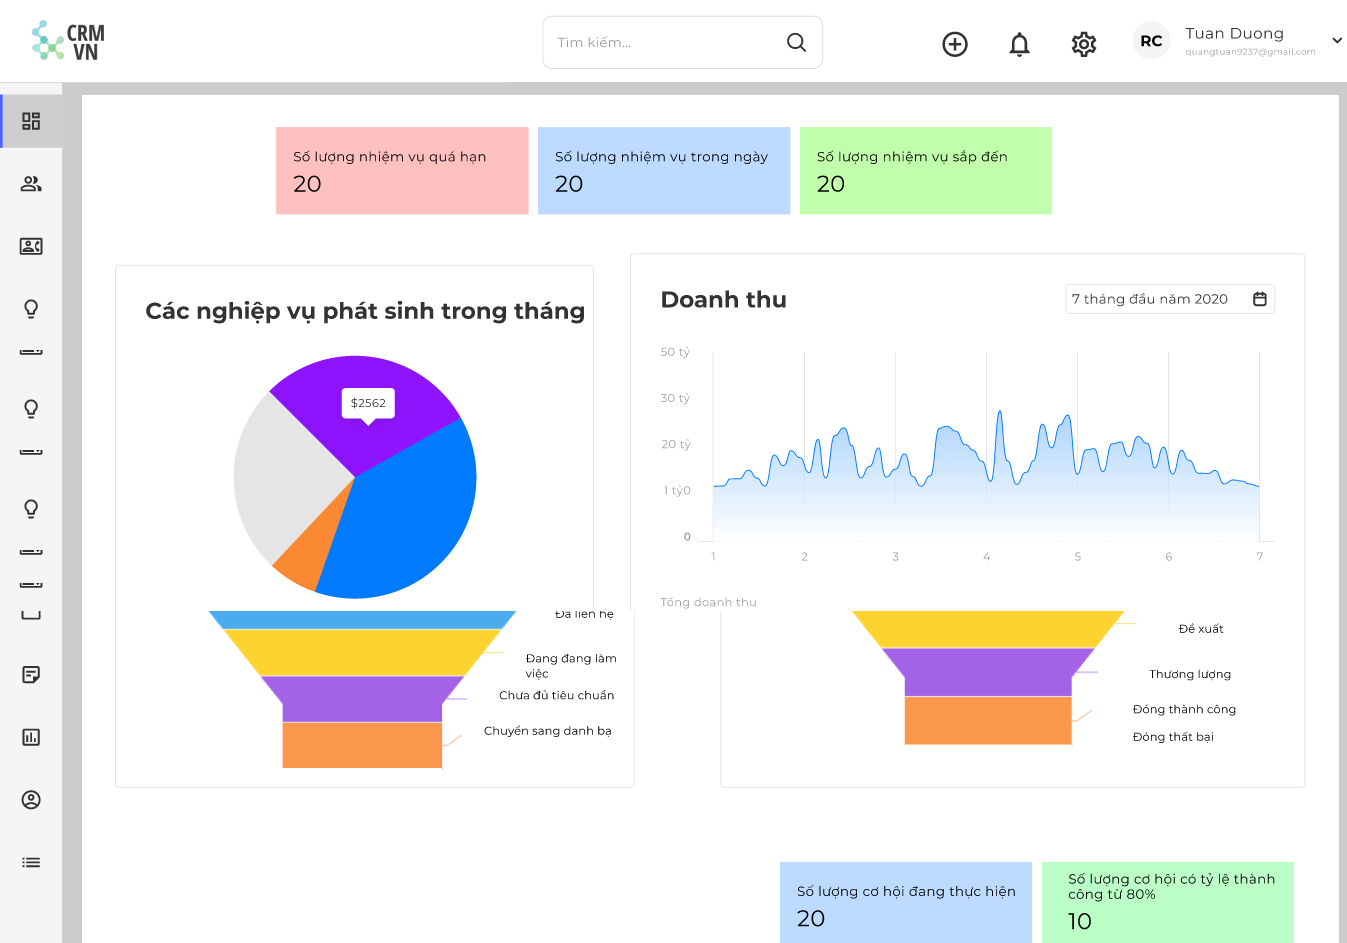
\includegraphics[width=\textwidth]{Img/Nguyet/dashboard.png}
            \vspace{0.5cm}
            \caption{Màn hình trang chủ}
            \label{trangchu}
        \end{figure}
        \item Tất cả \\
        Với tư cách người dùng, tôi hiển thị thanh menu trên tất cả các trang.
        \begin{itemize}
            \item Tìm kiếm toàn cục\\
            Với tư cách người dùng, tôi muốn tìm kiếm toàn cục các thông tin tại thanh menu để thuận tiện cho việc truy cập nhanh.
            \item Tạo mới nhanh các đối tượng \\
            Với tư cách người dùng, tôi muốn tạo mới các đối tượng một cách nhanh chóng tại trang chủ.
            \item Hiển thị thông báo \\
            Với tư cách người dùng, tôi muốn hiển thị thông báo trên thanh menu để dễ dàng nhận thấy.
            \item Hiển thị tên và ảnh đại diện \\
            Với tư cách người dùng, tôi muốn hiển thị tên và ảnh đại diện của người dùng lên thanh menu.
            \item Xem thông tin cá nhân \\
            Với tư cách người dùng, tôi muốn xem thông tin cá nhân để dễ dàng cập nhật khi có thay đổi.
            \item Truy cập trang cài đặt \\
            Với tư cách người dùng, tôi muốn truy cập đến trang cài đặt để thiết lập một số thông tin cho tài khoản.
        \end{itemize}
        \begin{figure}[H]
            \centering 
\includegraphics[width=\textwidth]{Img/Nguyet/all.png}
            \vspace{0.5cm}
            \caption{Màn hình thanh menu}
            \label{menu}
        \end{figure}


        \item Trang tiềm năng \\
        Với tư cách người dùng, tôi muốn quản lý tiềm năng để chăm sóc và triển khai các chiến dịch phù hợp.
        \begin{itemize}
            \item Xem danh sách tiềm năng \\
            Với tư cách người dùng, tôi muốn xem danh sách tất cả các tiềm năng để có cái nhìn tổng quan về tiềm năng.
            \begin{figure}[H]
                \centering 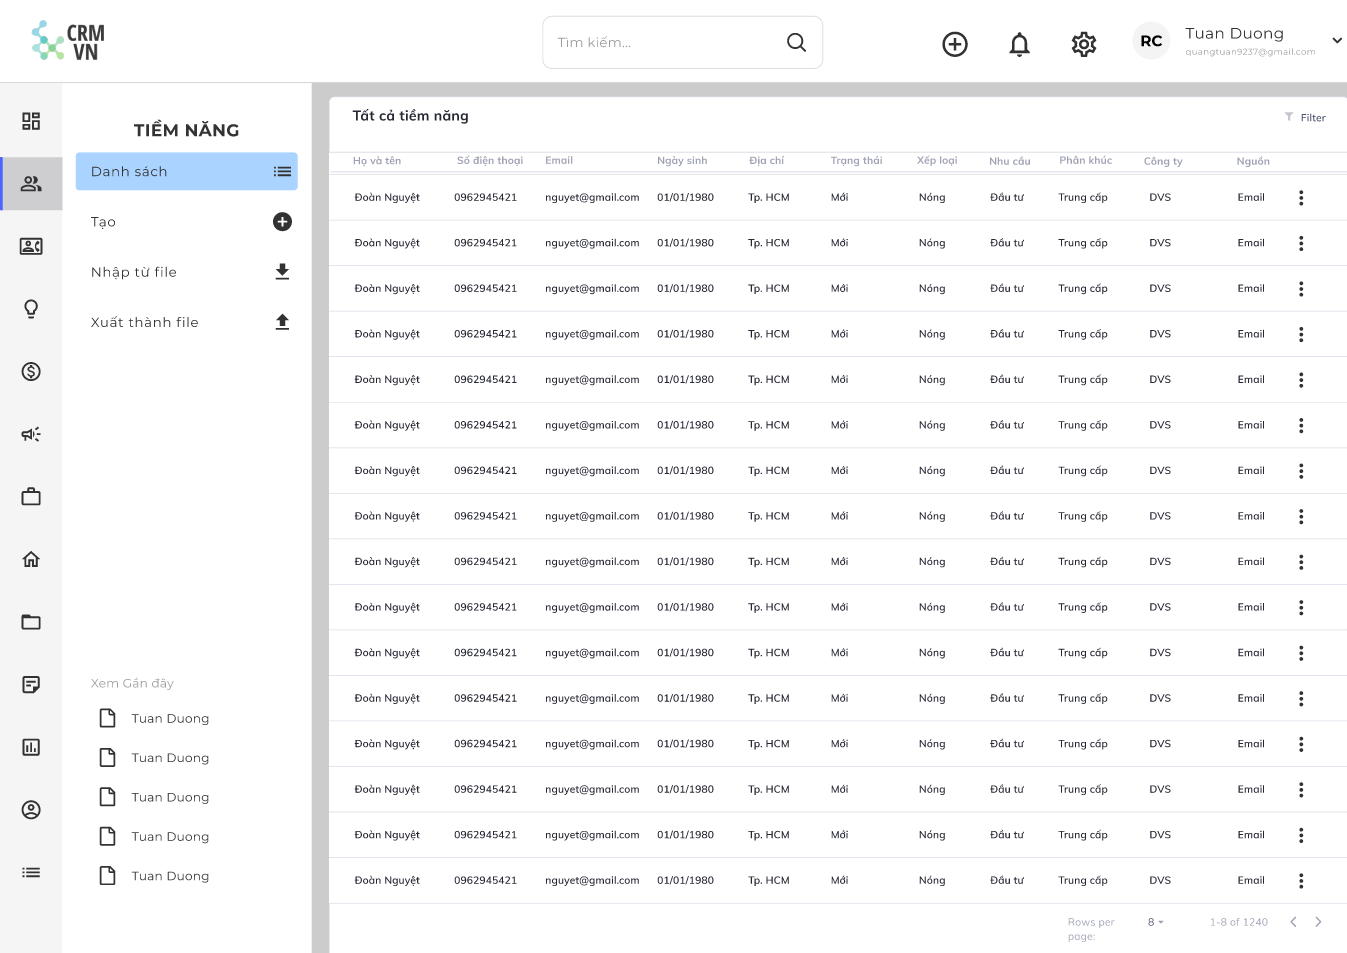
\includegraphics[width=\textwidth]{Img/Nguyet/dstiemnang.png}
                \vspace{0.5cm}
                \caption{Màn hình xem danh sách tiềm năng}
                \label{dstiemnang}
            \end{figure}
            \item Lọc thông tin tiềm năng \\
            Với tư cách người dùng, tôi muốn lọc danh sách tiềm năng theo các thuộc tính tùy chọn để dễ dàng chọn tiềm năng.

            \begin{figure}[H]
                \centering 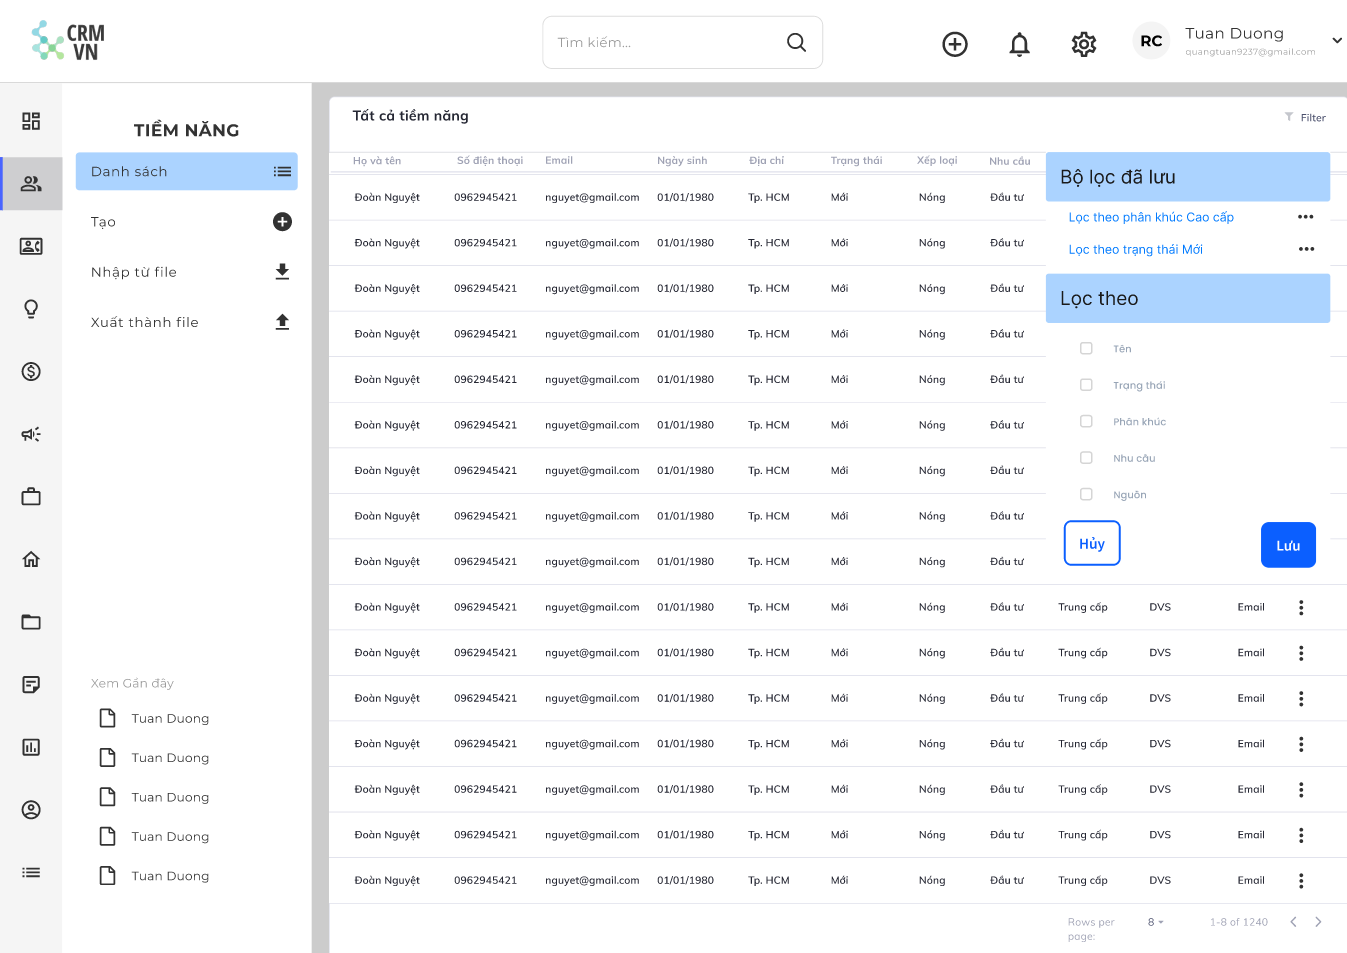
\includegraphics[width=\textwidth]{Img/Nguyet/loc.png}
                \vspace{0.5cm}
                \caption{Màn hình lọc thông tin tiềm năng}
                \label{loctiemnang}
            \end{figure}

            \item Tạo mới tiềm năng \\
            Với tư cách người dùng, tôi muốn tạo mới tiềm năng để quản lý.

            \begin{figure}[H]
                \centering 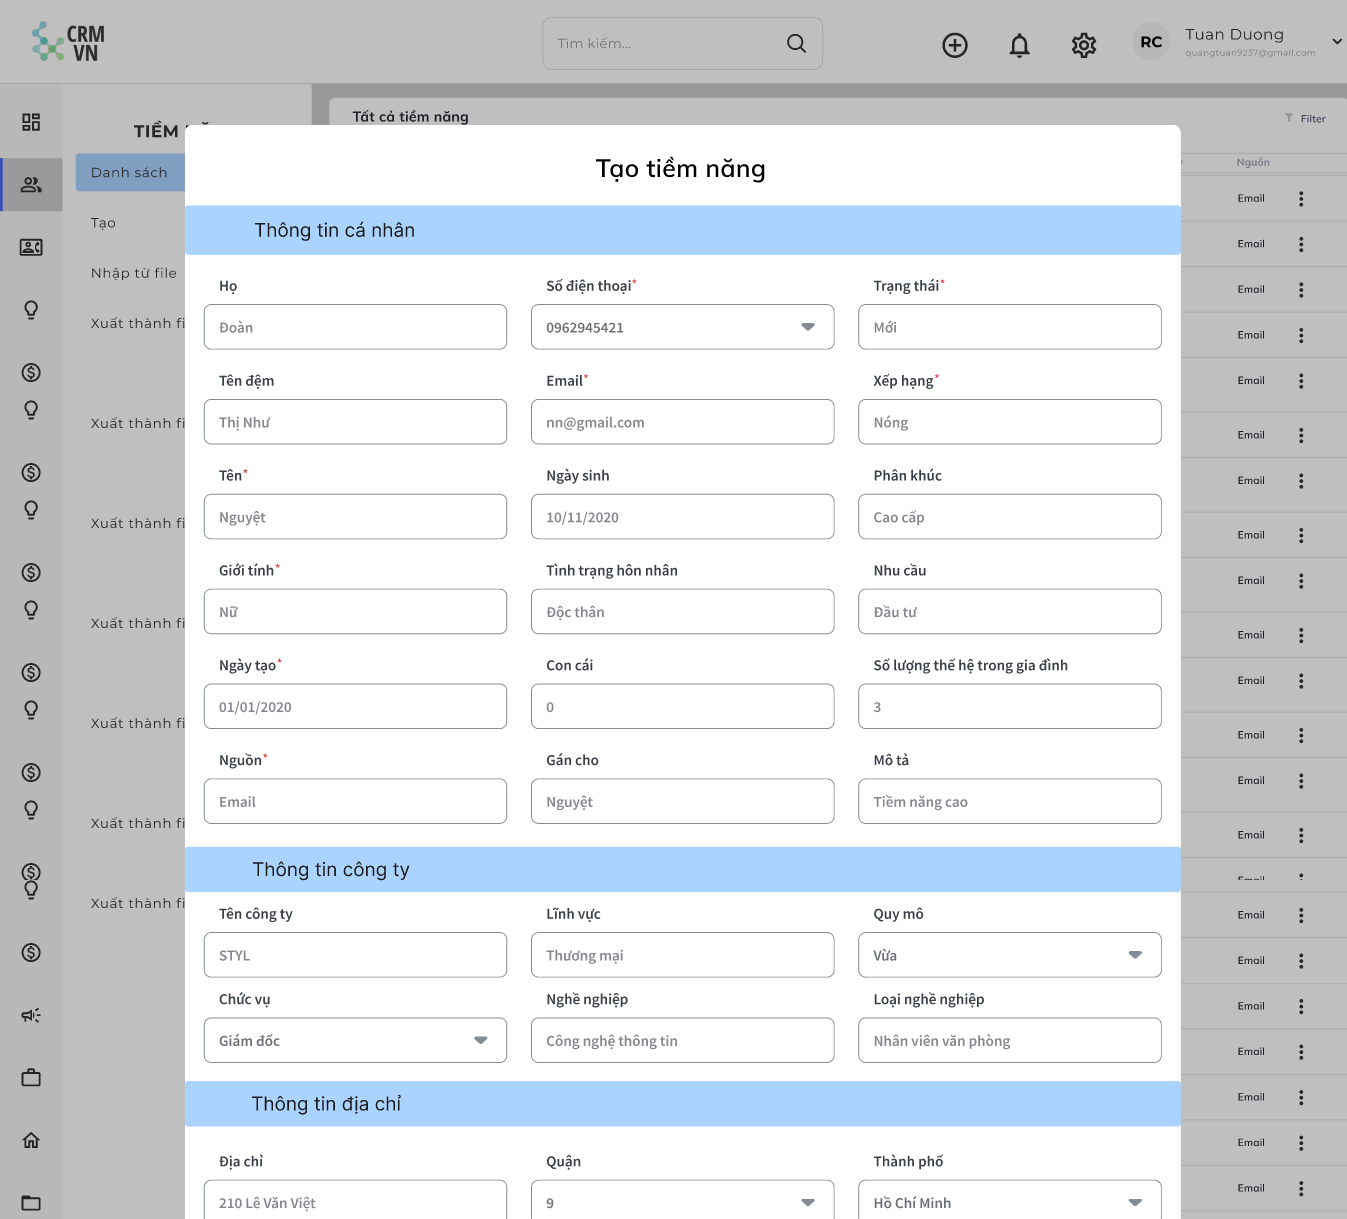
\includegraphics[width=\textwidth]{Img/Nguyet/taotiemnang.png}
                \vspace{0.5cm}
                \caption{Màn hình tạo tiềm năng}
                \label{taotiemnang}
            \end{figure}
            \item Xem chi tiết tiềm năng \\
            Với tư cách người dùng, tôi muốn xem chi tiết từng tiềm năng để lấy thông tin cần thiết.
            \begin{figure}[H]
                \centering 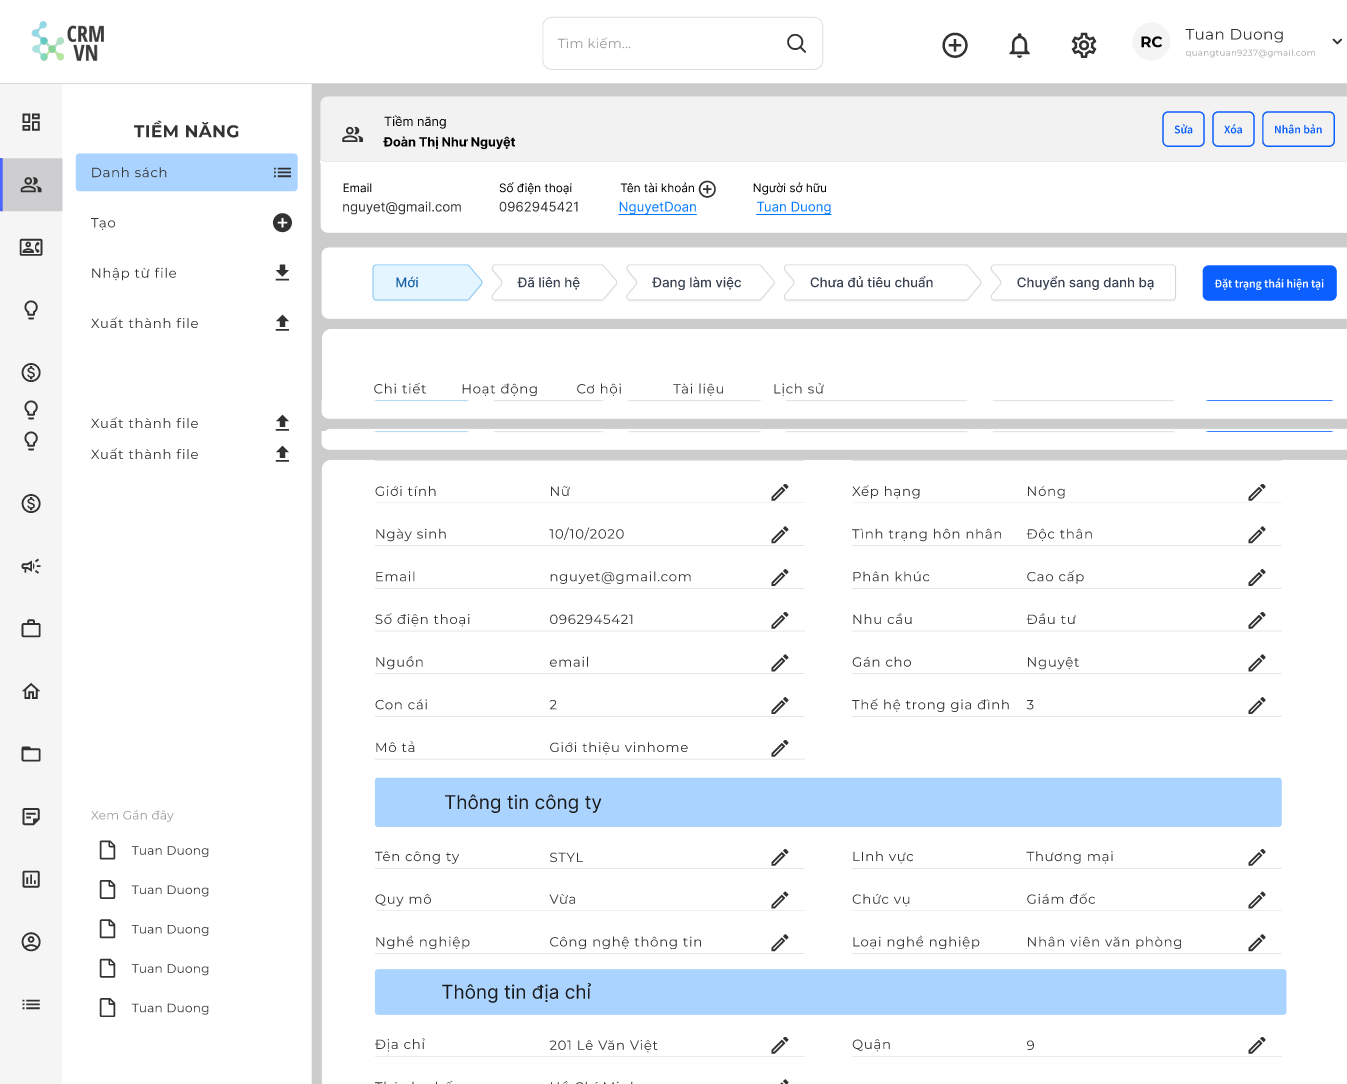
\includegraphics[width=\textwidth]{Img/Nguyet/chitiettiemnang.png}
                \vspace{0.5cm}
                \caption{Màn hình xem chi tiết tiềm năng}
                \label{chitiettiemnang}
            \end{figure}
            \item Sửa tiềm năng \\
            Với tư cách người dùng, tôi muốn sửa thông tin tiềm năng để cập nhật đúng thông tin.
            \begin{figure}[H]
                \centering 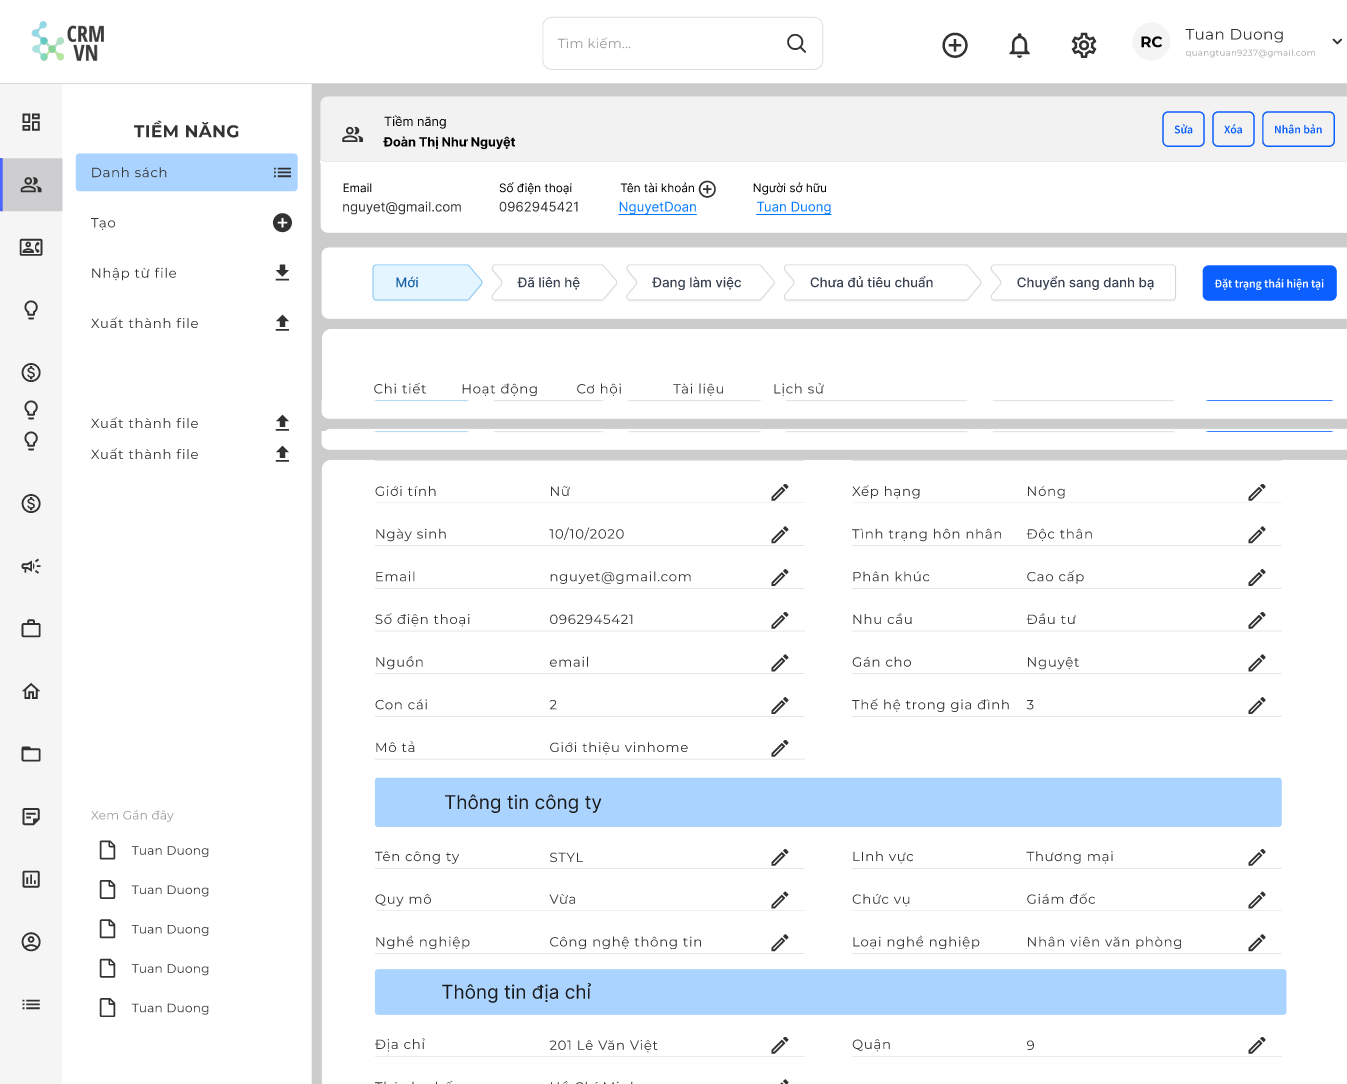
\includegraphics[width=\textwidth]{Img/Nguyet/chitiettiemnang.png}
                \vspace{0.5cm}
                \caption{Màn hình sửa tiềm năng}
                \label{suatiemnang}
            \end{figure}
            \item Xóa tiềm năng \\
            Với tư cách người dùng, tôi muốn xóa thông tin tiềm năng khi không cần thiết.
            \begin{figure}[H]
                \centering 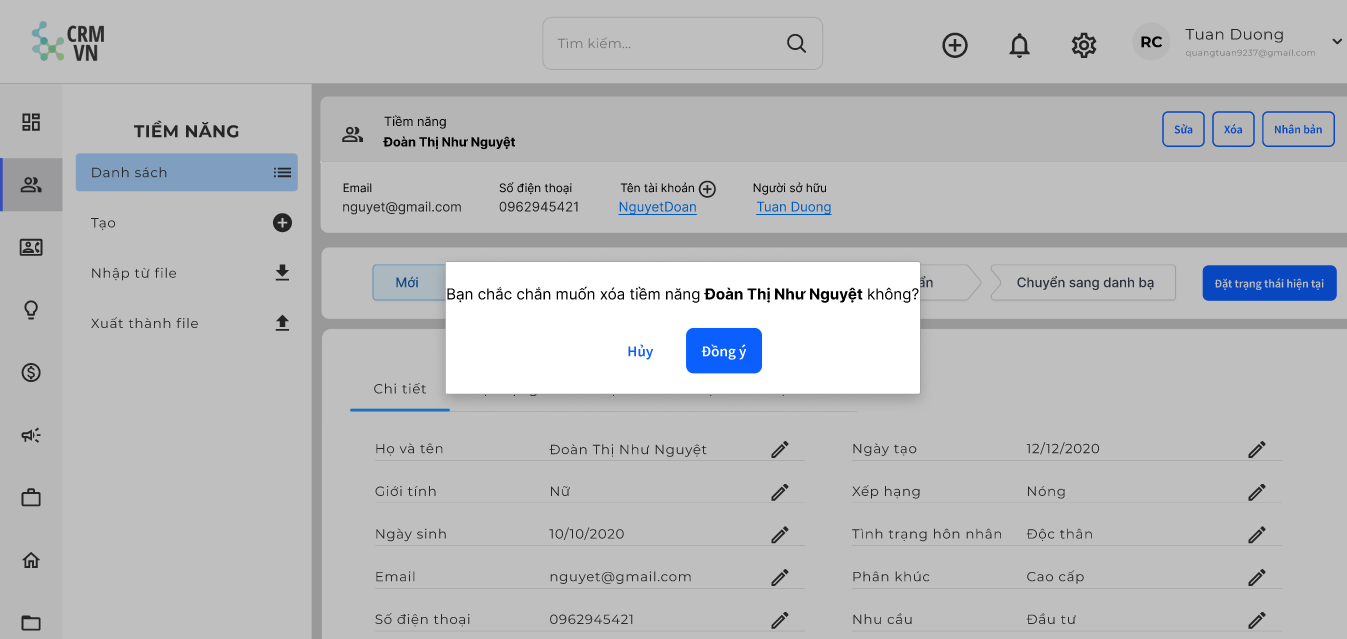
\includegraphics[width=\textwidth]{Img/Nguyet/xoatiemnang.png}
                \vspace{0.5cm}
                \caption{Màn hình xóa tiềm năng}
                \label{xoatiemnang}
            \end{figure}
            \item Nhân bản tiềm năng \\
            Với tư cách người dùng, tôi muốn nhân bản tiềm năng để thuận tiện cho việc tạo tiềm năng có thông tin gần giống.
            \begin{figure}[H]
                \centering 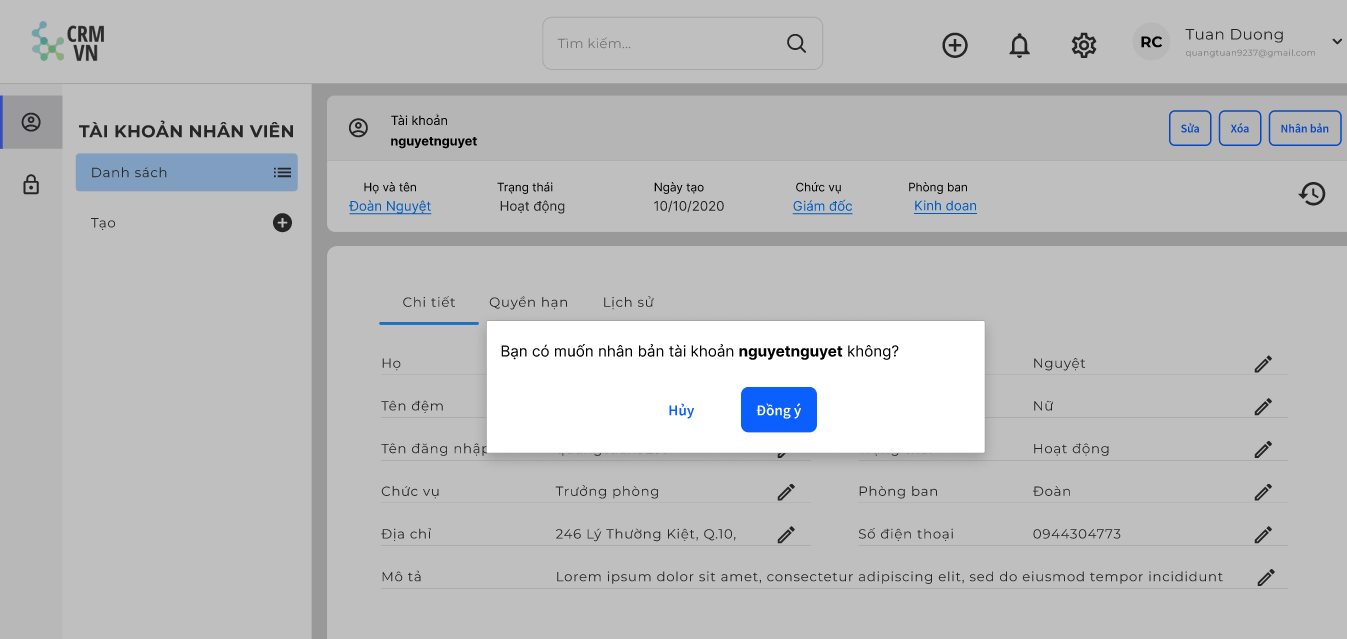
\includegraphics[width=\textwidth]{Img/Nguyet/nhanban.png}
                \vspace{0.5cm}
                \caption{Màn hình nhân bản tiềm năng}
                \label{nhanbantiemnang}
            \end{figure}
            \item Tạo tài khoản cho tiềm năng \\
            Với tư cách khách hàng, tôi muốn tạo tài khoản cho tiềm năng nếu tiềm năng này chưa có tài khoản và mong muốn tạo tài khoản.
            \begin{figure}[H]
                \centering 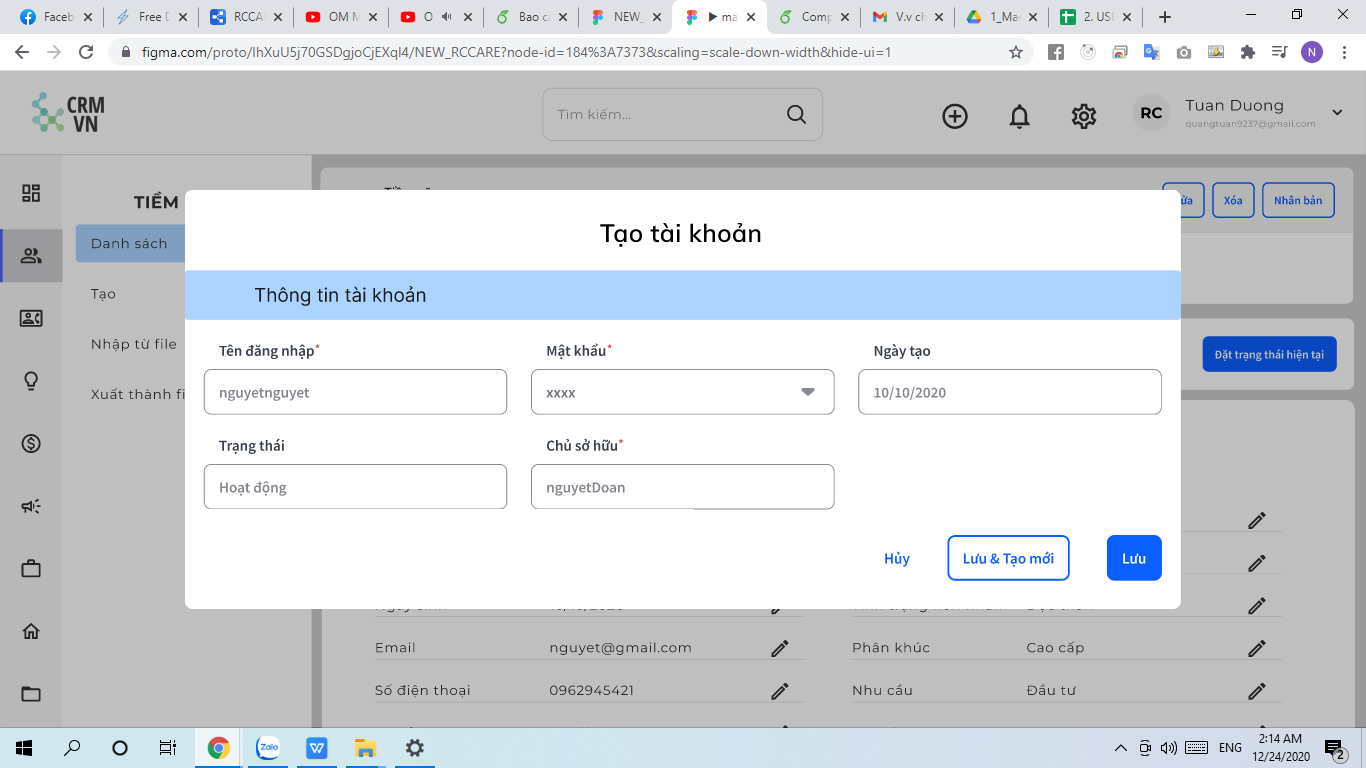
\includegraphics[width=\textwidth]{Img/Nguyet/taotktm.png}
                \vspace{0.5cm}
                \caption{Màn hình tạo tài khoản cho tiềm năng}
                \label{taotktiemnang}
            \end{figure}

            \item Chuyển đổi tiềm năng thành khách hàng \\
            Với tư cách người dùng, tôi muốn chuyển đổi tiềm năng thành khách hàng
            \begin{figure}[H]
                \centering 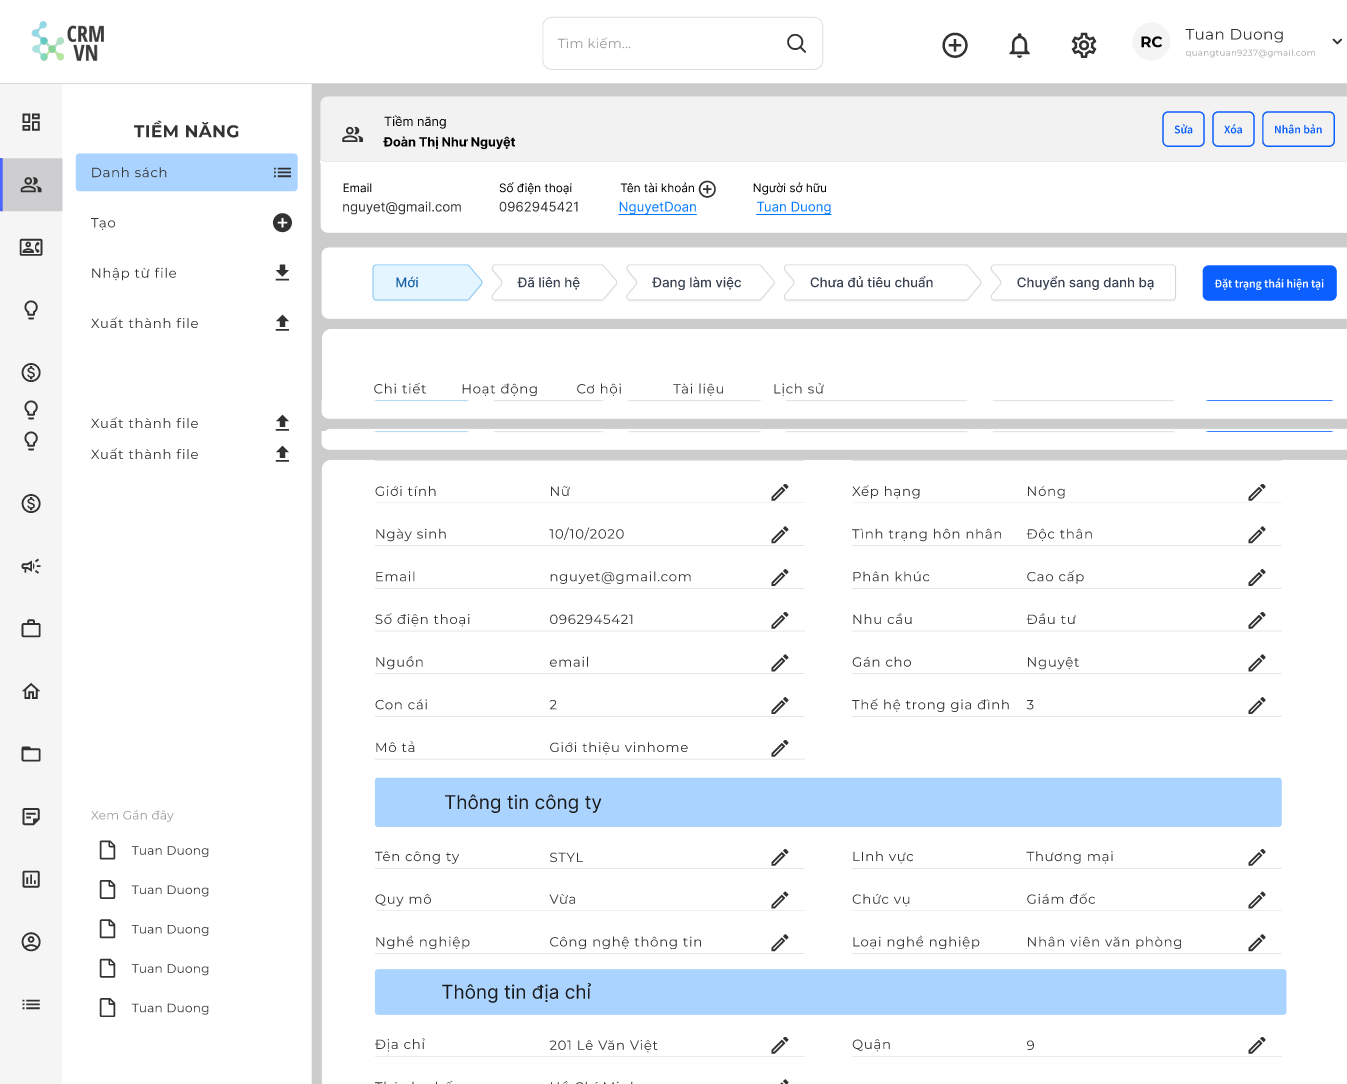
\includegraphics[width=\textwidth]{Img/Nguyet/chitiettiemnang.png}
                \vspace{0.5cm}
                \caption{Màn hình chuyển đổi tiềm năng thành khách hàng}
                \label{chuyenthanhkh}
            \end{figure}

            \item Tạo hoạt động cho tiềm năng \\
            Với tư cách người dùng, tôi muốn tạo hoạt động cho tiềm năng.
            \begin{figure}[H]
                \centering 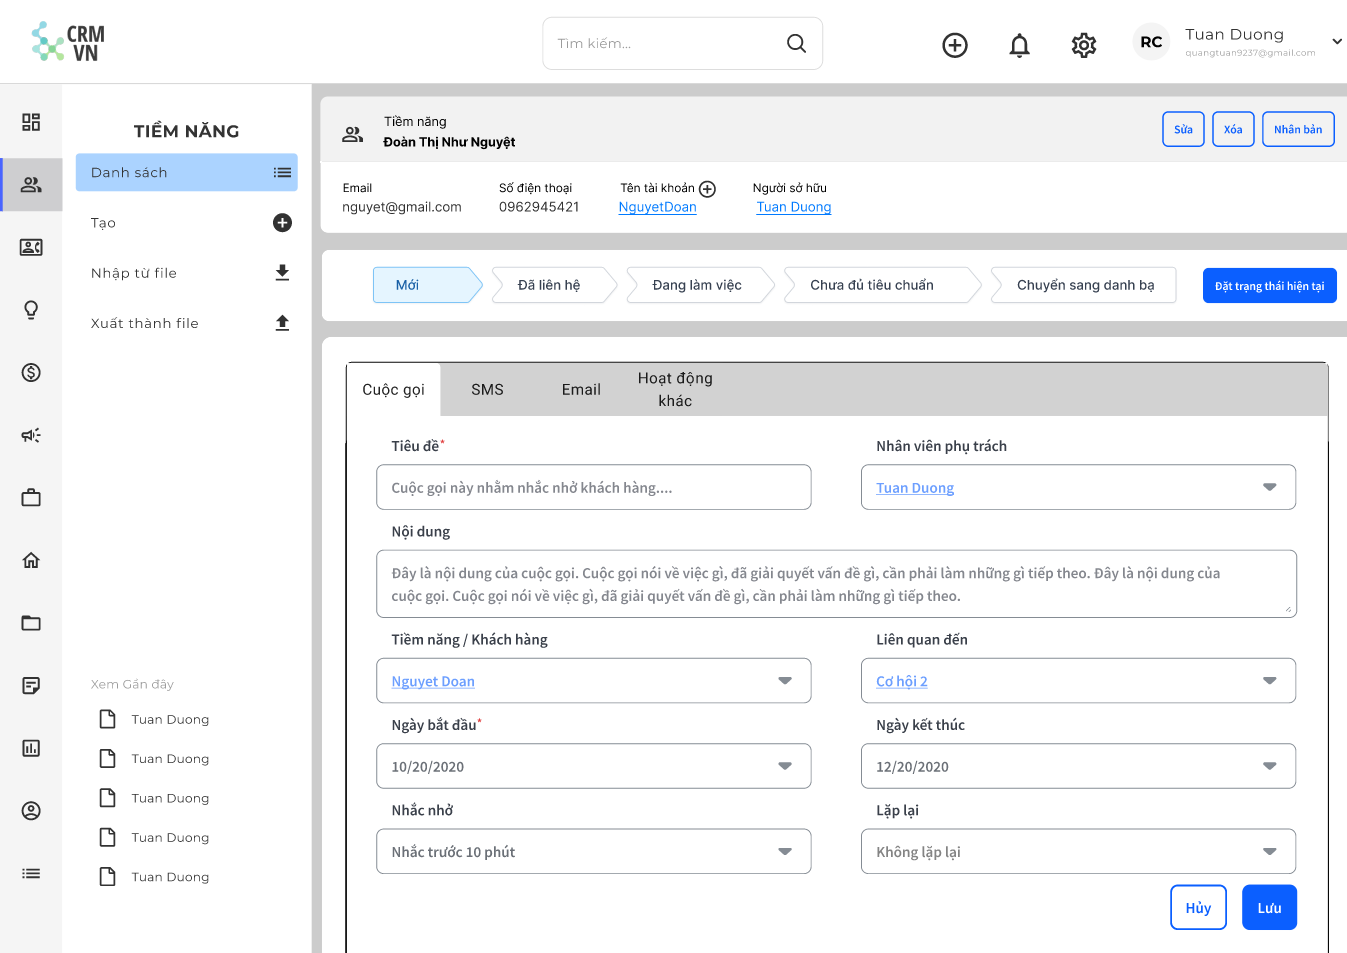
\includegraphics[width=\textwidth]{Img/Nguyet/hdcgoitn.png}
                \vspace{0.5cm}
                \caption{Màn hình tạo cuộc gọi}
                \label{goitn}
            \end{figure}

            \begin{figure}[H]
                \centering 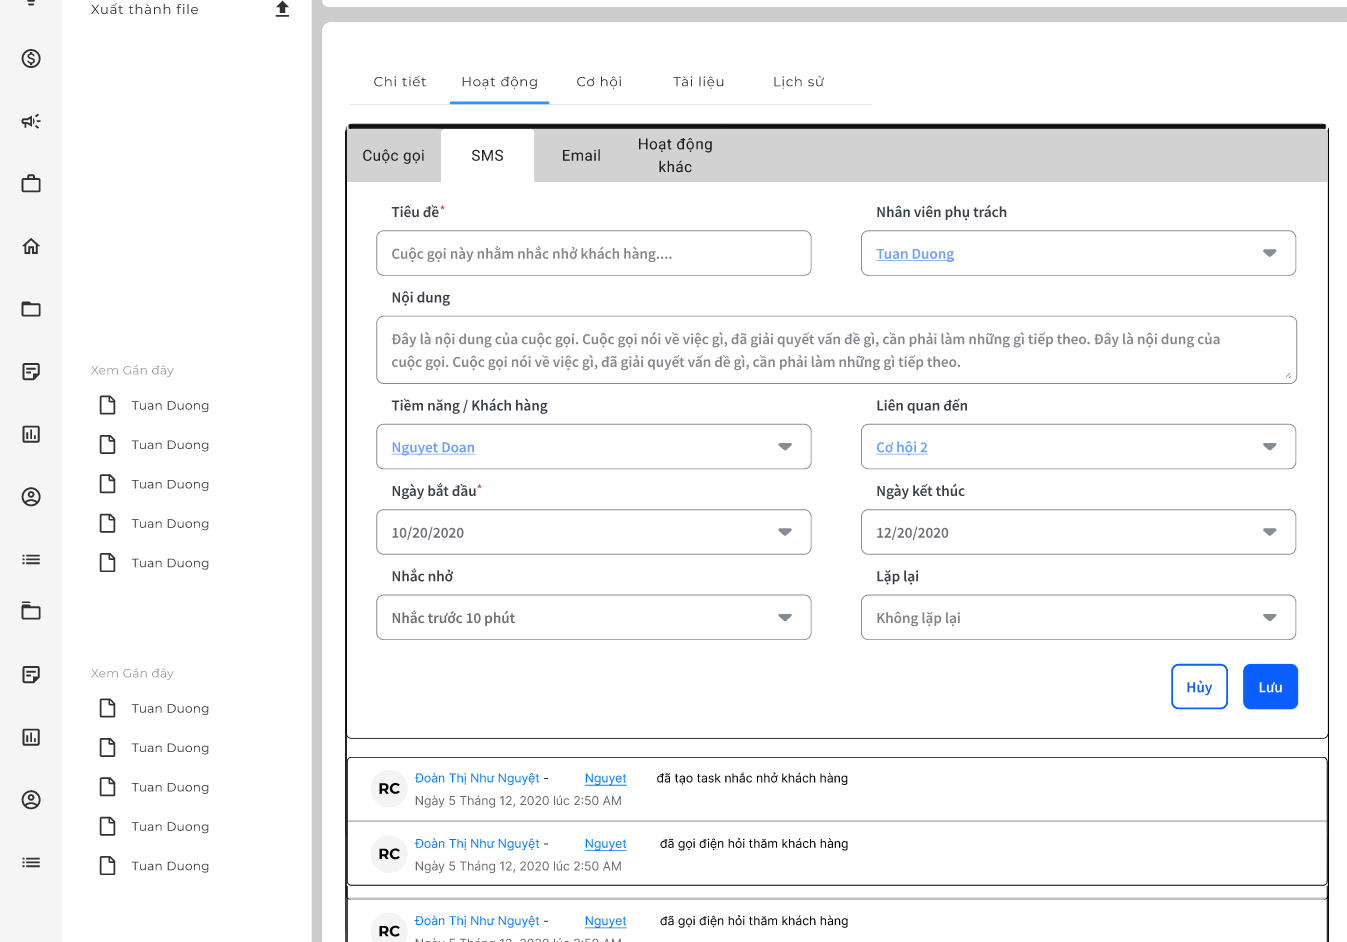
\includegraphics[width=\textwidth]{Img/Nguyet/smstn.png}
                \vspace{0.5cm}
                \caption{Màn hình tạo SMS cho tiềm năng}
                \label{smstn}
            \end{figure}

            \begin{figure}[H]
                \centering 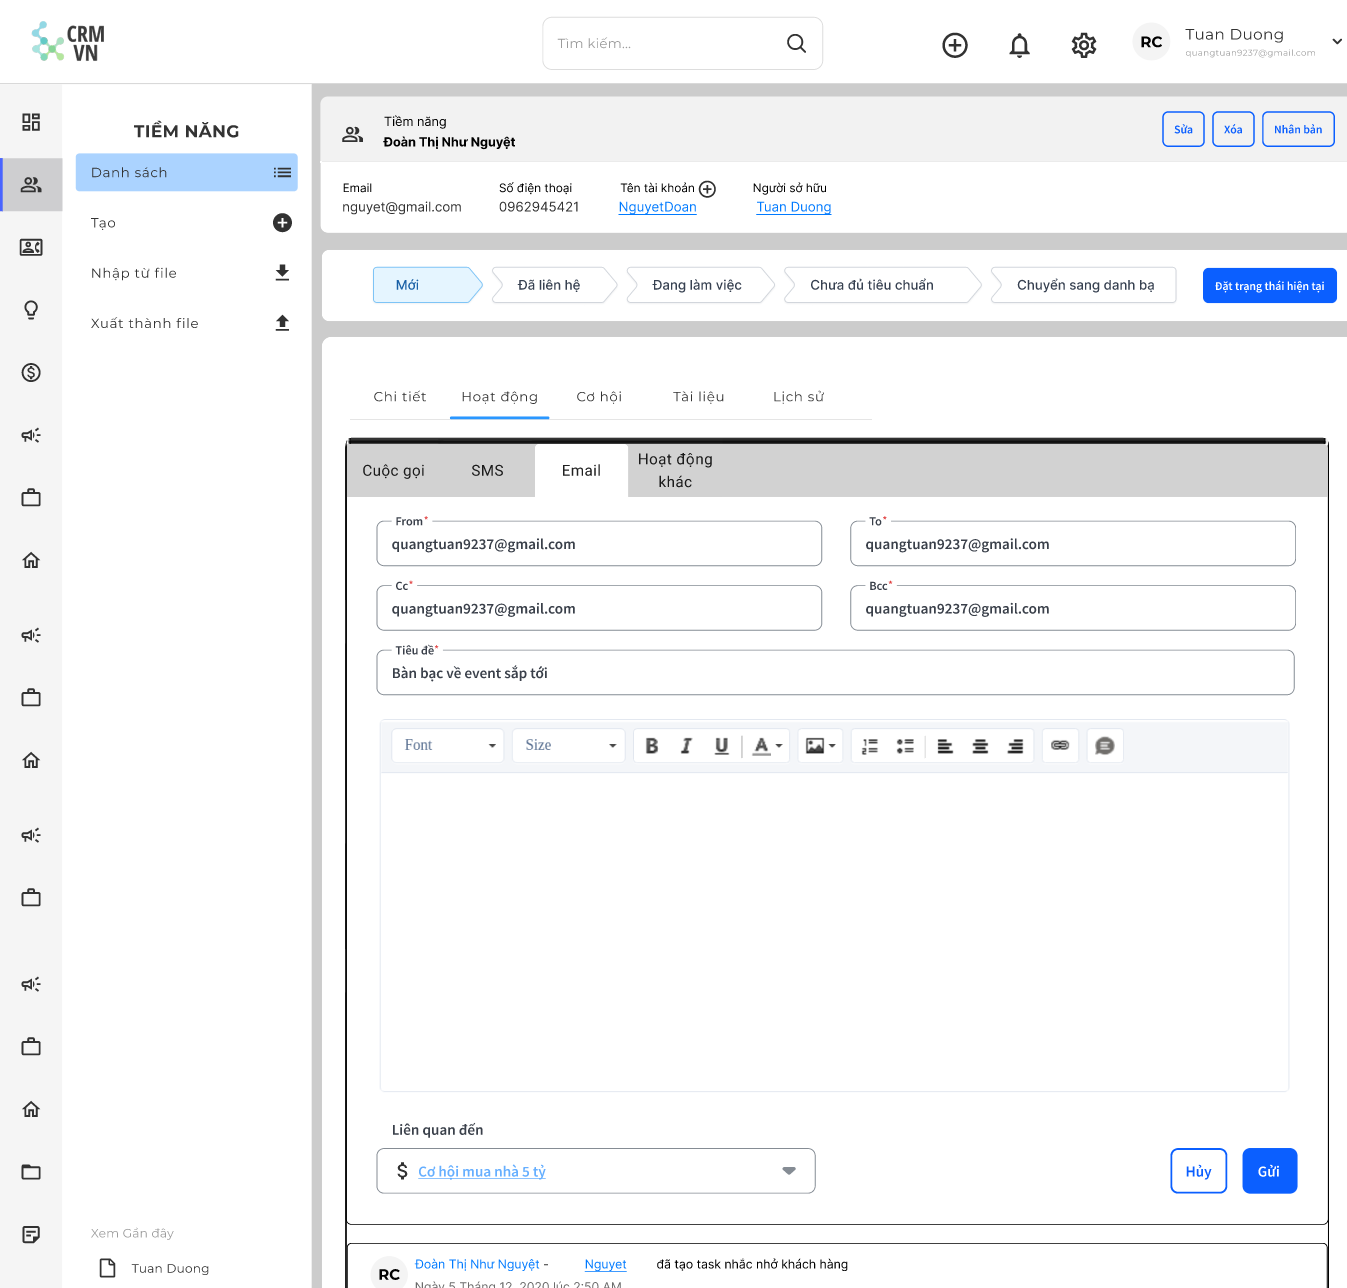
\includegraphics[width=\textwidth]{Img/Nguyet/emailtn.png}
                \vspace{0.5cm}
                \caption{Màn hình tạo email cho tiềm năng}
                \label{emailtn}
            \end{figure}


            \begin{figure}[H]
                \centering 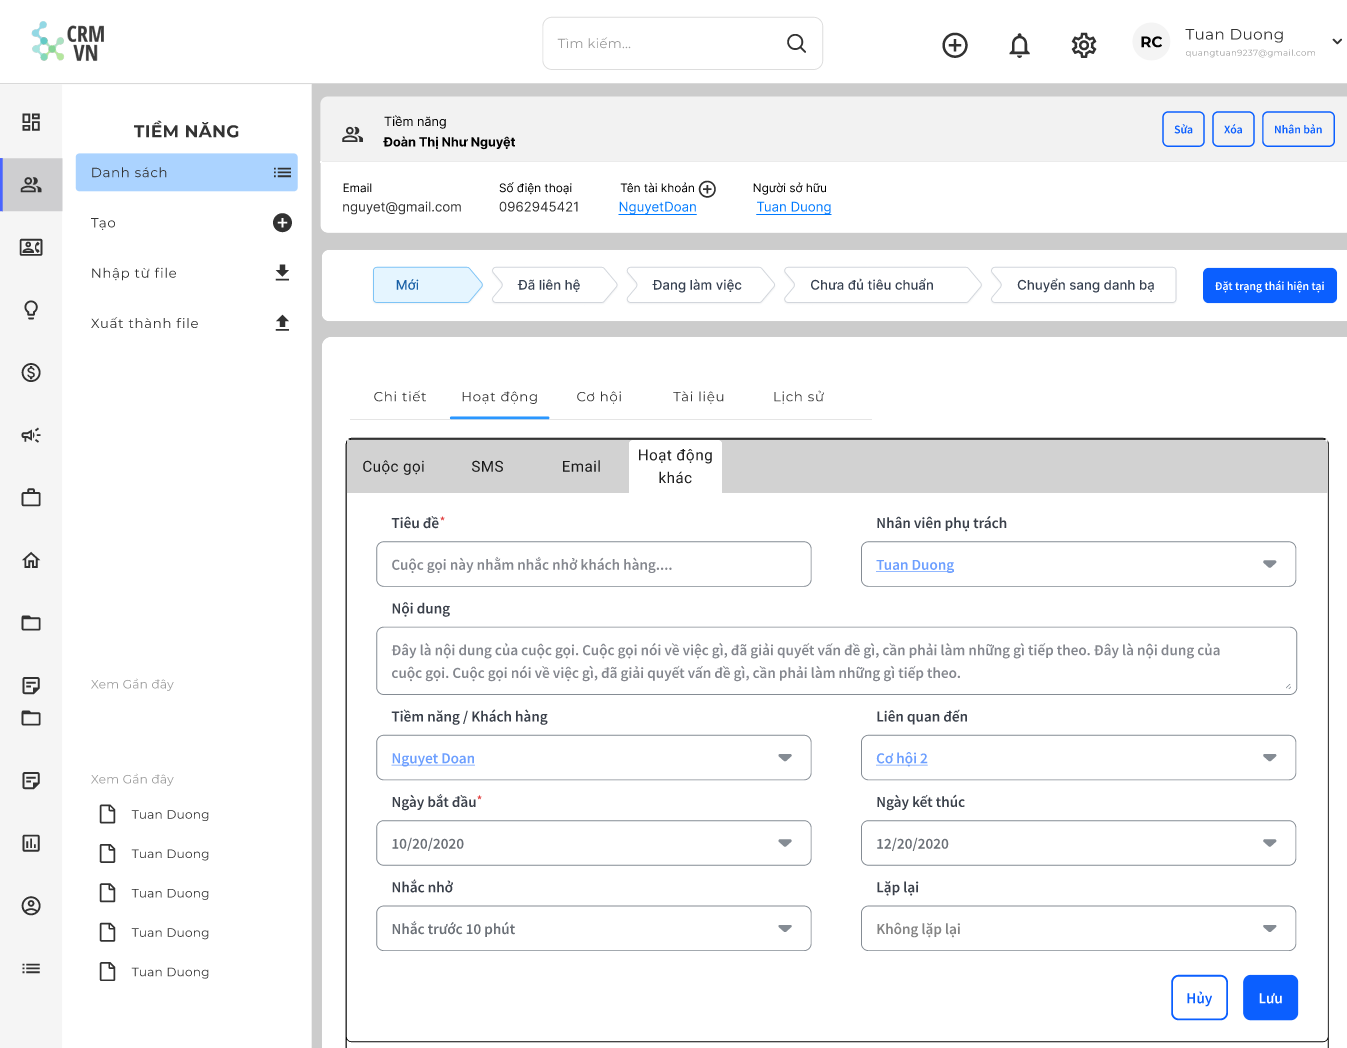
\includegraphics[width=\textwidth]{Img/Nguyet/tnhdkhac.png}
                \vspace{0.5cm}
                \caption{Màn hình tạo hoạt động khác cho tiềm năng}
                \label{hdkhactn}
            \end{figure}


            \item Xem danh sách các hoạt động đã thực hiện cho từng tiềm năng \\
            Với tư cách người dùng, tôi muốn xem danh sách các hoạt động đã thực hiện cho tường tiềm năng.
            \begin{figure}[H]
                \centering 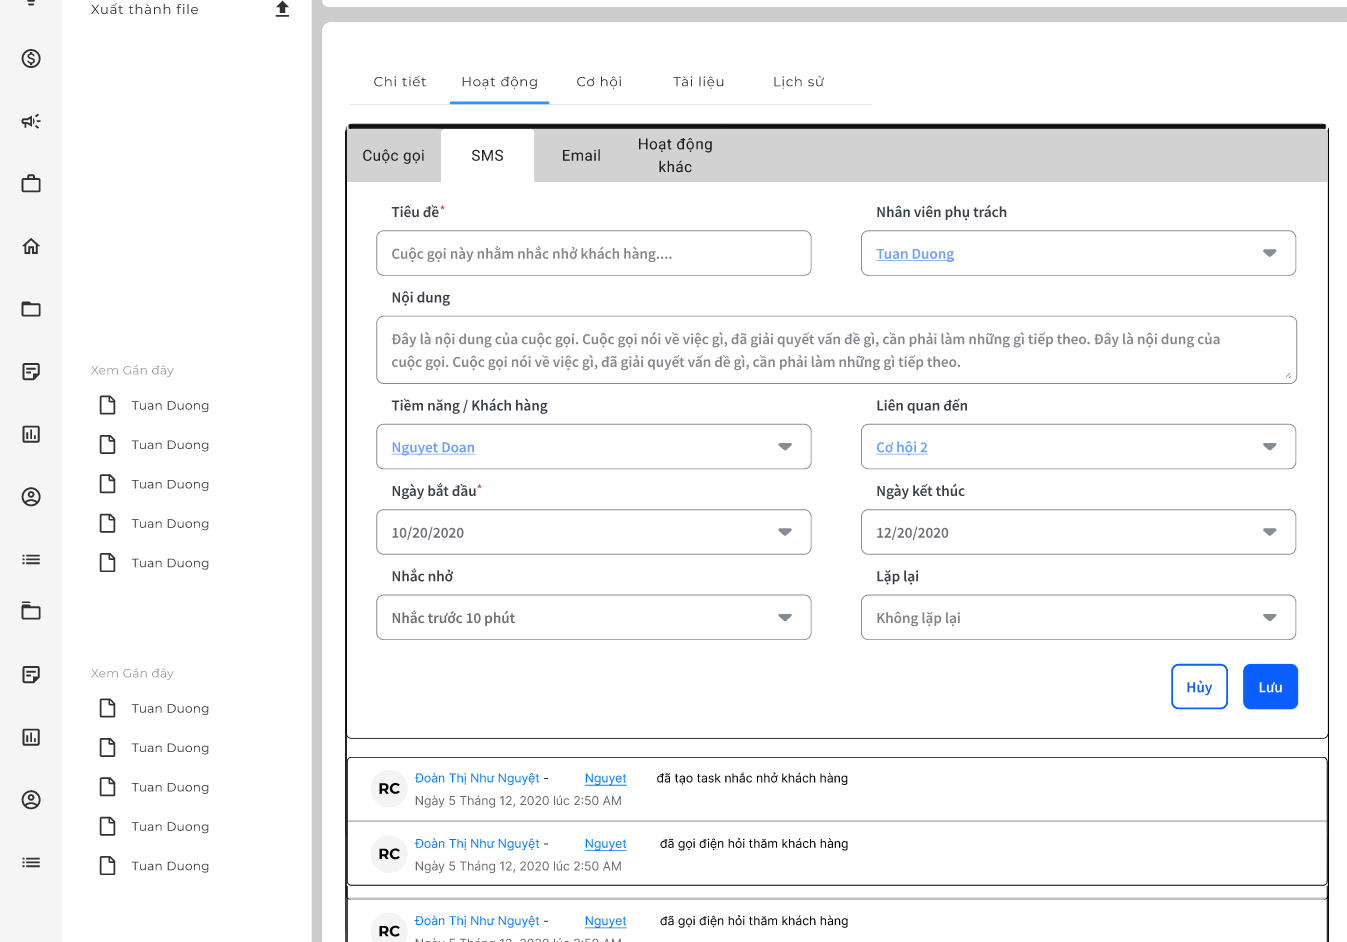
\includegraphics[width=\textwidth]{Img/Nguyet/smstn.png}
                \vspace{0.5cm}
                \caption{Màn hình xem danh sách các hoạt động đã thực hiện cho từng tiềm năng}
                \label{hdtn}
            \end{figure}
            \item Tạo cơ hội cho tiềm năng \\
            Với tư cách người dùng, tôi muốn tạo cơ hội cho tiềm năng để khoanh vùng đối tượng và có các kế hoạch chăm sóc cụ thể.

            \begin{figure}[H]
                \centering 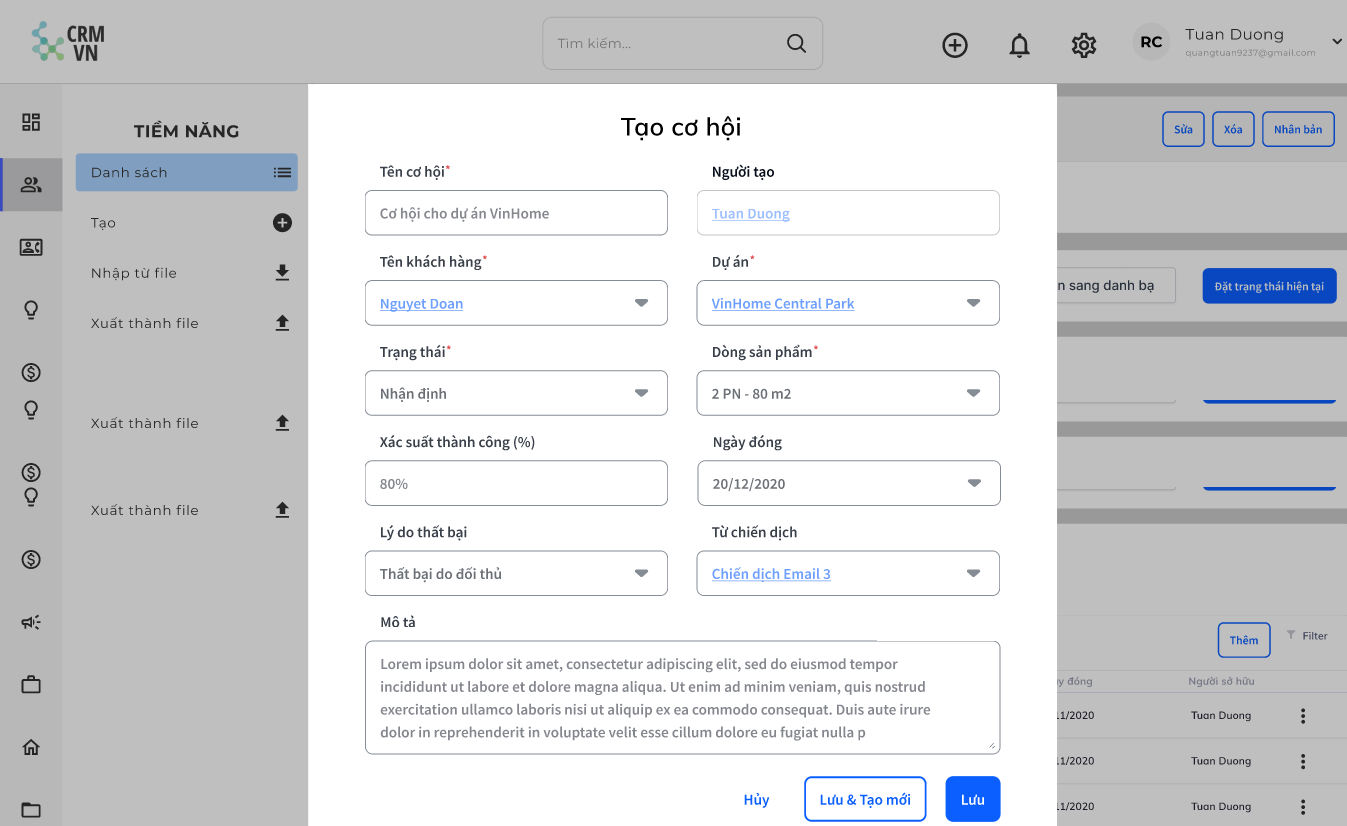
\includegraphics[width=\textwidth]{Img/Nguyet/taocohoitn.png}
                \vspace{0.5cm}
                \caption{Màn hình tạo cơ hội cho từng tiềm năng}
                \label{taocohoi}
            \end{figure}

            \item Xem danh sách cơ hội theo tiềm năng \\
            Với tư cách người dùng, tôi muốn xem danh sách cơ hội theo từng tiềm năng để đánh giá tổng quan về tiềm năng.

            \begin{figure}[H]
                \centering 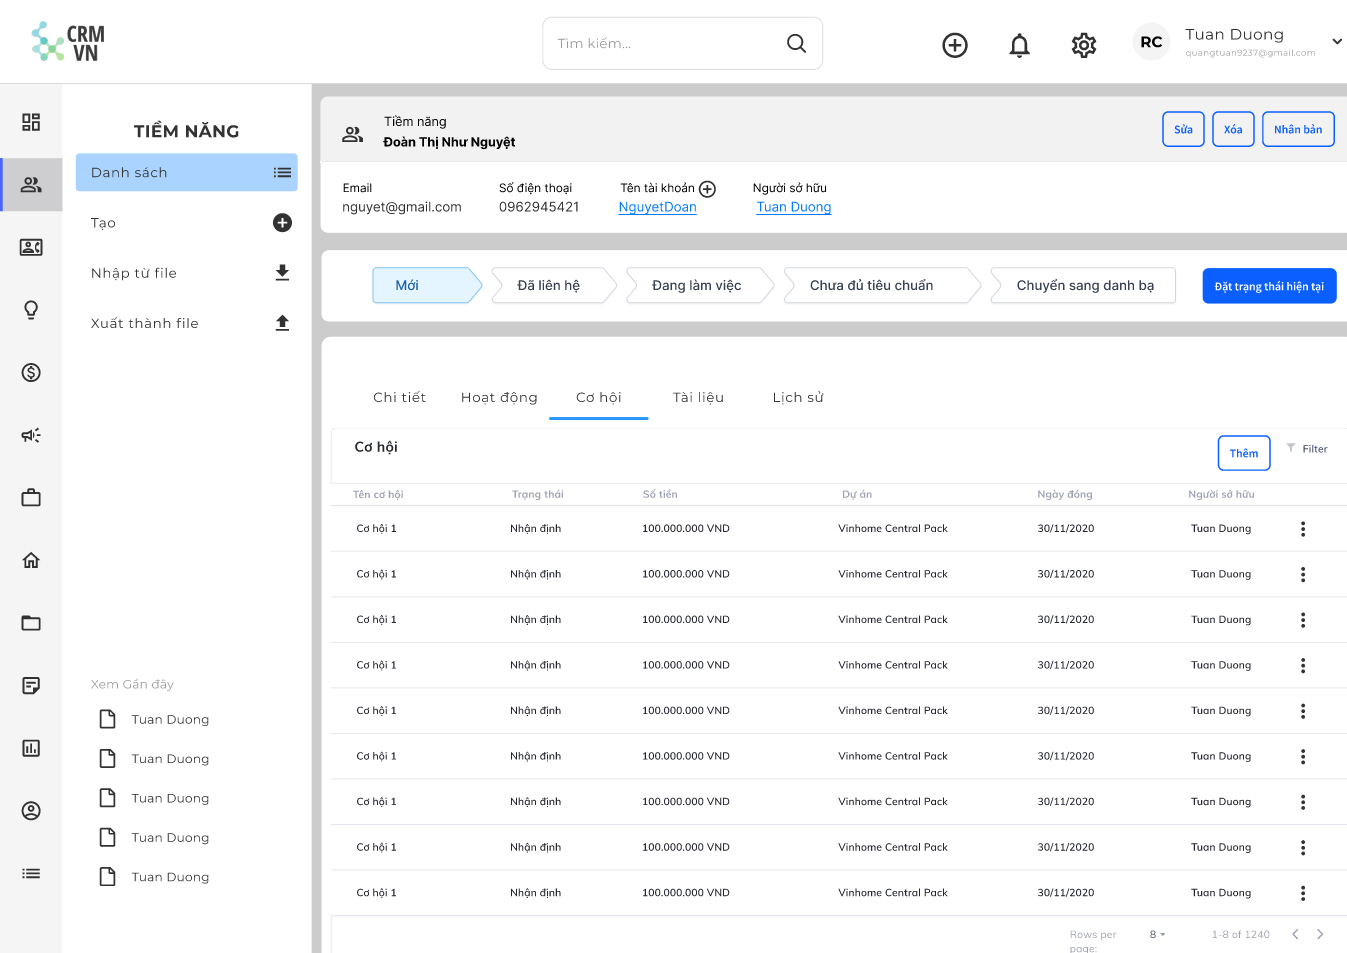
\includegraphics[width=\textwidth]{Img/Nguyet/dscntm.png}
                \vspace{0.5cm}
                \caption{Màn hình xem danh sách cơ hội theo từng tiềm năng}
                \label{dschtn}
            \end{figure}


            \item Xem chi tiết từng cơ hội theo tiềm năng \\
            Với tư cách người dùng, tôi muốn xem chi tiết từng cơ hội theo tiềm năng.

            \begin{figure}[H]
                \centering 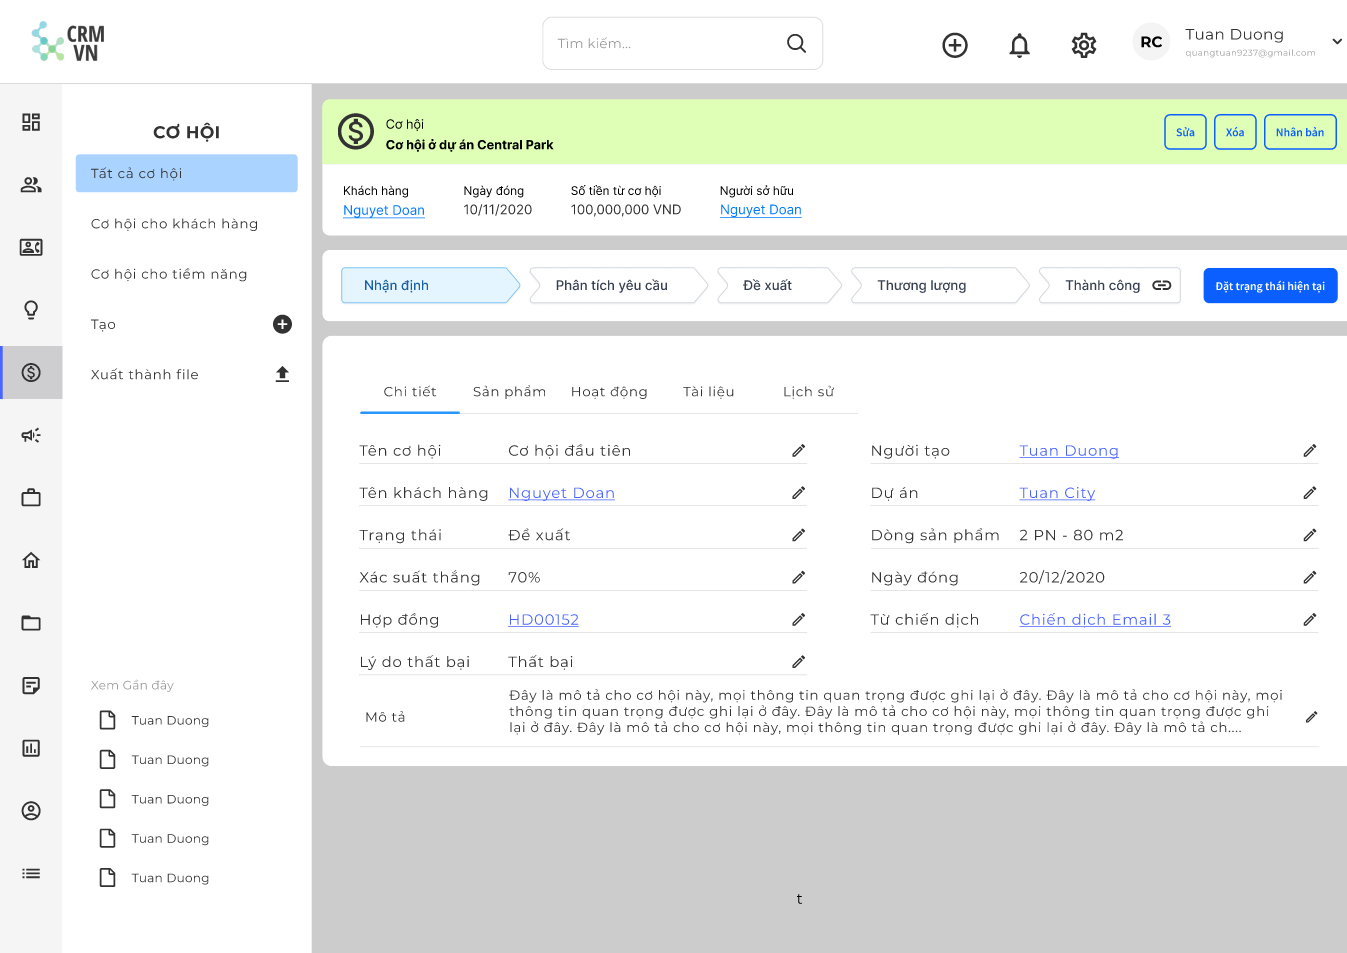
\includegraphics[width=\textwidth]{Img/Nguyet/chitietcohoi.png}
                \vspace{0.5cm}
                \caption{Màn hình xem chi tiết cơ hội theo tiềm năng}
                \label{chitietcohoi}
            \end{figure}

            \item Xem danh sách tài liệu đính kèm cho tiềm năng \\
            Với tư cách người dùng, tôi muốn xem danh sách tài liệu đính kèm cho tiềm năng.

            \begin{figure}[H]
                \centering 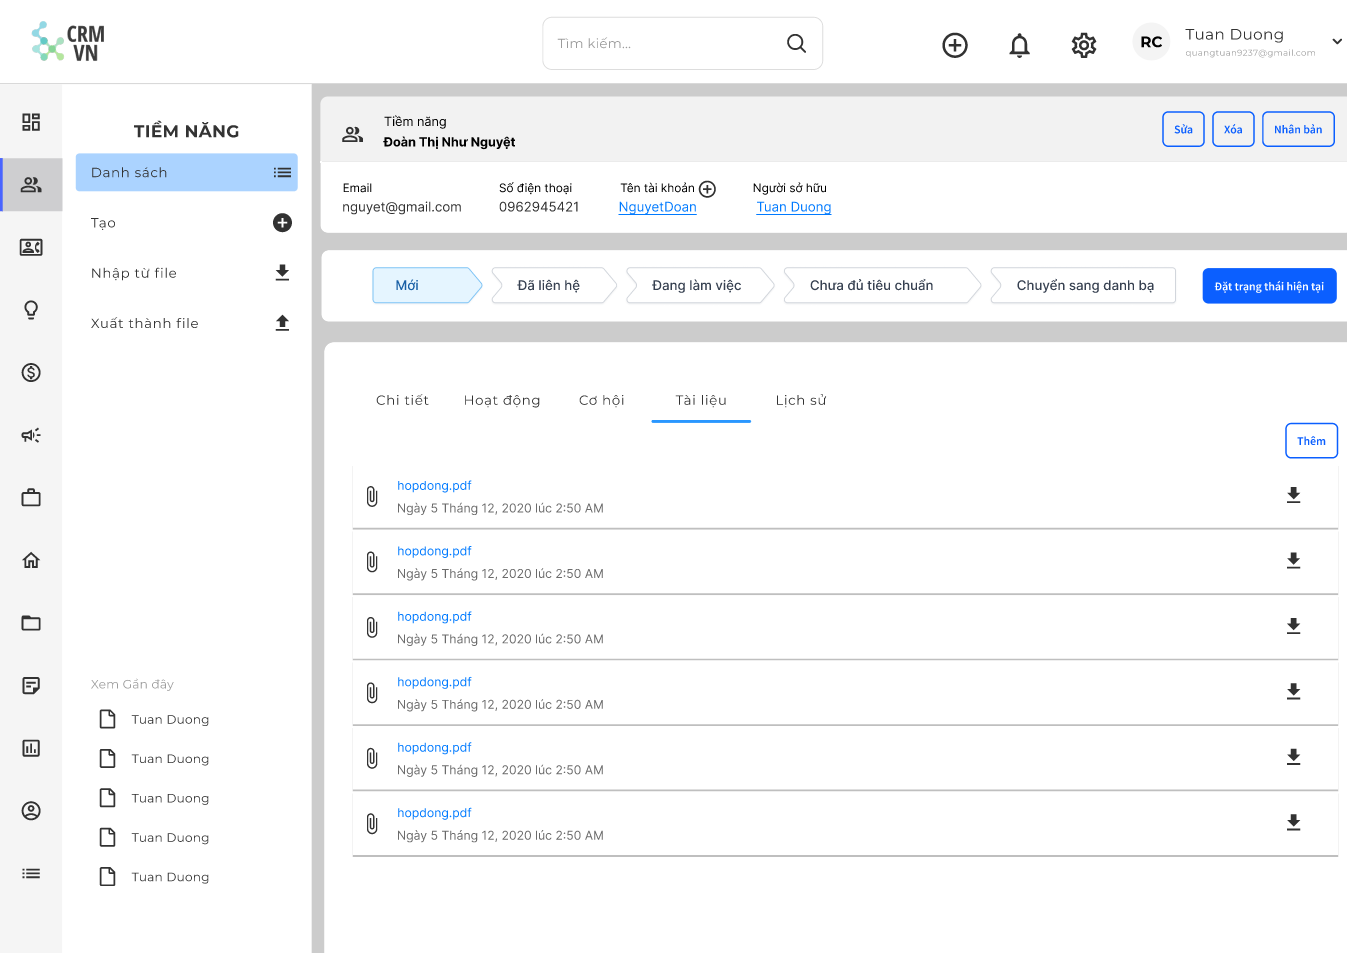
\includegraphics[width=\textwidth]{Img/Nguyet/danhsachtailieu.png}
                \vspace{0.5cm}
                \caption{Màn hình xem danh sách tài liệu đính kèm cho tiềm năng}
                \label{danhsachtailieu}
            \end{figure}

            \item  Thêm tài liệu cho tiềm năng \\
            Với tư cách người dùng, tôi muốn thêm tài liệu cho tiềm năng để lưu trữ.

            \begin{figure}[H]
                \centering 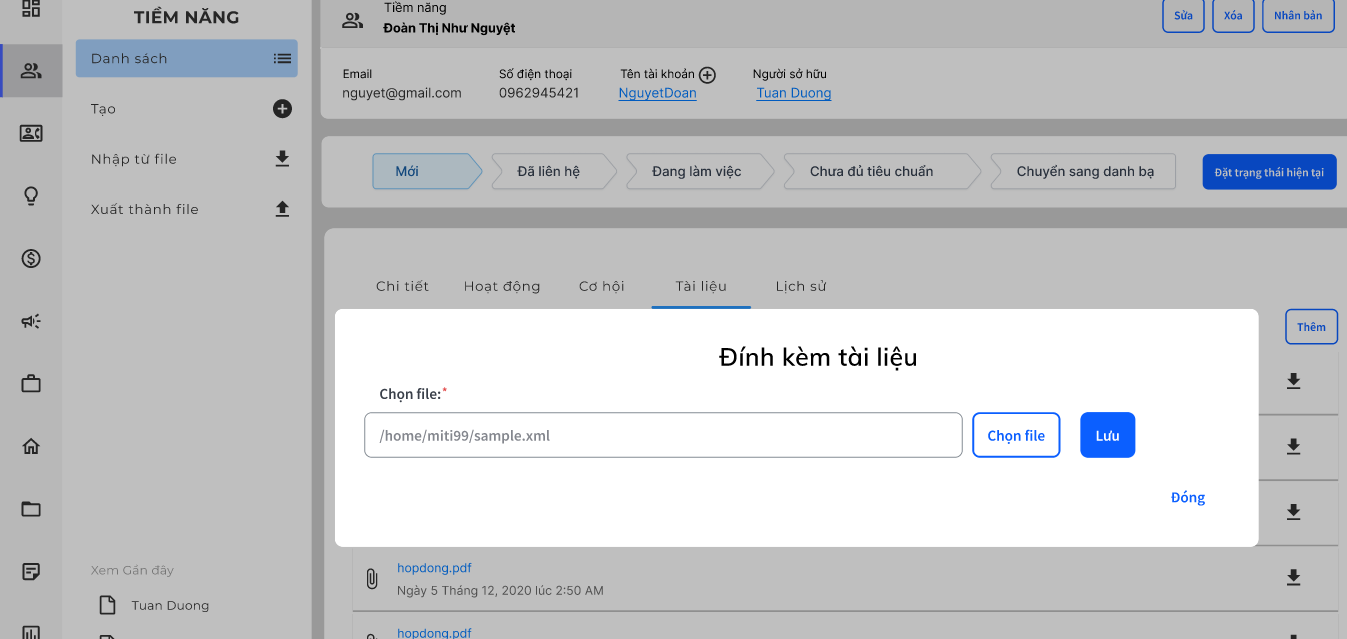
\includegraphics[width=\textwidth]{Img/Nguyet/dinhkemtailieutn.png}
                \vspace{0.5cm}
                \caption{Màn hình thêm tài liệu cho tiềm năng}
                \label{dinhkemtailieu}
            \end{figure}


            \item Sửa tài liệu cho tiềm năng \\
            Với tư cách người dùng, tôi muốn sửa tài liệu cho tiềm năng.
            \item Xóa tài liệu cho tiềm năng \\
            Với tư cách người dùng, tôi muốn xóa tài liệu đã đính kèm cho tiềm năng.
            \item Tải tài liệu theo từng tiềm năng \\
            Với tư cách người dùng, tôi muốn tải tài liệu đã đính kèm.
            \item Xem lịch sử thay đổi theo từng tiềm năng \\
            Với tư cách người dùng, tôi muốn xem lịch sử thay đổi theo từng tiềm năng.

            \begin{figure}[H]
                \centering 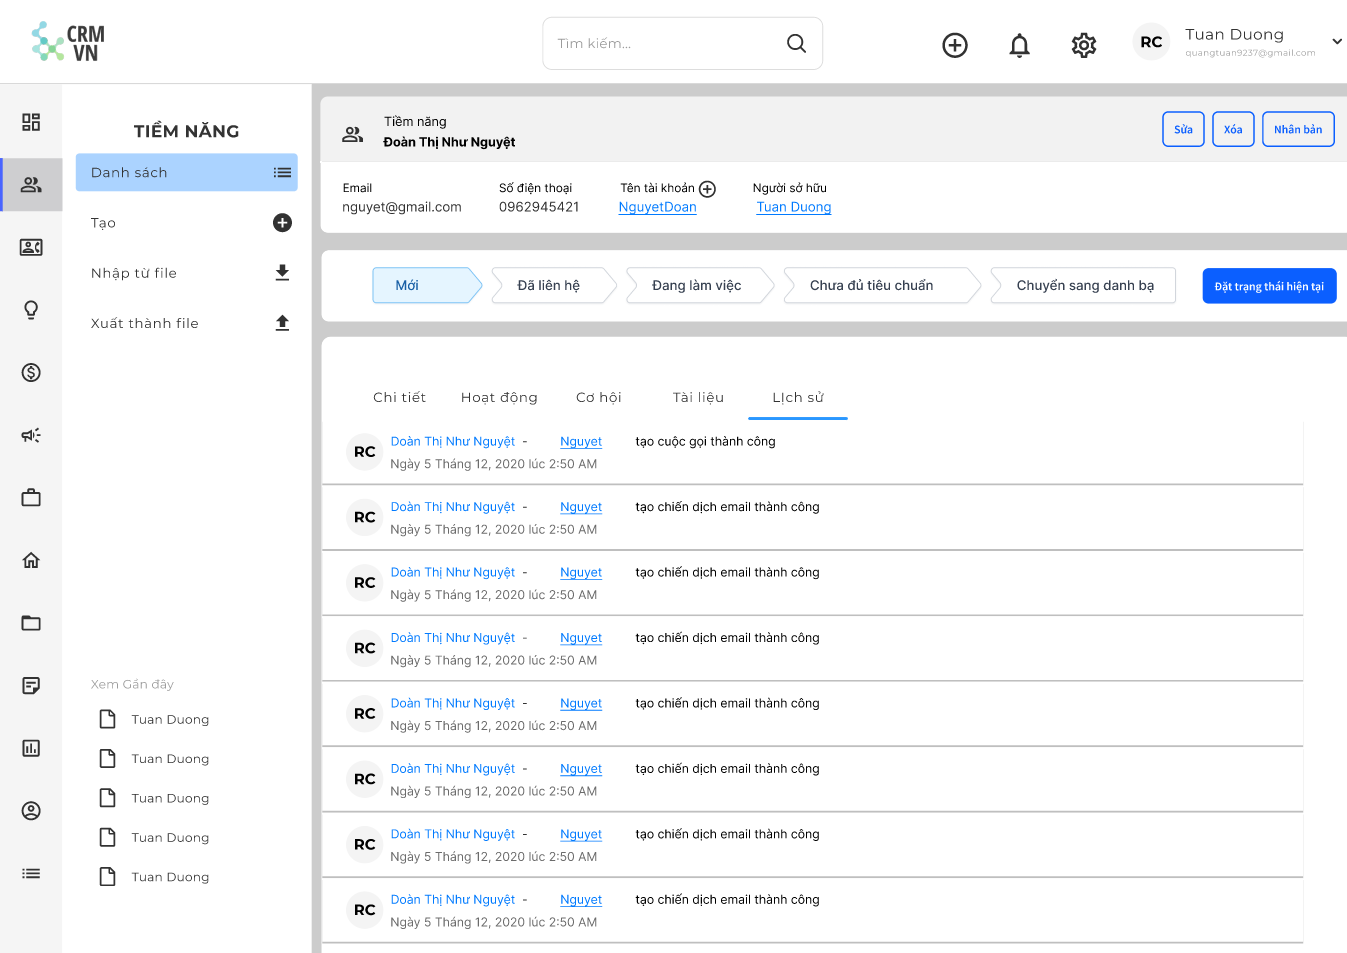
\includegraphics[width=\textwidth]{Img/Nguyet/lichsutiemnang.png}
                \vspace{0.5cm}
                \caption{Màn hình xem lịch sử thay đổi theo từng tiềm năng}
                \label{lichsuthaydoitiemnang}
            \end{figure}

            \item Nhập danh sách tiềm năng từ file \\
            Với tư cách người dùng, tôi muốn nhập danh sách tiềm năng từ file.

            \begin{figure}[H]
                \centering 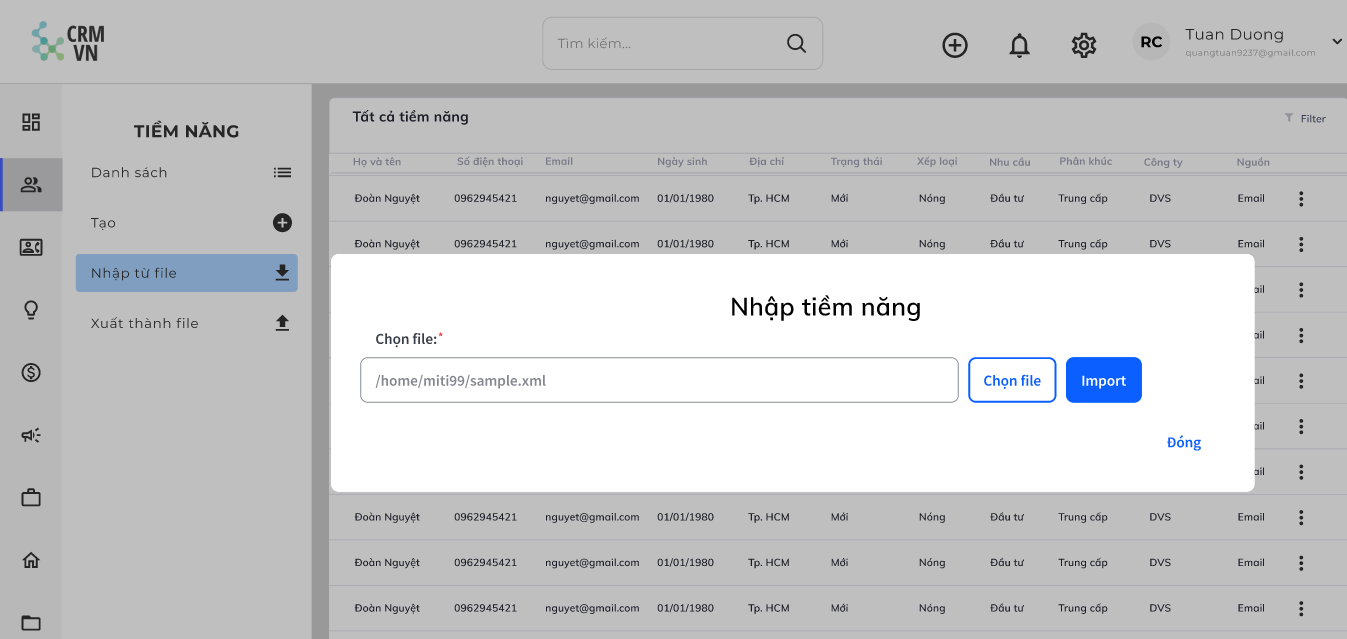
\includegraphics[width=\textwidth]{Img/Nguyet/importtiemnang.png}
                \vspace{0.5cm}
                \caption{Màn hình nhập danh sách tiềm năng từ file}
                \label{importtiemnang}
            \end{figure}

            \item Xuất danh sách tiềm năng thành file. \\
            Với tư cách người dùng, tôi muốn xuất danh sách tiềm năng thành file.

            \begin{figure}[H]
                \centering 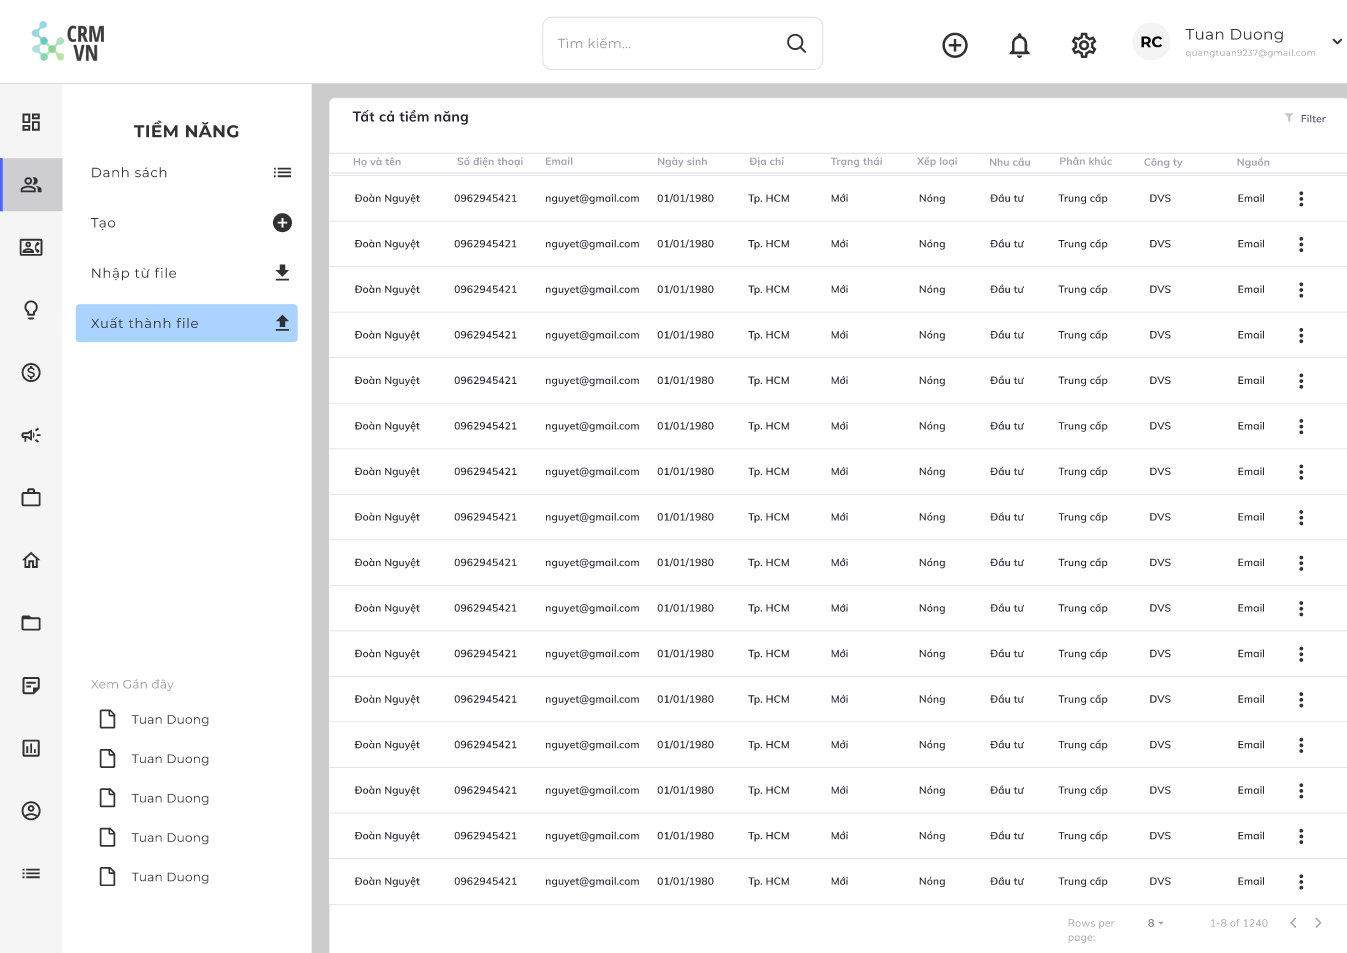
\includegraphics[width=\textwidth]{Img/Nguyet/exporttn.png}
                \vspace{0.5cm}
                \caption{Màn hình xuất danh sách tiềm năng thành file}
                \label{exporttiemnang}
            \end{figure}
        \end{itemize}

        \item Trang khách hàng
        \begin{itemize}
            \item Xem danh sách khách hàng \\
            Với tư cách người dùng, tôi muốn xem danh sách khách hàng.
            \begin{figure}[H]
                \centering 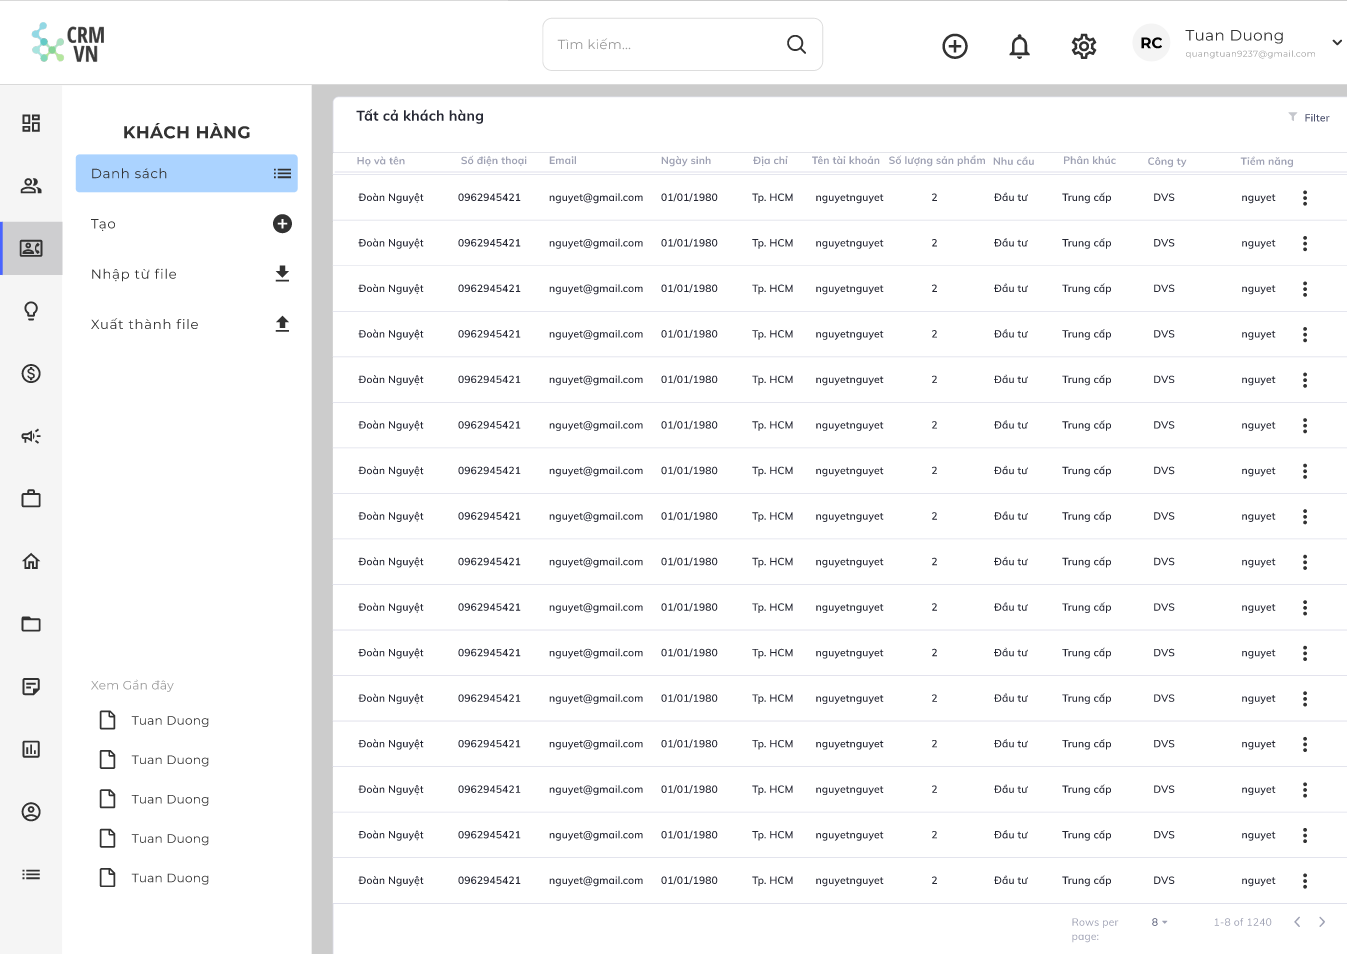
\includegraphics[width=\textwidth]{Img/Nguyet/Khachhang/danhsachkhachhang.png}
                \vspace{0.5cm}
                \caption{Màn hình xem danh sách khách hàng}
                \label{danhsachKH}
            \end{figure}

            \item Lọc thông tin khách hàng \\
            Với tư cách người dùng, tôi muốn lọc thông tin khách hàng.

            \begin{figure}[H]
                \centering 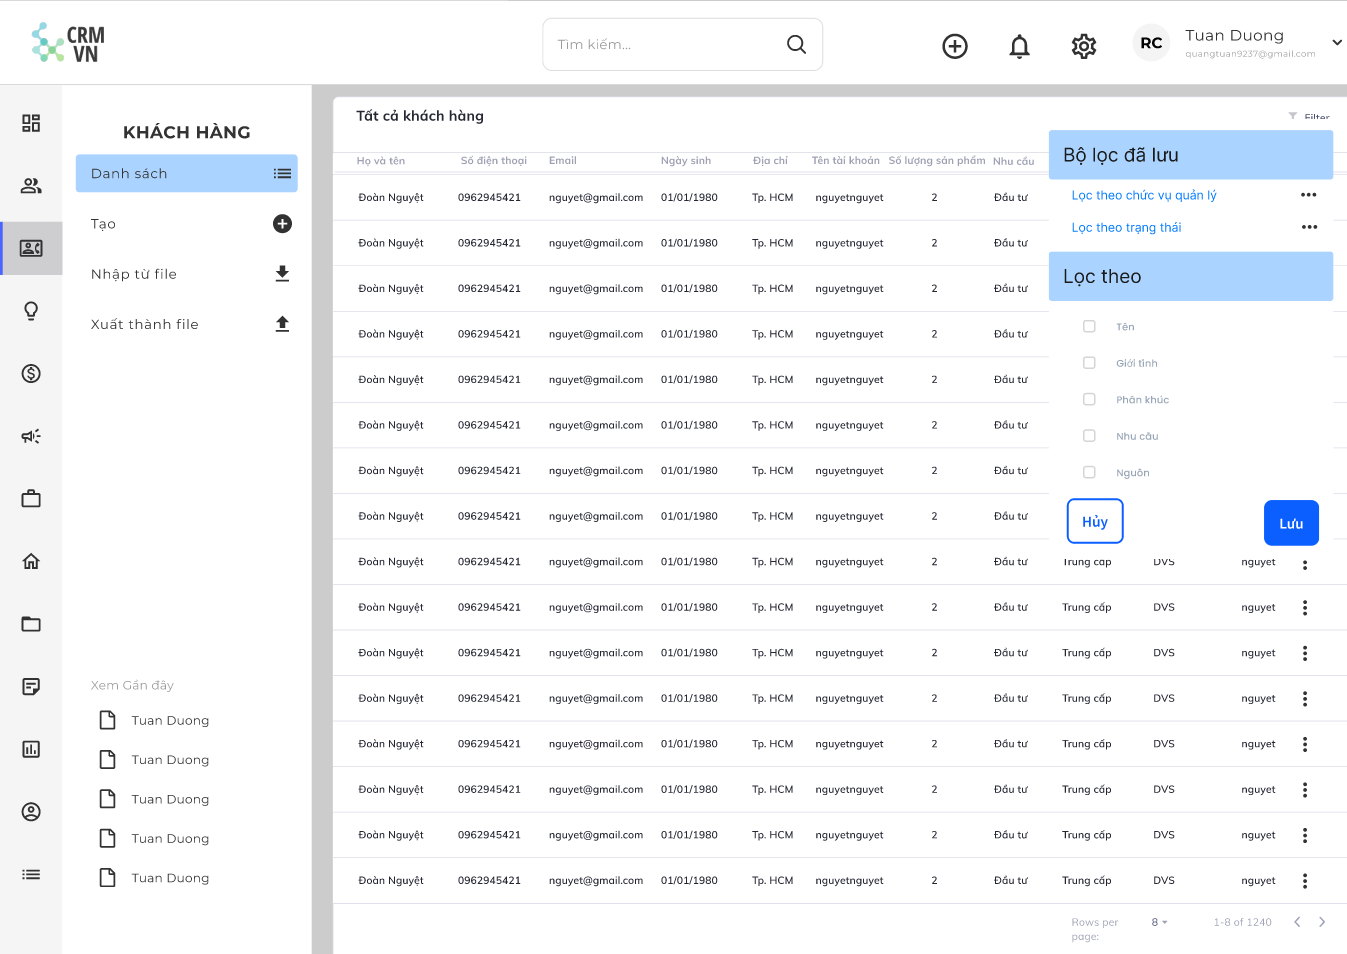
\includegraphics[width=\textwidth]{Img/Nguyet/Khachhang/lockhachhang.png}
                \vspace{0.5cm}
                \caption{Màn hình lọc thông tin khách hàng}
                \label{locKH}
            \end{figure}

            \item Tạo mới khách hàng \\
            Với tư cách người dùng, tôi muốn tạo mới khách hàng.
            \begin{figure}[H]
                \centering 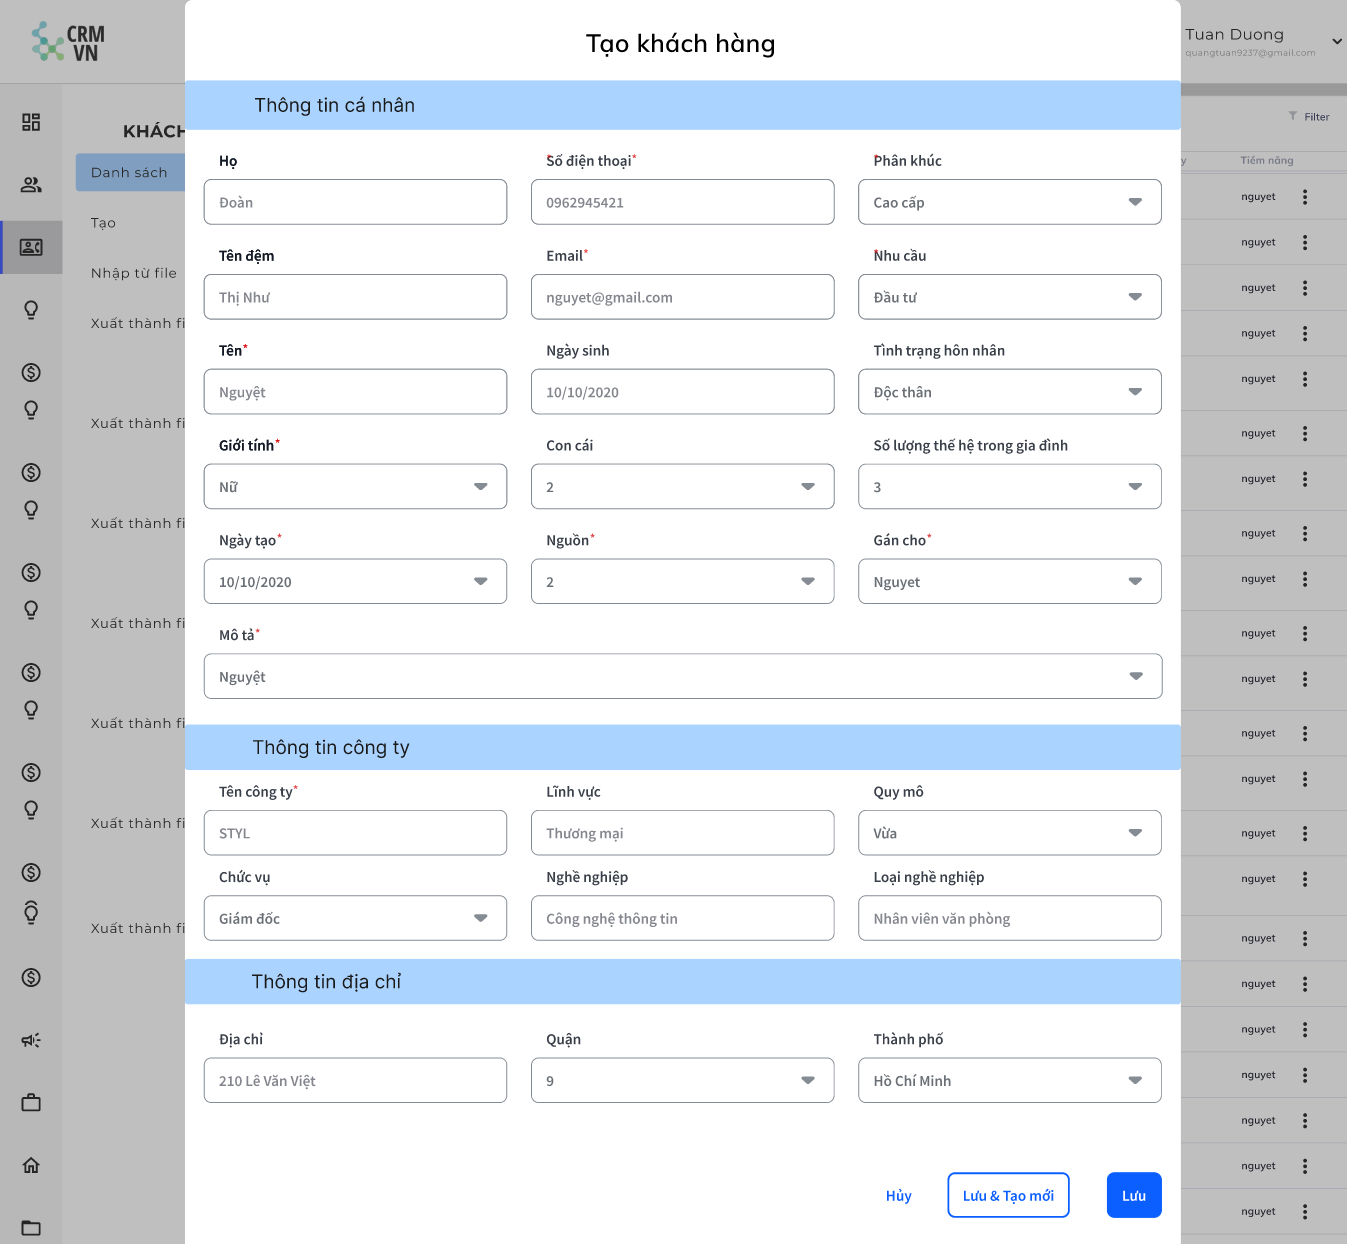
\includegraphics[width=\textwidth]{Img/Nguyet/Khachhang/themKH.png}
                \vspace{0.5cm}
                \caption{Màn hình tạo mới khách hàng}
                \label{taoKH}
            \end{figure}
            \item Xem chi tiết khách hàng \\
            Với tư cách người dùng, tôi muốn xem chi tiết khách hàng.
            \begin{figure}[H]
                \centering 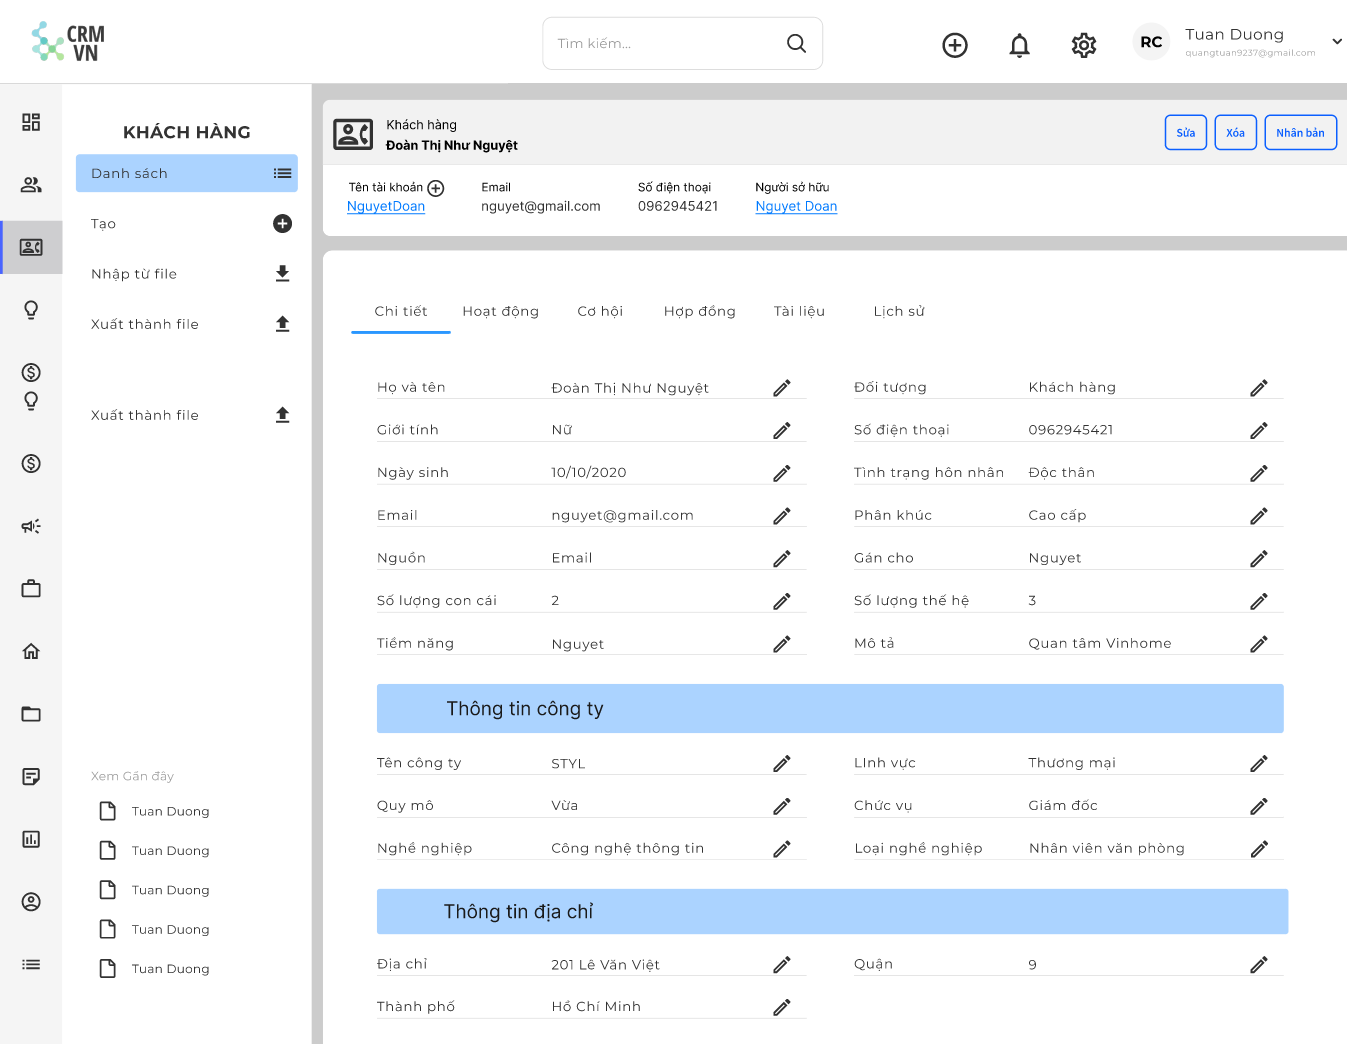
\includegraphics[width=\textwidth]{Img/Nguyet/Khachhang/chitietkhachhang.png}
                \vspace{0.5cm}
                \caption{Màn hình xem chi tiết khách hàng}
                \label{chitietKH}
            \end{figure}
            \item Sửa khách hàng \\
            Với tư cách người dùng, tôi muốn xem sửa khách hàng.
            \begin{figure}[H]
                \centering 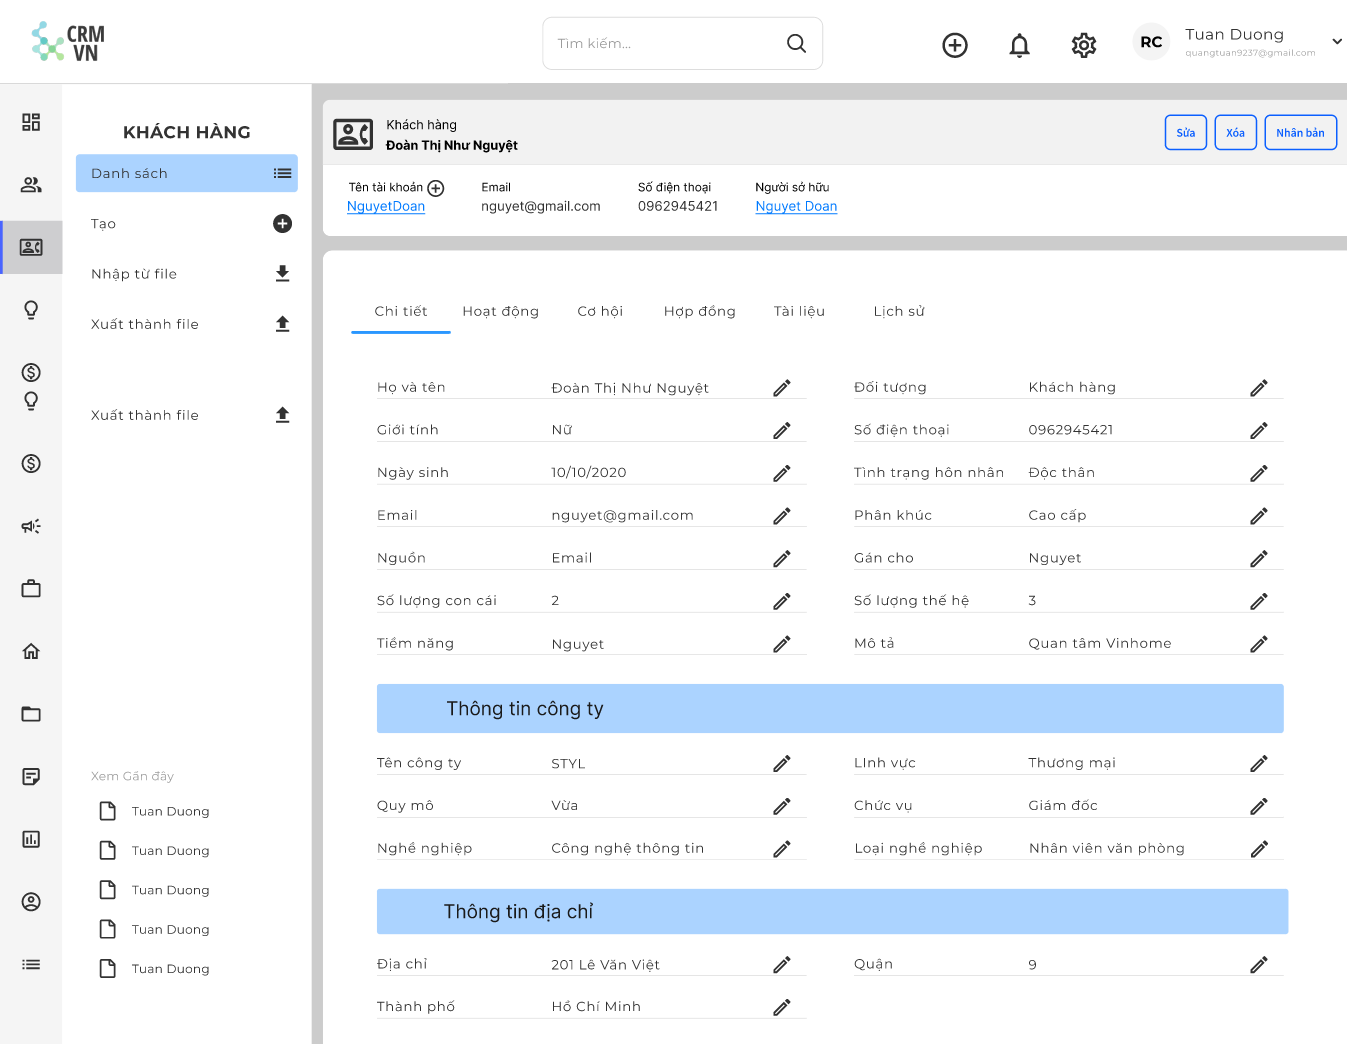
\includegraphics[width=\textwidth]{Img/Nguyet/Khachhang/chitietkhachhang.png}
                \vspace{0.5cm}
                \caption{Màn hình sửa thông tin khách hàng}
                \label{suaKH}
            \end{figure}
            \item Xóa khách hàng \\
            Với tư cách người dùng, tôi muốn xóa khách hàng.
            \begin{figure}[H]
                \centering 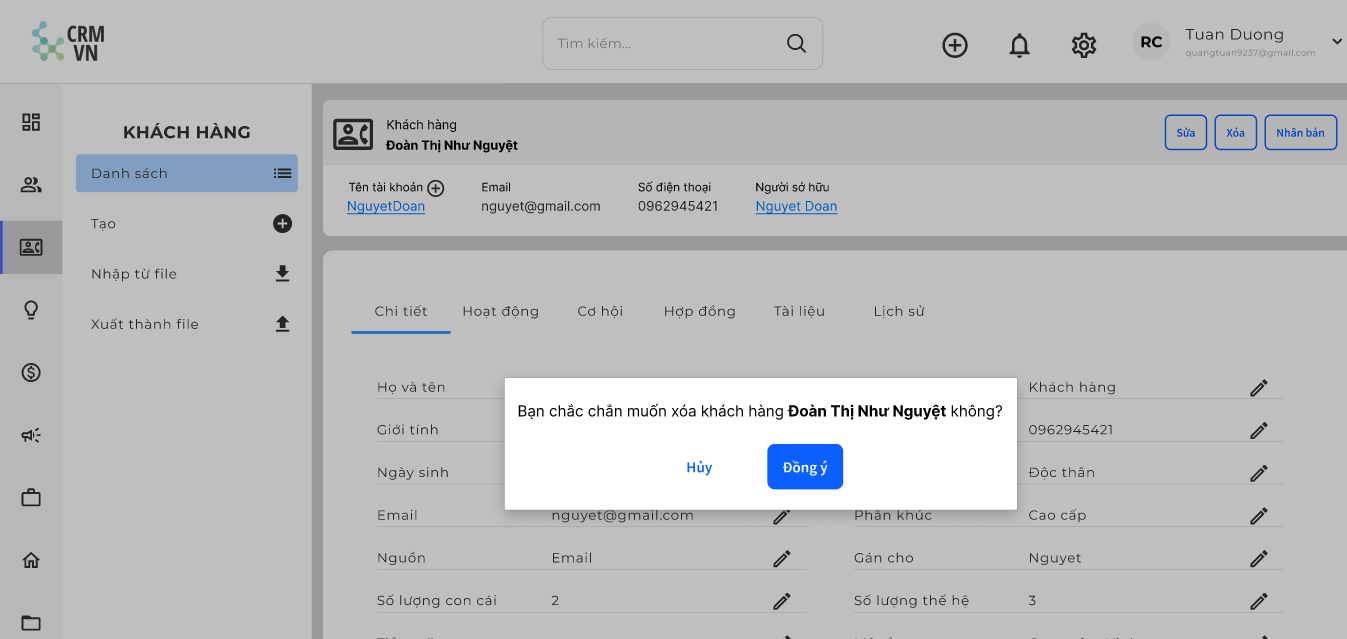
\includegraphics[width=\textwidth]{Img/Nguyet/Khachhang/xoakhachhang.png}
                \vspace{0.5cm}
                \caption{Màn hình xóa khách hàng}
                \label{xoaKH}
            \end{figure}
            \item Nhân bản khách hàng \\
            Với tư cách người dùng, tôi muốn nhân bản khách hàng.
            \begin{figure}[H]
                \centering 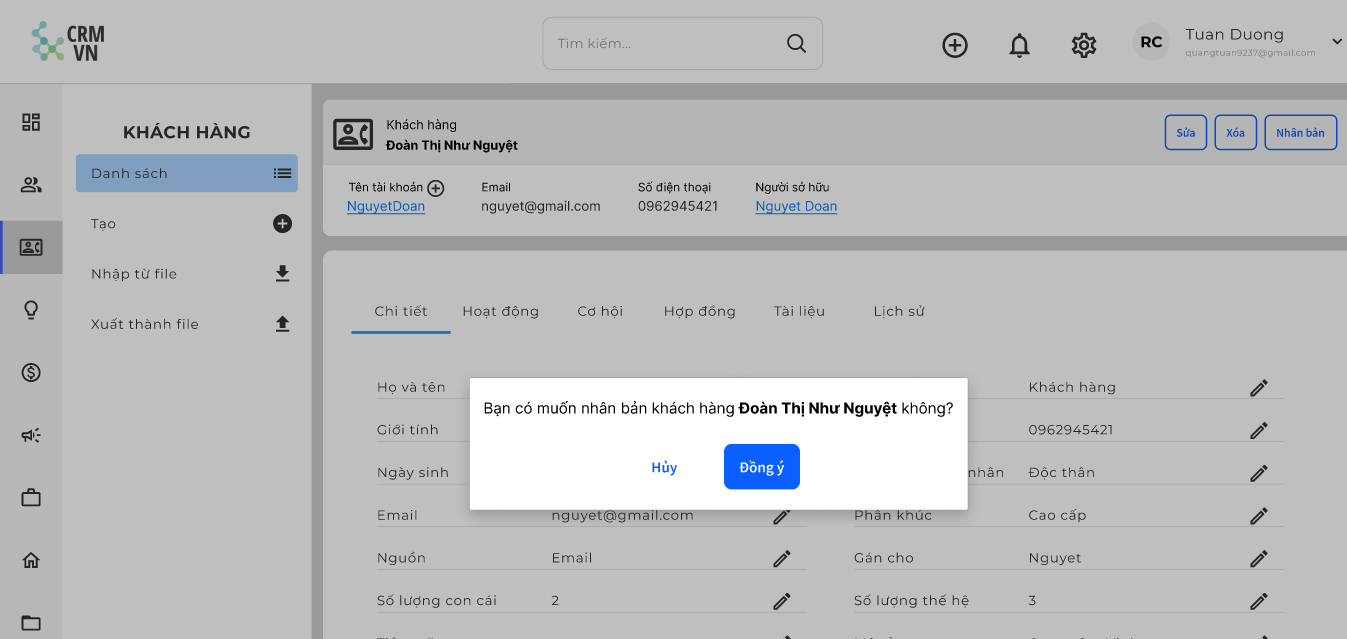
\includegraphics[width=\textwidth]{Img/Nguyet/Khachhang/nhanbankhachhang.png}
                \vspace{0.5cm}
                \caption{Màn hình nhân bản khách hàng}
                \label{nhanbanKH}
            \end{figure}
            \item Tạo tài khoản cho khách hàng \\

            \begin{figure}[H]
                \centering 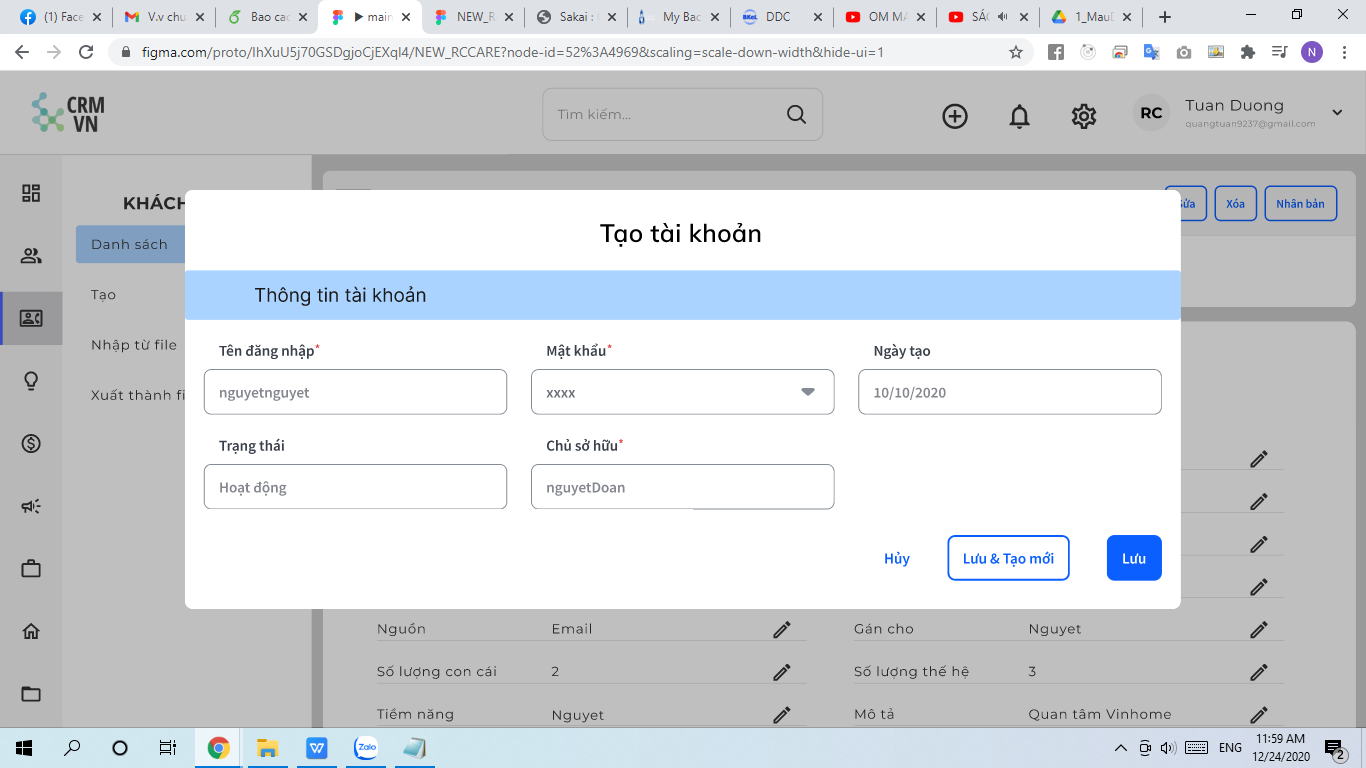
\includegraphics[width=\textwidth]{Img/Nguyet/Khachhang/taoTKKH.png}
                \vspace{0.5cm}
                \caption{Màn hình tạo tài khoản khách hàng}
                \label{taoTKKH}
            \end{figure}

            \item Tạo hoạt động khác cho khách hàng \\
            Với tư cách người dùng, tôi muốn tạo các hoạt động: cuộc gọi, SMS, email, ... cho khách hàng.

            \begin{figure}[H]
                \centering 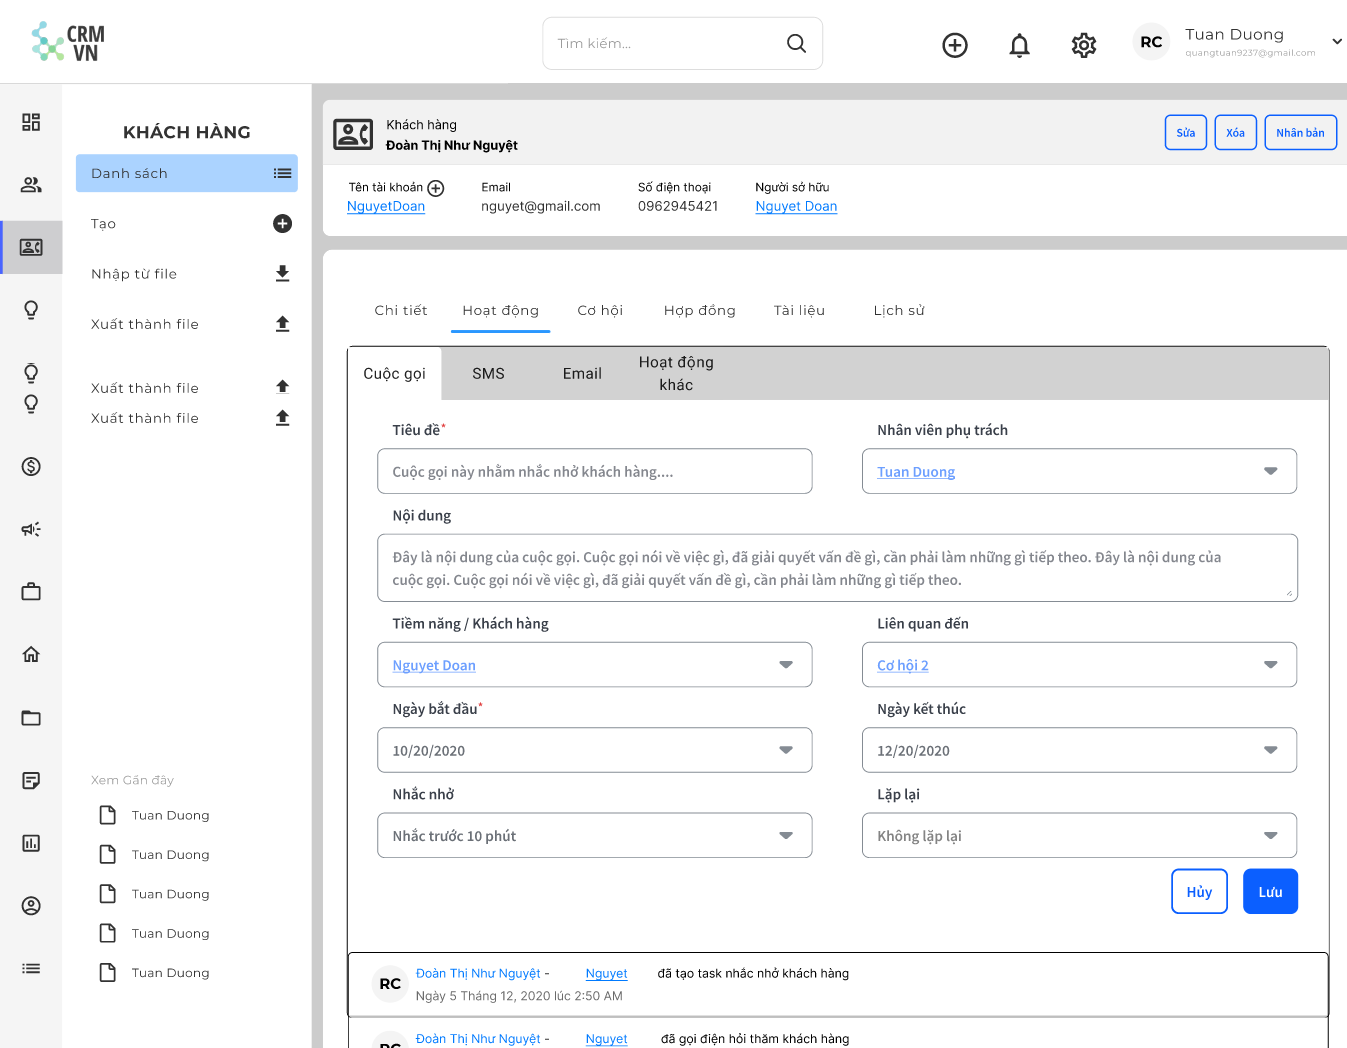
\includegraphics[width=\textwidth]{Img/Nguyet/Khachhang/cuocgoiKH.png}
                \vspace{0.5cm}
                \caption{Màn hình cuộc gọi cho khách hàng}
                \label{taocuocgoiKH}
            \end{figure}

            \begin{figure}[H]
                \centering 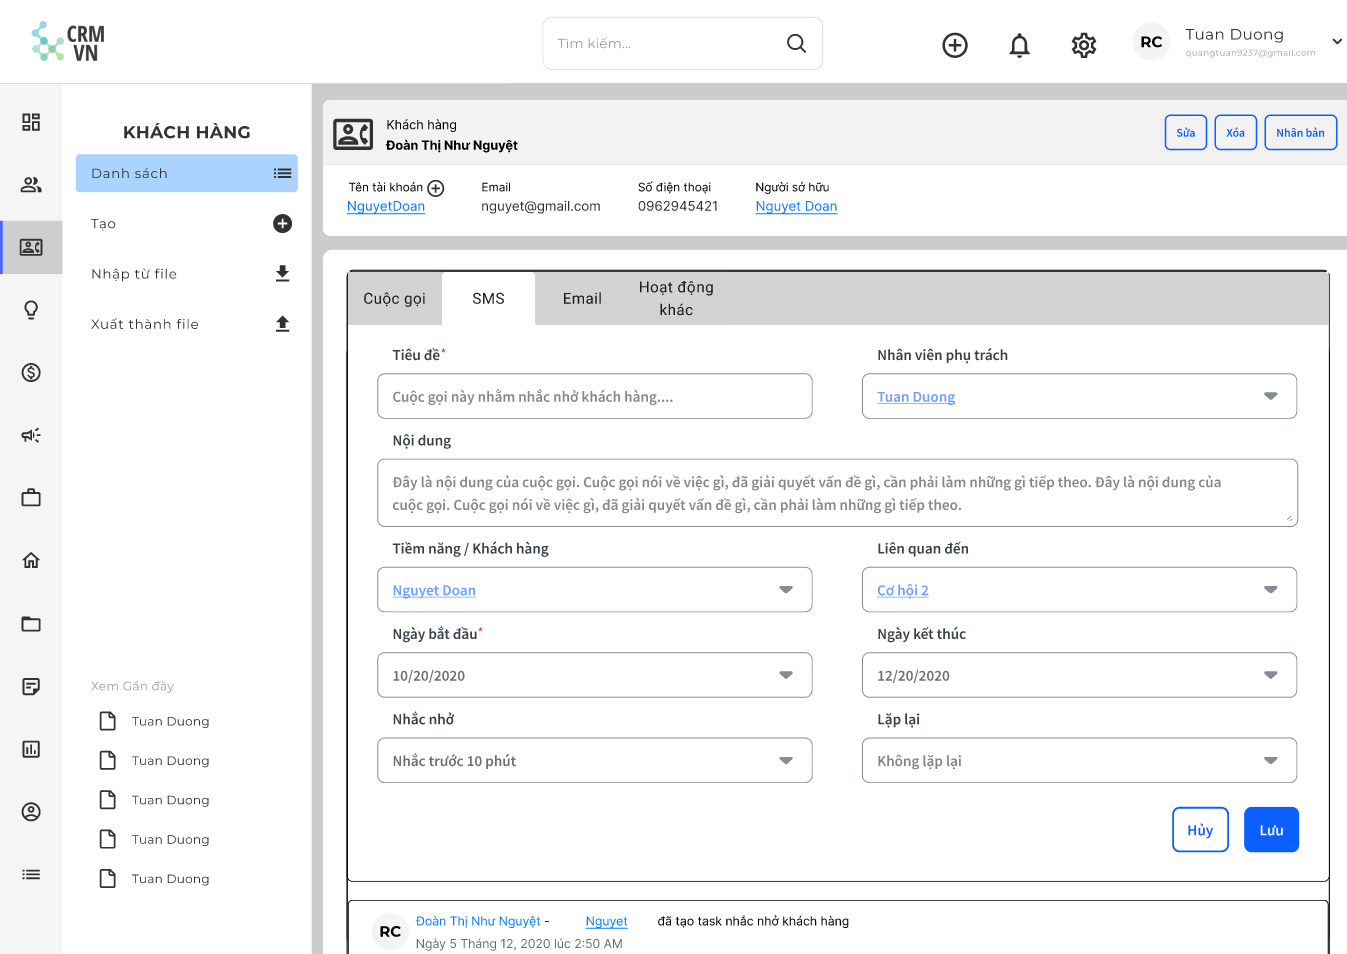
\includegraphics[width=\textwidth]{Img/Nguyet/Khachhang/SMSKH.png}
                \vspace{0.5cm}
                \caption{Màn hình gửi SMS khách hàng}
                \label{guiSMSKH}
            \end{figure}

            \begin{figure}[H]
                \centering 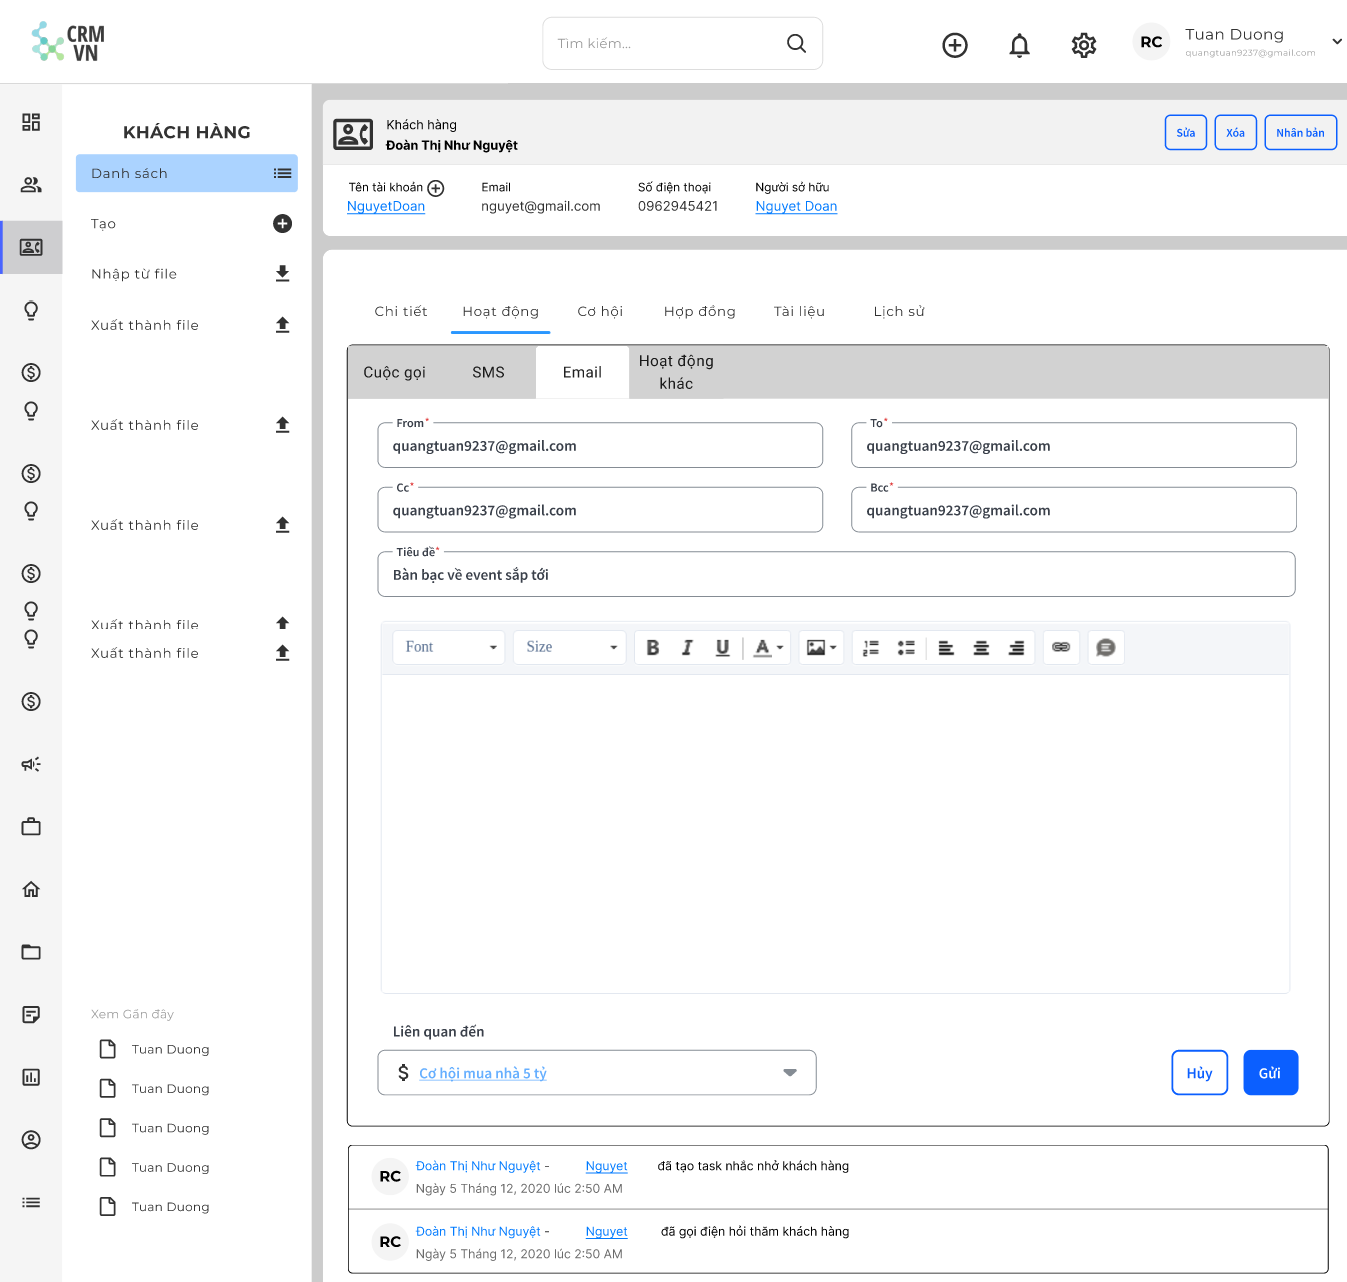
\includegraphics[width=\textwidth]{Img/Nguyet/Khachhang/emailKH.png}
                \vspace{0.5cm}
                \caption{Màn hình tạo email gửi khách hàng}
                \label{guiemailKH}
            \end{figure}

            \begin{figure}[H]
                \centering 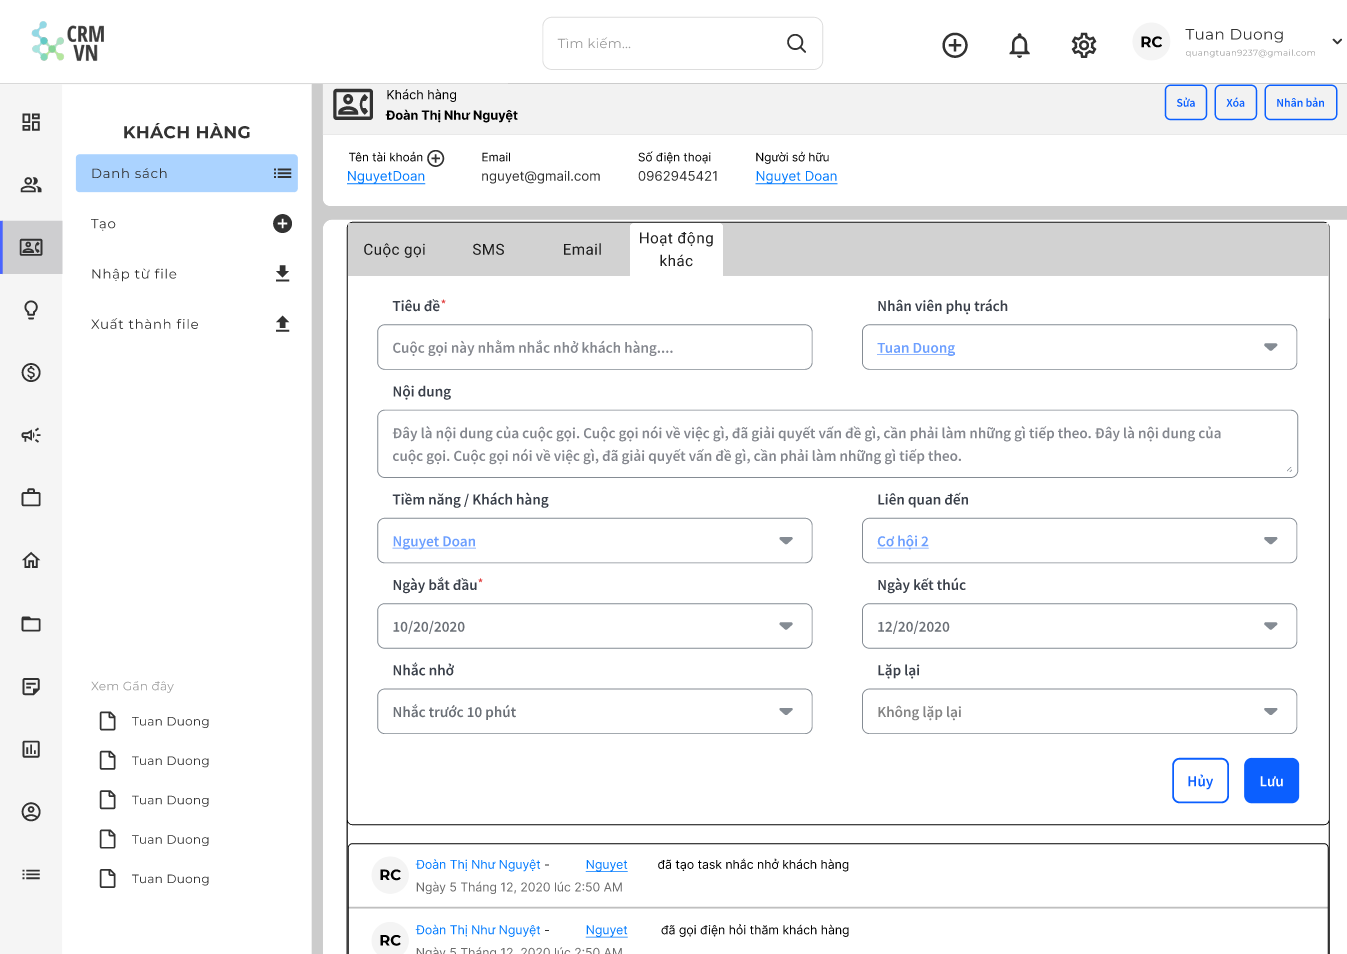
\includegraphics[width=\textwidth]{Img/Nguyet/Khachhang/HoatdongkhacKH.png}
                \vspace{0.5cm}
                \caption{Màn hình tạo hoạt động khác cho khách hàng}
                \label{taohoadongkhacKH}
            \end{figure}

            \item Xem danh sách các hoạt động đã thực hiện cho từng khách hàng
            \\ Với tư cách người dùng, tôi muốn xem danh sách các hoạt động đã tạo cho khách hàng.

            \begin{figure}[H]
                \centering 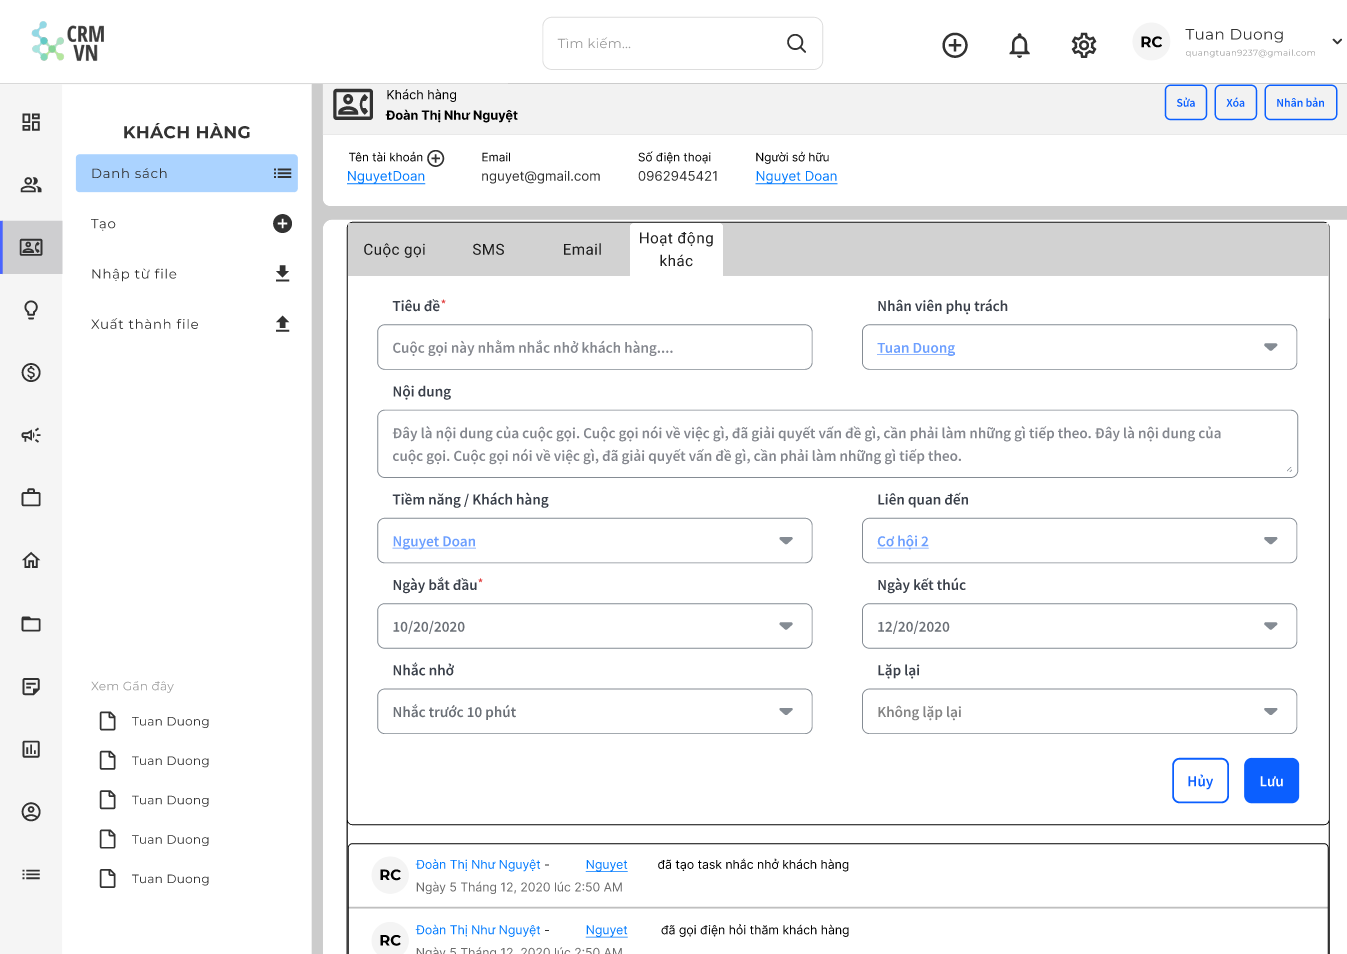
\includegraphics[width=\textwidth]{Img/Nguyet/Khachhang/HoatdongkhacKH.png}
                \vspace{0.5cm}
                \caption{Màn hình danh sách hoạt động khách hàng}
                \label{dshoatdongKH}
            \end{figure}

            \item Tạo cơ hội cho khách hàng \\
            Với tư cách khách hàng, tôi muốn tạo cơ hội cho khách hàng để thực hiện các chiến lược chăm sóc khách hàng tốt hơn.
            \begin{figure}[H]
                \centering 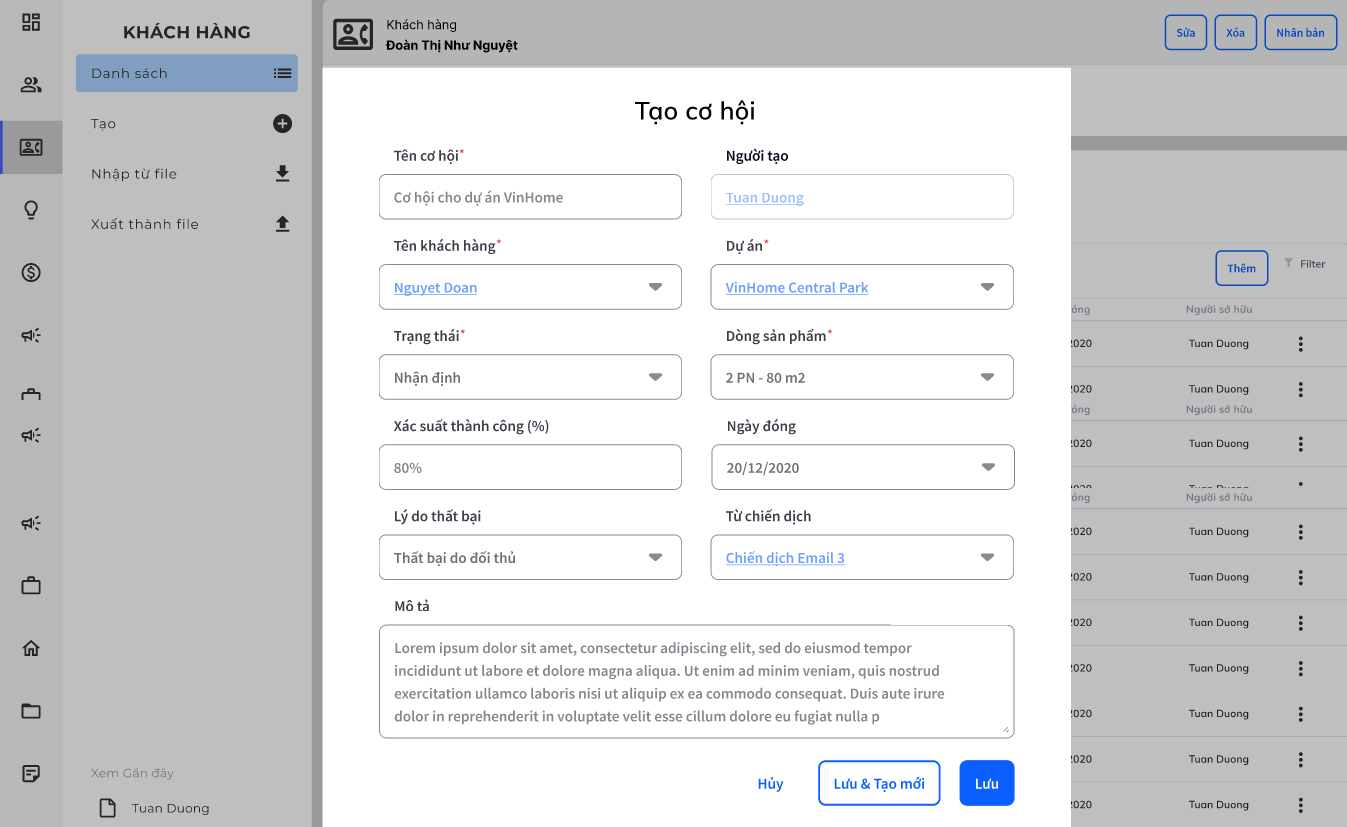
\includegraphics[width=\textwidth]{Img/Nguyet/Khachhang/themCohoiKH.png}
                \vspace{0.5cm}
                \caption{Màn hình tạo cơ hội cho khách hàng}
                \label{themcohoiKH}
            \end{figure}

            \item Xem danh sách cơ hội theo khách hàng \\
            Với tư cách khách hàng, tôi muốn xem danh sách cơ hội theo khách hàng.

            \begin{figure}[H]
                \centering 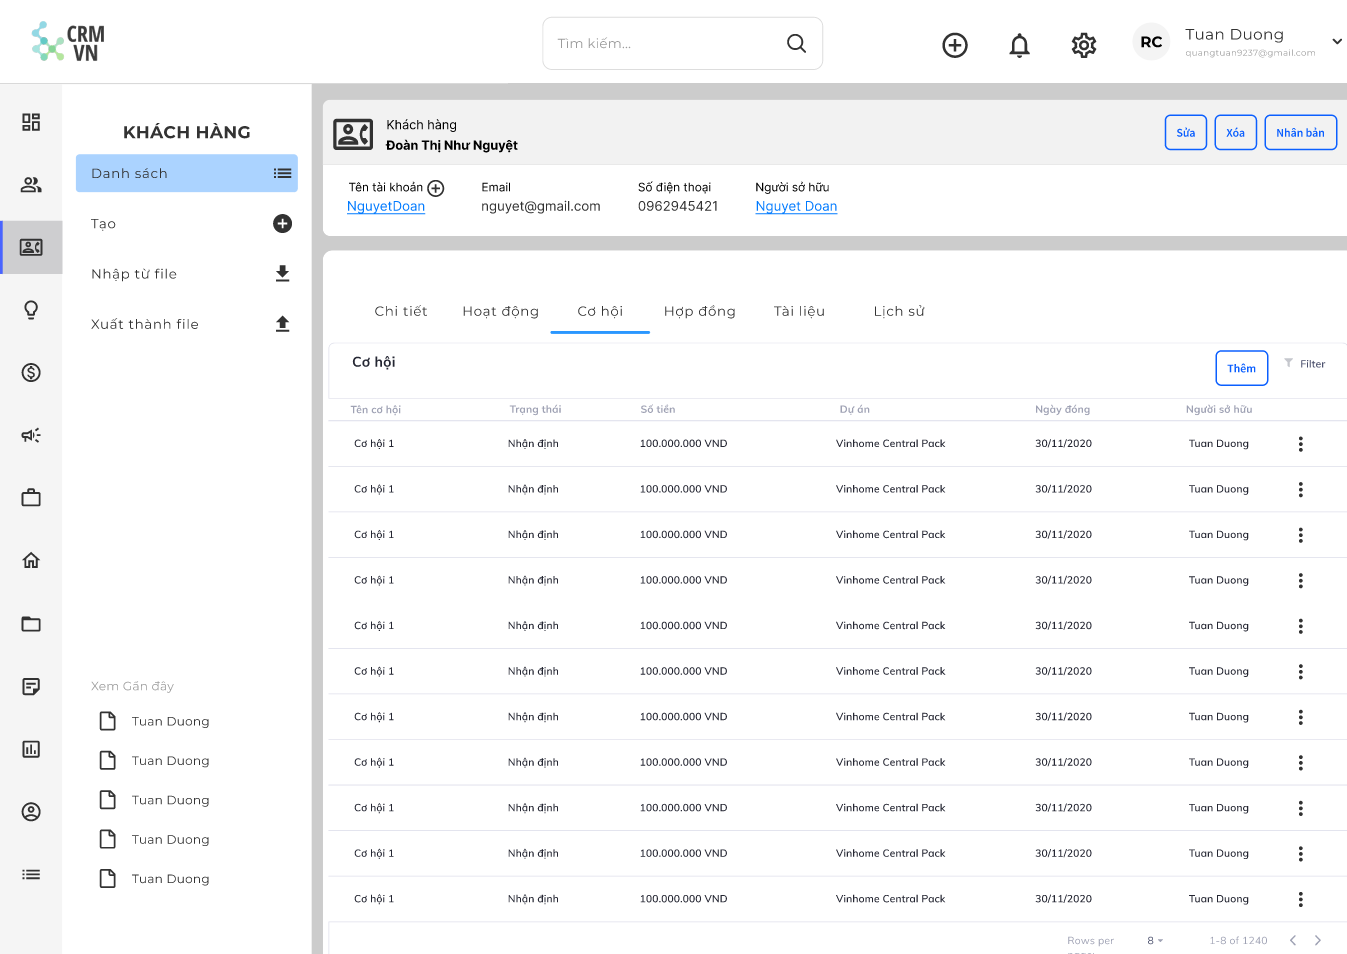
\includegraphics[width=\textwidth]{Img/Nguyet/Khachhang/xemdanhsachcohoi.png}
                \vspace{0.5cm}
                \caption{Màn hình danh sách cơ hội khách hàng}
                \label{dscohoiKH}
            \end{figure}


            \item Xem chi tiết từng cơ hội theo khách hàng \\
            Với tư cách người dùng, tôi muốn xem chi tiết từng cơ hội theo khách hàng.
            \begin{figure}[H]
                \centering 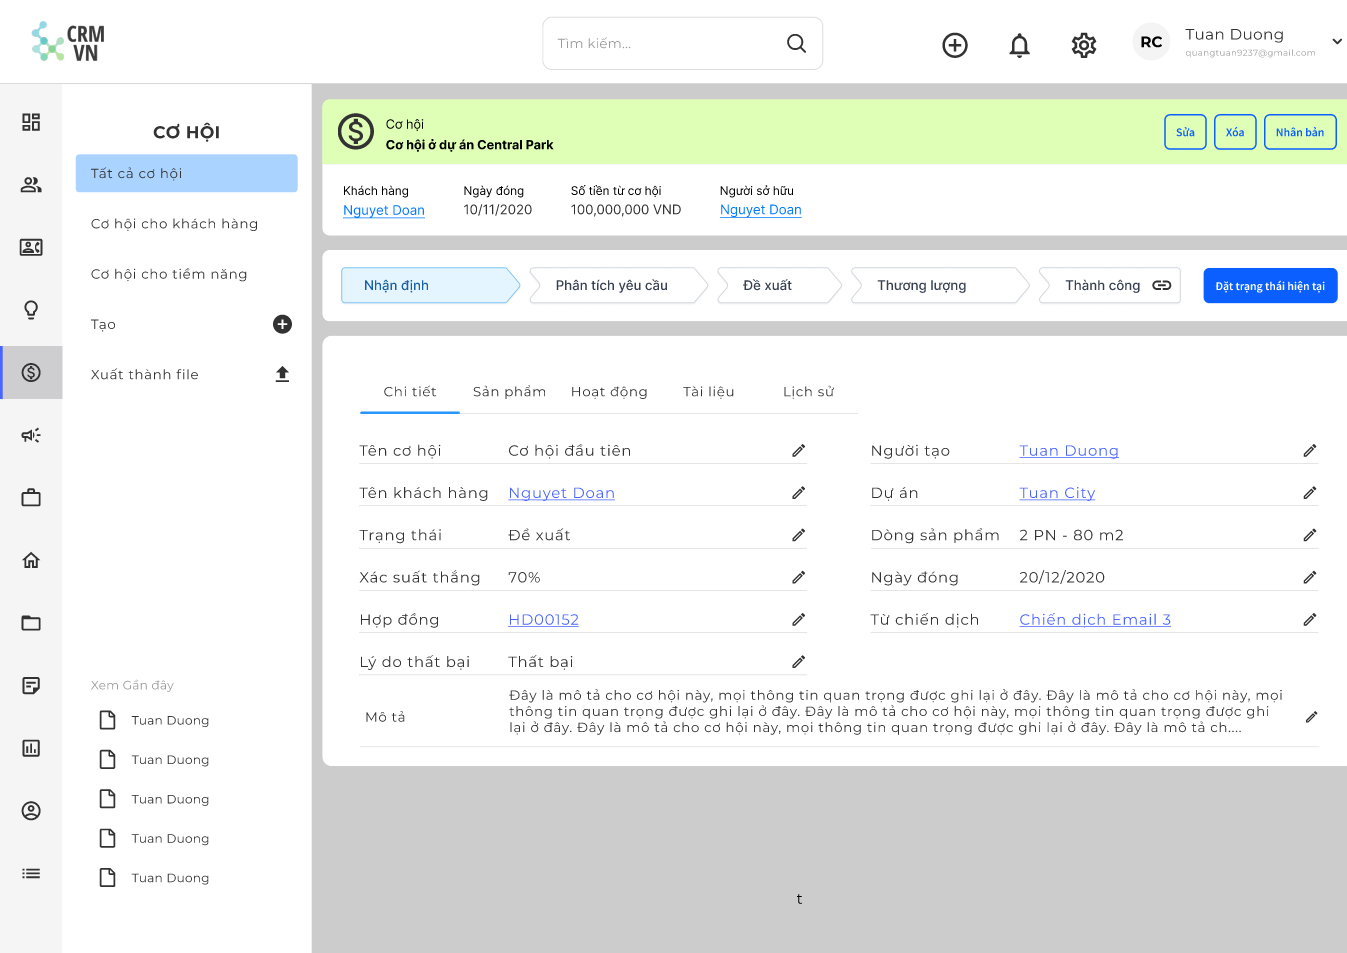
\includegraphics[width=\textwidth]{Img/Nguyet/chitietcohoi.png}
                \vspace{0.5cm}
                \caption{Màn hình chi tiết cơ hội của khách hàng}
                \label{chitietcohoiKH}
            \end{figure}
            \item Xem danh sách tài liệu theo từng khách hàng
            \\ Với tư cách người dùng, tôi muốn xem danh sách tài liệu theo từng khách hàng.
            \begin{figure}[H]
                \centering 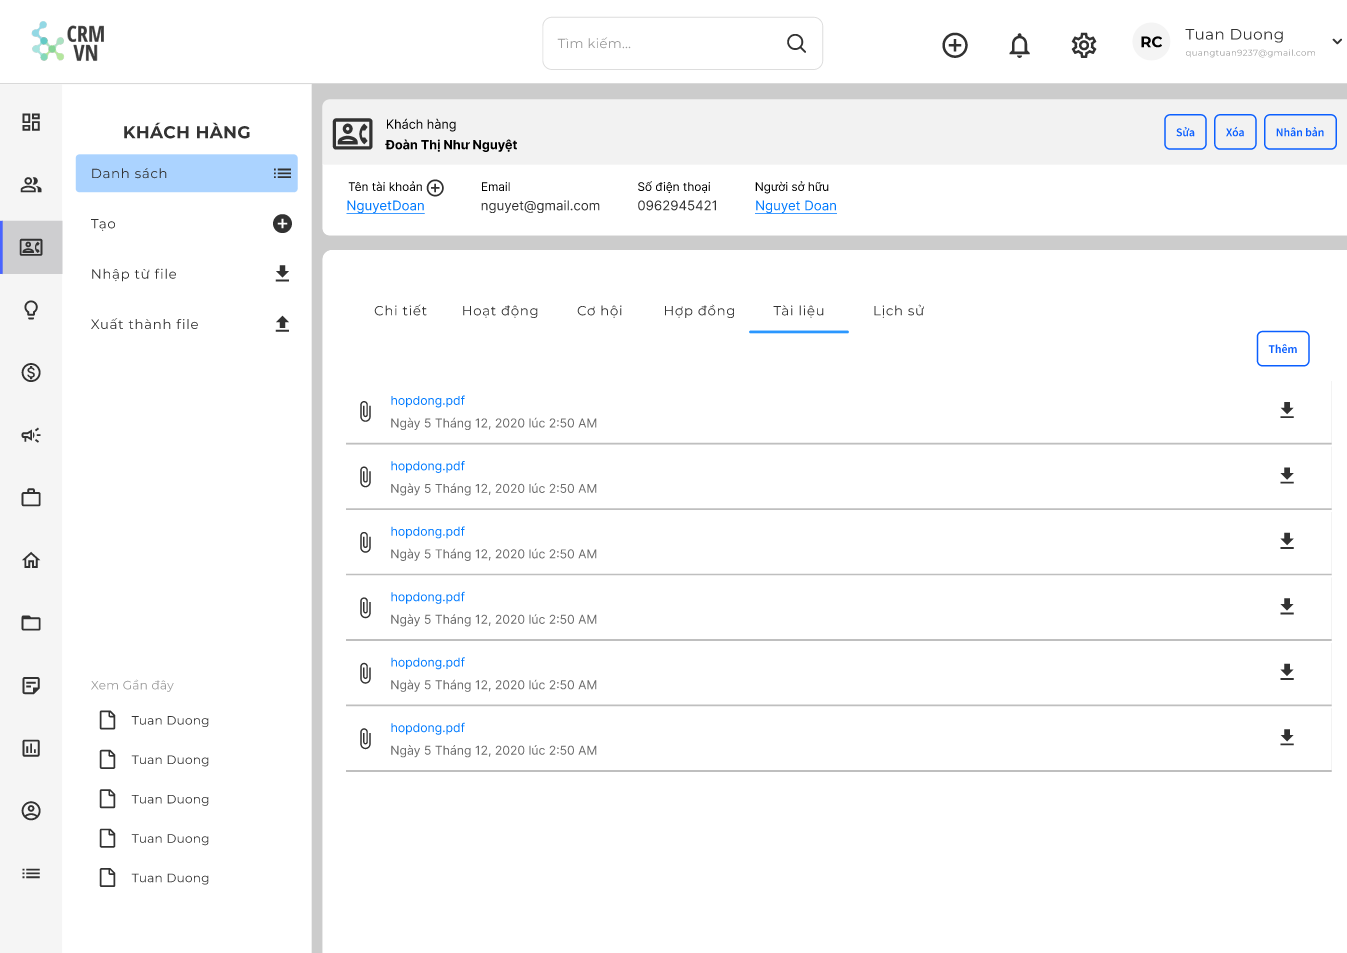
\includegraphics[width=\textwidth]{Img/Nguyet/Khachhang/dsTailieu.png}
                \vspace{0.5cm}
                \caption{Màn hình danh sách tài liệu khách hàng}
                \label{dstailieuKH}
            \end{figure}
            \item Thêm tài liệu cho khách hàng \\
            Với tư cách người dùng, tôi muốn thêm tài liệu cho khách hàng.
            \begin{figure}[H]
                \centering 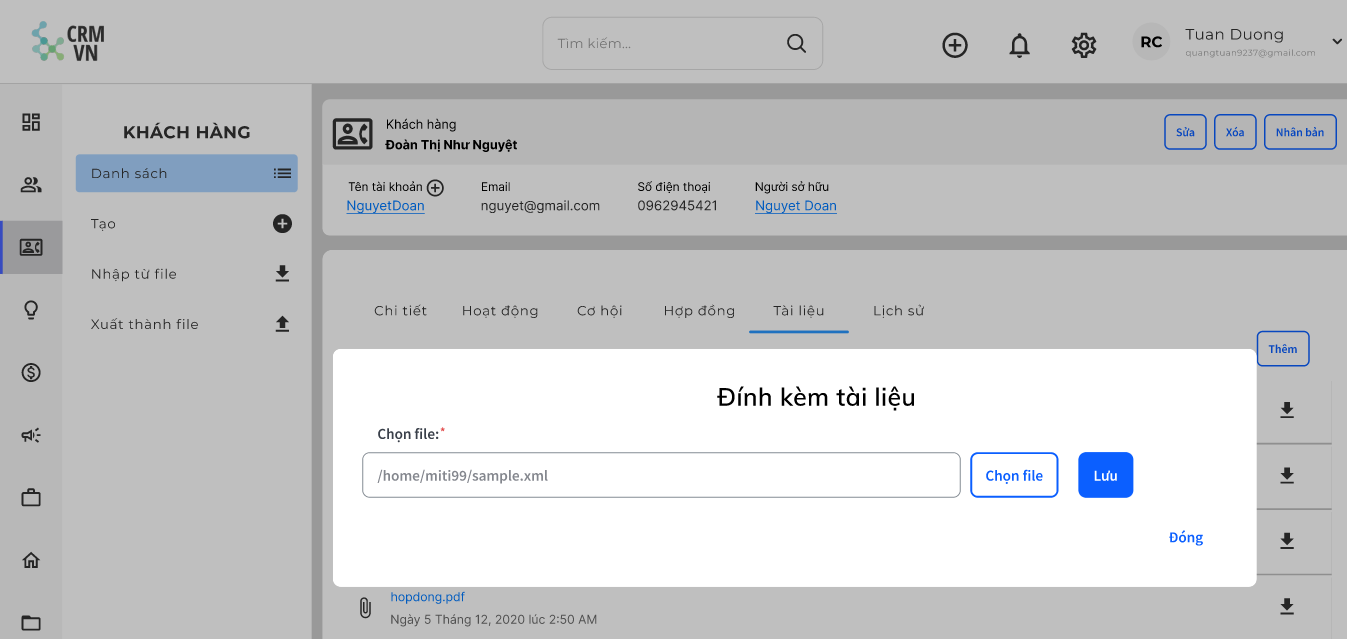
\includegraphics[width=\textwidth]{Img/Nguyet/Khachhang/Themtailieu.png}
                \vspace{0.5cm}
                \caption{Màn hình thêm tài liệu khách hàng}
                \label{themtailieuKH}
            \end{figure}
            \item Sửa tài liệu cho khách hàng \\
            Với tư cách người dùng, tôi muốn sửa tài liệu thuộc khách hàng.
            \item Xóa tài liệu cho khách hàng
            \\Với tư cách người dùng, tôi muốn xóa tài liệu thuộc khách hàng.

            \item Tải tài liệu theo từng khách hàng
            \\Với tư cách người dùng, tôi muốn tải tài liệu theo từng khách hàng.

            \item Xem lịch sử thay đổi theo từng khách hàng
            \\Với tư cách từ người dùng, tôi muốn xem lịch sử thay đổi theo từng khách hàng.
            \begin{figure}[H]
                \centering 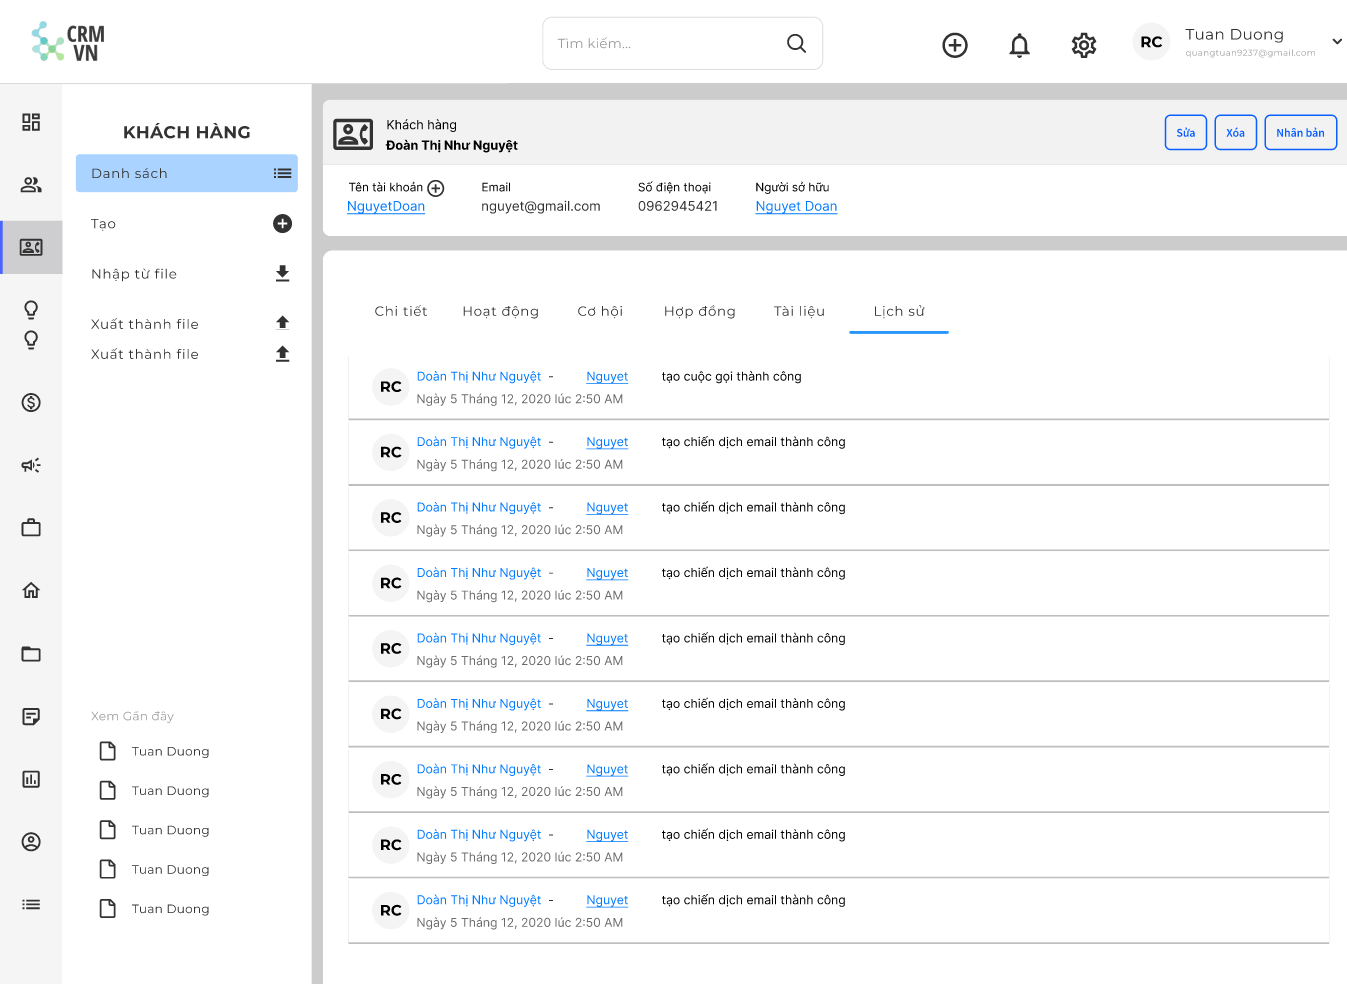
\includegraphics[width=\textwidth]{Img/Nguyet/Khachhang/lichsuKH.png}
                \vspace{0.5cm}
                \caption{Màn hình xem lịch sử thay đổi khách hàng}
                \label{lichsuKH}
            \end{figure}
            \item Nhập danh sách khách hàng từ file
            \\Với tư cách người dùng, tôi muốn nhập danh sách khách hàng từ file.
            \begin{figure}[H]
                \centering \includegraphics[width=\textwidth]{Img/Nguyet/Khachhang/importKH.png}
                \vspace{0.5cm}
                \caption{Màn hình nhập danh sách từ file khách hàng}
                \label{importKH}
            \end{figure}
            \item Xuất danh sách khách hàng từ file
            \\Với tư cách người dùng, tôi muốn xuất danh sách khách hàng thành file.
            \begin{figure}[H]
                \centering \includegraphics[width=\textwidth]{Img/Nguyet/Khachhang/exportKH.png}
                \vspace{0.5cm}
                \caption{Màn hình xuất danh sách khách hàng thành file}
                \label{exportKH}
            \end{figure}
            \item Xem danh sách hợp đồng theo từng khách hàng
            \\Với tư cách người dùng, tôi muốn xem danh sách hợp đồng theo từng khách hàng.
            \begin{figure}[H]
                \centering \includegraphics[width=\textwidth]{Img/Nguyet/Khachhang/danhsachhopdongKH.png}
                \vspace{0.5cm}
                \caption{Màn hình xem danh sách hợp đồng của khách hàng}
                \label{dshopdongKH}
            \end{figure}
            \item Xem chi tiết hợp đồng theo từng khách hàng
            \\Với tư cách người dùng, tôi muốn xem chi tiết hợp đồng theo từng khách hàng.
            \begin{figure}[H]
                \centering \includegraphics[width=\textwidth]{Img/Nguyet/Khachhang/chitiethopdongKH.png}
                \vspace{0.5cm}
                \caption{Màn hình chi tiết hợp đồng khách hàng}
                \label{chitietHDKH}
            \end{figure}
            \item Thêm hợp đồng theo từng khách hàng \\
            Với tư cách người dùng, tôi muốn thêm hợp đồng theo từng khách hàng.

            \begin{figure}[H]
                \centering \includegraphics[width=\textwidth]{Img/Nguyet/Khachhang/taohopdongKH.png}
                \vspace{0.5cm}
                \caption{Màn hình thêm hợp đồng cho khách hàng}
                \label{themHDKH}
            \end{figure}
        \end{itemize}

        \item Trang đề xuất cơ hội
        \begin{itemize}
            \item Xem danh đề xuất cơ hội cho khách hàng \\
            Với tư cách người dùng, tôi muốn xem danh sách đề xuất cơ hội cho khách hàng.
            \begin{figure}[H]
                \centering \includegraphics[width=\textwidth]{Img/Nguyet/DexuatCohoi/danhsachdexuat.png}
                \vspace{0.5cm}
                \caption{Màn hình xem đề xuất cơ hộ cho khách hàng}
                \label{dexuatcohoiKH}
            \end{figure}
            \item Xem danh đề xuất cơ hội cho tiềm năng\\
            Với tư cách người dùng, tôi muốn xem danh sách đề xuất cơ hội cho tiềm năng.
            \begin{figure}[H]
                \centering \includegraphics[width=\textwidth]{Img/Nguyet/DexuatCohoi/dsdexuattiemnang.png}
                \vspace{0.5cm}
                \caption{Màn hình xem đề xuất cơ hội cho tiềm năng}
                \label{dexuatcohoiTN}
            \end{figure}
            \item Xem danh đề xuất cơ hội cho dòng sản phẩm \\
            Với tư cách người dùng, tôi muốn xem danh sách đề xuất cơ hội cho dòng sản phẩm.
            \begin{figure}[H]
                \centering \includegraphics[width=\textwidth]{Img/Nguyet/DexuatCohoi/dsdexuatdongsp.png}
                \vspace{0.5cm}
                \caption{Màn hình xem đề xuất cơ hội cho dòng sản phẩm}
                \label{dexuatcohoiDSP}
            \end{figure}
            \item Tạo cơ hội từ đề xuất\\
            Với tư cách người dùng, tôi muốn tạo cơ hội từ đề xuất.
            \begin{figure}[H]
                \centering \includegraphics[width=\textwidth]{Img/Nguyet/DexuatCohoi/taocohodexuat.png}
                \vspace{0.5cm}
                \caption{Màn hình tạo cơ hội từ đề xuất}
                \label{taocohoitudx}
            \end{figure}
        \end{itemize}
        \item Trang cơ hội
        \begin{itemize}
            \item Xem danh sách cơ hội
            \\Với tư cách người dùng, tôi muốn xem danh sách cơ hội.
            \begin{figure}[H]
                \centering \includegraphics[width=\textwidth]{Img/Nguyet/Cohoi/dscohoi.png}
                \vspace{0.5cm}
                \caption{Màn hình xem danh sách cơ hội }
                \label{dscohoi}
            \end{figure}
            \item Lọc thông tin cơ hội
            \\Với tư cách người dùng, tôi muốn lọc thông tin cơ hội.
            \begin{figure}[H]
                \centering \includegraphics[width=\textwidth]{Img/Nguyet/Cohoi/loccohoi.png}
                \vspace{0.5cm}
                \caption{Màn hình lọc thông tin cơ hội }
                \label{loccohoi}
            \end{figure}
            \item Tạo mới cơ hội \\
            Với tư cách người dùng, tôi muốn tạo mới cơ hội.
            \begin{figure}[H]
                \centering \includegraphics[width=\textwidth]{Img/Nguyet/Cohoi/taocohoi.png}
                \vspace{0.5cm}
                \caption{Màn hình tạo cơ hội }
                \label{taocohoii}
            \end{figure}
            \item Xem chi tiết cơ hội \\
            Với tư cách người dùng, tôi muốn xem chi tiết cơ hội.
            \begin{figure}[H]
                \centering \includegraphics[width=\textwidth]{Img/Nguyet/Cohoi/chitietcohoi.png}
                \vspace{0.5cm}
                \caption{Màn hình xem chi tiết cơ hội }
                \label{chitietcohoii}
            \end{figure}
            \item Sửa cơ hội \\
            Với tư cách người dùng, tôi muốn sửa cơ hội.
            \begin{figure}[H]
                \centering \includegraphics[width=\textwidth]{Img/Nguyet/Cohoi/chitietcohoi.png}
                \vspace{0.5cm}
                \caption{Màn hình sửa cơ hội }
                \label{suacohoii}
            \end{figure}
            \item Xóa cơ hội \\
            Với tư cách người dùng, tôi muốn xóa cơ hội.
            \begin{figure}[H]
                \centering \includegraphics[width=\textwidth]{Img/Nguyet/Cohoi/xoacohoi.png}
                \vspace{0.5cm}
                \caption{Màn hình xóa cơ hội }
                \label{xoacohoi}
            \end{figure}
            \item Nhân bản cơ hội \\
            Với tư cách người dùng, tôi muốn nhân bản cơ hội.
            \begin{figure}[H]
                \centering \includegraphics[width=\textwidth]{Img/Nguyet/Cohoi/nhanbaocohoi.png}
                \vspace{0.5cm}
                \caption{Màn hình nhân bản cơ hội }
                \label{nhanbancohoi}
            \end{figure}
            \item Tạo hoạt động cho cơ hội \\
            Với tư cách người dùng, tôi muôn tạo hoạt động: cuộc gọi, sms, email,... cho cơ hội.
            \begin{figure}[H]
                \centering \includegraphics[width=\textwidth]{Img/Nguyet/Cohoi/cuocgoicohoi.png}
                \vspace{0.5cm}
                \caption{Màn hình tạo cuộc gọi cho khách hàng, tiềm năng thuộc cơ hội }
                \label{cuocgoicohoi}
            \end{figure}

            \begin{figure}[H]
                \centering \includegraphics[width=\textwidth]{Img/Nguyet/Cohoi/smscohoi.png}
                \vspace{0.5cm}
                \caption{Màn hình tạo SMS cho khách hàng, tiềm năng thuộc cơ hội }
                \label{smscohoi}
            \end{figure}

            \begin{figure}[H]
                \centering \includegraphics[width=\textwidth]{Img/Nguyet/Cohoi/emaicohoi.png}
                \vspace{0.5cm}
                \caption{Màn hình tạo email cho khách hàng, tiềm năng thuộc cơ hội }
                \label{emailcohoi}
            \end{figure}

            \begin{figure}[H]
                \centering \includegraphics[width=\textwidth]{Img/Nguyet/Cohoi/hoatdongkhaccohoi.png}
                \vspace{0.5cm}
                \caption{Màn hình tạo hoạt động khác cho cơ hội }
                \label{hdkhaccohoi}
            \end{figure}

            \item Xem danh sách sản phẩm thuộc từng cơ hội \\
            Với tư cách người dùng, tôi muốn xem danh sách sản phẩm thuộc cơ hội.
            \begin{figure}[H]
                \centering \includegraphics[width=\textwidth]{Img/Nguyet/Cohoi/xémpcohoi.png}
                \vspace{0.5cm}
                \caption{Màn hình xem danh sách sản phẩm thuộc cơ hội }
                \label{dsspcohoi}
            \end{figure}
            \item Thêm sản phẩm thuộc từng cơ hội \\
            Với tư cách người dùng, tôi muốn thêm sản phẩm thuộc từng cơ hội.
            \begin{figure}[H]
                \centering \includegraphics[width=\textwidth]{Img/Nguyet/Cohoi/taosp.png}
                \vspace{0.5cm}
                \caption{Màn hình thêm sản phẩm cho cơ hội cơ hội }
                \label{themspcohoi}
            \end{figure}
            \item Sửa sản phẩm thuộc từng cơ hội \\
            Với tư cách người dùng, tôi muốn sửa sản phẩm thuộc từng cơ hội.
            \item Xóa sản phẩm thuộc từng cơ hội \\
            Với tư cách người dùng, tôi muốn xóa sản phẩm thuộc từng cơ hội.
            \item Thêm tài liệu cho cơ hội \\
            Với tư cách người dùng, tôi muốn thêm tài liệu cho cơ hội.

            \begin{figure}[H]
                \centering \includegraphics[width=\textwidth]{Img/Nguyet/Cohoi/dinhkemtailieu.png}
                \vspace{0.5cm}
                \caption{Màn hình thêm tài liệu cho cơ hội }
                \label{themtailieucohoi}
            \end{figure}

            \item Sửa tài liệu cho cơ hội \\
            Với tư cách người dùng, tôi muốn sửa tài liệu cho cơ hội.
            \item Xóa tài liệu cho cơ hội\\
            Với tư cách người dùng, tôi muốn xóa tài liệu cho cơ hội.
            \item Xem danh sách tài liệu theo từng cơ hội \\
            Với tư cách người dùng, tôi muốn xem danh sách tài liệu theo từng cơ hội.

            \begin{figure}[H]
                \centering \includegraphics[width=\textwidth]{Img/Nguyet/Cohoi/tailieucohoi.png}
                \vspace{0.5cm}
                \caption{Màn hình xem danh sách tài liệu thuộc cơ hội }
                \label{dstlcohoi}
            \end{figure}

            \item Tải tài liệu theo từng cơ hội
            \\ Với tư cách người dùng, tôi muốn tải tài liệu theo từng cơ hội.
            \item Xem lịch sử thay đổi theo từng cơ hội \\
            Với tư cách người dùng, tôi muốn xem lịch sử thay đổi theo từng cơ hội.

            \begin{figure}[H]
                \centering \includegraphics[width=\textwidth]{Img/Nguyet/Cohoi/lichsucohoi.png}
                \vspace{0.5cm}
                \caption{Màn hình lịch sử thay đổi của cơ hội }
                \label{lichsucohoi}
            \end{figure}

            \item Nhập danh sách cơ hội từ file\\
            Với tư cách người dùng, tôi muốn nhập danh sách cơ hội từ file.

            \item Xuất danh sách cơ hội thành file \\
            Với tư cách người dùng, tôi muốn xuất danh sách cơ hội thành file.
        \end{itemize}
        \item Trang chiến dịch
        \begin{itemize}
            \item Xem danh sách chiến dịch
            \\ Với tư cách người dùng, tôi muốn xem danh sách chiến dịch.

            \begin{figure}[H]
                \centering \includegraphics[width=\textwidth]{Img/Nguyet/Chiendich/dschiendich.png}
                \vspace{0.5cm}
                \caption{Màn hình danh sách chiến dịch }
                \label{dschiendich}
            \end{figure}

            \item Lọc thông tin chiến dịch
            \\Với tư cách người dùng, tôi muốn lọc thông tin chiến dịch.

            \begin{figure}[H]
                \centering \includegraphics[width=\textwidth]{Img/Nguyet/Chiendich/locchiendich.png}
                \vspace{0.5cm}
                \caption{Màn hình lọc thông tin chiến dịch }
                \label{locchiendich}
            \end{figure}

            \item Tạo mới chiến dịch \\
            Với tư cách người dùng, tôi muốn tạo mới chiến dịch.


            \begin{figure}[H]
                \centering \includegraphics[width=\textwidth]{Img/Nguyet/Chiendich/taochiendich.png}
                \vspace{0.5cm}
                \caption{Màn hình tạo chiến dịch }
                \label{taochiendich}
            \end{figure}

            \item Xem chi tiết chiến dịch \\
            Với tư cách người dùng, tôi muốn xem chi tiết chiến dịch.

            \begin{figure}[H]
                \centering \includegraphics[width=\textwidth]{Img/Nguyet/Chiendich/chitietcd.png}
                \vspace{0.5cm}
                \caption{Màn hình chi tiết chiến dịch }
                \label{chitietchiendich}
            \end{figure}

            \item Sửa chiến dịch \\
            Với tư cách người dùng, tôi muốn sửa chiến dịch.

            \begin{figure}[H]
                \centering \includegraphics[width=\textwidth]{Img/Nguyet/Chiendich/chitietcd.png}
                \vspace{0.5cm}
                \caption{Màn hình sửa chiến dịch }
                \label{suachiendich}
            \end{figure}

            \item Xóa chiến dịch \\
            Với tư cách người dùng, tôi muốn xóa chiến dịch.

            \begin{figure}[H]
                \centering \includegraphics[width=\textwidth]{Img/Nguyet/Chiendich/xoacd.png}
                \vspace{0.5cm}
                \caption{Màn hình xóa chiến dịch }
                \label{xoachiendich}
            \end{figure}

            \item Nhân bản chiến dịch \\
            Với tư cách người dùng, tôi muốn nhân bản chiến dịch.

            \begin{figure}[H]
                \centering \includegraphics[width=\textwidth]{Img/Nguyet/Chiendich/nhanbancd.png}
                \vspace{0.5cm}
                \caption{Màn hình nhân bản chiến dịch }
                \label{nhanbanchiendich}
            \end{figure}

            \item Xem danh sách dòng sản phẩm thuộc từng chiến dịch \\
            Với tư cách người dùng, tôi muốn xem danh sách dòng sản phẩm.

            \begin{figure}[H]
                \centering \includegraphics[width=\textwidth]{Img/Nguyet/Chiendich/dsdongsp.png}
                \vspace{0.5cm}
                \caption{Màn hình xem danh sách dòng sản phẩm thuộc từng chiến dịch }
                \label{dongspchiendich}
            \end{figure}

            \item Xem chi tiết dòng sản phẩm thuộc từng chiến dịch\\
            Với tư cách người dùng, tôi muốn xem chi tiết dòng sản phẩm.

            \begin{figure}[H]
                \centering \includegraphics[width=\textwidth]{Img/Nguyet/Chiendich/chitietdongsp.png}
                \vspace{0.5cm}
                \caption{Màn hình chi tiết dòng sản phẩm }
                \label{chitietdspchiendich}
            \end{figure}

            \item Thêm dòng sản phẩm thuộc từng chiến dịch \\
            Với tư cách người dùng, tôi muốn thêm dòng sản phẩm.

            \begin{figure}[H]
                \centering \includegraphics[width=\textwidth]{Img/Nguyet/Chiendich/themdongsp.png}
                \vspace{0.5cm}
                \caption{Màn hình thêm dòng sản phẩm cho chiến dịch }
                \label{themdspchiendich}
            \end{figure}

            \item Sửa dòng sản phẩm thuộc từng chiến dịch \\
            Với tư cách người dùng, tôi muốn sửa dòng sản phẩm thuộc từng chiến dịch.
            \item Xóa dòng sản phẩm thuộc từng chiến dịch\\
            Với tư cách người dùng, tôi muốn xóa dòng sản phẩm thuộc từng chiến dịch.

            \item Xem danh sách đối tượng thuộc từng chiến dịch \\
            Với tư cách người dùng, tôi muốn xem danh sách đối tượng thuộc từng chiến dịch.

            \begin{figure}[H]
                \centering \includegraphics[width=\textwidth]{Img/Nguyet/Chiendich/dsdoituong.png}
                \vspace{0.5cm}
                \caption{Màn hình xem danh sách đối tượng thuộc chiến dịch }
                \label{doituongchiendich}
            \end{figure}


            \item Xem chi tiết đối tượng thuộc từng chiến dịch \\
            Với tư cách người dùng, tôi muốn xem chi tiết đối tượng thuộc từng chiến dịch.

            \begin{figure}[H]
                \centering \includegraphics[width=\textwidth]{Img/Nguyet/Chiendich/chitietdoituong.png}
                \vspace{0.5cm}
                \caption{Màn hình chi tiết đối tượng thuộc chiến dịch }
                \label{chitietdtchiendich}
            \end{figure}



            \item Thêm đối tượng thuộc từng chiến dịch \\
            Với tư cách người dùng, tôi muốn thêm đối tượng thuộc từng chiến dịch.

            \begin{figure}[H]
                \centering \includegraphics[width=\textwidth]{Img/Nguyet/taotiemnang.png}
                \vspace{0.5cm}
                \caption{Màn hình thêm đối tượng cho chiến dịch }
                \label{themdtchiendich}
            \end{figure}

            \item Sửa đối tượng thuộc từng chiến dịch\\
            Với tư cách người dùng, tôi muốn sửa đối tượng thuộc từng chiến dịch.

            \item Xóa đối tượng thuộc từng chiến dịch \\
            Với tư cách người dùng, tôi muốn xóa đối tượng thuộc từng chiến dịch.


            \item Xem danh sách cơ hội liên quan đến chiến dịch \\
            Với tư cách người dùng, tôi muốn xem danh sách cơ hội liên quan đến chiến dịch.

            \begin{figure}[H]
                \centering \includegraphics[width=\textwidth]{Img/Nguyet/Chiendich/dscohoi.png}
                \vspace{0.5cm}
                \caption{Màn hình xem danh sách cơ hội liên quan đến chiến dịch }
                \label{cohoichiendich}
            \end{figure}

            \item Xem chi tiết cơ hội liên quan từng chiến dịch \\
            Với tư cách người dùng, tôi muốn xem chi tiết cơ hội liên quan đến từng chiến dịch.
            \begin{figure}[H]
                \centering \includegraphics[width=\textwidth]{Img/Nguyet/Cohoi/chitietcohoi.png}
                \vspace{0.5cm}
                \caption{Màn hình chi tiết cơ hội cho chiến dịch }
                \label{ctchchiendich}
            \end{figure}

            \item Thêm cơ hội liên quan từng chiến dịch \\
            Với tư cách người dùng, tôi muốn thêm cơ hội liên quan đến từng chiến dịch.

            \begin{figure}[H]
                \centering \includegraphics[width=\textwidth]{Img/Nguyet/Chiendich/taocohoicd.png}
                \vspace{0.5cm}
                \caption{Màn hình thêm cơ hội cho chiến dịch }
                \label{themchiendich}
            \end{figure}

            \item Sửa cơ hội từng chiến dịch\\
            Với tư cách người dùng, tôi muốn sửa cơ hội theo từng chiến dịch.

            \item Xóa cơ hội liên quan từng chiến dịch \\
            Với tư cách người dùng, tôi muốn xóa cơ hội liên quan từng chiến dịch.


            \item Thêm tài liệu cho chiến dịch \\
            Với tư cách người dùng, tôi muốn thêm tài liệu cho chiến dịch.

            \begin{figure}[H]
                \centering \includegraphics[width=\textwidth]{Img/Nguyet/Chiendich/themtailieucd.png}
                \vspace{0.5cm}
                \caption{Màn hình thêm tài liệu chiến dịch }
                \label{themtlchiendich}
            \end{figure}

            \item Sửa tài liệu cho chiến dịch \\
            Với tư cách người dùng, tôi muốn sửa tài liệu cho chiến dịch.

            \item Xóa tài liệu cho chiến dịch \\
            Với tư cách người dùng, tôi muốn xóa tài liệu cho chiến dịch.

            \item Xem danh sách tài liệu theo từng chiến dịch \\
            Với tư cách người dùng, tôi muốn xem danh sách tài liệu theo từng chiến dịch.

            \begin{figure}[H]
                \centering \includegraphics[width=\textwidth]{Img/Nguyet/Chiendich/dstailieucd.png}
                \vspace{0.5cm}
                \caption{Màn hình danh sách tài liệu cho chiến dịch }
                \label{dstlchiendich}
            \end{figure}

            \item Tải tài liệu theo từng chiến dịch \\
            Với tư cách người dùng, tôi muốn tải tài liệu theo từng chiến dịch.



            \item Xem lịch sử thay đổi theo từng chiến dịch\\
            Với tư cách người dùng, tôi muốn xem lịch sử thay đổi theo từng chiến dịch.

            \begin{figure}[H]
                \centering \includegraphics[width=\textwidth]{Img/Nguyet/Chiendich/líchucd.png}
                \vspace{0.5cm}
                \caption{Màn hình lịch sử thay đổi của chiến dịch }
                \label{lschiendich}
            \end{figure}

            \item Xuất danh sách chiến dịch thành file
            \\ Với tư cách người dùng, tôi muốn xuất danh sách chiến dịch thành file.

        \end{itemize}
        \item Trang dự án
        \begin{itemize}
            \item Xem danh sách dự án \\
            Với tư cách người dùng, tôi muốn xem danh sách dự án.

            \begin{figure}[H]
                \centering \includegraphics[width=\textwidth]{Img/Nguyet/DuAn/dsda.png}
                \vspace{0.5cm}
                \caption{Màn hình xem danh sách dự án }
                \label{dsduan}
            \end{figure}

            \item Lọc thông tin dự án
            \\Với tư cách người dùng, tôi muốn lọc thông tin dự án.

            \item Tạo dự án \\
            Với tư cách người dùng, tôi muốn tạo dự
            án.

            \begin{figure}[H]
                \centering \includegraphics[width=\textwidth]{Img/Nguyet/DuAn/taoda.png}
                \vspace{0.5cm}
                \caption{Màn hình tạo dự án }
                \label{taoduan}
            \end{figure}

            \item Xem chi tiết dự án \\
            Với tư các người dùng, tôi muốn xem chi tiết dự án.

            \begin{figure}[H]
                \centering \includegraphics[width=\textwidth]{Img/Nguyet/DuAn/chitietda.png}
                \vspace{0.5cm}
                \caption{Màn hình xem chi tiết dự án }
                \label{ctduan}
            \end{figure}

            \item Sửa chi tiết dự án \\
            Với tư cách người dùng, tôi muốn sửa chi tiết dự án.

            \begin{figure}[H]
                \centering \includegraphics[width=\textwidth]{Img/Nguyet/DuAn/chitietda.png}
                \vspace{0.5cm}
                \caption{Màn hình xem chi tiết dự án }
                \label{suaduan}
            \end{figure}
            \item Xóa dự án \\
            Với tư cách người dùng, tôi muốn xóa dự án.


            \begin{figure}[H]
                \centering \includegraphics[width=\textwidth]{Img/Nguyet/DuAn/xoaduan.png}
                \vspace{0.5cm}
                \caption{Màn hình xóa dự án }
                \label{xoaduan}
            \end{figure}

            \item Xem danh sách dòng sản phẩm của từng dự án \\
            Với tư cách người dùng, tôi muốn xem danh sách dòng sản phẩm của từng dự án.


            \begin{figure}[H]
                \centering \includegraphics[width=\textwidth]{Img/Nguyet/DuAn/dongspdan.png}
                \vspace{0.5cm}
                \caption{Màn hình xem danh sách dòng sản phẩm thuộc dự án }
                \label{dspduan}
            \end{figure}

            \item  Xem chi tiết dòng sản phẩm của từng dự án \\
            Với tư cách người dùng, tôi muốn xem chi tiết dòng sản phẩm của từng dự án.


            \begin{figure}[H]
                \centering \includegraphics[width=\textwidth]{Img/Nguyet/DuAn/chitietdongsp.png}
                \vspace{0.5cm}
                \caption{Màn hình xem chi tiết dòng sản phẩm thuộc dự án }
                \label{ctdspduan}
            \end{figure}

            \item Thêm dòng sản phẩm của từng dự án \\
            Với tư cách người dùng, tôi muốn thêm dòng sản phẩm của từng dự án.

            \item Sửa dòng sản phẩm của từng dự án \\
            Với tư cách người dùng, tôi muốn sửa dòng sản phẩm của từng dự án.

            \item Xóa dòng sản phẩm của từng dự án\\
            Với tư cách người dùng, tôi muốn xóa dòng sản phẩm của từng dự án.

            \item Xem danh sách sản phẩm thuộc từng dự án \\
            Với tư cách người dùng, tôi muốn xem danh sách sản phẩm thuộc từng dự án.


            \begin{figure}[H]
                \centering \includegraphics[width=\textwidth]{Img/Nguyet/DuAn/dsanpham.png}
                \vspace{0.5cm}
                \caption{Màn hình xem danh sách sản phẩm thuộc dự án }
                \label{dsspsduan}
            \end{figure}

            \item Xem chi tiết sản phẩm thuộc từng dự án \\
            Với tư cách người dùng, tôi muốn xem chi tiết sản phẩm thuộc từng dự án.

            \item Thêm sản phẩm thuộc từng dự án \\
            Với tư cách người dùng, tôi muốn thêm sản phẩm thuộc từng dự án.

            \item Sửa sản phẩm thuộc từng dự án\\
            Với tư cách người dùng, tôi muốn sửa sản phẩm thuộc từng dự án.

            \item Xóa sản phẩm thuộc từng dự án\\
            Với tư cách người dùng, tôi muốn xóa sản phẩm thuộc từng dự án.

            \item Xem chính sách thanh toán thuộc từng dự án \\
            Với tư cách người dùng, tôi muốn xem chính sách thanh toán thuộc từng dự án.


            \begin{figure}[H]
                \centering \includegraphics[width=\textwidth]{Img/Nguyet/DuAn/chinhsachtt.png}
                \vspace{0.5cm}
                \caption{Màn hình xem chính sách thanh toán của dự án }
                \label{csttduan}
            \end{figure}

            \item Thêm đợt thanh toán theo từng dự án \\
            Với tư cách người dùng, tôi muốn thêm đợt thanh toán theo từng dự án.


            \item Nhân bản đợt thanh toán \\
            Với tư cách người dùng, tôi muốn nhân bản đơt thanh toán.

            \item Sửa đợt thanh toán \\
            Với tư cách người dùng, tôi muốn sửa đợt thanh toán.

            \item Xóa đợt thanh toán \\
            Với tư cách người dùng, tôi muốn xóa đợt thanh toán.

            \item Thêm tài liệu cho dự án \\
            Với tư cách người dùng, tôi muốn thêm tài liệu cho dự án.

            \item Sửa tài liệu cho dự án\\
            Với tư cách người dùng, tôi muốn sửa tài liệu cho dự án.

            \item Xóa tài liệu cho dự án \\
            Với tư cách người dùng, tôi muốn xóa tài liệu cho dự án.

            \item Xem danh sách tài liệu theo từng dự án \\
            Với tư cách người dùng, tôi muốn xem danh sách dự án.


            \begin{figure}[H]
                \centering \includegraphics[width=\textwidth]{Img/Nguyet/DuAn/tailieu.png}
                \vspace{0.5cm}
                \caption{Màn hình xem danh sách tài liệu thuộc dự án }
                \label{tlduan}
            \end{figure}

            \item Tải tài liệu theo từng dự án \\
            Với tư cách người dùng, tôi muốn tải tài liệu theo từng dự án.

            \item Xem lịch sử thay đổi theo từng dự án \\
            Với tư cách người dùng, tôi muốn xem lịch sử thay đổi theo từng dự án.


            \begin{figure}[H]
                \centering \includegraphics[width=\textwidth]{Img/Nguyet/DuAn/lichsu.png}
                \vspace{0.5cm}
                \caption{Màn hình lịch sử thay đổi của dự án }
                \label{lsduan}
            \end{figure}

            \item Nhập danh sách dự án từ file \\
            Với tư cách người dùng, tôi muốn nhập danh sách dự án từ file.
            \item Xuất danh sách dự án thành file \\
            Với tư cách người dùng, tôi muốn xuất danh sách dự án thành file.

        \end{itemize}
        \item Trang sản phẩm
        \begin{itemize}
            \item Xem danh sách sản phẩm \\
            Với tư cách người dùng, tôi muốn xem danh sách sản phẩm.


            \begin{figure}[H]
                \centering \includegraphics[width=\textwidth]{Img/Nguyet/Sanpham/ds.png}
                \vspace{0.5cm}
                \caption{Màn hình xem danh sách sản phẩm }
                \label{dssp}
            \end{figure}

            \item Lọc thông tin sản phẩm \\
            Với tư cách người dùng, tôi muốn lọc thông tin sản phẩm.
            \item Tạo sản phẩm \\
            Với tư cách người dùng, tôi muốn tạo sản phẩm.


            \begin{figure}[H]
                \centering \includegraphics[width=\textwidth]{Img/Nguyet/Sanpham/themsp.png}
                \vspace{0.5cm}
                \caption{Màn hình thêm sản phẩm }
                \label{themsp}
            \end{figure}

            \item Xem chi tiết sản phẩm \\
            Với tư cách người dùng, tôi muốn xem chi tiết sản phẩm.

            \begin{figure}[H]
                \centering \includegraphics[width=\textwidth]{Img/Nguyet/Sanpham/chitiet.png}
                \vspace{0.5cm}
                \caption{Màn hình xem chi tiết sản phẩm }
                \label{ctsp}
            \end{figure}

            \item Sửa chi tiết sản phẩm \\
            Với tư cách người dùng, tôi muốn sửa chi tiết sản phẩm.

            \item Xóa chi tiết sản phẩm \\
            Với tư cách người dùng, tôi muốn xóa chi tiết sản phẩm.

            \begin{figure}[H]
                \centering \includegraphics[width=\textwidth]{Img/Nguyet/Sanpham/xoa.png}
                \vspace{0.5cm}
                \caption{Màn hình xóa sản phẩm }
                \label{xóa}
            \end{figure}

            \item Thêm tài liệu cho sản phẩm \\
            Với tư cách người dùng, tôi muốn thêm tài liệu cho sản phẩm.

            \item Sửa tài liệu cho sản phẩm \\
            Với tư cách người dùng, tôi muốn sửa tài liệu cho sản phẩm.

            \item Xóa tài liệu cho sản phẩm \\
            Với tư cách người dùng, tôi muốn xóa tài liệu cho sản phẩm.

            \item Xem danh sách tài liệu theo từng sản phẩm \\
            Với tư cách người dùng, tôi muốn xem danh sách tài liệu theo từng sản phẩm.
            \begin{figure}[H]
                \centering \includegraphics[width=\textwidth]{Img/Nguyet/Sanpham/tailieu.png}
                \vspace{0.5cm}
                \caption{Màn hình xem danh sách tài liệu thuộc sản phẩm }
                \label{tlsp}
            \end{figure}
            \item Tải tài liệu theo từng sản phẩm \\
            Với tư cách người dùng, tôi muốn tải tài liệu theo từng sản phẩm.

            \item Xem lịch sử thay đổi theo từng sản phẩm \\
            Với tư cách người dùng, tôi muốn xem lịch sử thay đổi theo từng sản phẩm.

            \begin{figure}[H]
                \centering \includegraphics[width=\textwidth]{Img/Nguyet/Sanpham/lichsu.png}
                \vspace{0.5cm}
                \caption{Màn hình xem lịch sử thay đổi sản phẩm }
                \label{lssp}
            \end{figure}

            \item Nhập danh sách sản phẩm từ file \\
            Với tư cách người dùng, tôi muốn nhập danh sách sản phẩm từ file.

            \item Xuất danh sách sản phẩm thành file \\
            Với tư cách người dùng, tôi muốn xuất danh sách sản phẩm từ thành file.
        \end{itemize}
        \item Trang hợp đồng
        \begin{itemize}
            \item Xem danh sách hợp đồng \\
            Với tư cách người dùng, tôi muốn xem danh sách hợp đồng.

            \begin{figure}[H]
                \centering \includegraphics[width=\textwidth]{Img/Nguyet/Hopdong/ds.png}
                \vspace{0.5cm}
                \caption{Màn hình xem danh sách hợp đồng }
                \label{dshd}
            \end{figure}

            \item Lọc thông tin hợp đồng \\
            Với tư cách người dùng, tôi muốn lọc thông tin hợp đồng.


            \item Tạo hợp đồng \\
            Với tư cách người dùng, tôi muốn tạo hợp đồng.

            \begin{figure}[H]
                \centering \includegraphics[width=\textwidth]{Img/Nguyet/Hopdong/taohd.png}
                \vspace{0.5cm}
                \caption{Màn hình tạo hợp đồng }
                \label{taohd}
            \end{figure}

            \item Xem chi tiết hợp đồng \\
            Với tư cách người dùng, tôi muốn xem chi tiết hợp đồng.

            \begin{figure}[H]
                \centering \includegraphics[width=\textwidth]{Img/Nguyet/Hopdong/chitiet.png}
                \vspace{0.5cm}
                \caption{Màn hình xem chi tiết hợp đồng }
                \label{cthd}
            \end{figure}

            \item Sửa chi tiết hợp đồng \\
            Với tư cách người dùng, tôi muốn sửa chi tiết hợp đồng.


            \item Xóa hợp đồng \\
            Với tư cách người dùng, tôi muốn xóa hợp đồng.

            \begin{figure}[H]
                \centering \includegraphics[width=\textwidth]{Img/Nguyet/Hopdong/xoa.png}
                \vspace{0.5cm}
                \caption{Màn hình xóa hợp đồng }
                \label{xoahd}
            \end{figure}

            \item Xem tiến độ thanh toán theo từng hợp đồng \\
            Với tư cách người dùng, tôi muốn xem tiến độ thanh toán theo từng hợp đồng.

            \begin{figure}[H]
                \centering \includegraphics[width=\textwidth]{Img/Nguyet/Hopdong/tiendott.png}
                \vspace{0.5cm}
                \caption{Màn hình tiến độ thanh toán hợp đồng }
                \label{tdtthd}
            \end{figure}


            \item Cập nhật trạng thái đợt thanh toán \\
            Với tư cách người dùng, tôi muốn cập nhật trạng thái đợt thanh toán.

            \item Tạo hoạt động hợp đồng \\
            Với tư cách người dùng, tôi muốn tạo hoạt động: cuộc gọi, email, sms,.. cho khách hàng của hợp đồng.

            \begin{figure}[H]
                \centering \includegraphics[width=\textwidth]{Img/Nguyet/Hopdong/cuocgoi.png}
                \vspace{0.5cm}
                \caption{Màn hình tạo cuộc gọi hợp đồng }
                \label{cuogoihd}
            \end{figure}


            \begin{figure}[H]
                \centering \includegraphics[width=\textwidth]{Img/Nguyet/Hopdong/sms.png}
                \vspace{0.5cm}
                \caption{Màn hình tạo SMS hợp đồng }
                \label{smshd}
            \end{figure}

            \begin{figure}[H]
                \centering \includegraphics[width=\textwidth]{Img/Nguyet/Hopdong/email.png}
                \vspace{0.5cm}
                \caption{Màn hình tạo email hợp đồng }
                \label{emailhd}
            \end{figure}

            \begin{figure}[H]
                \centering \includegraphics[width=\textwidth]{Img/Nguyet/Hopdong/hdkhac.png}
                \vspace{0.5cm}
                \caption{Màn hình tạo hoạt động khác cho hợp đồng }
                \label{hdkhdd}
            \end{figure}

            \item Thêm tài liệu cho hợp đồng\\
            Với tư cách người dùng, tôi muốn thêm tài liệu cho hợp đồng.


            \item Sửa tài liệu cho hợp đồng\\
            Với tư cách người dùng, tôi muốn sửa tài liệu cho hợp đồng.

            \item Xóa tài liệu cho hợp đồng\\
            Với tư cách người dùng, tôi muốn xóa tài liệu cho hợp đồng.

            \item Xem danh sách tài liệu theo từng hợp đồng \\
            Với tư cách người dùng, tôi muốn xem danh sách tài liệu theo từng hợp đồng.


            \begin{figure}[H]
                \centering \includegraphics[width=\textwidth]{Img/Nguyet/Hopdong/tailieu.png}
                \vspace{0.5cm}
                \caption{Màn hình xem danh sách tài liệu của hợp đồng }
                \label{dstlhds}
            \end{figure}

            \item Tải tài liệu theo từng hợp đồng\\
            Với tư cách người dùng, tôi muốn tải tài liệu theo từng hợp đồng.

            \item Xem lịch sử thay đổi theo từng hợp đồng\\
            Với tư cách người dùng, tôi muốn xem lịch sử thay đổi theo hợp đồng.


            \begin{figure}[H]
                \centering \includegraphics[width=\textwidth]{Img/Nguyet/Hopdong/lichsu.png}
                \vspace{0.5cm}
                \caption{Màn hình xem danh sách lịch sử thay đổi của hợp đồng }
                \label{lstdhds}
            \end{figure}

            \item  Nhập danh sách hợp đồng từ file\\
            Với tư cách người dùng, tôi muốn nhập danh sách hợp đồng từ file.

            \item Xuất danh sách hợp đồng thành file \\
            Với tư cách người dùng, tôi muốn xuất danh sách hợp đồng thành file.
        \end{itemize}
        \item Trang hoạt động
        \begin{itemize}
            \item Xem danh sách hoạt động \\
            Với tư cách người dùng, tôi muốn xem danh sách hoạt động đã tạo.


            \begin{figure}[H]
                \centering \includegraphics[width=\textwidth]{Img/Nguyet/Hoatdong/chitiethd.png}
                \vspace{0.5cm}
                \caption{Màn hình xem chi tiết hoạt động }
                \label{hoatdongs}
            \end{figure}

            \item Lọc thông tin hoạt động\\
            Với tư cách người dùng, tôi muốn lọc thông tin hoạt động.

            \item Thêm hoạt động \\
            Với tư cách người dùng, tôi muốn thêm hoạt động.

            \item Xem chi tiết hoạt động \\
            Với tư cách người dùng, tôi muốn xem chi tiết hoạt động.

            \item Sửa hoạt động \\
            Với tư cách người dùng, tôi muốn sửa hoạt động.

            \item Xóa hoạt động \\
            Với tư cách người dùng, tôi muốn xóa hoạt động.

        \end{itemize}
        \item Trang báo cáo
        \begin{itemize}
            \item Xem danh sách báo cáo \\
            Với tư cách người dùng, tôi muốn xem danh sách báo cáo.

            \begin{figure}[H]
                \centering \includegraphics[width=\textwidth]{Img/Nguyet/Baocao/dsbc.png}
                \vspace{0.5cm}
                \caption{Màn hình xem danh sách báo cáo }
                \label{dsbc}
            \end{figure}
            \item Xem chi tiết báo cáo \\
            Với tư cách người dùng, tôi muốn xem chi tiết báo cáo.


            \begin{figure}[H]
                \centering \includegraphics[width=\textwidth]{Img/Nguyet/Baocao/chitiet.png}
                \vspace{0.5cm}
                \caption{Màn hình xem chi tiết báo cáo }
                \label{ctbc}
            \end{figure}

        \end{itemize}
        \item Trang tài khoản khách hàng
        \begin{itemize}
            \item Xem danh sách tài khoản khách hàng \\
            Với tư cách người dùng, tôi muốn xem danh sách tài khoản khách hàng.


            \begin{figure}[H]
                \centering \includegraphics[width=\textwidth]{Img/Nguyet/TaikhoanKH/ds.png}
                \vspace{0.5cm}
                \caption{Màn hình xem danh sách tài khoản khách hàng }
                \label{dstkk}
            \end{figure}

            \item Lọc thông tin tài khoản khách hàng \\
            Với tư cách người dùng, tôi muốn lọc thông tin tài khoản khách hàng.

            \item Xem chi tiết tài khoản khách hàng \\
            Với tư cách người dùng, tôi muốn xem chi tiết tài khoản khách hàng.

            \begin{figure}[H]
                \centering \includegraphics[width=\textwidth]{Img/Nguyet/TaikhoanKH/chitiet.png}
                \vspace{0.5cm}
                \caption{Màn hình xem chi tiết tài khoản khách hàng }
                \label{cttkkh}
            \end{figure}

            \item Thêm tài khoản khách hàng \\
            Với tư cách người dùng, tôi muốn thêm tài khoản khách hàng.

            \begin{figure}[H]
                \centering \includegraphics[width=\textwidth]{Img/Nguyet/TaikhoanKH/tao.png}
                \vspace{0.5cm}
                \caption{Màn hình tạo tài khoản khách hàng }
                \label{taotkkh}
            \end{figure}

            \item Sửa tài khoản khách hàng \\
            Với tư cách người dùng, tôi muốn sửa tài khoản khách hàng.

            \item Xóa tài khoản khách hàng \\
            Với tư cách người dùng, tôi muốn xóa tài khoản khách hàng.

            \begin{figure}[H]
                \centering \includegraphics[width=\textwidth]{Img/Nguyet/TaikhoanKH/xoa.png}
                \vspace{0.5cm}
                \caption{Màn hình xóa tài khoản khách hàng }
                \label{xoatkkh}
            \end{figure}

            \item Nhân bản tài khoản khách hàng \\
            Với tư cách người dùng, tôi muốn nhân bản tài khoản khách hàng.

            \begin{figure}[H]
                \centering \includegraphics[width=\textwidth]{Img/Nguyet/TaikhoanKH/nhanban.png}
                \vspace{0.5cm}
                \caption{Màn hình nhân bản tài khoản khách hàng }
                \label{nbtkkh}
            \end{figure}

            \item Xem lịch sử thay đổi tài khoản khách hàng \\
            Với tư cách người dùng, tôi muốn xem lịch sử thay đổi tài khoản khách hàng.

            \begin{figure}[H]
                \centering \includegraphics[width=\textwidth]{Img/Nguyet/TaikhoanKH/lichsu.png}
                \vspace{0.5cm}
                \caption{Màn hình xem danh sách lịch sử thay đổi tài khoản khách hàng }
                \label{lstdtk}
            \end{figure}

        \end{itemize}
        \item Trang quản lý danh mục
        \begin{itemize}
            \item Xem danh sách danh mục \\
            Với tư cách người dùng, tôi muốn xem danh sách danh mục.
            \begin{figure}[H]
                \centering \includegraphics[width=\textwidth]{Img/Nguyet/Danhmuc/dsKH.png}
                \vspace{0.5cm}
                \caption{Màn hình xem danh sách danh mục khách hàng }
                \label{dmkh}
            \end{figure}

            \begin{figure}[H]
                \centering \includegraphics[width=\textwidth]{Img/Nguyet/Danhmuc/dmdsp.png}
                \vspace{0.5cm}
                \caption{Màn hình xem danh sách danh mục dòng sản phẩm }
                \label{dsp}
            \end{figure}

            \begin{figure}[H]
                \centering \includegraphics[width=\textwidth]{Img/Nguyet/Danhmuc/dscdt.png}
                \vspace{0.5cm}
                \caption{Màn hình xem danh sách danh mục chủ đầu tư }
                \label{cdt}
            \end{figure}

            \begin{figure}[H]
                \centering \includegraphics[width=\textwidth]{Img/Nguyet/Danhmuc/dsnghenghiep.png}
                \vspace{0.5cm}
                \caption{Màn hình xem danh sách danh mục nghề nghiệp }
                \label{dmnn}
            \end{figure}

            \begin{figure}[H]
                \centering \includegraphics[width=\textwidth]{Img/Nguyet/Danhmuc/loainghenghiep.png}
                \vspace{0.5cm}
                \caption{Màn hình xem danh sách danh mục loại nghề nghiệp}
                \label{lnn}
            \end{figure}


            \item Lọc thông tin danh mục \\
            Với tư cách người dùng, tôi muốn lọc thông tin danh mục.

            \item Xem chi tiết danh mục \\
            Với tư cách người dùng, tôi muốn xem chi tiết danh mục.

            \item Thêm chi tiết danh mục \\
            Với tư cách người dùng, tôi muốn thêm chi tiết danh mục.

            \begin{figure}[H]
                \centering \includegraphics[width=\textwidth]{Img/Nguyet/Danhmuc/dmnn.png}
                \vspace{0.5cm}
                \caption{Màn hình tạo danh mục loại nghề nghiệp}
                \label{taolnn}
            \end{figure}

            \begin{figure}[H]
                \centering \includegraphics[width=\textwidth]{Img/Nguyet/Danhmuc/taonghengiep.png}
                \vspace{0.5cm}
                \caption{Màn hình tạo danh mục nghề nghiệp}
                \label{taonn}
            \end{figure}

            \begin{figure}[H]
                \centering \includegraphics[width=\textwidth]{Img/Nguyet/Danhmuc/taopkdsp.png}
                \vspace{0.5cm}
                \caption{Màn hình tạo phân khúc dòng sản phẩm}
                \label{taodsp}
            \end{figure}


            \begin{figure}[H]
                \centering \includegraphics[width=\textwidth]{Img/Nguyet/Danhmuc/taopkkh.png}
                \vspace{0.5cm}
                \caption{Màn hình tạo phân khúc khách hàng}
                \label{taonnn}
            \end{figure}

            \begin{figure}[H]
                \centering \includegraphics[width=\textwidth]{Img/Nguyet/Danhmuc/taochudautu.png}
                \vspace{0.5cm}
                \caption{Màn hình tạo chủ đầu tư}
                \label{taocdts}
            \end{figure}

            \item Sửa chi tiết danh mục\\
            Với tư cách người dùng, tôi muốn sửa chi tiết danh mục.

            \item Xóa chi tiết danh mục \\
            Với tư cách người dùng, tôi muốn óa chi tiết danh mục.
            \begin{figure}[H]
                \centering \includegraphics[width=\textwidth]{Img/Nguyet/Danhmuc/xoa.png}
                \vspace{0.5cm}
                \caption{Màn hình xóa danh mục}
                \label{xoadm}
            \end{figure}

            \item Nhân bản chi tiết danh mục\\
            Với tư cách người dùng, tôi muốn nhân bản danh mục.

            \begin{figure}[H]
                \centering \includegraphics[width=\textwidth]{Img/Nguyet/Danhmuc/nhanban.png}
                \vspace{0.5cm}
                \caption{Màn hình nhân bản danh mục}
                \label{nhanban}
            \end{figure}

        \end{itemize}
        \item Trang tài khoản nhân viên
        \begin{itemize}
            \item Xem danh sách tài khoản nhân viên \\
            Với tư cách người dùng, tôi muốn xem danh sách tài khoản nhân viên.
            \begin{figure}[H]
                \centering \includegraphics[width=\textwidth]{Img/Nguyet/TKNV/dm.png}
                \vspace{0.5cm}
                \caption{Màn hình xem danh sách tài khoản nhân viên}
                \label{dstknv}
            \end{figure}
            \item Lọc tài khoản nhân viên \\
            Với tư cách người dùng, tôi muốn lọc tài khoản nhân viên.

            \item Xem chi tiết tài khoản nhân viên \\
            Với tư cách người dùng, tôi muốn xem chi tiết tài khoản nhân viên.

            \begin{figure}[H]
                \centering \includegraphics[width=\textwidth]{Img/Nguyet/TKNV/chitiet.png}
                \vspace{0.5cm}
                \caption{Màn hình xem chi tiết tài khoản nhân viên}
                \label{cttknv}
            \end{figure}

            \item Thêm tài khoản nhân viên \\
            Với tư cách người dùng, tôi muốn thêm tài khoản nhân viên.

            \begin{figure}[H]
                \centering \includegraphics[width=\textwidth]{Img/Nguyet/TKNV/taotknv.png}
                \vspace{0.5cm}
                \caption{Màn hình tạo tài khoản nhân viên}
                \label{taotknv}
            \end{figure}

            \item Sửa tài khoản nhân viên \\
            Với tư cách người dùng, tôi muốn sửa tài khoản nhân viên.

            \item Xóa tài khoản nhân viên \\
            Với tư cách người dùng, tôi muốn xóa tài khoản nhân viên.

            \begin{figure}[H]
                \centering \includegraphics[width=\textwidth]{Img/Nguyet/TKNV/xoa.png}
                \vspace{0.5cm}
                \caption{Màn hình xóa tài khoản nhân viên}
                \label{xoatknv}
            \end{figure}

            \item Nhân bản tài khoản nhân viên\\
            Với tư cách người dùng, tôi muốn nhân bản tài khoản nhân viên.

            \begin{figure}[H]
                \centering \includegraphics[width=\textwidth]{Img/Nguyet/TKNV/nhanban.png}
                \vspace{0.5cm}
                \caption{Màn hình nhân bản tài khoản nhân viên}
                \label{nhanbans}
            \end{figure}

            \item Xem danh sách quyền hạn của từng tài khoản nhân viên \\
            Với tư cách người dùng, tôi muốn xem danh sách quyền hạn của từng tài khoản nhân viên.

            \begin{figure}[H]
                \centering \includegraphics[width=\textwidth]{Img/Nguyet/TKNV/quyenhan.png}
                \vspace{0.5cm}
                \caption{Màn hình xem danh sách quyền hạn của tài khoản nhân viên}
                \label{qhtknvs}
            \end{figure}

            \item Sửa quyền hạn cho từng tài khoản nhân viên \\
            Với tư cách người dùng, tôi muốn sửa quyền hạn cho từng tài khoản nhân viên.

            \item Xóa quyền hạn cho từng tài khoản nhân viên \\
            Với tư cách người dùng, tôi muốn xóa quyền hạn cho từng nhân viên.

            \item Xem lịch sử thay đổi tài khoản nhân viên \\
            Với tư cách người dùng, tôi muốn xem lịch sử thay đổi tài khoản nhân viên.

            \begin{figure}[H]
                \centering \includegraphics[width=\textwidth]{Img/Nguyet/TKNV/lichsu.png}
                \vspace{0.5cm}
                \caption{Màn hình xem lịch sử thay đổi tài khoản nhân viên}
                \label{lstknvs}
            \end{figure}

        \end{itemize}
        \item Trang nhóm phân quyền
        \begin{itemize}
            \item Xem danh sách nhóm phân quyền \\
            Với tư cách người dùng, tôi muốn xem danh sách nhóm phân quyền.
            \begin{figure}[H]
                \centering \includegraphics[width=\textwidth]{Img/Nguyet/NhomPhanQuyen/ds.png}
                \vspace{0.5cm}
                \caption{Màn hình xem danh sách nhóm phân quyền}
                \label{npqxx}
            \end{figure}
            \item Lọc nhóm phân quyền \\
            Với tư cách người dùng, tôi muốn lọc nhóm phân quyền.

            \item Xem chi tiết nhóm phân quyền \\
            Với tư cách người dùng, tôi muốn xem chi tiết nhóm phân quyền.

            \item Thêm nhóm phân quyền \\
            Với tư cách người dùng, tôi muốn thêm nhóm phân quyền.

            \begin{figure}[H]
                \centering \includegraphics[width=\textwidth]{Img/Nguyet/NhomPhanQuyen/taonpq.png}
                \vspace{0.5cm}
                \caption{Màn hình tạo nhóm phân quyền}
                \label{taonpqxx}
            \end{figure}

            \item Sửa nhóm phân quyền \\
            Với tư cách người dùng, tôi muốn sửa nhóm phân quyền.

            \item Xóa nhóm phân quyền\\
            Với tư cách người dùng, tôi muốn xóa nhóm phân quyền.

            \item Nhân bản nhóm phân quyền \\
            Với tư cách người dùng, tôi muốn nhân bản nhóm phân quyền.

            \item Xem danh sách tài khoản thuộc nhóm phân quyền\\
            Với tư cách người dùng, tôi muốn xem danh sách tài khoản thuộc nhóm phân quyền.

            \item Xem lịch sử thay đổi nhóm phân quyền\\
            Với tư cách người dùng, tôi muốn xem lịch sử thay đổi nhóm phân quyền.
        \end{itemize}
    \end{enumerate}
    \newpage


    \section{Thiết kế hệ thống}

    \subsection{Thiết kế cơ sở dữ liệu}
%- Thiết kế CSDL dạng ERD, ánh xạ sang table và xác định kiểu dữ liệu

    \subsubsection{Sơ đồ Quan hệ thực thể – ER Diagram}
    \begin{figure}[H]
        \centering \includegraphics[width=\textwidth]{Img/ERD/ERD.png}
        \caption{Sơ đồ quan hệ thực thể của toàn bộ hệ thống}
        \label{erd_all}
    \end{figure}

    \subsubsection{Lược đồ quan hệ (Relational Schema)}
    \begin{figure}[H]
        \centering \includegraphics[width=\textwidth]{Img/RS/RS.png}
        \caption{Lược đồ quan hệ của toàn bộ hệ thống}
        \label{rs_all}
    \end{figure}

    \subsection{Thiết kế giao diện và các lược đồ BPMN diagram}
    \begin{figure}[H]
        \centering \includegraphics[width=\textwidth]{Img/DPMN/rccare.png}
        \caption{Sơ đồ DPMN của hệ thống}
        \label{bpmn_all}
    \end{figure}

    \subsection{Kiến trúc tổng quan hệ thống}
%Kiến trúc tổng quan hệ thống gồm web app, mobile app, các module, server, database, third party integration

    \begin{sidewaysfigure}[]
        \includegraphics[width=\textwidth]{Img/Architecture/All.png}
        \caption{Kiến trúc tổng quan của hệ thống.}
        \label{fig:Architecture}
    \end{sidewaysfigure}

    \newpage


    \section{Kế hoạch luận văn}
%Lập bảng kế hoạch dựa trên GOM nhóm danh sách user story cho mỗi 2 tuần hiện thực

    \begin{sidewaysfigure}[]
        \includegraphics[width=\textwidth]{Img/KeHoachLV/1.png}
        \caption{Biểu đồ Gantt thể hiện kế hoạch luận văn.}
        \label{fig:Architecture}
    \end{sidewaysfigure}

    \begin{sidewaysfigure}[]
        \includegraphics[width=\textwidth]{Img/KeHoachLV/2.png}
        \caption{Biểu đồ Gantt thể hiện kế hoạch luận văn.}
        \label{fig:Architecture}
    \end{sidewaysfigure}

    \begin{sidewaysfigure}[]
        \includegraphics[width=\textwidth]{Img/KeHoachLV/3.png}
        \caption{Biểu đồ Gantt thể hiện kế hoạch luận văn.}
        \label{fig:Architecture}
    \end{sidewaysfigure}

    \begin{sidewaysfigure}[]
        \includegraphics[width=\textwidth]{Img/KeHoachLV/4.png}
        \caption{Biểu đồ Gantt thể hiện kế hoạch luận văn.}
        \label{fig:Architecture}
    \end{sidewaysfigure}
    \newpage


    \section{Tổng kết}

    \subsection{Ưu điểm}
    Hệ thống của chúng em theo thiết kế có những ưu điểm như sau:
    \begin{itemize}
        \item Giao diện thân thiện, dễ sử dụng, chứa các tính năng theo mô hình CRM, tối ưu cho việc chăm sóc khách hàng bất động sản.
        \item Đề xuất được khách hàng tiềm năng, giúp tối ưu hoá việc kinh doanh sản phẩm mới.
        \item Cho phép nhập/xuất dữ liệu, có thể tận dụng nguồn thông tin khách hàng đã có.
    \end{itemize}

    \subsection{Nhược điểm}
    Bên cạnh những ưu điểm ở trên, hệ thống cũng không tránh khỏi nhiều sai sót, cụ thể như sau:
    \begin{itemize}
        \item Chưa đồng bộ với lịch của google.
        \item Chưa tích hợp trang quảng cáo google, facebook.
    \end{itemize}

    \subsection{Hướng phát triển mở rộng}
    Mặc dù với thiết kế trên, hệ thống có thể hoạt động được. Tuy nhiên để đáp ứng nhu cầu của người dùng thực tế thì hệ thống cần có thêm những tính năng như:
    \begin{itemize}
        \item Hiện thực trên nền tảng lớn hơn, đồng thời tối ưu code để có khả năng đáp ứng đồng thời khoảng vài trăm đến vài nghìn người dùng cùng lúc.
        \item Áp dụng data mining trong việc đề xuất khách hàng tiềm năng nhằm tăng tính chuẩn xác và tốc độ phản hồi.
        \item Tích hợp thêm một số api của các nền tảng phổ biến như đăng nhập bằng Google, Facebook,...; thông báo thông qua Google Calendar;...
    \end{itemize}

    \newpage
    \addcontentsline{toc}{section}{Tài liệu tham khảo}
    \begin{thebibliography}{80}
        \bibitem{bib1}
        Trang web thư viên bách khoa toàn thư Wikipedia: \textit{https://wikipedia.com}.\\
        Truy cập ngày 12-12-2020.

        \bibitem{bib2}
        Kho lưu trữ mã nguồn git GitHub: \textit{https://github.com}.\\
        Truy cập ngày 26-12-2020.

        \bibitem{bib3}
        Trang web vẽ diagram online Draw.io: \textit{https://draw.io}.\\
        Truy cập ngày 26-12-2020.

        \bibitem{bib4}
        Trang chủ NodeJS: \textit{https://nodejs.org}.\\
        Truy cập ngày 26-12-2020.

        \bibitem{bib5}
        Giới thiệu về CRM: \textit{https://onlinecrm.vn/crm-la-gi}.\\
        Truy cập ngày 26-12-2020.

        \bibitem{bib6}
        Các thuật ngữ CRM: \textit{https://www.nutshell.com/blog/5-crm-terms-you-should-know/}.\\
        Truy cập ngày 26-12-2020.

        \bibitem{bib7}
        Các thuật ngữ CRM: \textit{https://www.sugarcrm.com/crm-glossary/}.\\
        Truy cập ngày 26-12-2020.

        \bibitem{bib8}
        Tham khảo UI cho CRM: \textit{https://www.salesforce.com/}.\\
        Truy cập ngày 26-12-2020.

        \bibitem{bib9}
        Tham khảo UI cho CRM: \textit{https://suitecrm.com/}.\\
        Truy cập ngày 26-12-2020.

        \bibitem{bib10}
        Tool vẽ lược đồ BPMN: \textit{bpmn.io}.\\
        Truy cập ngày 26-12-2020.

        \bibitem{bib11}
        Tool vẽ lược đồ BPMN: \textit{https://teamgantt.com/}.\\
        Truy cập ngày 26-12-2020.

        \bibitem{bib12}
        Tool vẽ lược đồ BPMN: \textit{bpmn.io}.\\
        Truy cập ngày 26-12-2020.

        \bibitem{bib13}
        Trang chủ React: \textit{https://reactjs.org/}.\\
        Truy cập ngày 24-12-2020.

        \bibitem{bib14}
        Trang chủ GraphQL: \textit{https://graphql.org/}.\\
        Truy cập ngày 24-12-2020.
    \end{thebibliography}
\end{document}
